%%% Load the new uhthesis document class
\documentclass[11pt,final,dissertation,actual,subfigure]{uhthesis}
%\documentclass[11pt,draft,dissertation,actual,subfigure]{uhthesis}

%% Switch to Times font
%\usepackage{times}
\renewcommand{\rmdefault}{ptm}

%%% Load some useful packages:
%% LaTeX2e graphics support
\usepackage{epsfig}
\usepackage{graphicx}

\usepackage{float}

%% Tell graphicx the default directory for all figures
\graphicspath{{figures/}}

%% Enable subfigure support
\usepackage{subfigure}

\usepackage{paralist} % compact lists
\usepackage{multirow}

\usepackage[shortlabels]{enumitem}

% create a shortcut to typeset table headings
\newcommand\tabhead[1]{\small\textbf{#1}}

%% Provide longtable support, so tables can span multiple pages
\usepackage{longtable}

%% Make pretty shaped paragraphs
\usepackage{shapepar}

%% Make subsubsections numbered and included in ToC
\setcounter{secnumdepth}{3}
\setcounter{tocdepth}{3}

%% Package to linebreak URLs in a sane manner.
\usepackage{url}

%% Define a new 'smallurl' style for the package that will use a smaller font.
\makeatletter
\def\url@smallurlstyle{%
  \@ifundefined{selectfont}{\def\UrlFont{\sf}}{\def\UrlFont{\small\ttfamily}}}
\makeatother
%% Now actually use the newly defined style.
\urlstyle{smallurl}

%% Define 'tinyurl' style for even smaller URLs (such as in tables)
\makeatletter
\def\url@tinyurlstyle{%
  \@ifundefined{selectfont}{\def\UrlFont{\sf}}{\def\UrlFont{\scriptsize\ttfamily}}}
\makeatother

%% Provides additional functionality for tabular environments
\usepackage{array}

%% Adds new functionality for tables
\usepackage{tabularx}

\newcolumntype{P}[1]{>{\raggedright\arraybackslash}p{#1}}

%% Create a variable width hrule. From:
%% http://tex.stackexchange.com/a/3447/22230
\makeatletter
\def\hlinewd#1{%
\noalign{\ifnum0=`}\fi\hrule \@height #1 %
\futurelet\reserved@a\@xhline}
\makeatother

%% Set up to create an index
%\usepackage{makeidx} 
%\makeindex

%% Puts space after macros, unless followed by punctuation
\usepackage{xspace}

\usepackage{amssymb}% http://ctan.org/pkg/amssymb
\usepackage{pifont}% http://ctan.org/pkg/pifont
\newcommand{\cmark}{\ding{51}}%
\newcommand{\xmark}{\ding{53}}%

%%% Personal macros
%% Tired of typing CO2 so many times, requires xspace package
\newcommand{\COtwo}{CO\ensuremath{_2}\xspace}
%% Hawai`i with okina
\newcommand{\Hawaii}{Hawai`i\xspace}
%% Hawai`ian with okina
\newcommand{\Hawaiian}{Hawai`ian\xspace}
%% Manoa with kahako
\newcommand{\Manoa}{M\=anoa\xspace}
%% Formatting W, Wh, kW, kWh properly as units
\newcommand{\W}{\,W\xspace}
\newcommand{\Wh}{\,Wh\xspace}
\newcommand{\kW}{\,kW\xspace}
\newcommand{\kWh}{\,kWh\xspace}

%% Provides customization of lists
\usepackage{enumitem}

%% Now define question list type
\newlist{question}{enumerate}{1}
\setlist[question]{resume, label=\textbf{\arabic*.}}

%% Define multiple choice answer list type
\newlist{answer}{enumerate}{1}
\setlist[answer]{label=\alph*)}

%% Provides some useful symbols such as checkboxes, circles
\usepackage{wasysym}

%% Define checkbox answer list type
\newlist{checkbox}{itemize}{1}
\setlist[checkbox]{label=\Square}

%% Define radio button answer list type
\newlist{radiobutton}{itemize}{1}
\setlist[radiobutton]{label=\Circle}

%% Allows insertion of fixme notes for future work
%% Note, remove status=draft when printing final version!
\usepackage[footnote, nomargin, status=final]{fixme}
%\usepackage[footnote, nomargin, status=draft]{fixme}
%% turned off marginclue because it generates hbox overflows for each note :(
%\usepackage[footnote, nomargin, marginclue, status=draft]{fixme}

%%% Make URLs clickable
%% Colored links, best for reading PDF on computer
\usepackage[colorlinks, citecolor=blue, bookmarks=true]{hyperref}
%% Colored links and backreferences, for reading PDF on computer
%\usepackage[colorlinks, citecolor=blue, bookmarks=true, backref]{hyperref}
%% Turn off link coloring when printing black & white
%\usepackage[bookmarks=true]{hyperref}

%% Make \autoref from hyperref package capitalize things normally
\def\chapterautorefname{Chapter}
\def\sectionautorefname{Section}
\def\subsectionautorefname{Section}
\def\subsubsectionautorefname{Section}

%% Make links to captions point to the figure, not just the caption at bottom
\usepackage[all]{hypcap}

%% Set up to create a glossary
%\usepackage[toc]{glossaries}
%\makeglossaries

%% Since I'm using the LaTeX Makefile that uses dvips, I need this
%% package to make URLs break nicely
\usepackage{breakurl}

% correct bad hyphenation here
\hyphenation{strong-ly}

%% attempt to include the sgseam guide PDF as-is in the appendix
%\usepackage[final]{pdfpages}

%% Useful if you just want to create a PDF of one include file
%\includeonly{appendix-actions}

\usepackage[table]{xcolor}
\usepackage{titlesec}
\usepackage{mdframed}
\usepackage{wrapfig}

\usepackage{multirow}

\colorlet{rulercolor}{gray!50}
  
\newmdenv[leftmargin=20pt, rightmargin=20pt,
skipabove=0pt,skipbelow=0pt,
backgroundcolor=gray!30,shadow=true,shadowsize=3]{shadebox}

\newmdenv[leftmargin=30pt, rightmargin=30pt, 
skipabove=0pt,skipbelow=0pt,
backgroundcolor=gray!10]{mybox}

\def\keywords{
\vspace{.5em}
{\textit{Keywords}:\,\relax%
}}
\def\endkeywords

\usepackage{color}
\usepackage{listings}
\lstset{ %
language=python,                % choose the language of the code
basicstyle=\footnotesize,       % the size of the fonts that are used for the code
numbers=left,                   % where to put the line-numbers
numberstyle=\footnotesize,      % the size of the fonts that are used for the line-numbers
stepnumber=0,                   % the step between two line-numbers. If it is 1 each line will be numbered
numbersep=5pt,                  % how far the line-numbers are from the code
backgroundcolor=\color{white},  % choose the background color. You must add \usepackage{color}
showspaces=false,               % show spaces adding particular underscores
showstringspaces=false,         % underline spaces within strings
showtabs=false,                 % show tabs within strings adding particular underscores
frame=single,           % adds a frame around the code
tabsize=2,          % sets default tabsize to 2 spaces
captionpos=b,           % sets the caption-position to bottom
breaklines=true,        % sets automatic line breaking
breakatwhitespace=false,    % sets if automatic breaks should only happen at whitespace
escapeinside={\%*}{*)}          % if you want to add a comment within your code
}

%%%%%%%%%%%%%%%%%%%%%%%%%%%%%%%%%%%%%%%%%%%%%%%%%%%%%%%%%%%%%%%
%to be inserted in the main file %
%the \mypar command makes the 3-folded subsectioning :) %
%%%%%%%%%%%%%%%%%%%%%%%%%%%%%%%%%%%%%%%%%%%%%%%%%%%%%%%%%%%%%%%
\newcommand{\mypar}{\subsubparagraph}

\makeatletter

\renewcommand\mypar{\@startsection{paragraph}{4}{0ex}{-3.25ex plus -1ex minus -0.2ex}{1.5ex plus 0.2ex}{\normalfont\normalsize\bfseries}}
\makeatother
\stepcounter{secnumdepth}
\stepcounter{tocdepth}

\renewcommand{\paragraph}{\subparagraph}
	
%%% End of preamble

\begin{document}

%%% Declarations for Front Matter. Capitalize all of these values
%%% "normally". This allows the document class to format them properly.
%% Full title of thesis or dissertation, capitalized like a title should be.
\title{Makahiki and SGSEAM: A Serious Game Framework for Sustainability and Stakeholder Experience Assessment Method}
%% Your name, capitalized normally. Do not include any titles like Dr.
\author{Yongwen Xu}
%% Month in which you intend to receive your degree (i.e. graduation).
%% Presumably this will be one of: May, August, or December.
\degreemonth{May}
%% Year of expected graduation.
\degreeyear{2015}
%% Type of degree to be conferred.
\degree{Doctor of Philosophy}
%% This is the chairperson of your committee. Do not use titles like Dr.
\chair{Philip M. Johnson}
%% The other members of your committee, seperated by "\\". Again, no titles,
%% and it is customary to list the outside committee member (if you have one)
%% last.
\othermembers{David Chin\\
Scott Robertson\\
Lipyeow Lim\\
Daniel Port}

%% The field in which you are obtaining your degree, capitalized normally.
\field{Computer Science}
%% 4-6 optional keywords/phrases for use in indexing or as search terms
%%\keywords{serious games, gamification, sustainability, framework, evaluation}

%% The version number of your document. Consistent use of this will enable you
%% to tell old drafts from new ones. Final actual documents omit this
%% automatically so you can use it without fear of submission problems at the
%% end. If you do not define this parameter, it defaults to "1.0.0".
\versionnum{1.0.0}

%%% Create the title page from all the information above. Note that the
%%% titlepage is outside the front matter.
\maketitle


\begin{frontmatter}

%%% Signature page is no longer included in the manuscript, Form IV replaces it

%%% Create the copyright page
\copyrightpage

%%% Bring in the dedication page from external file
\begin{dedication}

  \null\vfil
  {\large
    \begin{center}
      \diamondpar{To my wife Wen and our son Christopher: Thanks for all the love, support, and patience you
        have shown me while I worked on my Ph.D. It is most deeply appreciated.}
    \end{center}}
  \vfil\null

\end{dedication}


%%% Bring in the acknowledgements section from external file
\begin{acknowledgments}

This research project could not have been completed without the help of a number of people. My deeply thanks go to Prof. Philip Johnson, who has been my most respectful advisor and mentor for my four fruitful years in the Collaborative Software Development Lab. 
  
I'd also like to thank past and present members of CSDL in chronological order: Robert Brewer, George Lee, Michelle Kat\-chuck, Carleton Moore and Jordan Takayama. Special thanks go to George Lee, who developed the initial version of Makahiki. The Makahiki research project would not have happened without your long hours and hard work.

I would like to thank my committee members Prof. David Chin, Prof. Scott Robertson, Prof. Lipyeow Lim, and Prof. Daniel Port for taking the time to read and evaluate this dissertation.

This research is supported in part by grant IIS-1017126 from the National Science Foundation and the funding from the Center for Renewable Energy and Island Sustainability (REIS).

\end{acknowledgments}


%%% Bring in the abstract section from external file
\begin{abstract}

Sustainability education and conservation have become an international imperative due to the rising cost of energy, increasing scarcity of natural resource and irresponsible environmental practices. Over the past decade, running energy and water challenges has become a focal point for sustainability efforts at both university and industry campuses. For example, there are more than 160 college residence hall energy competitions taking place or being planned for the 2010--2011 academic year in North America~\cite{Hodge2010} to engaging students in sustainability issues.
Designers of such challenges typically have three choices for information technology: (a) build their own custom in-house solution (as was done at Oberlin College in 2006 \cite{petersen-dorm-energy-reduction}); (b) out-source to a commercial provider (as was done at the University of British Columbia in 2011); or (c) use a minimal tech solution such as a web page and manual posting of data and results (as was done at Harvard in 2012).

None of these choices are ideal: the custom in-house solution requires sophisticated design and implementation skills; out-sourcing can be financially expensive and impedes evolution; and the minimal tech solution does not fully leverage the possibilities of advanced information technology.

To provide a better alternative to these three choices, I have led an effort over the past year to design and implement an open source serious game engine for sustainability called Makahiki. Makahiki implements an extensible framework with a variety of common services for developing sustainability games including authentication; game mechanics such as leaderboards, points, and badges; a variety of built-in games and content focused in sustainability, a responsive user interface, cloud-based deployment, and the ability to customize to the needs of individual organizations.

Makahiki lowers the overhead to those who would build a custom in-house solution by providing pre-built components. It can lower the financial cost to those who would out-source by providing an open source alternative. Finally, it provides an opportunity for those who would choose a minimal tech solution to instead provide more sophisticated information technology.

To provide initial evidence regarding the ability of the Makahiki Framework to support sustainability games in different environments, we ran challenges at three organizations in Fall 2012: The University of Hawaii, Hawaii Pacific Univerisity, and the East-West Center. While these experiences provided anecdotal evidence for the usefulness of Makahiki, we realized that a more rigorous evaluation of the framework would yield better quality insight into its current quality and requirements for future enhancement.

Upon review of the literature, we found little research or experience with formal framework assessment. To address this, I have embarked on research to design an assessment mechanism for serious game frameworks, called Serious Game Stakeholder Experience Assessment Method (SGSEAM). SGSEAM is designed to provide detailed insight into the strengths and weaknesses of a serious game framework through a stakeholder perspective based approach. In my research, I applied SGSEAM to Makahiki in order to gain better insight into its strengths and weaknesses as a serious game framework. 

The contributions of my research thus includes: the Makahiki framework for serious games for sustainability; the SGSEAM assessment method, the insights into serious game framework design generated through application of SGSEAM to both Makahiki and another serious game framework, and the insights into framework assessment design in general resulting from the above. I hope this research will be of interest to researchers and practitioners across several disciplines: software engineering, game designers, and sustainability researchers.
\end{abstract}

%%% Generate list of FiXmes, will be silent in final mode
\listoffixmes

%%% Generate table of contents
\tableofcontents

%%% Generate list of tables
\listoftables

%%% Generate list of figures
\listoffigures

\end{frontmatter}

%%% Include each chapter
\chapter{Introduction}
In this dissertation, I describe the Makahiki research project, which explores the information technology to provide infrastructure to facilitate the development of serious games for sustainability. The research consists of an open source serious game framework for sustainability and a method for assessing a serious game framework based on the stakeholder experience. In this chapter I explain the motivation of the research, briefly describe the Makahiki system and the SGSEAM assessment method,  finally summarize the results and contributions of this research.

\section{Motivation}
The rising cost, increasing scarcity, and environmental impact of fossil fuels
as an energy source makes a transition to cleaner, renewable energy sources an
international imperative. In Hawaii, the need for transition is especially acute, as the
state leads the US both in the price of energy and reliance on fossil fuels as an 
energy source (over 90\% from oil and coal \cite{hawaiienergypolicy}).

One barrier to this transition is the success that electrical utilities have had in
making energy ubiquitous, reliable, and easy to access, thus enabling
widespread ignorance in the general population about basic energy principles
and trade-offs. Moving away from petroleum is a technological, political, and social paradigm
shift, requiring citizens to think differently about energy policies, methods
of generation, and their own consumption than they have in the past.

On the other hand, changing people's behavior with respect to energy holds significant promise in reducing energy use. Darby's survey of energy consumption research found that identical homes could differ in energy use by a factor of two or more \cite{darby-review-2006}. Data from a military housing community on Oahu show energy usage for similar homes can differ by a factor of 4 \cite{Norton2010ZeroEnergyHomes}.

Petersen et al. describe their experiences deploying a real-time feedback
system in an Oberlin College dorm energy competition in 2005 that includes 22
dormitories over a 2-week period \cite{petersen-dorm-energy-reduction}. Web
pages were used to provide feedback to students. They found a 32\% reduction in
electricity use across all dormitories.

Over the past decade, running energy and water challenges have become a focal point for sustainability efforts at university and industry campuses, to facilitate and incentivize energy and water reduction. 
In a 2011 survey \cite{Hodge2010}, Hodge found that 163 universities and colleges held or planned to hold an energy competition during the 2010�2011 academic year. 40\% of these organizations are holding a competition for the first time. Hodge found that the average reduction in electricity use during these competitions is 9\%. 

Designers of such challenges typically have three choices for information technology: (a) build their own custom in-house solution (as was done at Oberlin College in 2006 \cite{petersen-dorm-energy-reduction}); (b) out-source to a commercial provider (as was done at the University of British Columbia in 2011 \cite{runkle2011dark}); or (c) use a minimal tech solution such as a web page and manual posting of data and results (as was done at Harvard University in 2012 \cite{harvard-green-cup}).

None of these choices are ideal: the custom in-house solution requires sophisticated design and implementation skills; out-sourcing can be financially expensive and impedes evolution; and the minimal tech solution does not fully leverage the possibilities of advanced information technology.

To provide a better alternative to these three choices, Makahiki is designed as an open source serious game framework for sustainability with the goal of providing the infrastructure to enable different organizations to easily create and manage sustainability related serious games including this kind of sustainability challenges. 

The closest technology to Makahiki of which we are aware is the Building Dashboard \cite{building-dashboard} that supports the Campus Conservation Nationals \cite{competetoreduce}, which has been used by over 100 schools nationwide in 2014 to implement an energy and water reduction competition, including the above mentioned University of British Columbia.  The Building Dashboard enables viewing, comparing and sharing building energy
and water use information on the web in compelling visual interface. But it focused on providing energy usage as passive information. There is little interaction between participants and the system. Unlike Makahiki, the Building Dashboard system does not support game mechanics, education, or synergy between real and virtual world environments.  In addition, it is not open source. The cost of the system creates the barrier for wider adoptions.

\section{Serious games and Gamification}

Another emergent issue is the explosive spread of game techniques, not only in
its traditional form of entertainment, but across the entire cultural spectrum.
Games have been shown with great potential as successful
interactive media that provide engaging interfaces in various serious contexts
\cite{mcgonigal2011reality,reeves2009total}. Priebatsch attempts to build a
game layer on top of the world with his location-based service startup
\cite{Priebatsch2010ted}. The adoption of game techniques to non-traditional areas such as finance,
sales, and education has become such a phenomenon that the Gartner Group
included ``gamification'' \cite{Deterding2011mt} on its 2011 Hype List.

A serious game, defined by Zyda, is ``a mental contest, played with a computer in accordance with specific rules that uses entertainment to further government or corporate training, education, health, etc''.  The system created by Makahiki consists of a number of smaller games which combined,  provides a game playing experience to the participants. So we consider that Makahiki framework produces a serious game, instead of a gamified educational application. While they are different, both gamification and serious games are trying to solve problems by influencing people's behavior utilizing both intrinsic and extrinsic motivation. Differentiating Makahiki from the other collegiate sustainability competitions are the game design elements in Makahiki. 

An Alternative Reality Game (ARG) is one type of serious game related to Makahiki in the way that they both  blend real and virtual world activities in the serious gaming context. McGonigal defines ARG as ``games you play to get more out of your real life, as opposed to games you play to escape it'' \cite{mcgonigal2011reality}. Her award winning serious ARG game ``World Without Oil'' \cite{worldwithoutoil} and ``Evoke'' \cite{urgentevoke} are designed with the goal of empowering people to come up with creative solutions to urgent real-world problems. Some players reported that the online game affected their real world behaviors \cite{mcgonigal2011reality}.

There are several sustainability related serious games.  Similar to games created by Makahiki, 
Vermontivate \cite{vermontivate} is a team-based game where  the players compete to accrue as many points as possible for their towns or schools by participating in a variety of sustainability-focused actions. Unlike Makahiki, Vermontivate does not have individual points or prizes and relies more on self-reported participation.

Reeves et al. described the design of Power House, an energy game that connects home smart meters to an online multiple player game with the goal to improve
home energy behavior \cite{Reeves2011powerhouse}. In the game, real world
energy data are transformed into a ``more palatable and relevant form of
feedback'', and players may be incentivized by the in-game rewards to complete
more energy-friendly real-world behaviors.

RecycleBank's ``Green Challenges'' \cite {recyclebank} is another serious game that used online gaming techniques to motivate participants to learn about green living and to take small green actions to live more sustainable lives offline.  According to the ``Gaming For Good'' report \cite {gamingforgood}, the challenge showed a 71\% increase in unique visitors and 97\% of participants surveyed said that the challenge increased
their knowledge about how to help the environment.

\section{Game Design and Motivation}

The research in serious games and gamification inspires the design of Makahiki in terms of benefits of a game, game design and how the game design can motivate and engage players in serious contexts. 

Why games? Results of a study published in the May 1998 issue of Nature \cite {koepp1998evidence} demonstrated that video game players experience regular releases of dopamine during game play. Dopamine is a neurotransmitter that signals pleasure rewards for food, sex and addictive drugs, such as cocaine. 

Psychology professor Mihaly Czikszentmihalyi introduced a specific kind of happiness that he named ``flow" \cite{csikszentmihalyi1991flow}, which is considered as one of the fundamental reasons that people play games \cite{murphygames}. Flow is a state of absorption, characterized by intense concentration, loss of self-awareness, a feeling of being perfectly challenged (neither bored nor overwhelmed).

Nicole Lazzaro argued that the use of extrinsic rewards will decrease the motivation to use your products and services once you remove that reward \cite {Lazzaro2011}. Vockell resonated that in education psychology, extrinsic motivators may lead to short-range activity increase but reduction in long-range interest in a topic. While intrinsic motivators motivate people best when they are working toward personally meaningful goals \cite{vockell2004educational}. 

In order to design a game that that is intrinsic motivated, Amy Jo Kim presented ``Smart Gamification'' which focuses on designing an effective ``Player Journey'' with intrinsic reward preferred over extrinsic reward \cite {Kim2010}. Kim pointed out that intrinsic values are greater than extrinsic rewards and ``a good game takes the player on a journey toward mastery".

The design of Makahiki is influenced by the above game design thinking. It combines extrinsic rewards such as prizes and achievement badges with intrinsic motivation such as improving our environments by learning. Makahiki employs Kim's player journey idea \cite{Kim2010} to design the on-boarding and progression of levels in the smart grid game. Other game mechanics, such as the ``appointment mechanics'' and the ``social interaction'' are also employed in the design of Makahiki.

\section{Serious game Framework assessment}

One of the benefits of using a game framework is that, if correctly designed, it will provide useful and
reusable ``building blocks'' with which to develop a variety of serious games. Yet how are we to know
 if a serious game framework has been ``correctly designed''?
 
In order to assess a serious game framework such as Makahiki, it is important to assess the serious games the framework produces.  One fundamental question in evaluating a serious game is the extent to which the
game achieves its ``serious'' purpose.  This is quite different from traditional entertainment games, in which evaluation focuses on usability or playability \cite{song2007new}. In the field of serious games, there is an increasing focus on the methodology of game evaluation \cite{Mayer2012233}. 

De Freitas and Oliver \cite{de2006can} point out that there are few frameworks to support the evaluation of education games. They introduce a four dimensional framework for evaluating 
educational games and simulations. The framework consists of: the context, the pedagogy, the representation, and the learner (or player).

These approaches focus on evaluation of a single serious game, as opposed to a serious game {\em \bf 
  framework}.  There exists some general purpose assessment tools such as GEQ (Game Engagement Questionnaire)\cite{brockmyer2009development} and QUIS (Questionnaire for User Interaction Satisfaction)\cite{harper1993improving} that are used for measuring game engagement and user interactions. 
  
During my literature search, I have not found any research in the area of assessment method for serious game framework. The design of SGSEAM is to provide an assessment method for the particular needs of assessing a serious game framework. 

\section{Research Description}

The overall research question this thesis investigates is:
What forms of information technology infrastructure can support effective and efficient development of serious games for sustainability?

In order to address this research question, I have designed two systems:
\begin{itemize}
    \item A software  infrastructure for development of serious games for sustainability.

    \item An assessment method that provides evidence regarding the strengths and weaknesses of the software infrastructure for the development of serious games for sustainability.
\end{itemize}

\subsection{Makahiki}

I developed an innovative serious game framework for sustainability called Makahiki, as a software infrastructure for the development of sustainability challenges. Makahiki explores one section of 
the design space where virtual world game mechanics are employed to affect real world sustainability
behaviors.  The ultimate goal of the Makahiki project is not just to affect behaviors during the course
 of the game, but also to produce long lasting, sustained change in behaviors and outlooks by participants.

 Makahiki has a unique feature set intended to foster more rapid innovation and development. These 
 features include: (1) an open source license and development model which makes the technology 
 available without charge and facilitates collaborative development and improvement; (2) support for an ``ecosystem'' of extensible, interrelated, customizable games and activities; (3) real-time game 
 analytics for research and evaluation; (4) pedagogically organized and extensible learning activities; 
 (5) a responsive user interface supporting mobile, tablet, and laptop displays; and (6) support for 
 deployment to the cloud as an inexpensive option for hosting the competition.

The Makahiki framework has been successfully used to create and manage seven real-world sustainability games by four organizations, in different environments and with different requirements. The instance are: 1) the Kukui Cup energy challenges at the University of Hawaii at Manoa in 2011, 2012 and 2014; 2) the HPU Kukui Cup energy challenges at the Hawaii Pacific University in 2012 and 2013; 3) the East West Center energy and water challenge in 2012; and 4) the Kukui Cup educational challenge at the Holy Nativity School in 2013.

\subsection{SGSEAM}

While these real world Makahiki instance provides some evidence regarding the ability of the Makahiki framework to support sustainability games in different environments, a more rigorous evaluation of Makahiki would yield better quality insight.  In order to assess the effectiveness and efficiency of software infrastructure for serious games for 
sustainability, I designed an assessment method called Serious Game Stakeholder Experience Assessment Method (SGSEAM). In a nutshell, SGSEAM (pronounced ``sig-seam'') identifies the most important stakeholders of a serious game framework and provides a method for gaining insight into the strengths
and shortcomings of the framework with respect to each stakeholders' needs. We consider
SGSEAM as an assessment method instead of an evaluation method. The main purpose of an
evaluation is to ``determine the quality of a program by formulating a judgement''
\cite{hurteau2009legitimate}. An assessment, on the other hand, is nonjudgmental. SGSEAM does
not try to judge a framework according to a standard, instead, it is used to identify the major
strengths and shortcomings of a framework so that the community could benefit from the
assessment by learning from the strengths and improving the shortcomings.

SGSEAM identifies the major stakeholders whose experiences affect a serious game framework as a software infrastructure as: players, system admins, game designers, game managers and game developers. For each stakeholder, multiple {\em in-vivo} and {\em in-vitro} assessment approaches can be used, depending on the resources available. The more approaches applied, the higher one's confidence in the accuracy of the assessment results.


\subsection{Evaluation}

Makahiki, as a serious game framework for sustainability, had been used by 4 different organizations to create a total of 7 serious game instances targeting to educate and foster sustainable behavior among the communities. The first Kukui Cup Energy challenge at the University of Hawaii at Manoa (UHM) was held in 2011 for 3 weeks for over 1,000 first year students living in the residence halls. UHM subsequently held the second and third Kukui Cup Energy challenges in 2012 and 2014 for different first year students and different durations, for 9 months and 2 weeks respectively. Hawaii Pacific University (HPU) held their 3-week Kukui Cup Energy challenge in Fall 2012 and 2013 for about 200 students each year. An international organization called the East-West Center (EWC) held a 2-week Kukui Cup Energy and Water challenge for the international residents living in the residence halls. An Hawaii private school called Holy Nativity School (HNS) held a pilot 7-month Kukui Cup challenge for the elementary school students. 

The real world case study of Makahiki is to look at the different requirements of these organizations, and how the corresponding different configurations in the Makahiki framework can be done to support these requirements, thus gain insight into how well the Makahiki framework can be used and customized in the real world scenarios. 

The successful creation of serious game challenges by four different organizations
provides evidence that Makahiki can be successfully tailored
to the needs of different organizations. First, UH and HPU used different metering
infrastructure, and EWC collected their resource data manually. HNS did not have energy data at all. 
Second, while UH and HPU
challenges involved only energy consumption data, the EWC challenge involved both energy
and water consumption data. Third, the IT infrastructure at UH and HPU provided
authentication services using CAS (Central Authentication Service) and LDAP, while EWC
used UH's CAS and the built-in Django authentication.  Fourth, the user interface was customized to
``brand'' each challenge with the logo, thematic elements, and the education contents of
the sponsoring organizations. Lastly, HPU instances were hosted in its local infrastructure, while UHM, EWC and HNS were hosted in the Heroku PaaS cloud. More details of the real world instance evaluation results are described in \autoref{sec:realworld-result} of the Result chapter.

In addition to the real world instance evaluation, I carried out a formal assessment of the Makahiki framework by apply the SGSEAM to Makahiki to determine the strengths and weaknesses of the framework from the five serious game stakeholders' experience perspectives. 

Following the SGSEAM process, the assessment plan (\autoref{app:makahiki-assessment-plan}) was created as the first deliverable of the process, which  guided the SGSEAM assessment of Makahiki. The assessment plan identifies the participants in the categories of five SGSEAM stakeholders. Two categories of assessment approaches were determined. The {\em in-vivo} assessment approaches of pre-post effectiveness study, in-game surveys and post-hoc interviews were applied to the real-world Kukui Cup challenges created by the Makahiki framework, to assess the experiences of players, system admins, game designers, and game managers. The {\em in-vitro} assessment approaches of in-lab study used the UHM ICS691 serious game course in Spring 2013 to assess the experiences in game installation, game design and game development. 

After creating the assessment plan, I carried out the Makahiki assessment according to the SGSEAM plan, a data repository (\autoref{app:makahiki-data-repository}) was created to collect all the assessment data. The data was analyzed to determine the strengths and weaknesses of the Makahiki framework. The results of the analysis are described in the \autoref{sec:assessment-result} of the Results chapter. The final deliverable of the SGSEAM assessment process was created as the improvement action report described in \autoref{app:makahiki-improvement-report}. 

The SGSEAM assessment report for Makahiki (\autoref{app:makahiki-improvement-report}) lists the strengths and weaknesses of Makahiki, and the recommended improvement actions from the five stakeholders' perspectives. SGSEAM revealed that the major strengths of Makahiki are the ability to create an engaging and effective serious game for an organization, and the ability to provide easy-to-use interface for game designers and managers. SGSEAM revealed the major weaknesses of Makahiki are difficulty in developing new enhancements to extend the framework from a game developer's perspective, difficulty to integrate external services such as LDAP and email server from a system admin's perspective, and the lack of WYSIWYG content authoring tool from a game designer's perspective.

The application of SGSEAM to Makahiki had effectively identified several strengths and weaknesses of the Makahiki as the serious game framework for sustainability. 


\section{Contribution}
The contributions of this research are:

\subsection{Makahiki: A serious game framework for sustainability}
	
The Makahiki framework creates a unique type of serious games that combine
both data on resource consumption and game content related to sustainability, represents an innovation in the area of serious game and sustainability education. Makahiki enables different organizations to easily create customized sustainability education and behavior change serious games that can be deployed in both local and cloud infrastructures. Makahiki is an open source system hosted on GitHub.

\subsection{SGSEAM: a serious game framework assessment method}
	
The SGSEAM contributes to the emerging field of serious game framework evaluation research. It describes a method for assessing serious game frameworks from the stakeholder experience perspective. The goal of SGSEAM is to identify the major strengths and weaknesses of a serious game framework, and provide the improvement actions to the framework developers. The benefits of SGSEAM assessment are that the developers of serious game frameworks can learn and improve from the findings of the assessment.
	
\subsection{Insights into the strengths and weaknesses of Makahiki}

The application of SGSEAM to Makahiki identified several strengths and weaknesses of  Makahiki as the serious game framework for sustainability. The strength and weakness report and improvement action report deliverable of this research provides valuable inputs to Makahiki developers for improving the framework, thus benefiting the community and organizations that use Makahiki as a tool for sustainability education and behavior change. 

\subsection{Insights into creating and running a variety of real-world serious games with Makahiki}

Makahiki contributed to the creation and running of seven real-world sustainability games by four  organizations. These game instances engaged the over 3,770 students from 4 educational institutes. These games were created in various configurations and hosting environments. The major differences involve the duration of the challenge, the population that could participate in the challenge, the type of resource(s) such as energy or water, whether they have smart meters installed, and the type of server hosting. Additional differences in requirements include the type of the authentication for participation and differences in game mechanics.  The successful creation of these serious game instances provides evidence that Makahiki can be successfully tailored to the needs of different organizations.

\subsection{Insights into managing cloud based serious games}
	
Hosting and managing the 4 Makahiki instances from 3 organizations in the cloud provided interesting experiences with cloud-based serious games. 
The successful use of Makahiki in the Heroku cloud platform provided a good alternative for organizations such as EWC and HNS who have less technology capacity. It also provides greater flexibility in infrastructure scaling up and down depending on the usage demand. In the context of serious games, which are often running for a period of time and have various usage demand throughout the game period, using the cloud infrastructure is a good alternative.

\subsection{Insights into the strengths and weaknesses of SGSEAM}

The application of SGSEAM to Makahiki effectively identified the strengths and weaknesses of Makahiki and provided improvement suggestions to Makahiki developers. It also revealed the strengths and weaknesses of SGSEAM as an assessment method.  The major strengths of SGSEAM includes the identification of the five categories of serious game stakeholders, a clearly defined three-step process and corresponding deliverables, and the flexibility of choosing from a set of additive assessment approaches. The major weaknesses of SGSEAM includes the process being expensive and time consuming and the sample size of the post-hoc interview approaches. Despite the limitations, the application of SGSEAM can still result in useful insights into the strengths and weaknesses of a serious game framework.

\section{Outline}

The dissertation is organized into the following chapters:

\begin{itemize}
	\item \autoref{cha:related-work} looks at related research, including serious game, gamification, serious game framework, and framework assessment.
	\item \autoref{cha:makahiki-design} describes the design and implementation of the Makahiki system.
    \item \autoref{cha:sgseam-design} describes the serious game framework assessment method SGSEAM.
	\item \autoref{cha:evaluation} describes evaluation of both Makahiki and SGSEAM.
	\item \autoref{cha:results} describes results of the evaluations.
	\item \autoref{cha:conclusion} concludes the dissertation with a list of contributions and future directions.
	\item \autoref{app:publication-list} contains the publications that have come out of this research that I have authored or co-authored.
	\item \autoref{app:makahiki-assessment-plan} describes the SGSEAM assessment plan for Makahiki.
	\item \autoref{app:makahiki-data-repository} describes the SGSEAM data repository for the Makahiki assessment.
	\item \autoref{app:makahiki-improvement-report} describes the SGSEAM improvement action report as the result of the Makahiki assessment.
	\item \autoref{app:sgseam-lucid-guide} describes the SGSEAM assessment guide written specifically for Lucid's serious game framework.
	\item \autoref{app:in-game-questionnaire} contains the survey questionnaire that was administered in the game to assess the player's experiences.
    	\item \autoref{app:googleform} describes the google forms that were used in the in-lab experiment studies.
\end{itemize}

%% Intended to be included into a larger document
\chapter{Related Work}
\label{cha:related-work}

This chapter examines research related to sustainability, serious games and gamification, game design, serious game frameworks, and framework assessment. \autoref{sec:rel-sustainability} and \autoref{sec:rel-competition} discusses the needs for sustainability education and the current implementation of collegiate sustainability competitions. \autoref{sec:rel-seriousgame} discusses related work on serious games and recent development in gamification. \autoref{sec:rel-sg-sustainability} looks at the applications of ``serious game'' in the sustainability context. Finally, \autoref{sec:rel-sg-framework} and \autoref{sec:rel-sg-assessment} examine the serious game framework and its assessment.

\section{Sustainability and Education}
\label{sec:rel-sustainability}

Sustainability is defined as ``a requirement of our generation to manage the
resource base such that the average quality of life that we ensure ourselves can potentially
be shared by all future generations''\cite{asheim1994sustainability}. The depletion of natural
resource has become a major focus of governments, organizations and citizens all over the world. 
There is widespread support for a dramatic increase in energy efficiency and change in
energy use from fossil fuels to renewable sources\cite{lenssen1996sustainable}. 

In Hawaii, the need for transition is especially acute, as the
state leads the US both in the price of energy and reliance on fossil fuels as an 
energy source. Almost 90\% of the energy used in Hawaii is from imported fossil fuel, primarily oil, \cite{hawaiienergypolicy}, as shown in \autoref{fig:hawaii-energy}. Launched by the US Department of Energy and the State of Hawaii, the Hawaii Clean Energy Initiative \cite{hcei} aims to achieve 70\% clean energy by 2030 with 30\% from efficiency measures, and 40\% coming from locally generated renewable sources.

\begin{figure}[ht!]
	\centering
		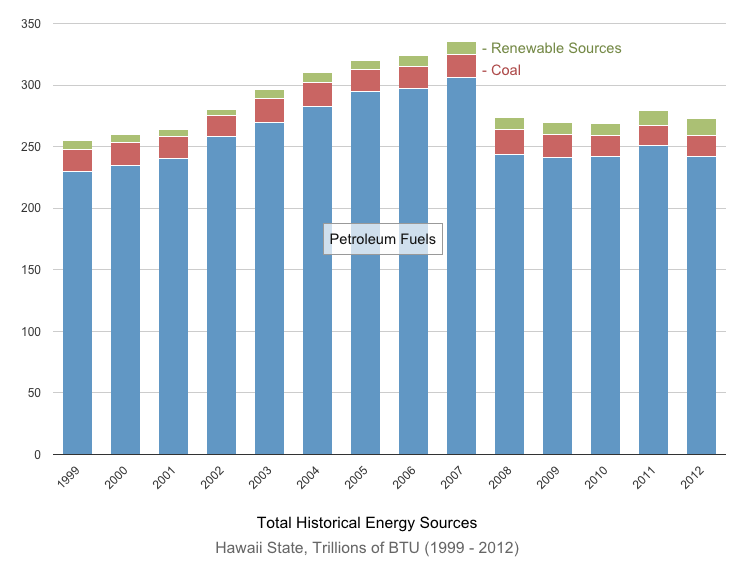
\includegraphics[width=0.6\columnwidth]{hawaii-energy}
		\caption{ Hawaii Energy Sources \cite {hawaiienergypolicy}} 
		\label{fig:hawaii-energy}
\end{figure}

Government action is required to change the balance between methods of generation and consumption. On the other hand, in terms of personal change for a sustainable lifestyle, ``green'' actions addressing responsibility as consumers such as recycling, and saving energy and water need to be pursued \cite{kagawa2007dissonance}.  

changing people's behavior with respect to energy holds significant promise in reducing energy use. Darby's survey of energy consumption research found that identical homes could differ in energy use by a factor of two or more \cite{darby-review-2006}. Data from a military housing community on Oahu show energy usage for similar homes can differ by a factor of 4 \cite{Norton2010ZeroEnergyHomes}.

\section{Collegiate Sustainability Competitions}
\label{sec:rel-competition}

The creation of Makahiki is largely motivated from the needs from colleges and universities in running sustainability competitions for for sustainability education. Energy and water competitions or challenges have been introduced to college dormitories and residential homes as ways to facilitate and incentivize resource reduction to achieve sustainability goals. A survey by Hodge found that there are more than 160 college residence hall energy competitions taking place or being planned for the 2010--2011 academic year in North America~\cite{Hodge2010} to engaging students in sustainability issues. Hodge found that the average reduction in electricity use during these competitions is 9\%. 

A basic type of sustainability competition use a ``minimal tech'' solution such as a web page and manual posting of data and results on a periodic basis such as weekly. The Harvard University Green Cup Competition \cite{harvard-green-cup} and the Wellesley College Green Cup \cite{wellesley-green-cup} are examples of this type of competition. During the 2012 Harvard University Green Cup Competition, there were 4.3\% electricity reduction across the participating residence houses and an individual house reduction of 16.6\%, as shown in \autoref{fig:greencup}.

\begin{figure}[ht!]
	\centering
		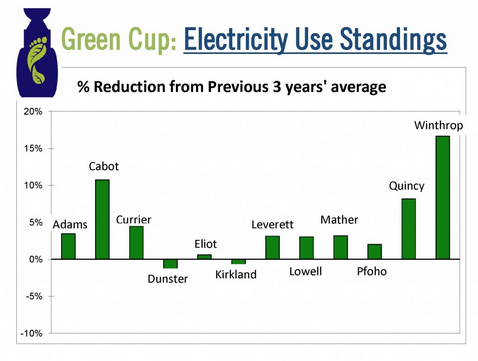
\includegraphics[width=0.6\columnwidth]{harvard-green-cup}
		\caption{Harvard Green Cup Competition for Energy}
		\label{fig:greencup}
\end{figure}

Some organizations built their own custom in-house solutions to support the infrastructure need for sustainability competitions. Oberlin College dorm energy competition \cite{petersen-dorm-energy-reduction}, Duke University's Eco-Olympics competition \cite{duke-eco-olympics}, and Western Washington University 's Go for Green Challenge \cite{Mauney-thesis} are the examples of this type of competition.  Petersen et al. \cite{petersen-dorm-energy-reduction} describe their experiences deploying a real-time feedback system in an Oberlin College dorm energy competition in 2005 that includes 22 dormitories over a 2-week period. The competition used an automated data monitoring system that was developed in house to provide dormitory residents with real-time web-based feedback on energy and water use. They found a 32\% reduction in electricity use across all dormitories and claimed that real-time resource feedback system combined with education and incentives can motivate and empower college students to reduce resource use in dormitories. \autoref{fig:oberlin-design} shows the design of the Oberlin system. 

\begin{figure}[ht!]
	\centering
		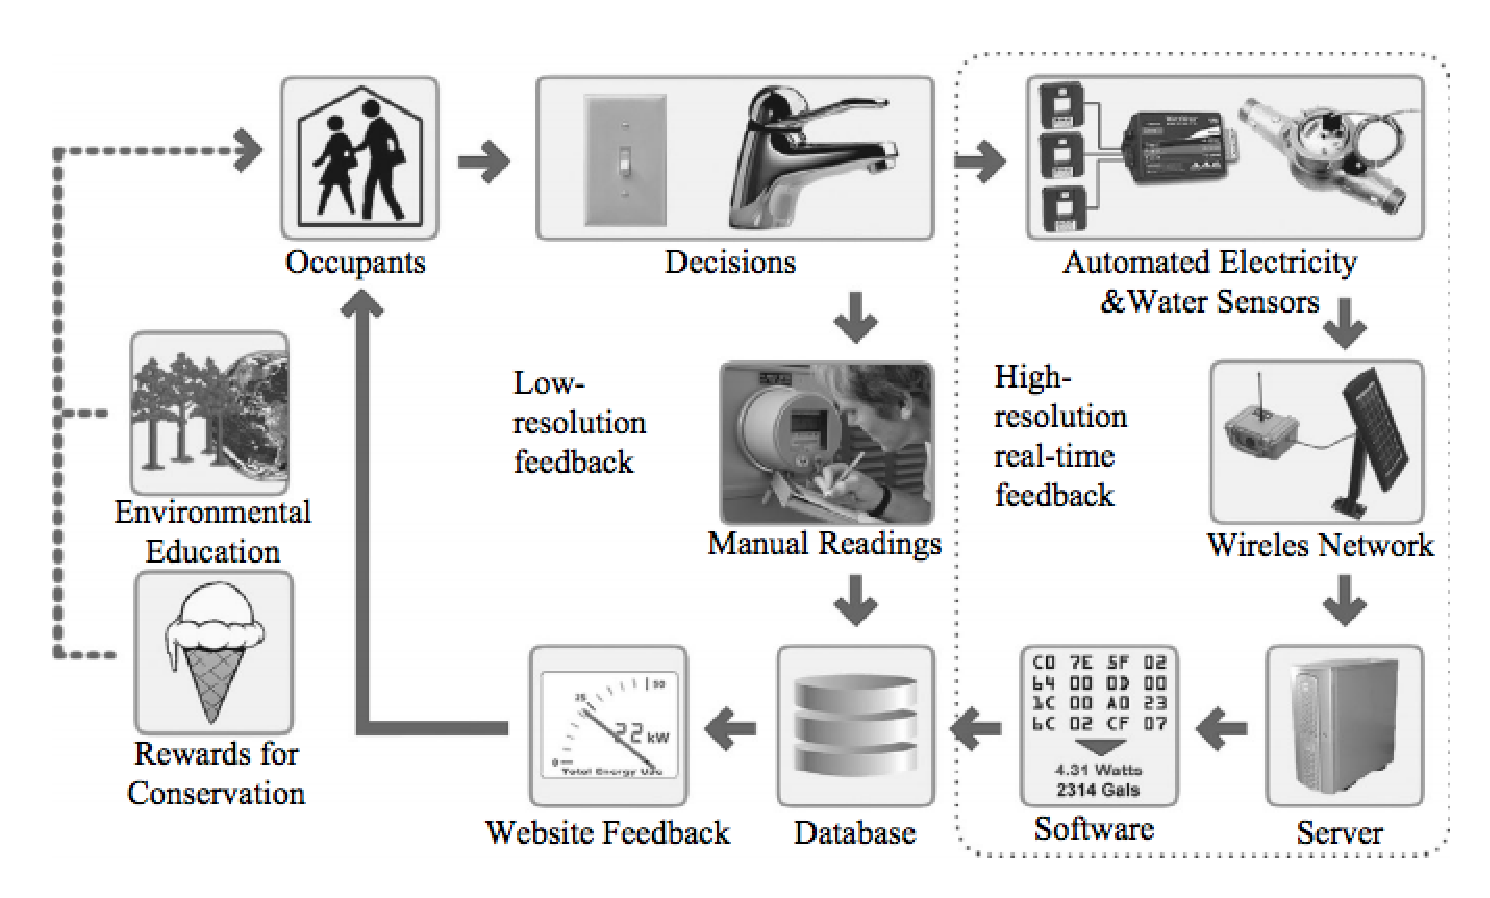
\includegraphics[width=0.6\columnwidth]{oberlin-design}
		\caption{Oberlin College's Custom Designed Sustainability Competition \cite{petersen-dorm-energy-reduction}}
		\label{fig:oberlin-design}
\end{figure}

Universities such as University of British Columbia \cite{runkle2011dark}  and Bowdoin College\cite{bowdoin} chose to out-source the technology to a commercial provider for their sustainability competition. University of British Columbia started the energy competition titled ``Do it in the Dark'' \cite{runkle2011dark} in November 2010 for the 6 first year student residence house. During the competition, the participated residence reduced overall energy consumption by 16.3\%. The competition was hosted by Lucid Design Group's Building Dashboard platform \cite{building-dashboard} which provided the online real-time feedback of energy usage for the participating residence, and other social interaction such as sharing on Facebook through the web interface. \autoref{fig:ubc-do-it-in-the-dark} shows the interface of the University of British Columbia Energy competition using the Lucid's Building Dashboard platform.

\begin{figure}[ht!]
	\centering
		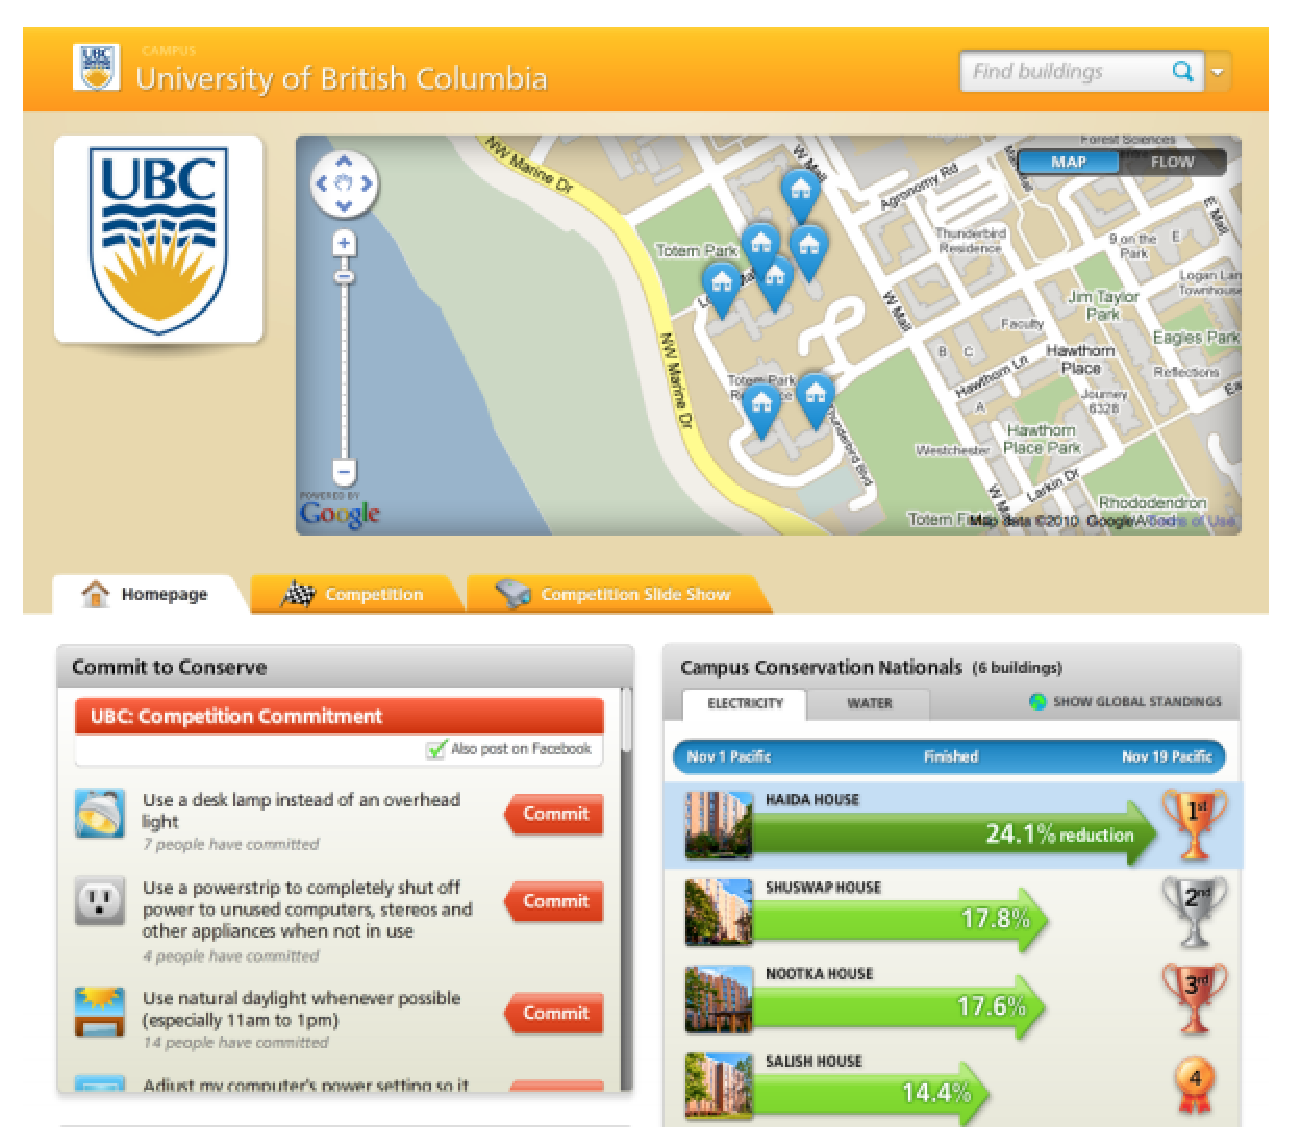
\includegraphics[width=0.6\columnwidth]{ubc-do-it-in-the-dark}
		\caption{University of British Columbia Energy Competition\cite{runkle2011dark} }
		\label{fig:ubc-do-it-in-the-dark}
\end{figure}

Campus Conservation Nationals (CCN) \cite{competetoreduce} is a nationwide electricity and water use reduction competition for colleges and universities. It has been running for the fifth year with hundreds of universities participating across North America. In 2014, 109 schools participated in the Energy Competition, which amount to total 1,330 building in the school campus and total 265,000 students and staffs actively involved in the self-chosen 3 weeks competition. Overall the competition resulted in 4.5\% average electricity competition reduction in the building level, with the top 10 schools achieved reductions ranging from 11\% to 24\%. The software infrastructure used in CCN is supported by Lucid Design Group through its the Building Dashboard platform, which is used by the participating schools to get feedback from their energy and water use, compare performance and track the competition standings.

In summary, these collegiate sustainability competitions have the same goal of engaging students in sustainability issues using resource feedback and incentives such as some kind of prizes. Some competitions also provide educational content or activities such as organizing sustainability related events. Some competitions includes a simple point scheme that participants can win points for their teams or residence dorms by participating in the events and reducing the consumption. The team or dorm with the most points will win the prize. Some competitions also include the social sharing feature such as sharing their commitments to sustainability on Facebook as a way to enforce and encourage the positive behaviors.  \autoref{table:competition} lists the comparison among these competitions. 

\begin{table}[ht!]
  \centering
        \begin{tabular}{| p{5cm} | p{1.5cm} | P{1.8cm} | c | c | p{2.5cm} |} 
        \hline
      \tabhead{School} & \tabhead{Feedback} & \tabhead{Education/ Activities} & \tabhead{Point} & \tabhead{Social} & \tabhead{Infrastructure} \\
                \hline
                Harvard University 	& manual 		& \multicolumn{1}{|c|}{\xmark}	& \xmark 		& \xmark 	& simple webpage\\
                Wellesley College  	& manual 		& \multicolumn{1}{|c|}{\xmark}	& \xmark 		& \xmark 	& simple webpage\\
                Duke University     	& manual 		& \multicolumn{1}{|c|}{\checkmark} & \checkmark & \xmark  & custom website \\
                Duke University     	& manual 		& \multicolumn{1}{|c|}{\checkmark} & \checkmark & \xmark  & custom website \\
Western Washington University & manual 		& \multicolumn{1}{|c|}{\checkmark} & \checkmark & \xmark  & custom website \\
                Oberlin College 	    	& real-time 	& \multicolumn{1}{|c|}{\checkmark} & \xmark 	& \checkmark  & custom website \\
                Bowdoin College 	& real-time 	& \multicolumn{1}{|c|}{\checkmark} & \xmark 	& \checkmark  & out-source \\
   University of British Columbia & real-time      & \multicolumn{1}{|c|}{\checkmark} & \xmark 	& \checkmark  & out-source \\
Campus Conservation Nationals  & real-time   & \multicolumn{1}{|c|}{\checkmark} & \xmark 	& \checkmark  & out-source \\
                \hline
        \end{tabular}
        \caption{University energy competitions}
        \label{table:competition}
\end{table}

None of these choices are ideal: the custom in-house solution requires sophisticated design and implementation skills; out-sourcing can be financially expensive and impedes evolution; and the simple webpage solution does not fully leverage the possibilities of advanced information technology.

The goal of Makahiki is to provide an open source framework for different organizations to create engaging sustainability serious games, including this kind of sustainability competitions. In addition to provide improvements to all of features discussed above, Makahiki creates a more game-like interface such as tracking individual points and game plays, level progression and raffle game etc. Makahiki lowers the overhead to those who would build a custom in-house solution by providing pre-built components. It can lower the financial cost to those who would out-source by providing an open source alternative. Finally, it provides an opportunity for those who would choose a minimal tech solution to instead provide more sophisticated information technology.

\section {Serious Games and Gamification}
\label{sec:rel-seriousgame}

Differentiating Makahiki from the other collegiate sustainability competition is the game design elements in Makahiki. We consider the sustainability competitions that created by the Makahiki framework are of a type of serious games.  A serious game is ``a game designed for a primary purpose other than pure entertainment'' \cite {WikipediaSeriousGame}. It includes categories such as educational games and advergames (advertising), political games, and training games (also known as game-learning). Zyda \cite{Zyda2005} defines serious game as ``a mental contest, played with a computer in accordance with specific rules that uses entertainment to further government or corporate training, education, health, etc''. 

One prominent example is Foldit \cite {khatib2011crystal}, a multiplayer online game which helps solving problems that computers can not solve very well. In this case, online gamers around the world together were able to do what biochemists have been trying to do for a decade: decipher the structure of a protein that is key to the way HIV multiplies. \autoref{fig:foldit} shows a screen shot of the Foldit game.

\begin{figure}[ht!]
	\centering
		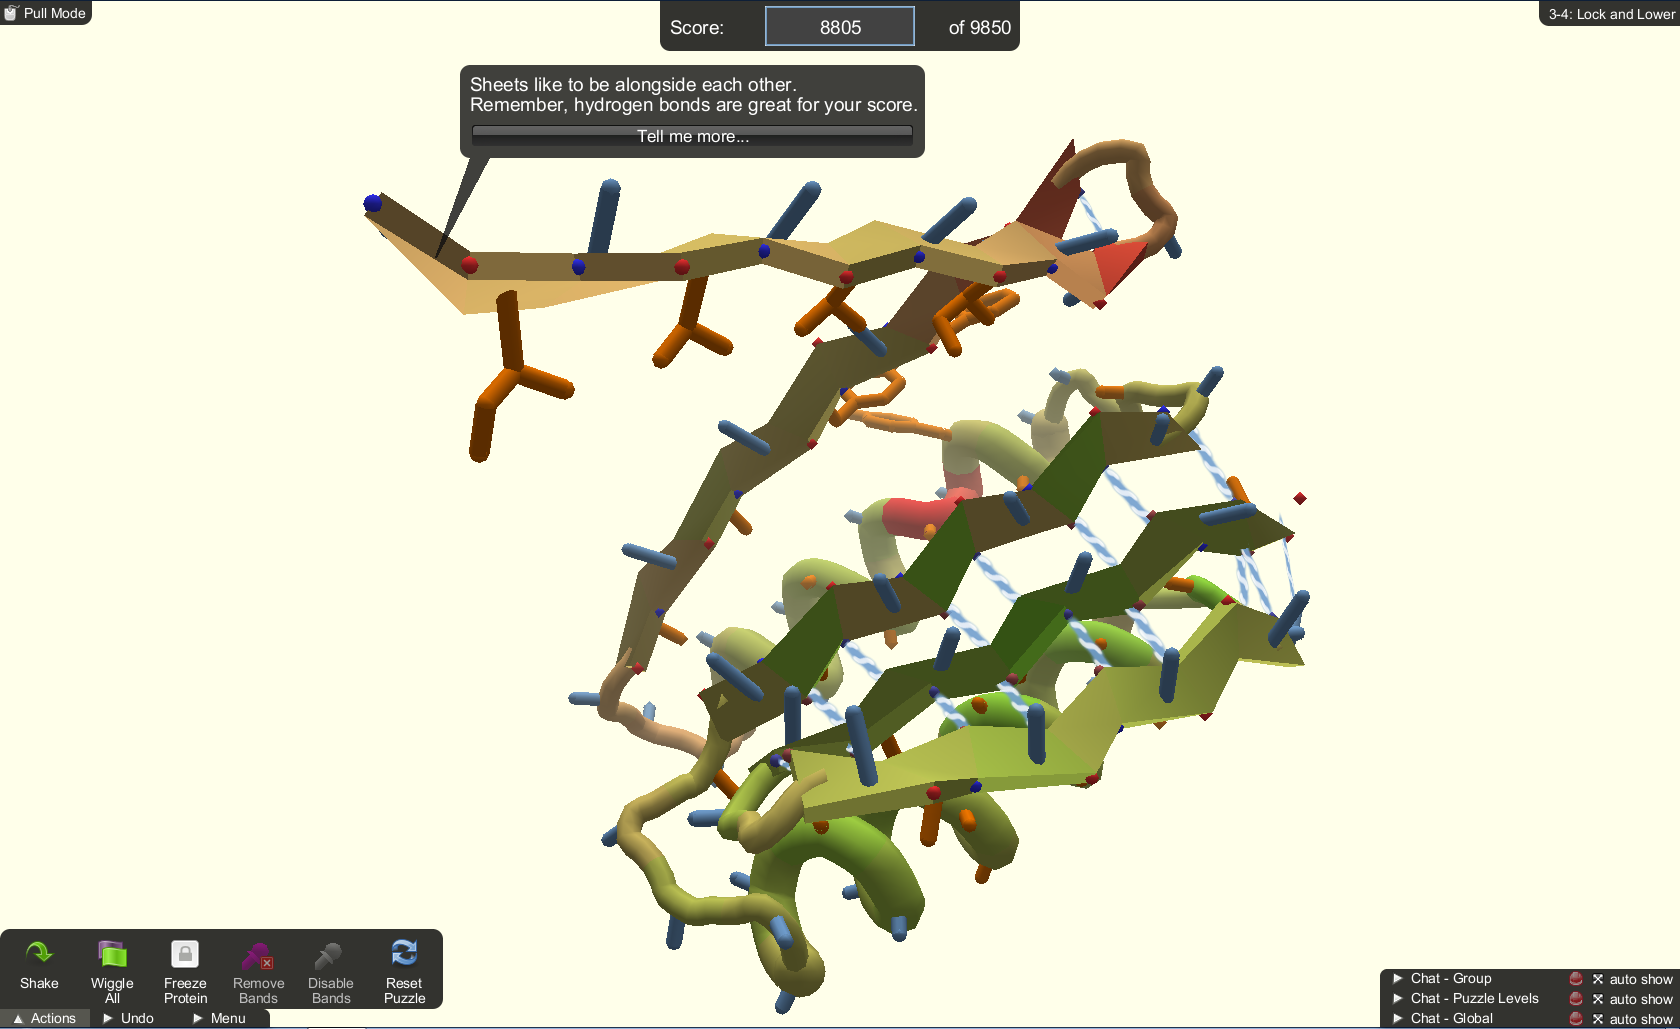
\includegraphics[width=0.6\columnwidth]{foldit.eps}
		\caption{Serious Game Example: Foldit is solving a serious problem \cite {khatib2011crystal}} 
		\label{fig:foldit}
\end{figure}

An Alternative Reality Game (ARG) is one type of serious game that blends real and virtual world activities in the serious gaming context. McGonigal defines ARG as ``games you play to get more out of your real life, as opposed to games you play to escape it'' \cite{mcgonigal2011reality}. Her award winning serious ARG game ``World Without Oil'' \cite{worldwithoutoil} and ``Evoke'' \cite{urgentevoke} are designed with the goal of empowering people to come up with creative solutions to urgent real-world problems. \autoref{fig:worldwithoutoil} shows an screen shot of the World Without Oil game. The game started on April 2007 for 32 days and concluded on June 2007. Approximately 2000 players participated in the game. They were asked to imagine what life would be like without oil, or try actually living without oil, then post their stories and thoughts in the forms of letter, emails, voicemails, blog posts, online videos and images. Some players reported that the online game affected their real world behaviors in some ways\cite{mcgonigal2011reality}.

\begin{figure}[ht!]
	\centering
		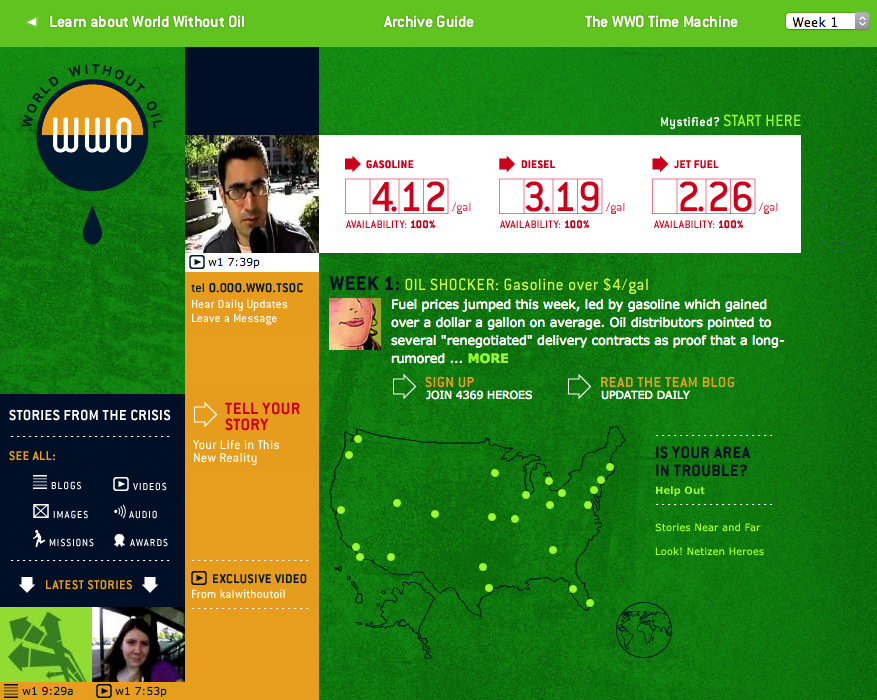
\includegraphics[width=0.6\columnwidth, height=3.5in]{worldwithoutoil}
		\caption{Serious Game Example: World Without Oil - Play it before you live it. \cite{worldwithoutoil}}
		\label{fig:worldwithoutoil}
\end{figure}

ARGs have also been used to support learning. Connolly et al. \cite{connolly2009arguing} discuss the development of an educational ARG to motivate secondary school students across Europe to learn foreign languages. The results of the pilot run of the game in 2009 indicated that 92\% of students felt the game motivated them to learn a second language. One of problems the team identified is the limitation of Moodle \cite{moodle} platform the game is based on and there is potential to improve the effectiveness of the game.

The report of the ARGOSI project \cite{whitton2009alternate} provides insights into the use of ARGs in game based learning and the challenges they face in the field of higher education. The pilot was run at the University of Bolton with the aim of providing an engaging alternative to traditional methods of introducing students to university life. Adoption of the game was fairly low with 173 players and 23 (13\%) of whom were active. The project identifies a number of questions surrounding educational ARGs, such as motivation, relationship to curriculum, marketing and timing. The report suggests that a complete ARG model may not be appropriate for wholesale learning, but there is certainly potential in using game elements.

Makahiki shares similarity with the ARGs that they both combined real and virtual world activities to achieve ``serious'' purposes, be it educational or behavior changing. 

While ``Serious Games'' has been an active research topic for decades, ``Gamification'', on the other hand, is a relatively new subject. Deterding et al. \cite {Deterding2011mt} defines gamification as ``the use of game design elements in non-game contexts''. The term only came into widespread use starting in 2010 \cite {schell2010design} \cite {zichermann2010game}. Gartner \cite {gartnerPress2011} predicts that by 2015, more than half of companies managing innovation processes will employ gamification, applying game mechanics to application areas including productivity, finance, health, sustainability, news, user-generated content and e-learning. 

Deterding et al. \cite{Deterding2011mt} describes the distinctions between gamification, serious games and other related concepts, as shown in \autoref{fig:define_gamification}. According to Deterding, a) Gamification is about games. It is different than playful interaction or playful design. b) Gamification uses game elements. It is not a complete game such as a serious game. c) Gamification applies to non-game contexts. Similar to serious games, gamification uses games for other purposes than its normal expected use for entertainment. d) Gamification focuses on design. It is not game-based technology or practice of wider game ecology.

\begin{figure}[ht!]
	\centering
		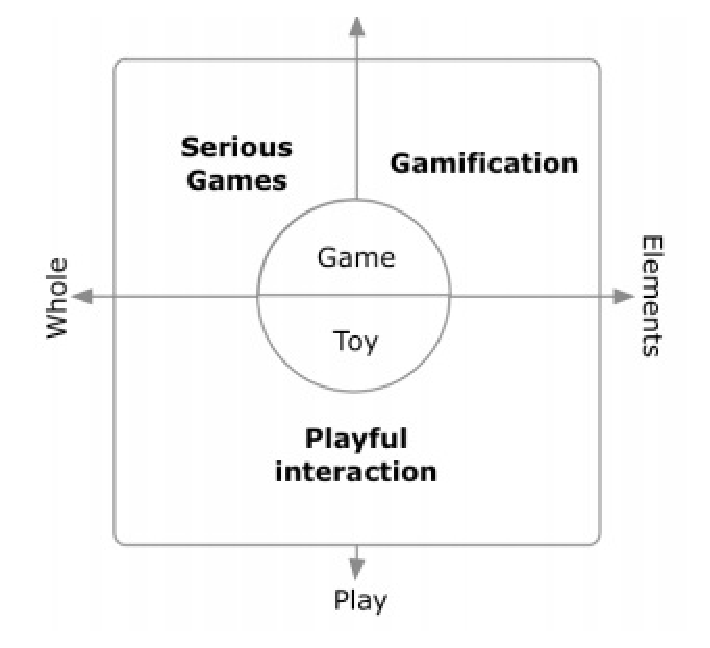
\includegraphics[width=0.5\columnwidth]{defining_gamification.eps}
		\caption{Serious Game and Gamification (source: Deterding \cite{Deterding2011mt})}
		\label{fig:define_gamification}
\end{figure}

The system created by Makahiki consists of a number of smaller games which combined,  provides a game playing experience to the participants. So we consider that Makahiki framework produces a serious game, instead of a gamified educational application. While they are different, both gamification and serious games are trying to solve problems with game thinking. Gamification's main driving force is motivation, similarly, serious games also try to solve the motivation problem and influence people's behavior for ``serious'' purpose.  Bosch \cite{bosch2011} considered the serious game Foldit as a successful example of gamification in science. 

FourSquare \cite{foursquare} is probably the most recognized example of applying game mechanics to a location based networking application. It is a location based game like service where players check-in to locations for virtual points and rewards.  By employing gamification elements such as points, badges, levels and leader boards, it engages users to revisit a location such as a restaurant or pub and become a loyal customer and finally the ``mayor'' of the place. Certain virtual rewards such as the ``mayor'' of a particular Starbucks can be converted into real products, e.g. a free coffee. Foursqure proved that simple game mechanics can affect user behavior by engaging 10 million customers with a successful business model. \autoref{fig:foursquare} shows the home page for FourSquare.

\begin{figure}[ht!]
	\centering
		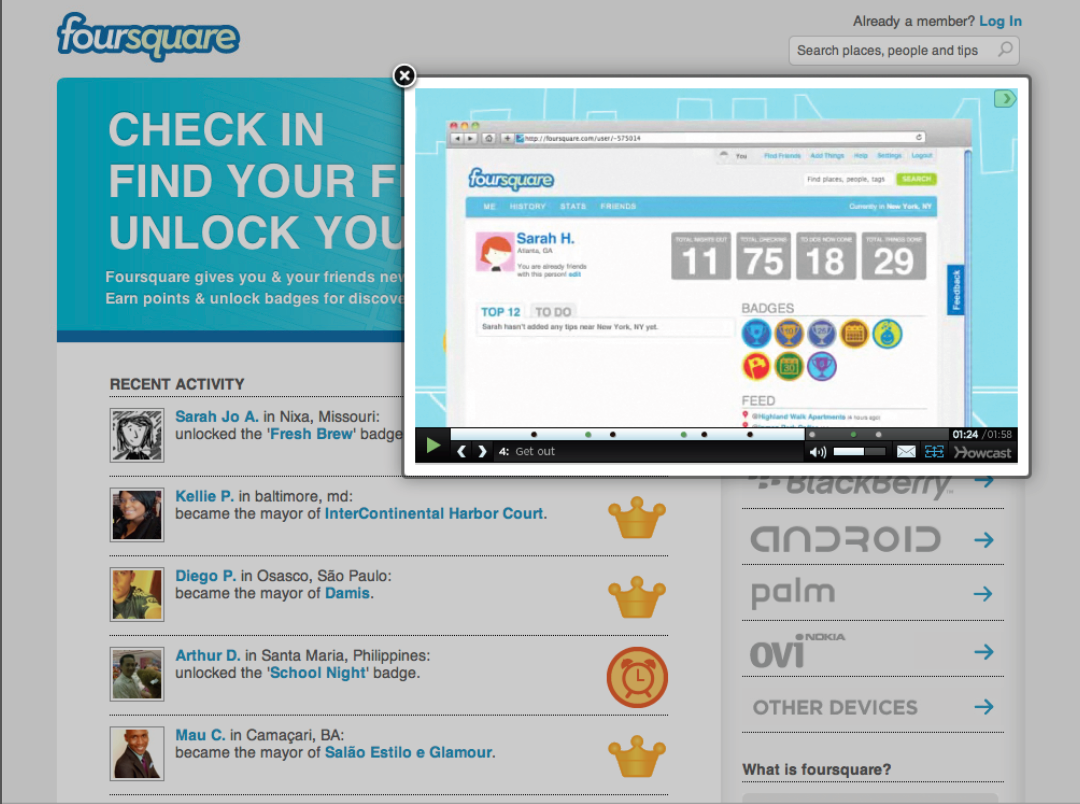
\includegraphics[width=0.7\columnwidth]{foursquare.eps}
		\caption{Gamification Example: Foursquare makes modern badges popular\cite{foursquare}}
		\label{fig:foursquare}
\end{figure}

Nike+ \cite{nikeplus} is a social running game that employs game mechanics to encourage runners - both casual and hardcore - to compete and improve their fitness, with the goal of solving the main problem of most fitness programs: motivation. Nike+ allows runners to upload their exercise data to its web site, and start challenging themselves and their friends. They can also get support from their friends through the web site. The game makes running and exercise fun, which eventually serve the ``serious'' purpose of making people healthy. \autoref{fig:foursquare} shows the home page for Nike+.

\begin{figure}[ht!]
	\centering
		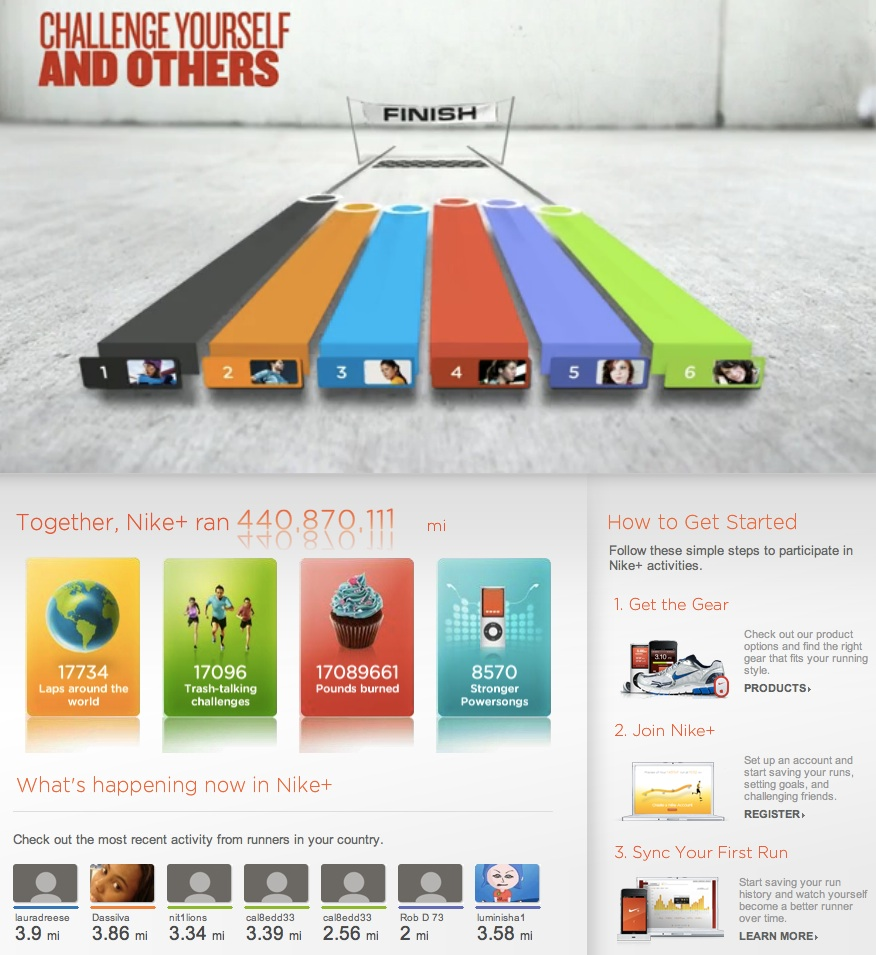
\includegraphics[width=0.7\columnwidth,height=3in]{nikeplus.eps}
		\caption{Gamification Example: Nike+ makes fitness run\cite{nikeplus}}
		\label{fig:nikeplus}
\end{figure}

RibbonHero \cite{ribbonhero} is a game that helps users discover new Microsoft Office features, as shown in \autoref{fig:ribbon}. The goal is to have users build familiarity and expose them to the Office UI, so that they understand what kind of features are available. According to the creator of the game, Office ``has a lot of powerful features that users might not know but can be really useful''. The game gives users a chance to learn those features through a game interface, rather than reading the software manuals or watching the typically dry IT training videos.

\begin{figure}[ht!]
	\centering
		\subfigure[Quest to earn points]{\label{fig:Ribbon1}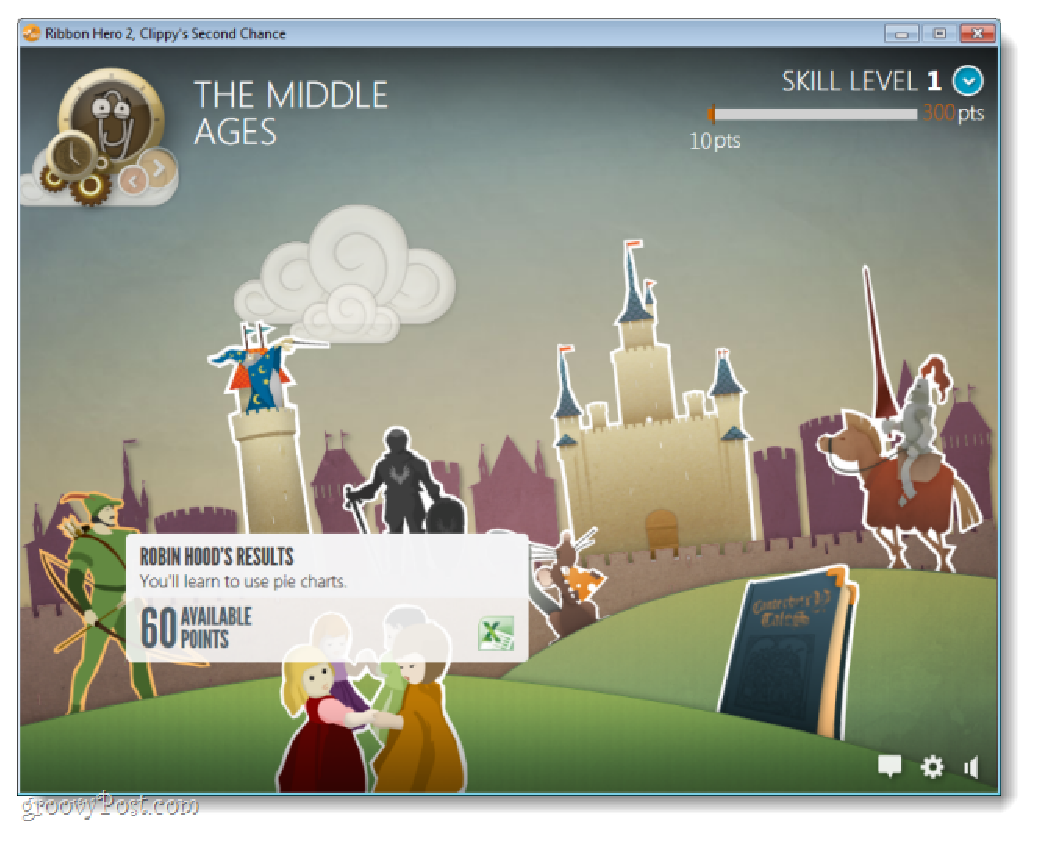
\includegraphics[height=2.5in]{ribbon1.eps}}
		\subfigure[Competing a task]{\label{fig:Ribbon2}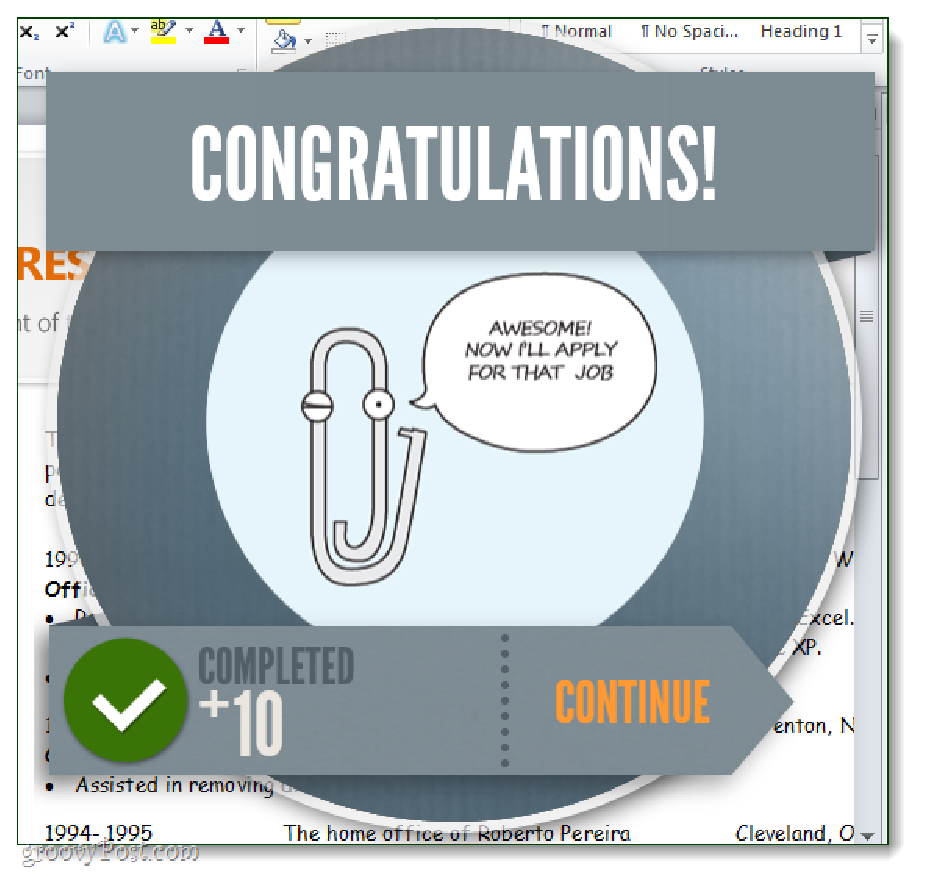
\includegraphics[height=2.5in]{ribbon2.eps}}
		\caption{Gamification Example: RibbonHero Helps to Learn Office\cite{ribbonhero}}
		\label{fig:ribbon}
\end{figure}

Interactive design also applies game elements in their design to achieve sustainability goal. One example is the ``SmartGauge'' dashboard (\autoref{fig:ixd-dashbard}) \cite {ideo2009} for Ford's hybrid cars, where a digital plant responds to how energy-efficient the users driving behavior is. The design gives drivers a game, with the goal to grow more lush and beautiful leaves, a visual reward, by driving efficiently and thus promotes a more environmental behavior. Similarly, The design of ``Piano Staircase'' (\autoref{fig:ixd-pianostair}) \cite {funtheory2009}, created by Volkswagen Sweden, installed in a metro station in Stockholm, is to make the staircase next to the escalator look and respond like a piano keyboard, so that every step on the stair will generate different piano sounds every time a commuter walked on it. Observation indicates that 66 percent more people chose to play the ``piano staircase'' game over using the escalator. It is a good example of gameful design for persuading and encouraging energy-efficient behavior. 

 \begin{figure}[ht!]
	\centering
		\subfigure[Efficiency Leaves]{\label{fig:ixd-dashbard}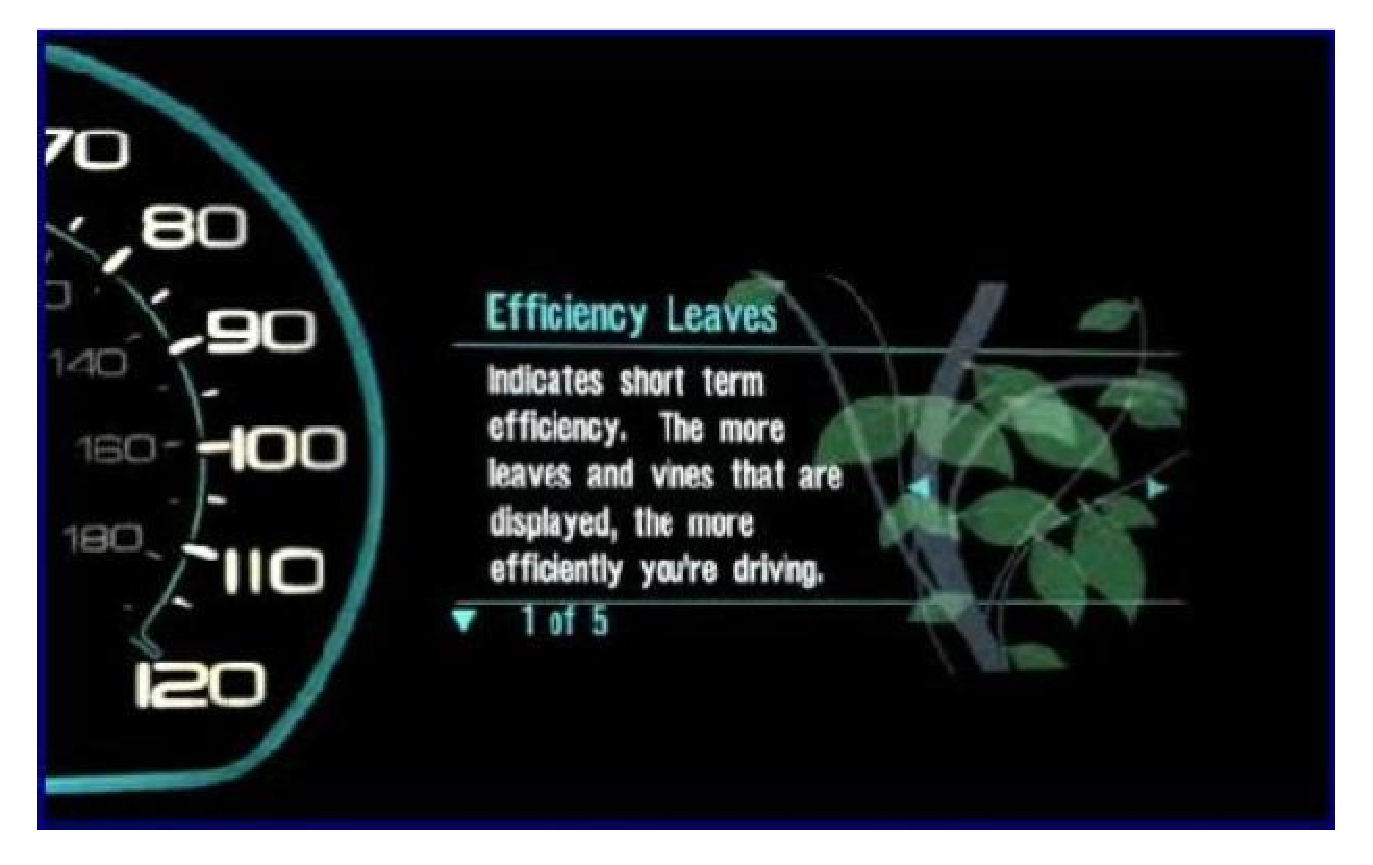
\includegraphics[width=0.6\columnwidth]{ixd-dashboard.eps}}
		\subfigure[Piano Stair vs. Escalator]{\label{fig:ixd-pianostair}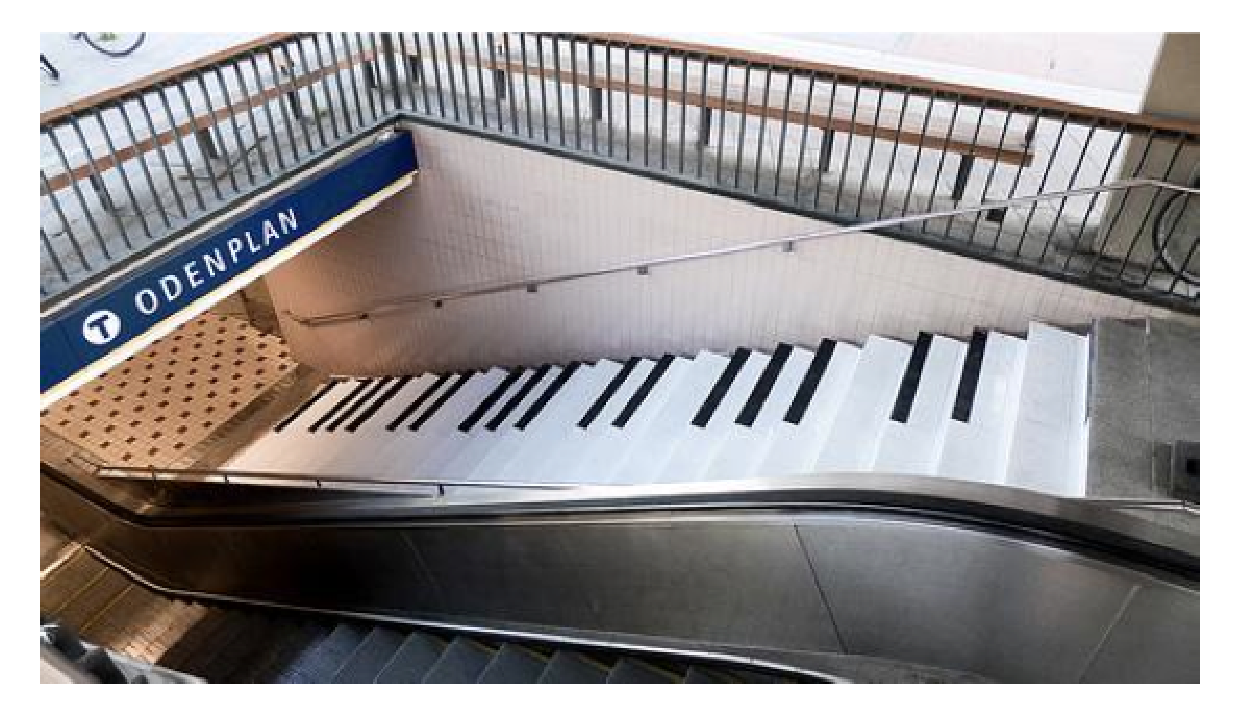
\includegraphics[width=0.6\columnwidth]{ixd-pianostair.eps}}
		\caption{Gameful Design for Sustainability}
		\label{fig:ixd}
\end{figure}	

Persuasive game is another genre of video game that use game design to influence player behaviors. In his book ``Persuasive Games, The Expressive Power of Video games'', Ian Bogost\cite{bogost2007persuasive} argues that persuasive games have a unique persuasive power that goes beyond other forms of computational persuasion. Not only can
persuasive games support existing social and cultural positions, as in serious games, but they can also
disrupt and change those positions, leading to potentially significant long-term social change. Persuasive game is closely tied to ``Persuasive Technology''\cite{fogg_2003}, designed to change attitudes or behaviors of the users through persuasion and social influence, but not through coercion. Loren Baxter\cite{baxter_2011} posted that persuasive design, the use of psychology in design to influence behavior, could benefit UX design in a new level.

\section{Game Design and Motivation}
\label{sec:game-design}

The research in serious games and gamification inspires the design of Makahiki in terms of benefits of a game, game design and how the game design can motivate and engage players in serious contexts. 

Why games? Results of a study published in the May 1998 issue of Nature \cite {koepp1998evidence} demonstrated that video game players experience regular releases of dopamine during game play. Dopamine is a neurotransmitter that signals pleasure rewards for food, sex and addictive drugs, such as cocaine. 

A favorite subject of Greek vase paintings in the ancient games exhibition in the British Museum's department of Greek and Roman antiquities is Ajax and Achilles playing a kind of board game called backgammon, as illustrated in \autoref{fig:ancient-games}. It is noteworthy that both Ajax and Achilles have the full armor on while playing the game. According to Arthur A. Krentz \cite{krentz1998play}, in Plato's ``Republic'', the term ``paideia" (in Greek, means education/culture), ``paidia" (means play/game/pastime/sport), and ``paides" (means children), have the same root. The three terms often show up in the same context. Krentz states that ``The central aim of pedagogy (paidagogia) is to encourage learning as a form of play (paidia), which is the most persuasive and effective approach to learning" .

\begin{figure}[ht!]
	\centering
		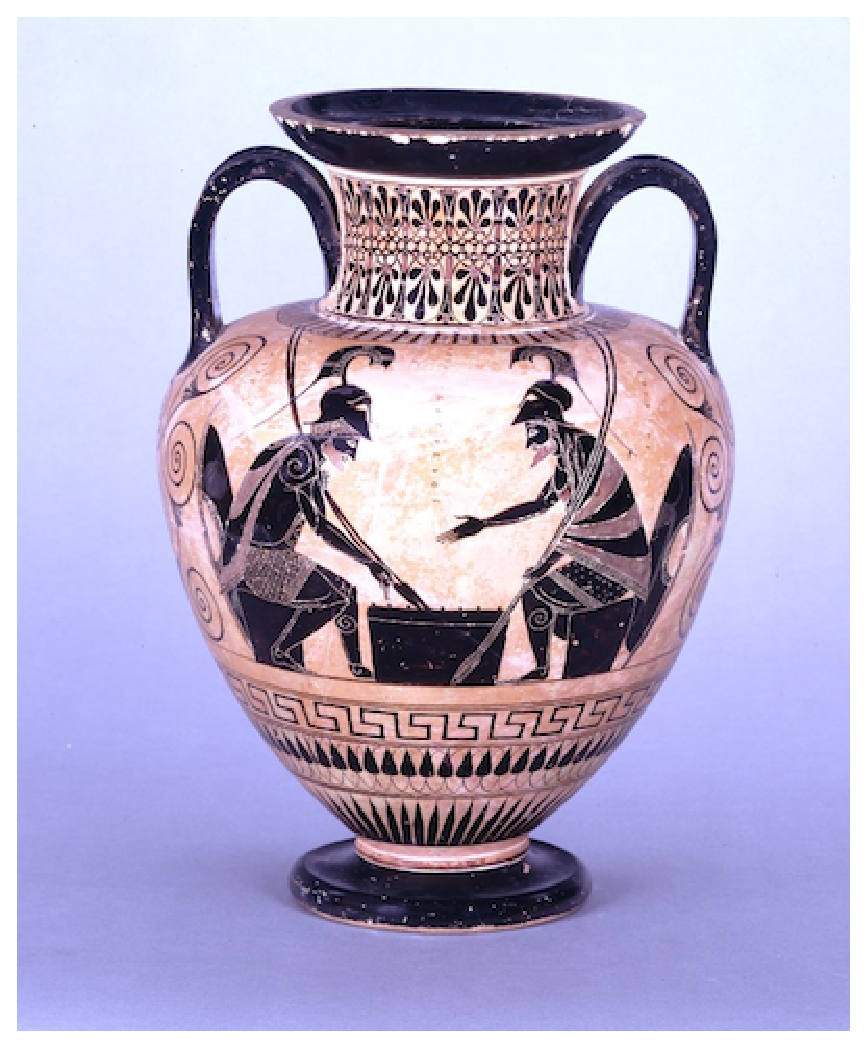
\includegraphics[width=0.4\columnwidth]{roman-game-vase.eps}
		\caption{Ancient Games Shown in British Museum}
		\label{fig:ancient-games}
\end{figure}

Moving forward a couple of millennia, World of Warcraft (WoW) is a massively multiplayer online role-playing game (MMORPG) with 11.1 million subscribers, currently the world's most popular MMORPG.  Nick Yee \cite {yee2002understanding} pointed out that the collaborative nature of most activities makes MMORPG unique. ``It's the people that are addictive, not the game''. ``Most importantly, it is the reward of being socialized into a community of gamers and acquiring a reputation within it''  . He claimed \cite {yee2001vsb} that ``WoW truly is a virtual Skinner box'', smoothly increasing reward and difficulty and reinforcing player commitment along the way.
	
In her popular and inspiring TED talk ``Gaming can make a better world" \cite {mcgonigal2010ted} and in her book ``Reality is Broken" \cite {mcgonigal2011reality}, researcher and game designer Jane McGonigal makes a case for why good games make us better, and how they can help us change the world. She notes that more than 3 billion hours a week is spent in playing video game by our society. She says that the average gamer plays 10,000 hours of games by age 21. That's about the same number of hours that students spend in high school and middle school. There are 500 million gamers today, playing on all sorts of platforms from the iPhone to game consoles. Instead of the common conception that gaming is a waste of time, she argues that ``playing games is the single most productive thing we can do with our time'' and that is  the solution to our ``Broken Reality''. Byron Reeves also argues in his book ``Total Engagement" \cite {reeves2009total}, that games, especially MMO type games, can change the way people work and businesses compete.

Psychology professor Mihaly Czikszentmihalyi introduced a specific kind of happiness that he named ``flow" \cite{csikszentmihalyi1991flow}, which is considered as one of the fundamental reasons that people play games \cite{murphygames}. Flow is a state of absorption, characterized by intense concentration, loss of self-awareness, a feeling of being perfectly challenged (neither bored nor overwhelmed) and a sense that time is flying. In order to achieve flow, the important condition is a balanced goal that is challenging yet achievable within the individual's ability. This balance is referred to as the flow channel as shown in \autoref{fig:state_of_flow}.

\begin{figure}[ht!]
	\centering
		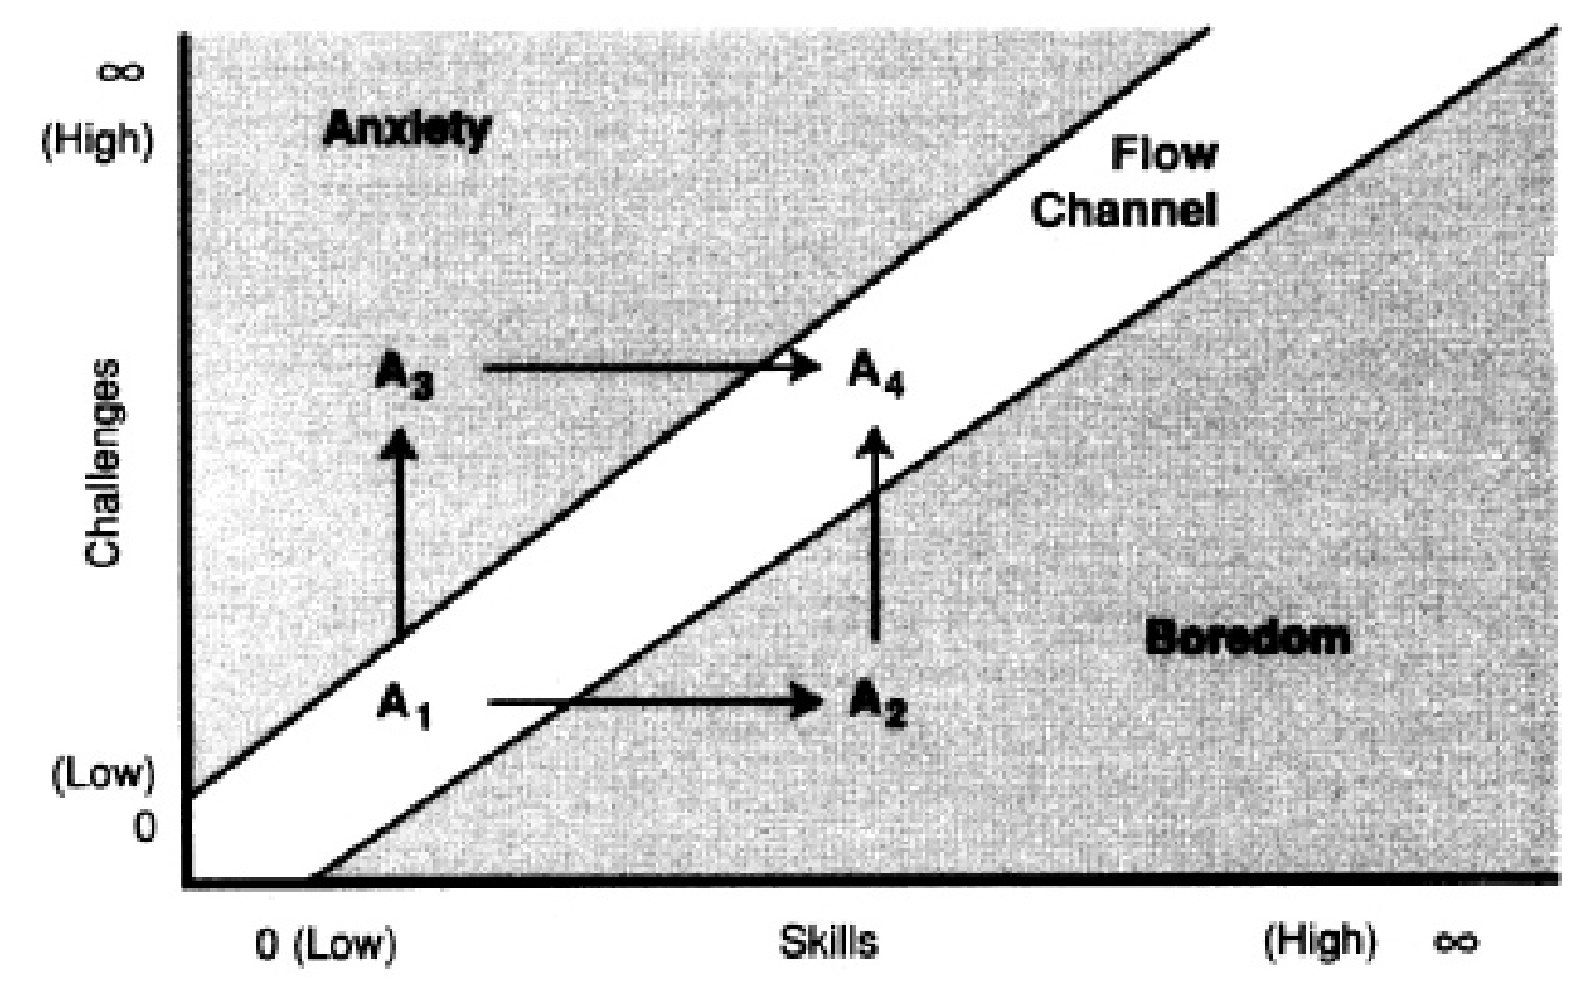
\includegraphics[width=0.7\columnwidth]{flow.eps}
		\caption{The state of flow is achieved between anxiety and boredom (source: Czikszentmihalyi \cite{csikszentmihalyi1991flow})}
		\label{fig:state_of_flow}
\end{figure}

In order to understand why people play games, Richard Bartle identified four player personality types by studying players of the Multi-User Dungeon (MUD) game in 1960s \cite {bartle1996hearts}:
\begin{enumerate}

\item \textbf{Achievers}: driven by in-game goals, usually some form of points gathering - whether experience points, levels, or money.

\item \textbf{Explorers}:  driven to find out as much as they can about the virtual construct - including mapping its geography and understanding the game mechanics.

\item \textbf{Socializers}: use the virtual construct to converse and role-play with their fellow gamers.

\item \textbf{Killers}: use the virtual construct to cause distress on other players, and gain satisfaction from inflicting anxiety and pain on others.

\end{enumerate}

Bartle's player type model has been the basic for understanding the player motivation. Dan Dixon presented the limitation and misuse of Bartle's model in general games and gamification contexts \cite{DixonPlayerType}. Amy Jo Kim applied the model in her gamification approach by overlaying social actions from the game on top of the player types \cite {Kim2010}, as shown in \autoref{fig:play-types}.

\begin{figure}[ht!]
	\centering
		\subfigure[Bartle's Player Types (1996)]{\label{fig:player-types}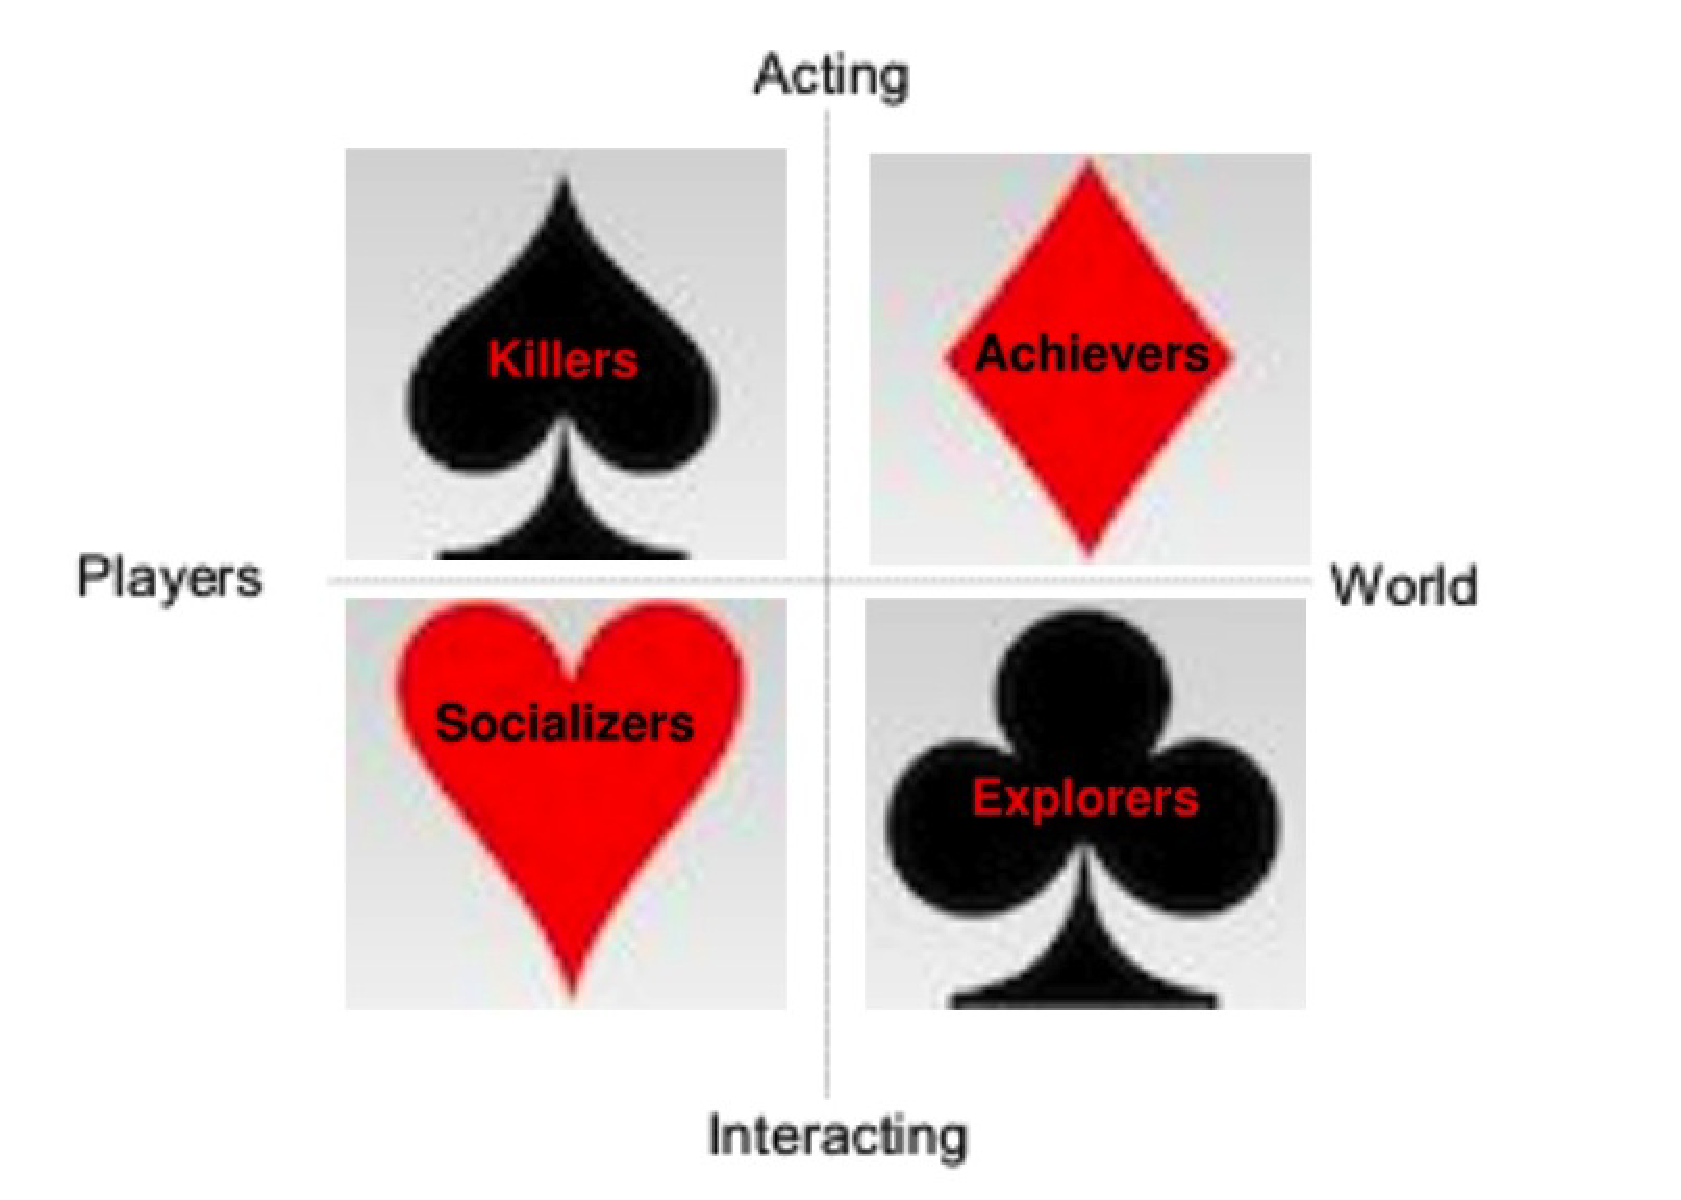
\includegraphics[height=2.1in]{bartle-player-types.eps}}
		\subfigure[Kim's Social Actions (2010)]{\label{fig:social-action}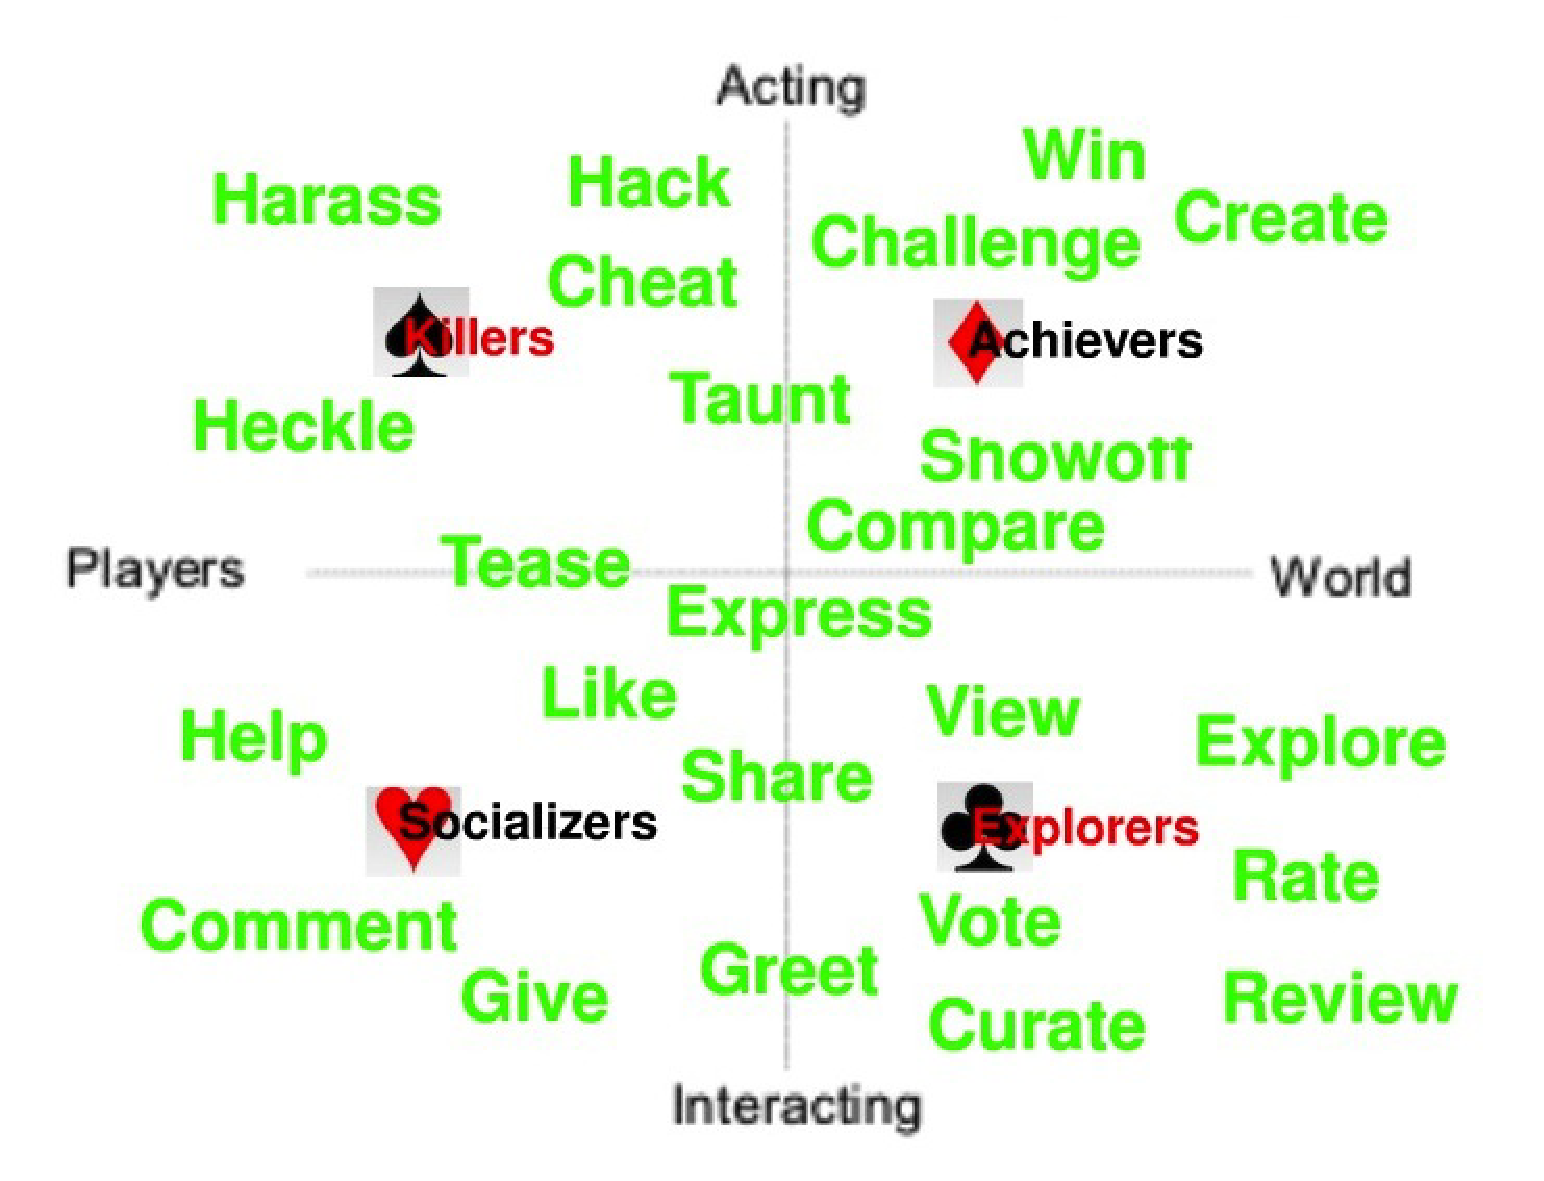
\includegraphics[height=2.1in]{kim-player-types.eps}}
		\caption{Player Types}
		\label{fig:play-types}
\end{figure}

Different game mechanics and elements can be used to serve different functions in satisfying players' needs, and the basic elements such as points, badges, and leader boards are the defining attributes of the current gamification practices \cite {Deterding2011dragon}. \autoref{fig:basic-game-elements}  illustrates these basic game mechanics and elements.

\begin{figure}[ht!]
	\centering
		\subfigure[Satisfies Human Needs (source: Bunchball\cite{bunchball})]{\label{fig:human-needs}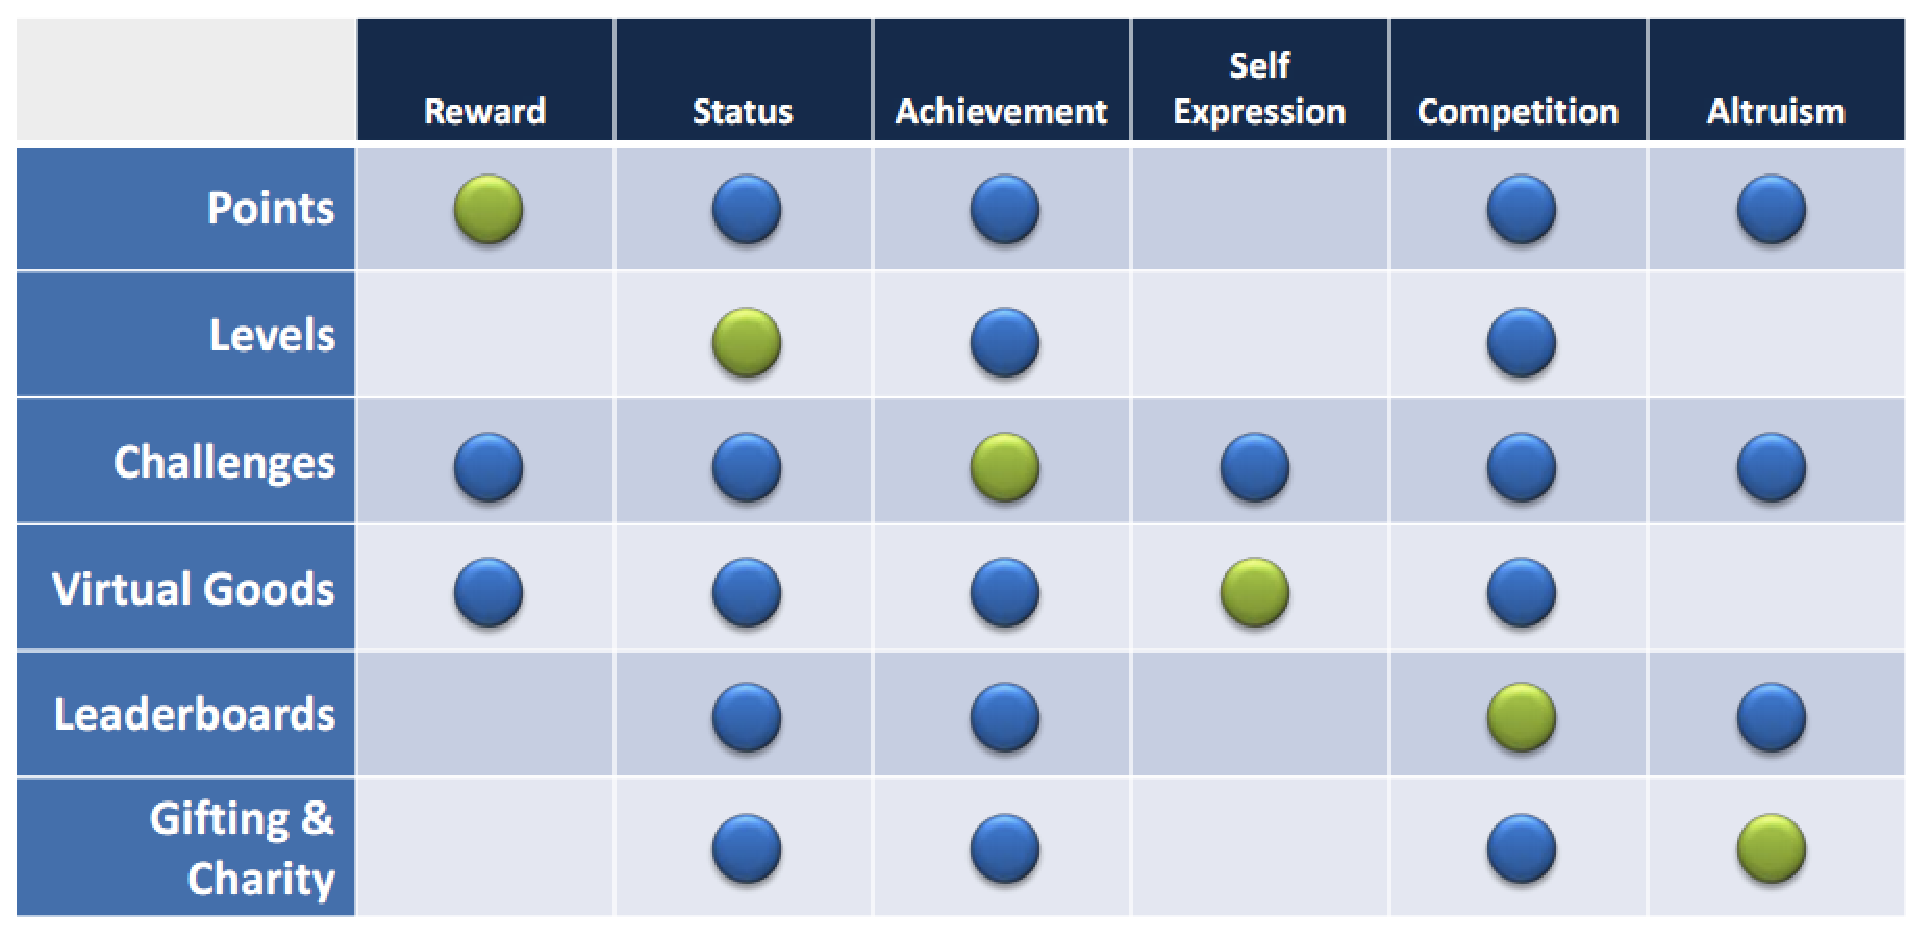
\includegraphics[width=3.8in]{human-needs.eps}}
		\subfigure[Basic Mechanics (source: Deterding \cite{Deterding2011meaningful})]{\label{fig:basic-elements (source: }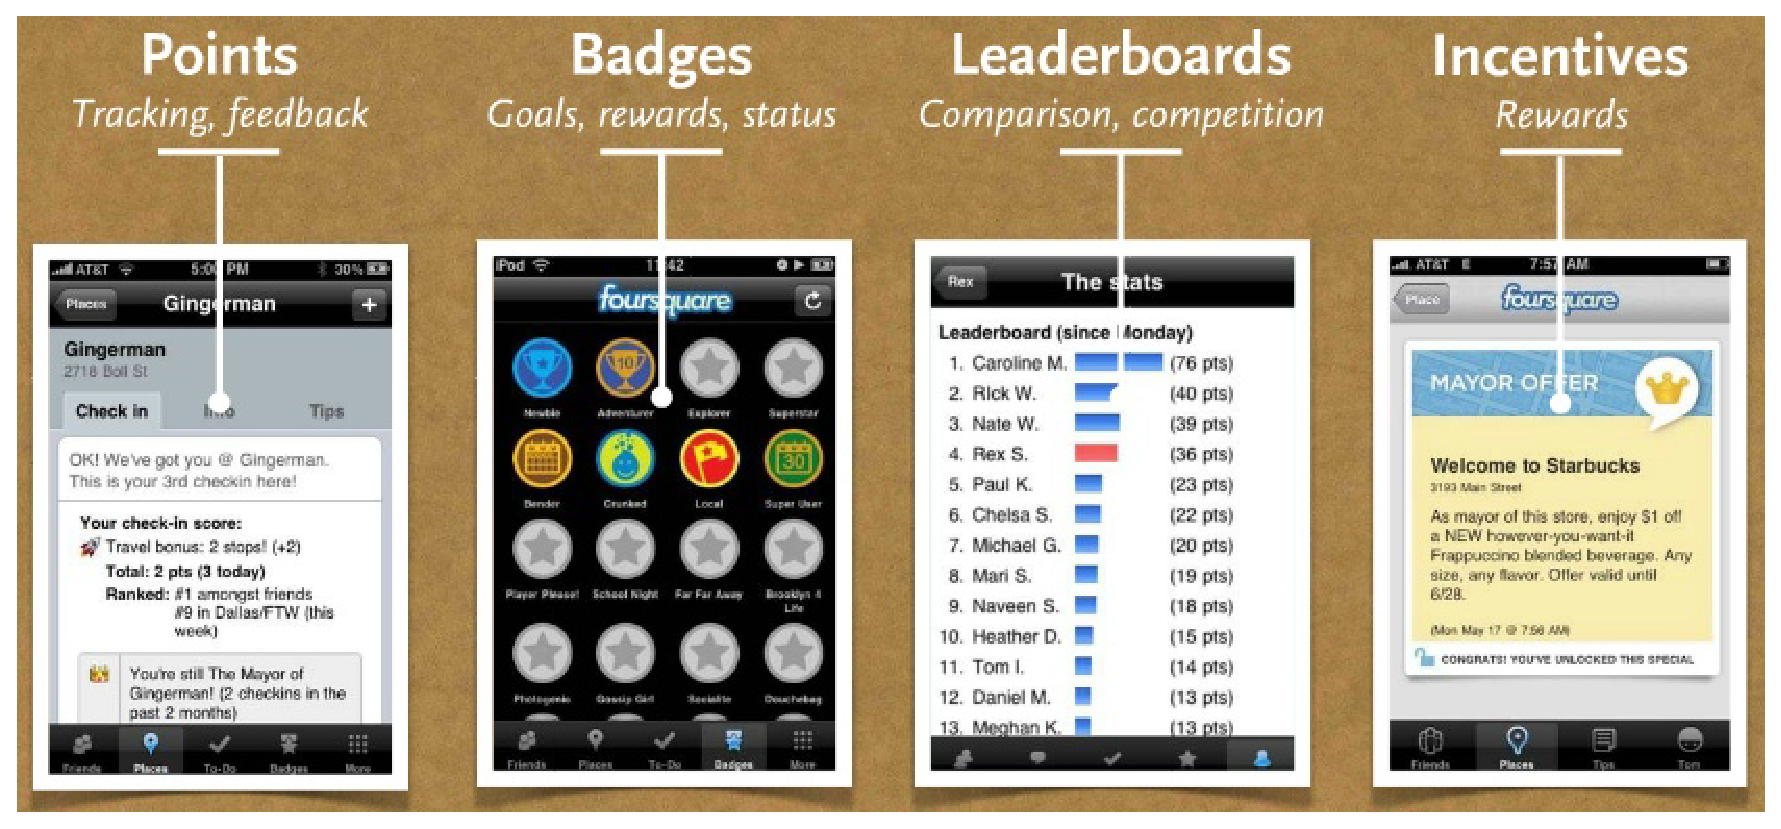
\includegraphics[width=3.8in,height=2in]{basic-element.eps}}
		\caption{Basic game mechanics and elements}
		\label{fig:basic-game-elements}
\end{figure}

Seth Priebatsch \cite {Priebatsch2010ted} stated that you can get anyone to do anything with 7 game dynamics. Techcrunch \cite{Biggs2010} published a ``secret'' game dynamics play deck that is used by Priebatsch's company SCVNGR. The play deck is a set of 47 flash cards. Each card illustrates one game dynamics. SCVNGR employees are instructed to memorize them and apply in their applications as needed.  

There are many debates and criticism over whether gamification itself is inherently good or bad. 
Many considered the current efforts of gamification focus on extrinsic motivators (such as points, badges and rewards) instead of intrinsic motivators generated by an individual's internal will or desires.

Designer Stephen Anderson claimed that gamification mistakes extrinsic rewards (rather than intrinsic motivation) for the power of games and hence offers only feedback, not goals \& rules \cite {anderson2011}. 

\begin{figure}[ht!]
	\centering
		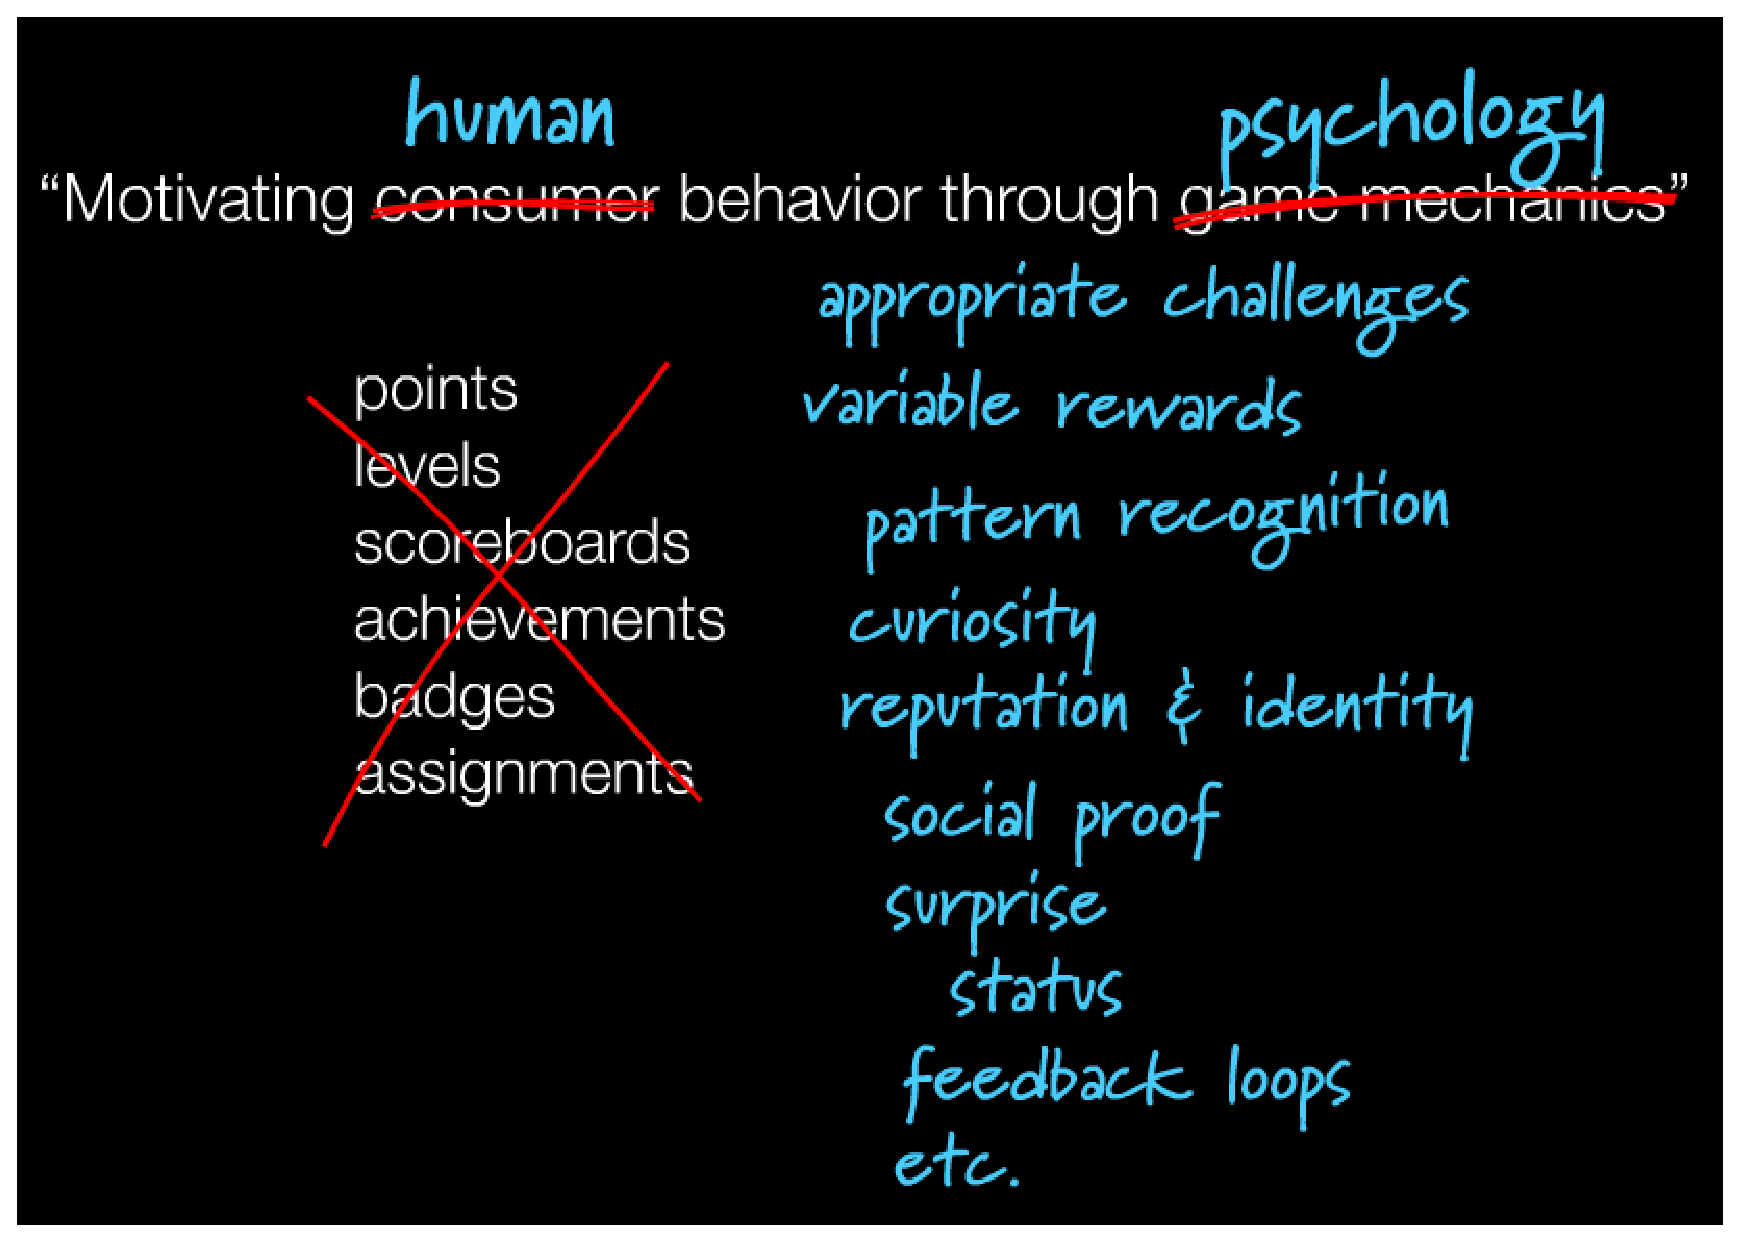
\includegraphics[width=0.6\columnwidth]{anti-gamification.eps}
		\caption{Gamification is about extrinsic rewards (source: Anderson \cite {anderson2011})}
		\label{fig:anti-gamification}
\end{figure}

Jane McGonigal spoke about her concern about current state of gamification in the GDC 2011 talk titled ``We don't need no stinking badges: How to reinvent reality without gamification'' \cite {mcgonigal2011}. She argued that current gamification confuses intrinsic/extrinsic motivation and proposed ``Gameful Design'' instead of ``Gamification''. She claimed that "Gameful is player-oriented", which presumed that the loyalty program type gamification is product or service oriented. While the current gamification is about extrinsic reward, with points, badges, and levels, gameful design is about intrinsic reward, with positive emotion, relationships, meaning and accomplishment.

Nicole Lazzaro argued that the use of extrinsic rewards will decrease the motivation to use your products and services once you remove that reward \cite {Lazzaro2011}. Vockell resonated that in education psychology, extrinsic motivators may lead to short-range activity increase but reduction in long-range interest in a topic. While intrinsic motivators motivate people best when they are working toward personally meaningful goals \cite{vockell2004educational}. 

Michael Wu argues that extrinsic rewards can jumpstart intrinsic motivation  \cite {WuSustainable2011}. He claimed that gamification just has to work long enough for some other processes to take over as the primary driver of value. Subsequently, it becomes a secondary reinforcement system. 

In order to design a game that that is intrinsic motivated, Amy Jo Kim presented ``Smart Gamification'' which focuses on designing an effective ``Player Journey'' with intrinsic reward preferred over extrinsic reward \cite {Kim2010}. Kim pointed out that intrinsic values are greater than extrinsic rewards and ``a good game take the player on a journey toward mastery". As illustrated in \autoref{fig:player-lifecycle}, when over time players progress from newcomer to regular and finally to enthusiast, they progress from novice to expert to master. Kim also incorporates the MDA framework \cite {hunicke2004mda} by using it to guide and motivate the player journey as illustrated in \autoref{fig:game-design}.

\begin{figure}[ht!]
	\centering
		\subfigure[Player Journey]{\label{fig:player-lifecycle}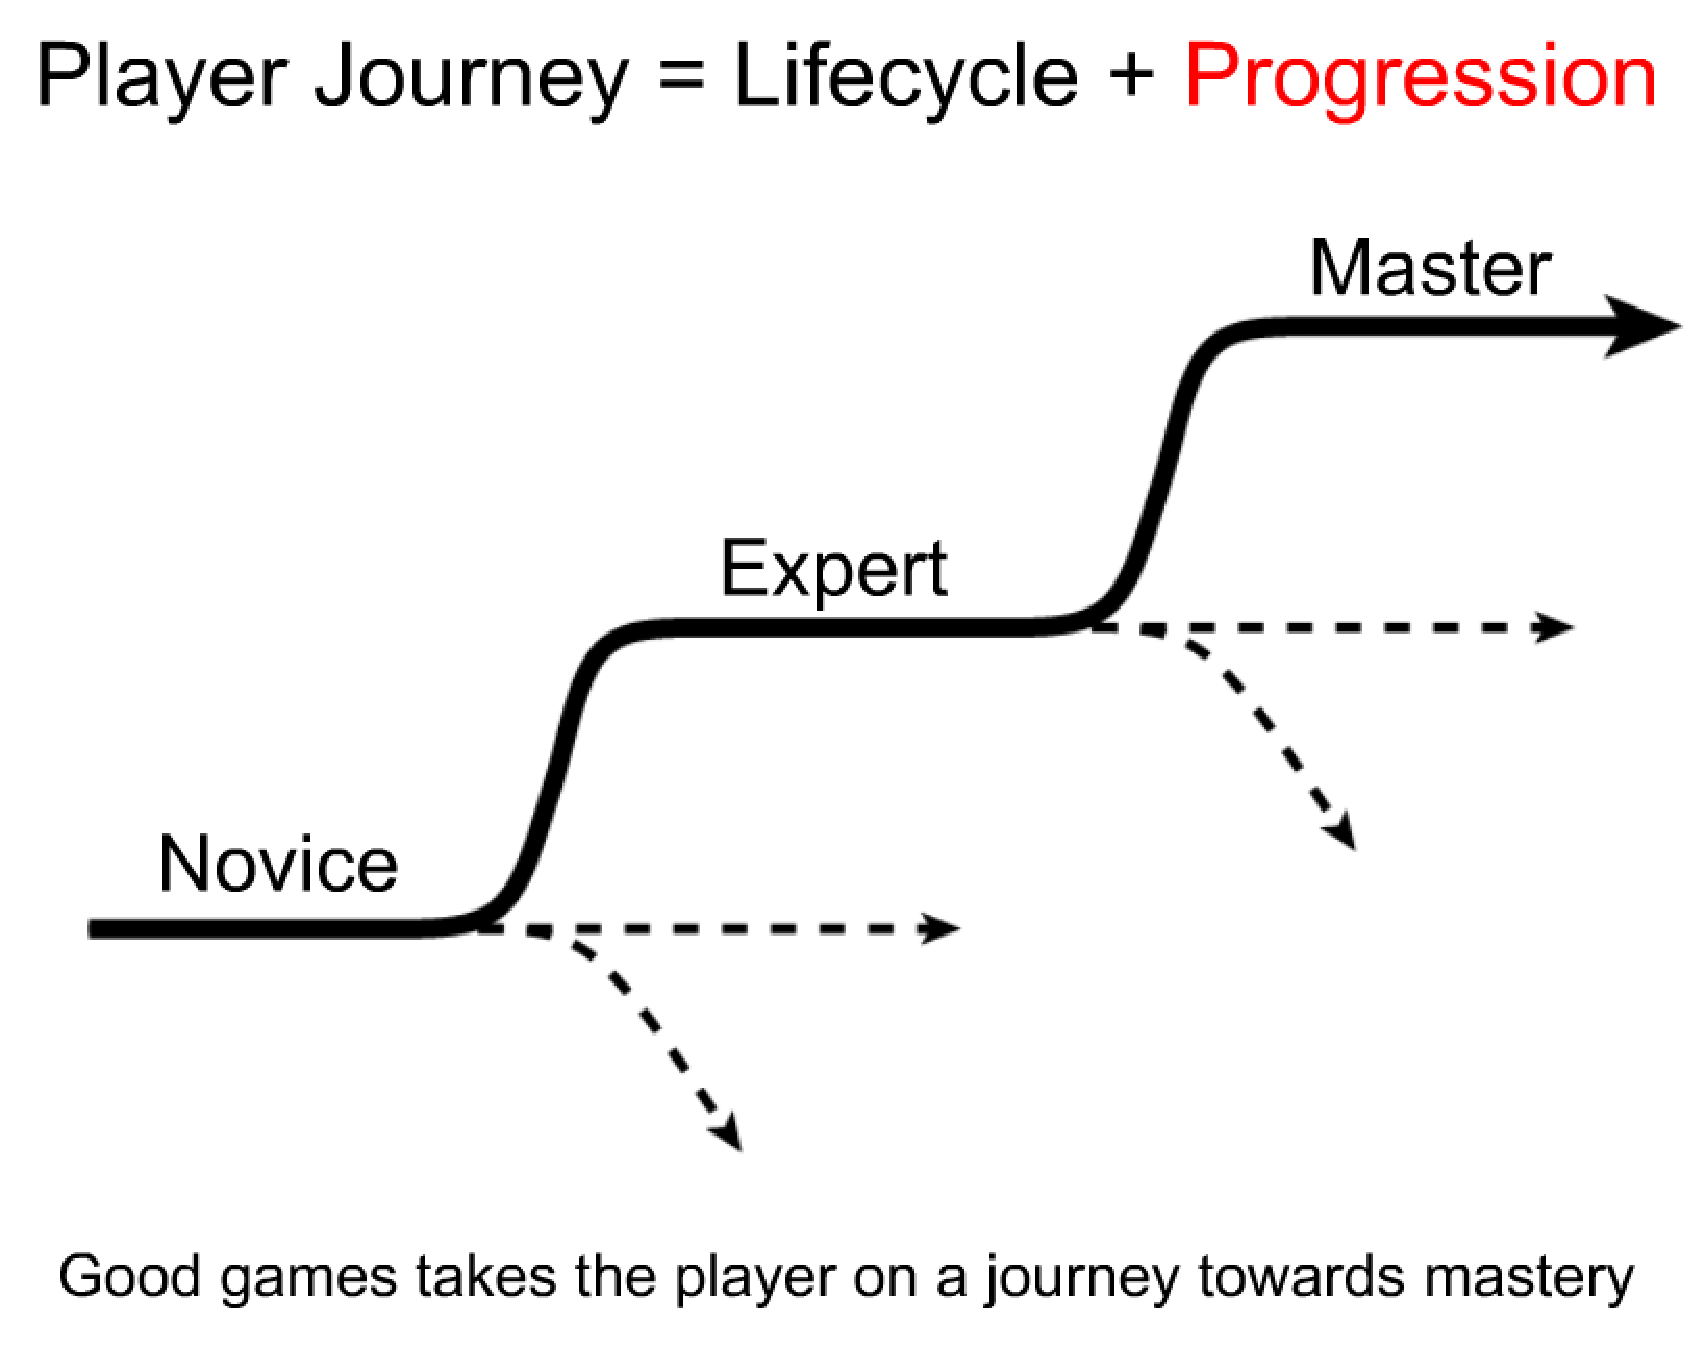
\includegraphics[height=2.1in]{kim-workshop.eps}}
		\subfigure[Game Design]{\label{fig:game-design}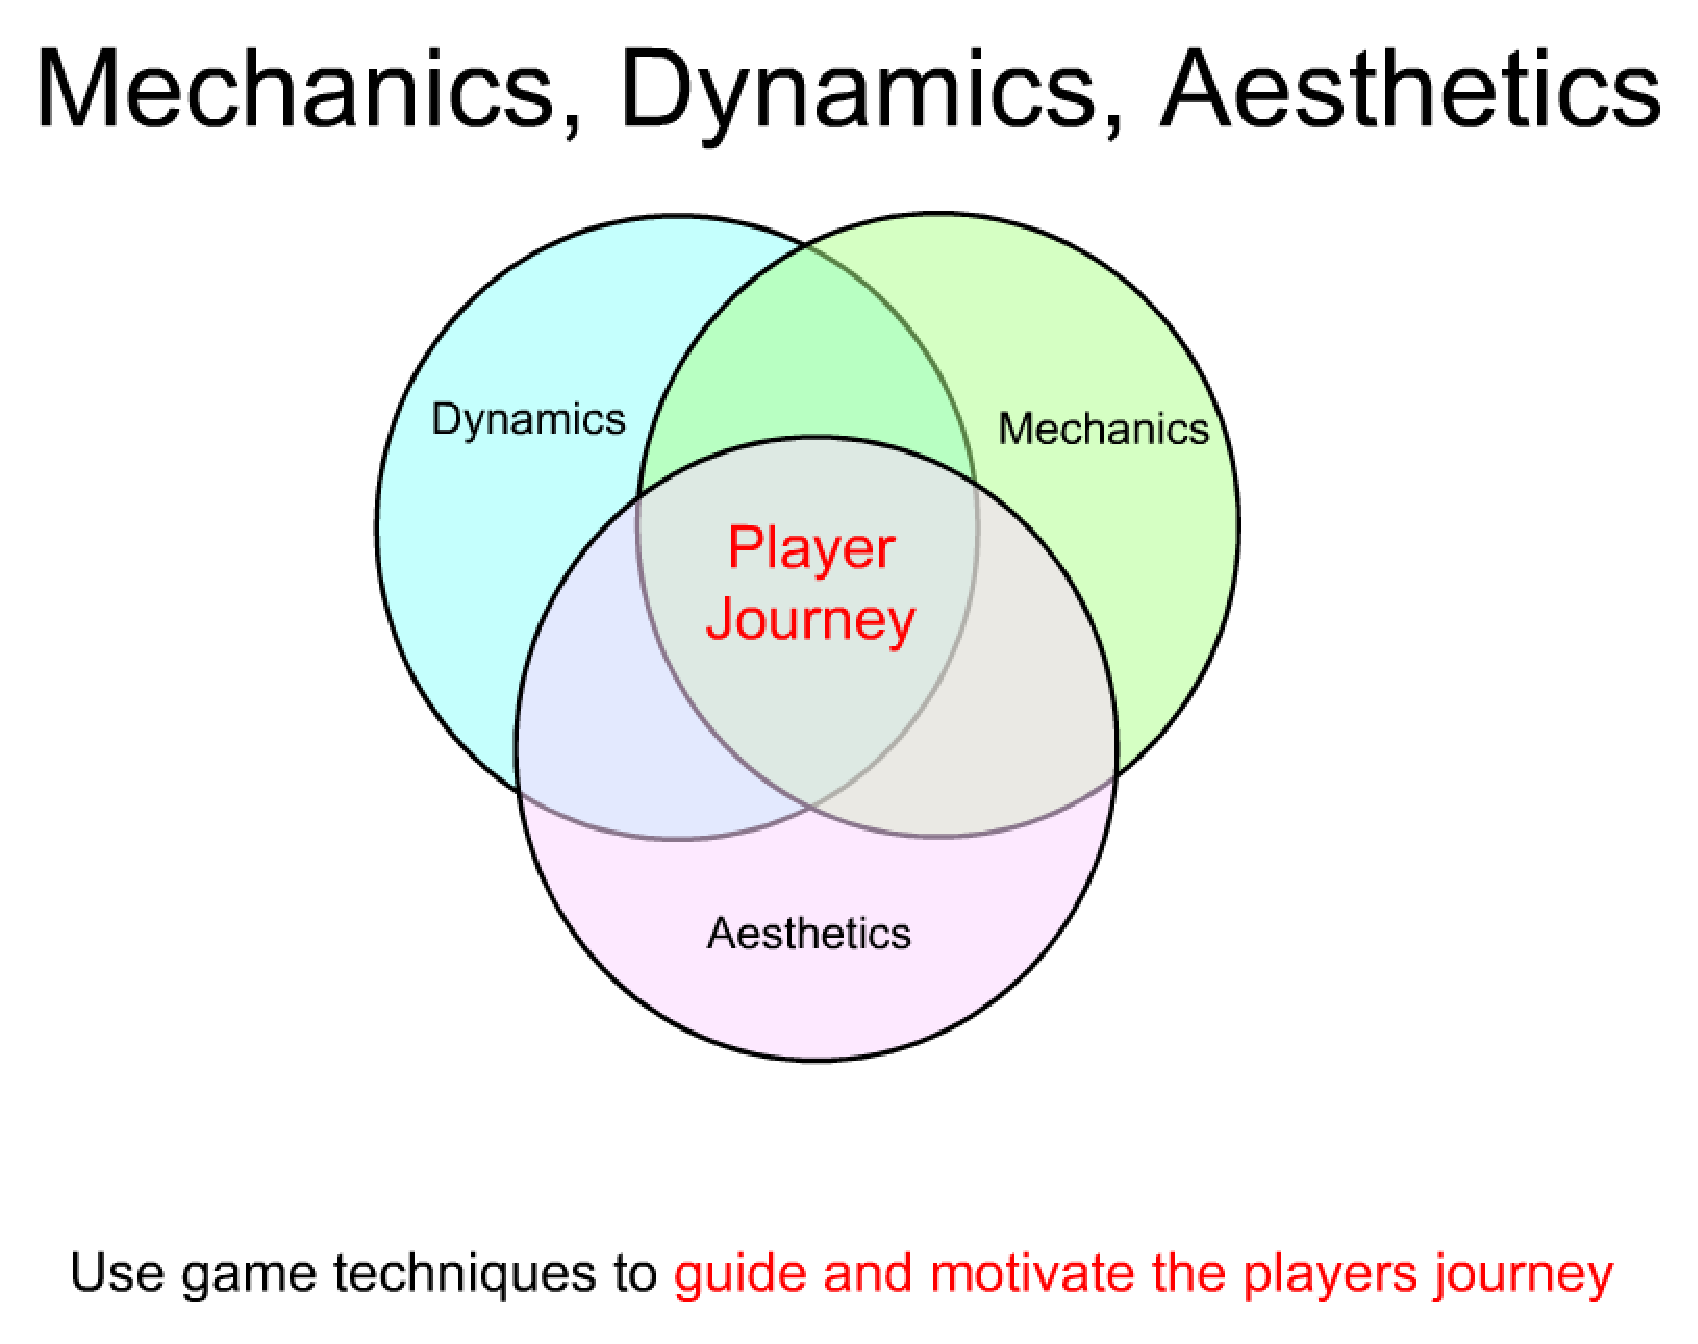
\includegraphics[height=2.1in]{kim-workshop2.eps}}
		\caption{Designing Player Journey (source: Kim \cite {Kim2010})}
		\label{fig:design-player-journey}
\end{figure}

Similarly, Sebastian Deterding not only criticized the current practice of simple gamification practices but stressed the important of ``meaningful play'' and proposed a user experience design around the three most important aspects: Meaning, Master and Autonomy \cite {Deterding2011meaningful}, It is an adaptation to the three elements to motivate people in Daniel Pink's book ``Drive: The Surprising Truth About What Motivates Us" \cite {pink2009drive}. Deterding explained that the reason why we play is because of the meaning and autonomy (choices) in the game. The mastery in the game give us fun and enjoyment.

The design of Makahiki is influenced by the above game design thinking. It combines extrinsic rewards such as prizes and achievement badges with the intrinsic motivation such as improving our environments by learning. Makahiki employs Kim's player journey idea \cite{Kim2010} to design the on-boarding and progression of levels in the smart grid game. Other game mechanics, such as the ``appointment mechanics'' and the ``social interaction'' described in SCVNGR's game dynamics play deck\cite{Biggs2010} are being used in Makahiki to improve player engagement. 

\section{Serious Games for Sustainability}
\label{sec:rel-sg-sustainability}

Makahiki is a framework for sustainability games. Serious games for sustainability are games designed to achieve the goal of sustainability development.    

Vermontivate \cite{vermontivate}, a type of community sustainability game, shown in \autoref{fig:vermontivate}, is similar to the games created by Makahiki.  Vermontivate is a team-based game where  the players compete to accrue as many points as possible for their towns or schools by participating in a variety of sustainability-focused actions. It runs for six weeks with mainly the participants in the state of Vermont. Because of the difference between the team size, team scores are calculated ``per-capita'' by adding up a team's total points and dividing by its number of players. A new set of challenges is announced every week with a different theme such as team-building, food, energy, transportation, capital, and future action. According to the initial sponsor of the game, Vermont Energy Investment Corporation, the first Vermontivate game began in May of 2012 and attracted 225 players from 31 Vermont towns. 95\% of players reported average to above-average understanding and engagement with climate change and sustainability after playing Vermontivate, compared to 78\% prior to playing \cite{veic}. Unlike Makahiki, Vermontivate game does not have individual points or prizes and more focus on activities and relies on self-reported participation. 

\begin{figure}[ht!]
	\centering
		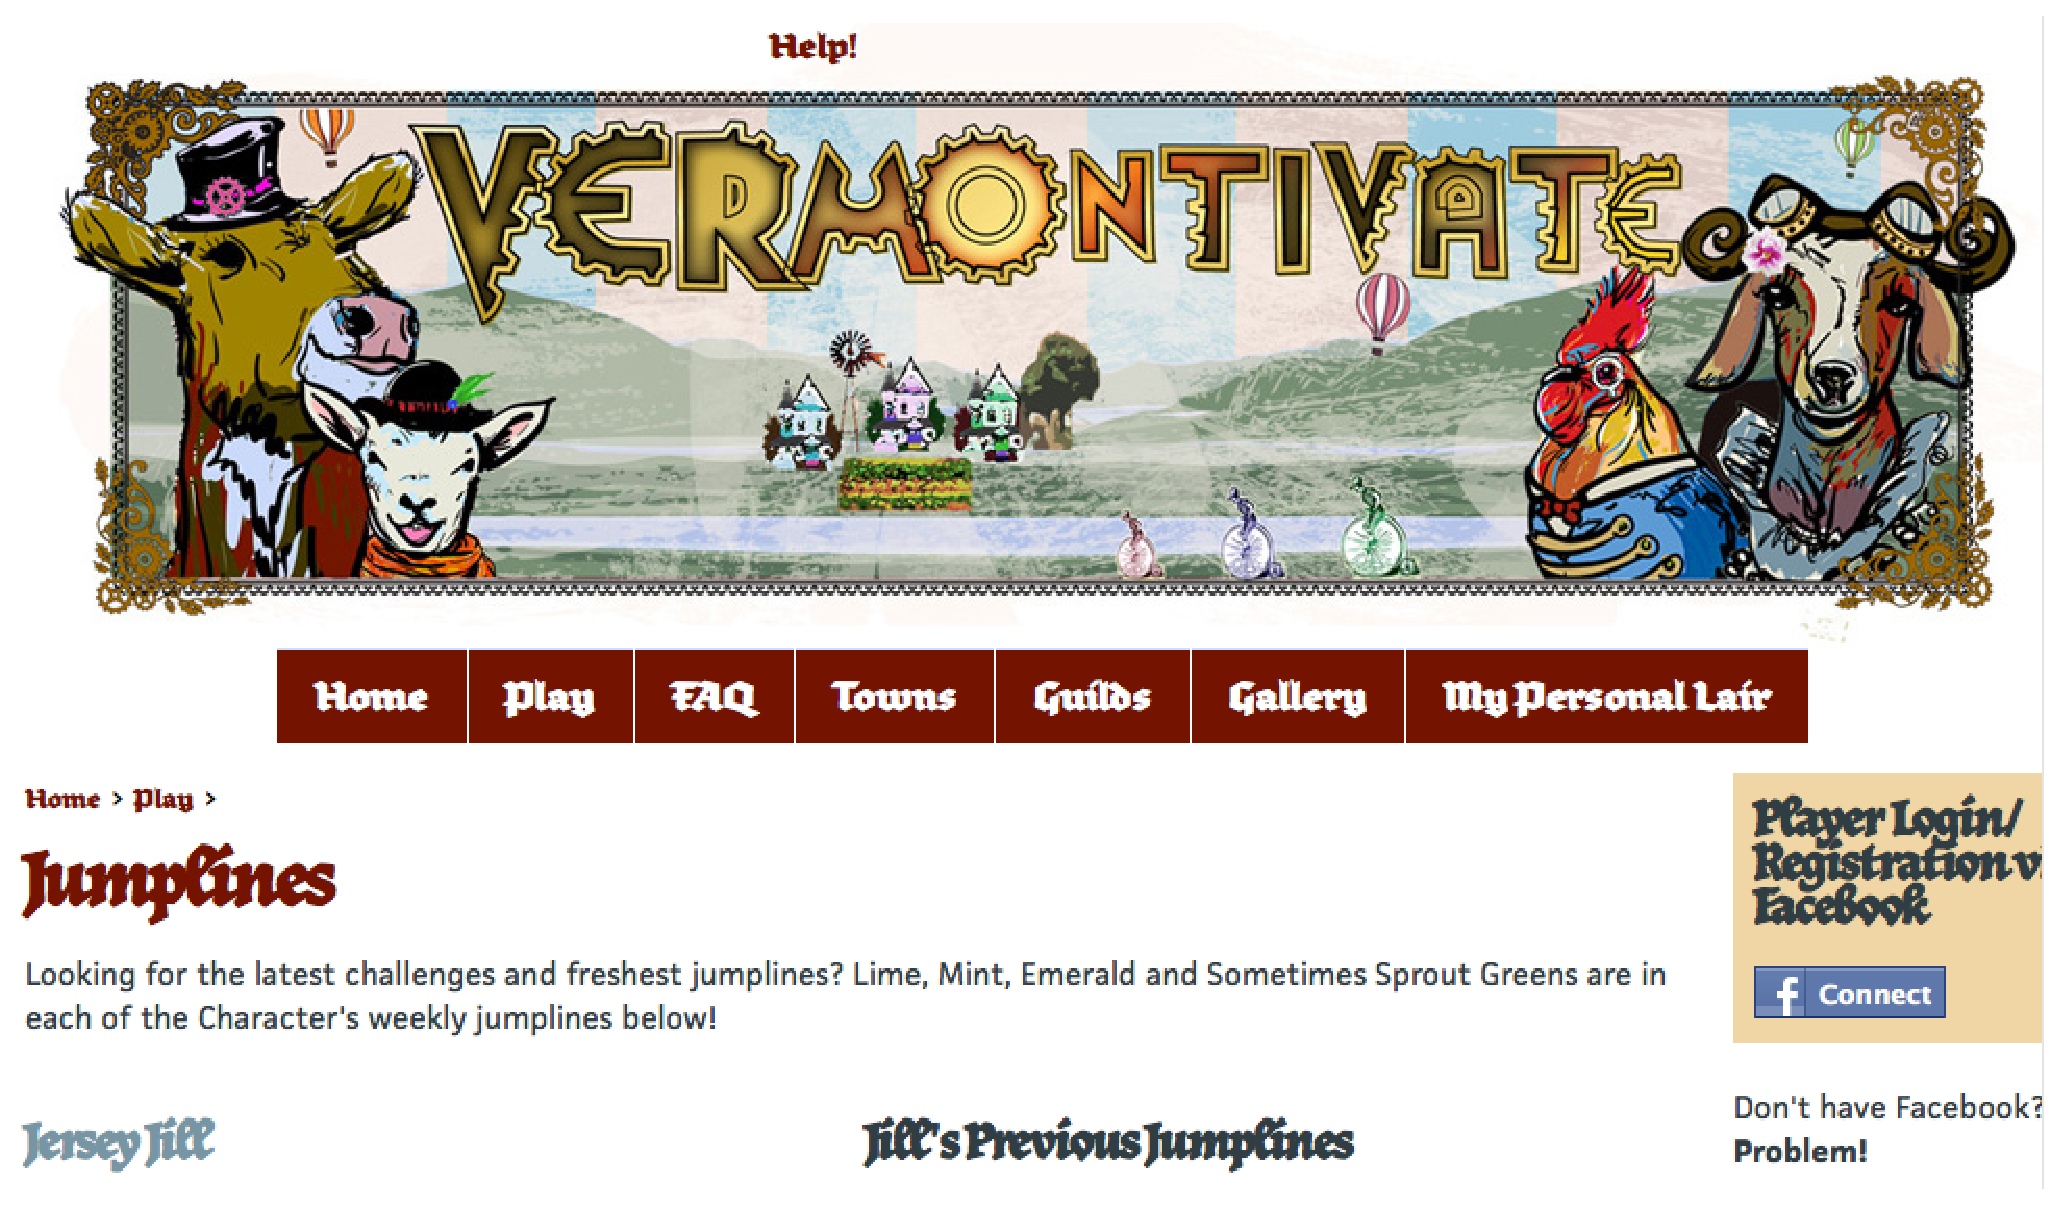
\includegraphics[width=0.6\columnwidth]{vermontivate}
		\caption{Vermontivate Sustainability Game (source: Vermontivate \cite{vermontivate})}
		\label{fig:vermontivate}
\end{figure}

Similar to Vermontivate, RecycleBank's ``Green Challenges'' \cite {recyclebank} is another serious game that used online gaming techniques to motivate participants to learn about green living and to take small green actions to live more sustainable lives offline. Figure \autoref{fig:RecycleBank1} shows a web page from the ``Green your home Challenge'' game. According to the ``Gaming For Good'' report \cite {gamingforgood}, 49,000 individuals participated in the ``Green Your Home Challenges''. Figure \autoref{fig:RecycleBank2} shows a section of the survey results regarding the self-reported sustainability behavior changes after the game. Partnered with Google Analytics and ROI research, they found that:
\begin{itemize}
	\item Gamification can increase awareness of positive environmental actions. 97\% of participants surveyed said the game increased their knowledge of the environment.
	\item Games can drive individuals to take positive social and environmental actions. Most participants surveyed indicated they are very or extremely likely to take green actions as a result of participating in the challenge.
	\item Games are an effective and appealing educational tool. 86\% participants agreed online games and contest can be a good way to inform and educate them personally.
\end{itemize}

\begin{figure}[ht!]
	\centering
		\subfigure[Green Your Home Challenge]{\label{fig:RecycleBank1}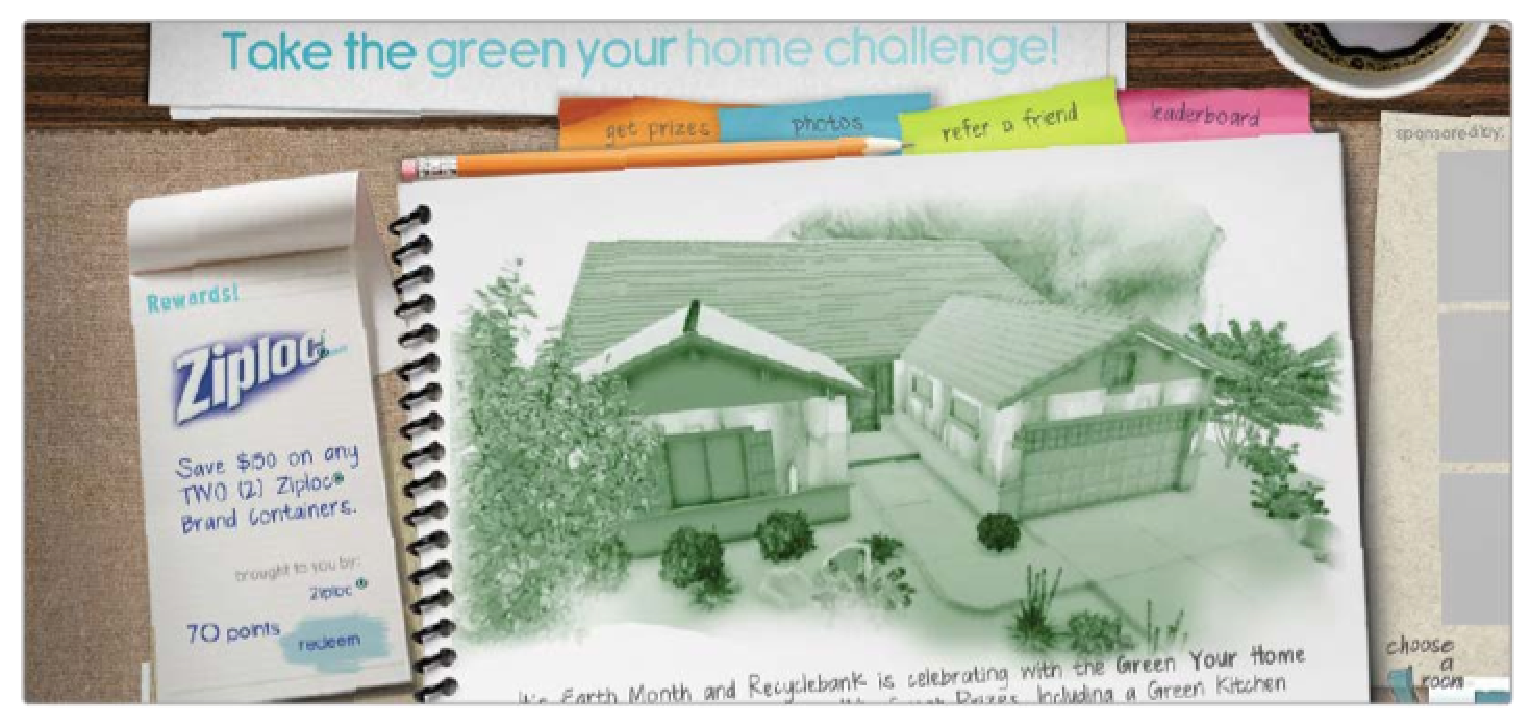
\includegraphics[width=0.6\columnwidth]{recyclebank1.eps}}
		\subfigure[Game Change Behavior]{\label{fig:RecycleBank2}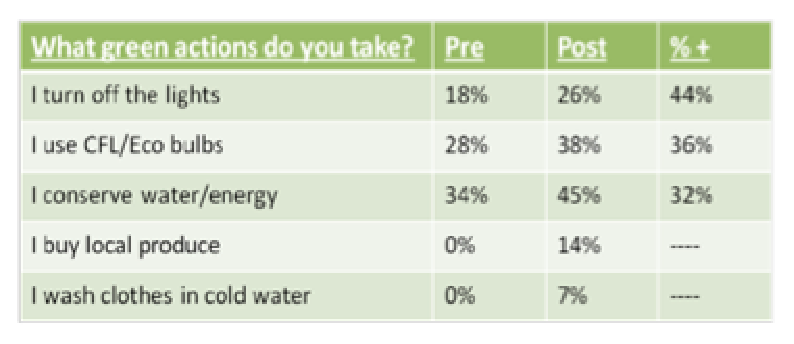
\includegraphics[width=0.6\columnwidth]{recyclebank2.eps}}
		\caption{RecycleBank - Gaming for Good}
		\label{fig:recyclebank}
\end{figure}

The Opower Social Energy Application \cite{opower} is another kind of sustainability serious game, available as a Facebook app on both web and smartphones. It is developed in partnership with Facebook and the Natural Resources Defense Council (NRDC) with the intention of making saving energy social \cite{alliance}. \autoref{fig:opower} shows a screenshot of the game. Through the app, participants can compare their energy use to similar homes, share energy saving tips, compete with friends, and participate in team-related energy reduction challenges. The app lowers the adoption barrier by directly importing the energy usage data from Opower utility accounts. If the participant does not have an Opower utility account, he can enter data manually from his utility bills, which requires more efforts and motivation to participate. Compared to Makahiki, the energy usage feedback from Opower is not real-time (monthly), and the home energy saving tips or recommendations are not linked to points, badges, or other virtual or real rewards.

\begin{figure}[ht!]
	\centering
		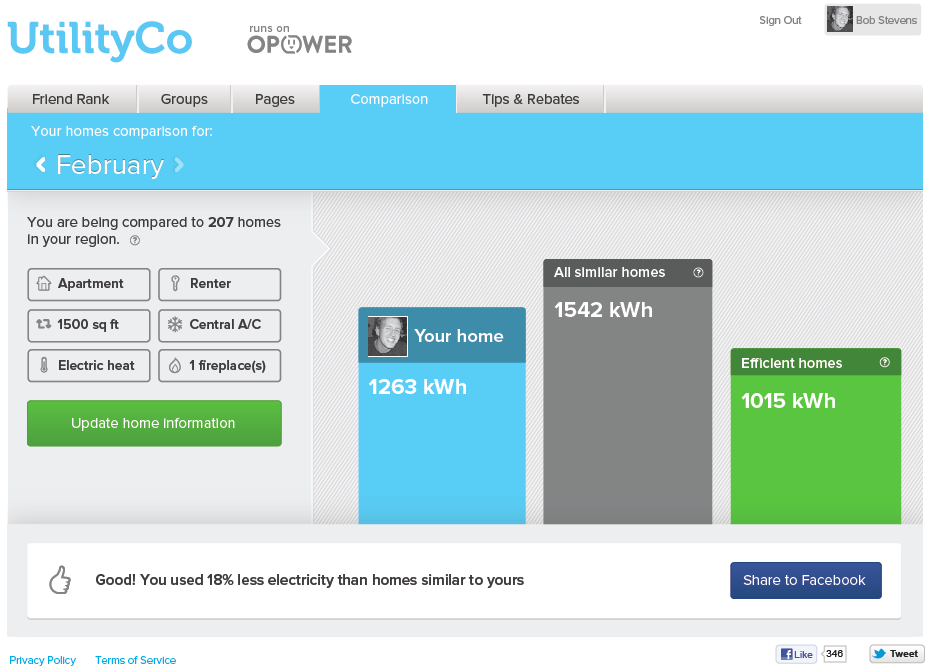
\includegraphics[width=0.6\columnwidth]{opower}
		\caption{Social Energy Application Engaging Consumers (source: Opower \cite{opower})}
		\label{fig:opower}
\end{figure}

Reeves et al. \cite{Reeves2011powerhouse} described the design of Power House, an energy game that connects home smart meters to an online multiple player game with the goal of improving home energy behavior. In the game, real world energy data is transformed into a ``more palatable and relevant form of
feedback'', and players may be incentivized by the in-game rewards to complete more energy-friendly real-world behaviors. \autoref{fig:powerhouse} shows a screenshot of the PowerHouse game. The games created by Makahiki share the similarity with PowerHouse in the way of providing real-time energy feedback to the player. Makahiki has more educational activities and less simulation game play than in PowerHouse.

\begin{figure}[ht!]
	\centering
		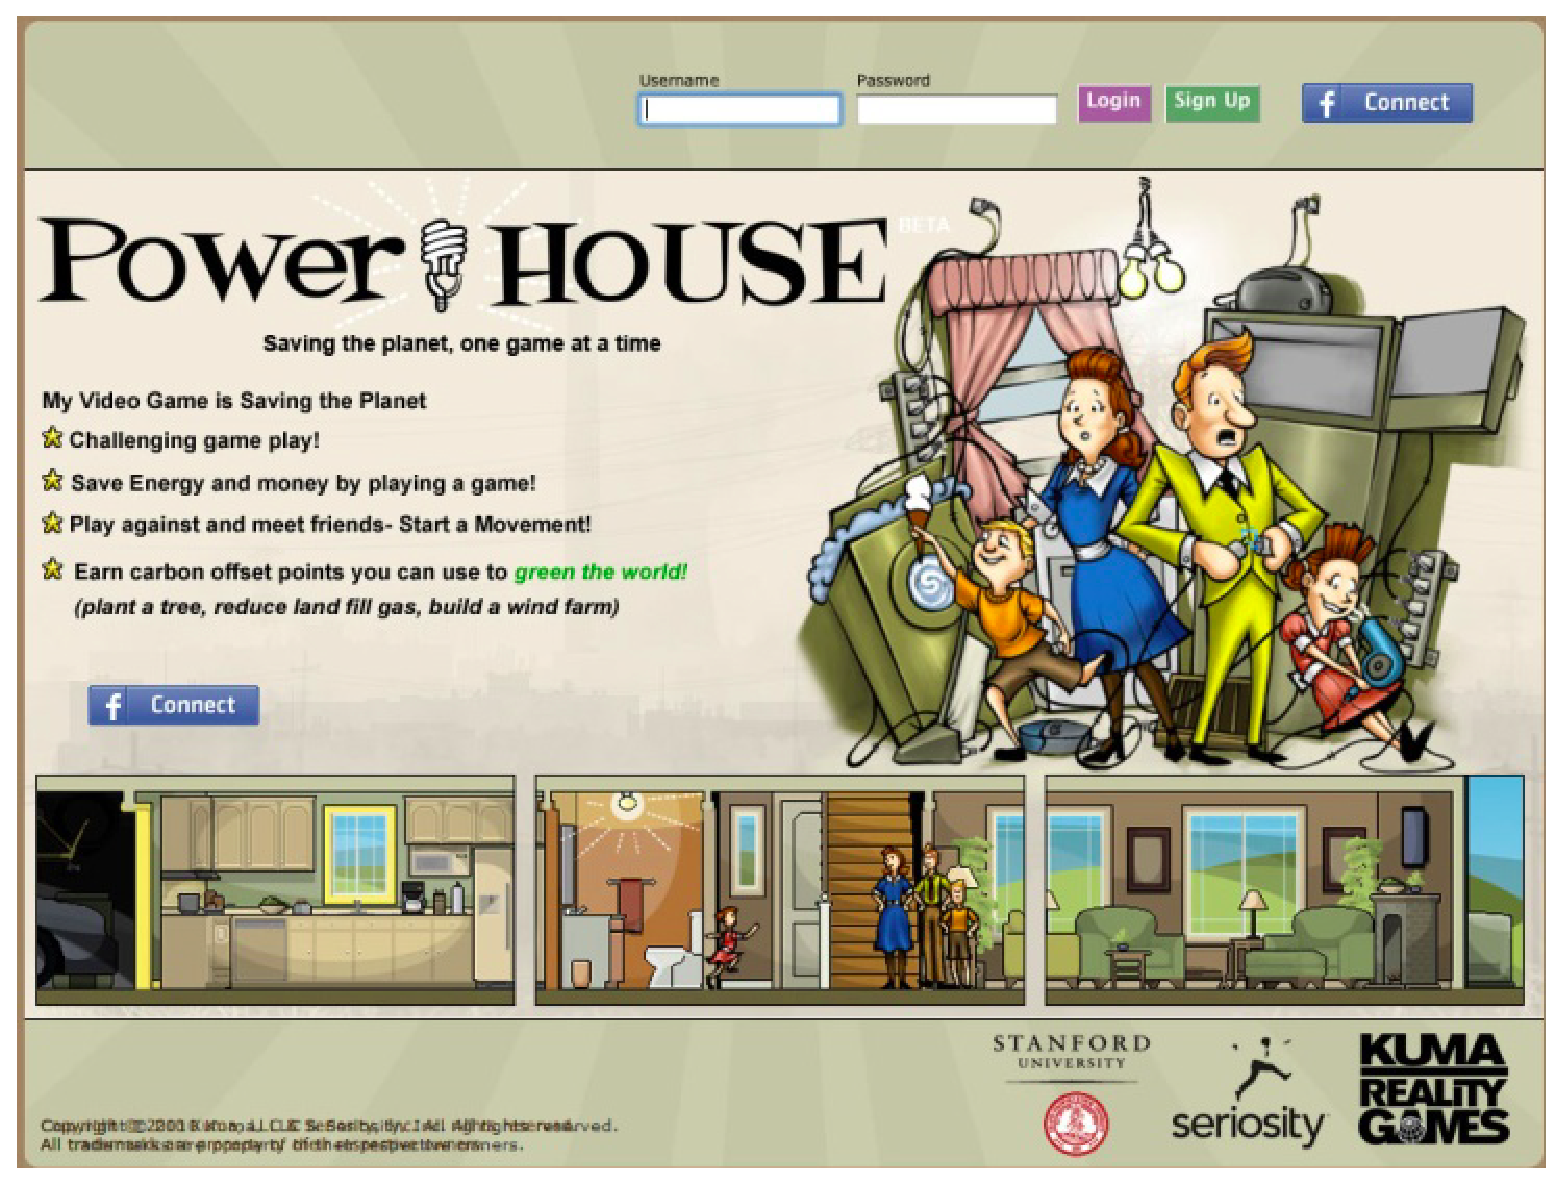
\includegraphics[width=0.6\columnwidth]{powerhouse.eps}
		\caption{Power House Game to Save Energy(source: Reeves \cite{Reeves2011powerhouse})}
		\label{fig:powerhouse}
\end{figure}

Another simulation based sustainability game worth of mention is the EnerCities \cite{enercities} developed by Dutch game developer Paladin Studios with a �1.4M budget funded by the European Commission. Awarded the title of ``Best Learning Game 2010'', offered an online learning game for young people (typical target group: 15-20 years old) to experience energy-related implications. The goal of the game is to create and expand virtual cities dealing with pollution, energy shortages, renewable energy etc. Available both as  a standalone website and on Facebook, The game was played by thousands of students from more than 110 schools across Europe. The game offers a semi-realistic simulation with cartoony 3D (via Unity3D plug-in\cite{unity3dplugin}) visual styles with multiple level game play. \autoref{fig:enercities} shows a screenshot of the game. Similar to PowerHouse game, EnerCities game engages player via the graphical simulation of the energy related issues. The player experience is more video game like than the other sustainability games such as the one's create by Makahiki. On the other hand, Makahiki as a extensible and configurable game framework, it is possible to include some simulation games such as EnerCities and PowerHouse inside Makahiki to provide better player experience and engagement.

\begin{figure}[ht!]
	\centering
		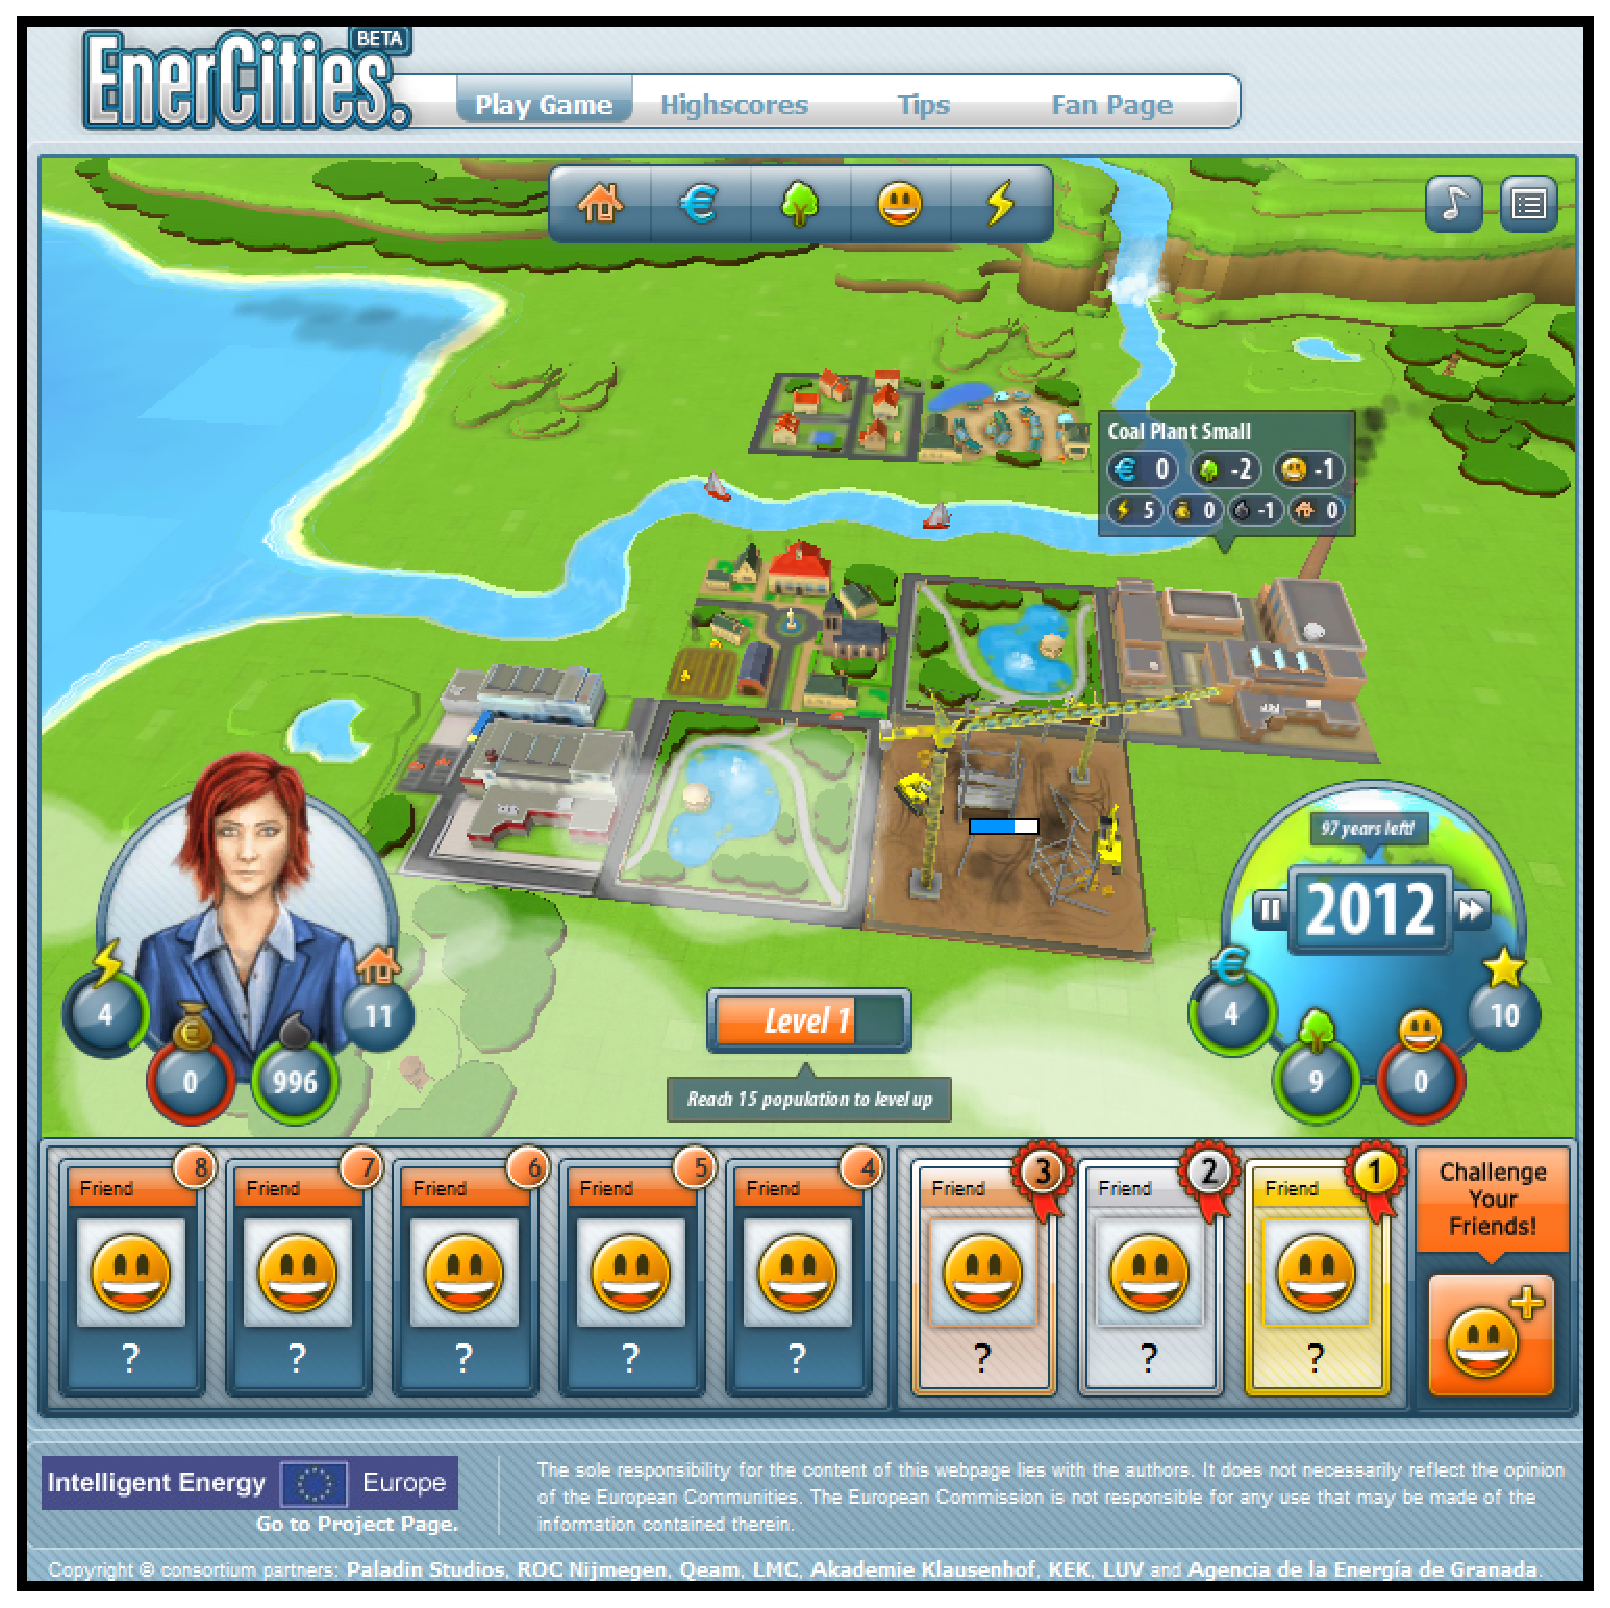
\includegraphics[width=0.6\columnwidth]{enercities}
		\caption{EnerCities - simulation based sustainability game(source: EnerCities \cite{enercities})}
		\label{fig:enercities}
\end{figure}

\autoref{table:sustainability-games} summaries the above serious games for sustainability and compares to the games created by Makahiki.

\begin{table}[ht!]
  \centering
        \begin{tabular}{| p{2.1cm} | p{2.4cm} | p{2.9cm} | P{1.5cm} | p{2cm} | c |} 
        \hline
      \tabhead{Game} & \tabhead{Type} & \tabhead{Targeted player} & \tabhead{Reward} & \tabhead{Competition} & \tabhead{Mobile} \\
        \hline
        Vermontivate 	& Website 		& Community	& Prizes & Team 	& \checkmark \\
        RecycleBank  	& Website 		& Community	& Prizes & Team	& \xmark \\
        Opower     	& Facebook App 	& Energy consumer & Virtual & Individual  & \checkmark \\
        PowerHouse     	& 2D Simulation 	& Energy consumer & Virtual & Individual  & \xmark \\
        EnerCities	    	& 3D Simulation 	& Schools & Virtual	& Individual  & \xmark \\
	Makahiki		& Website		& Schools & Prizes \& virtual & Team \& individual  & \checkmark \\
        \hline
        \end{tabular}
        \caption{Serious games for sustainability}
        \label{table:sustainability-games}
\end{table}

\section{Serious Game Frameworks}
\label{sec:rel-sg-framework}

Game frameworks (also known as game engines) \cite{sherrod2006ultimate} are ``comprised of a collection of different tools, utilities, and interfaces that hide the low-level details of the various tasks that make up a game''. Examples of game frameworks include:
\begin {itemize}
    \item Unreal \cite{unrealengine}:  The Unreal Engine is a game engine developed by Epic Games, it is primarily used in first person shooter games, providing tools and building blocks for 3D rendering, collision detection, AI, networking etc.
    \item PapayaMobile \cite{papayamobile}: PapayaMobile is a free cross platform social game engine on Android and iOS platform. It provides an SDK and a platform for mobile game developers to create and release games in a ``user-friendly, straightforward way''.
    \item OpenLabyrinth \cite{openlabyrinth}: OpenLabyrinth is an open source game framework that allows its users to create, run and analyze a wide range of different pathway-based activities for healthcare education.
    \item Fabula \cite{fabula}: Fabula is an open source Python game engine for adventure, role-playing and strategy games and digital interactive storytelling. It provides a library and game world abstraction intuitive to people who have not been involved in game development before and hide as much as low level technical details as much as possible.
\end {itemize}

One of the benefits of using a game framework is that, if correctly designed, it will provide useful and reusable ``building blocks'' with which to develop a variety of games. Similarly, serious game frameworks also provide building blocks that enable the serious game developer to focus more time and thought on content and results instead of on the technical details and infrastructure for creating the serious game.

There are two serious game frameworks related to sustainability development. One such framework is the Building Dashboard \cite{building-dashboard}, developed by Lucid Design Group, as shown in \autoref{fig:building-dashboard}.

\begin{figure}[ht!]
	\centering
		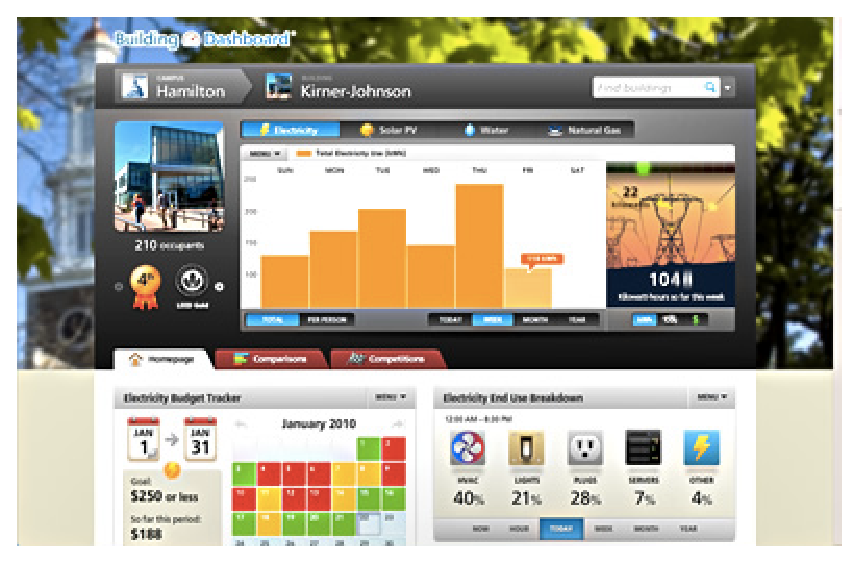
\includegraphics[width=0.6\columnwidth]{building-dashboard.eps}
		\caption{Building Dashboard (source: Lucid \cite{building-dashboard})}
		\label{fig:building-dashboard}
\end{figure}

Building Dashboard is commercial platform that ``enables energy reduction competition and empowers building occupants to become active participants in energy management''. It is used to support the Campus Conservation Nationals (CCN) \cite{competetoreduce}, a nationwide electricity and water use reduction competition on college campuses. In CCN 2014, the framework was used by 109 schools in North America to display the energy and water consumption of the competition participants. It enables viewing, comparing and sharing building energy
and water use information on the web through a visual interface.

Building Dashboard is similar to Makahiki that they are both frameworks for supporting sustainability competitions, but the
cost of Building Dashboard as a commercial system creates a barrier to wider adoption. In addition, the
Building Dashboard solution focuses on providing energy information as a passive media. Besides a scoreboard, there is little interaction between participants and the system. There are less game elements other than providing a scoreboard to display the ranking of the competing teams, moreover, there is no individual points or ranking. Unlike Makahiki, Building Dashboard does not have the concept of individual registered player account, thus it does not have the capability to provide the evidence of individual player engagement.

Another framework related to sustainability is the Stanford Energy Services Platform \cite{Armel-2012}, as shown in \autoref{fig:stanford-platform}. It provides services to support the creations of energy efficiency program and research. The services include data storage, a recommendation system, user registration and participation assignment, surveys and analytics. It had been utilized to support the implementation of several of Stanford's energy saving projects and energy related serious games, such as the Power House game, Power Down game, and Energy Calculator. At this point, there is not enough information about the Stanford Energy Services Platform regarding the availability and features. 

\begin{figure}[ht!]
	\centering
		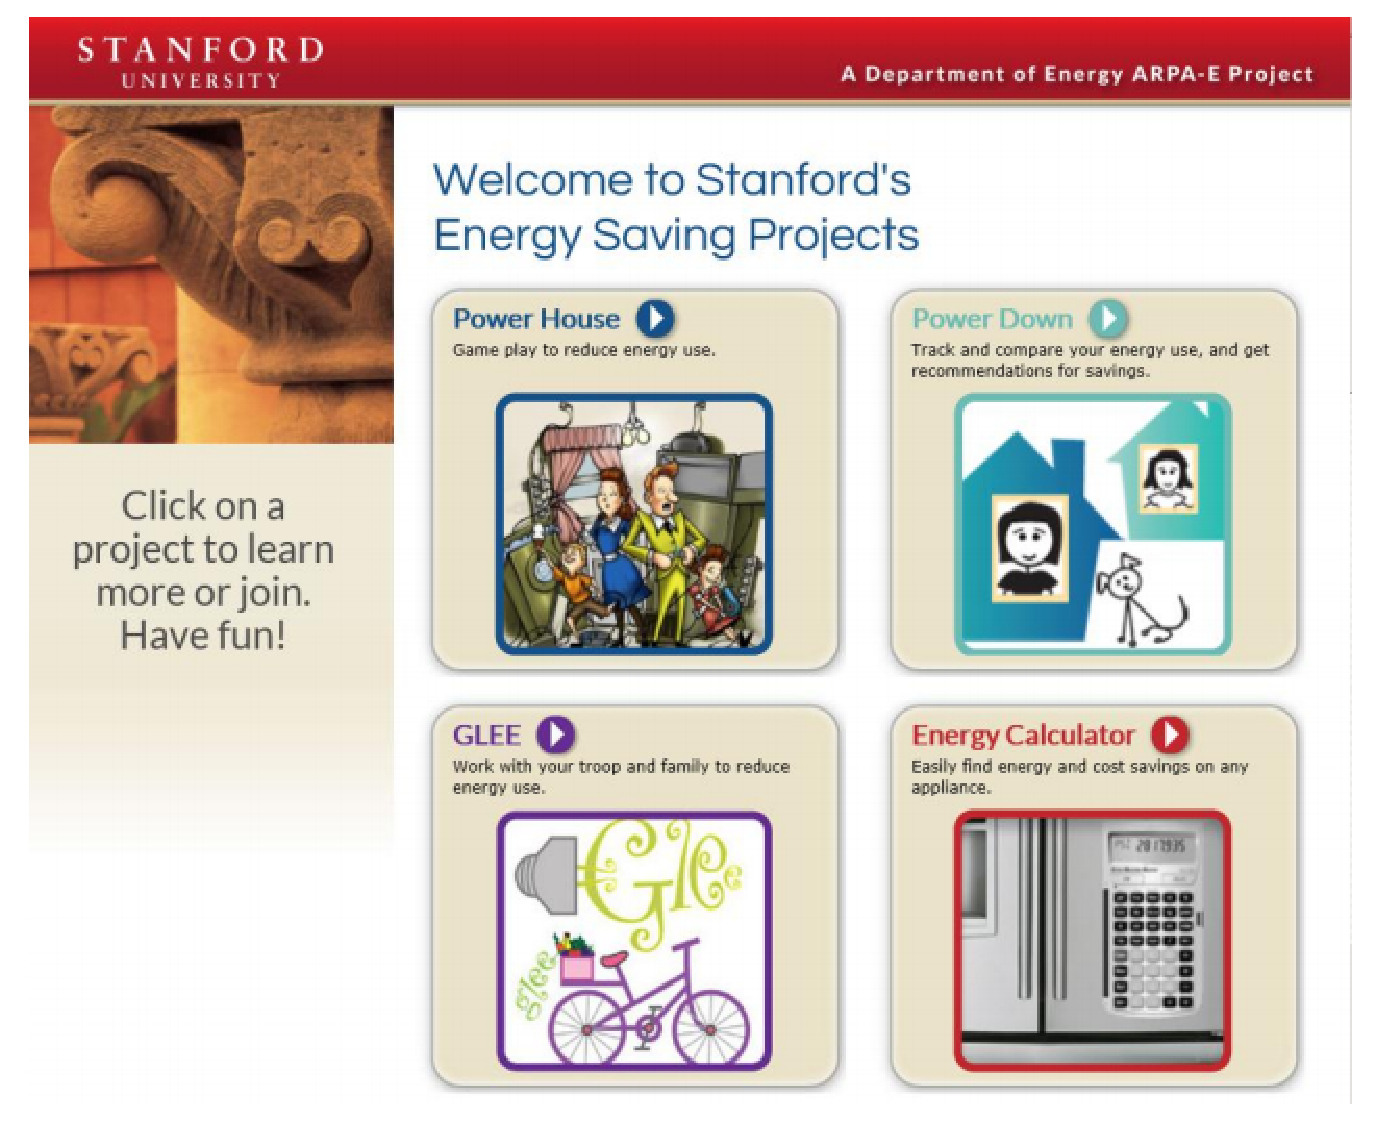
\includegraphics[width=0.6\columnwidth]{stanford-esp.eps}
		\caption{Stanford Energy Services Platform (source: Stanford \cite{Armel-2012})}
		\label{fig:stanford-platform}
\end{figure}
 
%% TODO: add non-serious game framework assessment
\section{Serious Game and Framework Assessment}
\label{sec:rel-sg-assessment}

This section examines the assessment of serious game frameworks. It starts by looking at the assessment of serious games, then  the assessment of game frameworks in general. From my literature search, I have not yet found any prior work concerning the comprehensive approach for the particular needs of a serious game framework assessment. Nevertheless the research in game and framework assessment methods provides ground works for the SGSEAM method that we designed for use in assessing a serious game framework.

\subsection{Serious Game Assessment}

In order to assess a serious game framework such as Makahiki, it is important to assess the serious games the framework produces.  One fundamental question in evaluating a serious game is the extent to which the
game achieves its ``serious'' purpose.  This is quite different from traditional entertainment games, in which evaluation focuses on usability or playability \cite{song2007new}. In the field of serious games, there is an increasing focus on the methodology of game evaluation \cite{Mayer2012233}. 

De Freitas and Oliver \cite{de2006can} point out that there are few frameworks to support the evaluation of education games. They introduce a four dimensional framework for evaluating 
educational games and simulations. The framework consists of: the context, the pedagogy, the representation, and the learner (or player). \autoref{fig:four-dimensional-framework} illustrates the evaluation framework.

\begin{figure}[ht!]
	\centering
		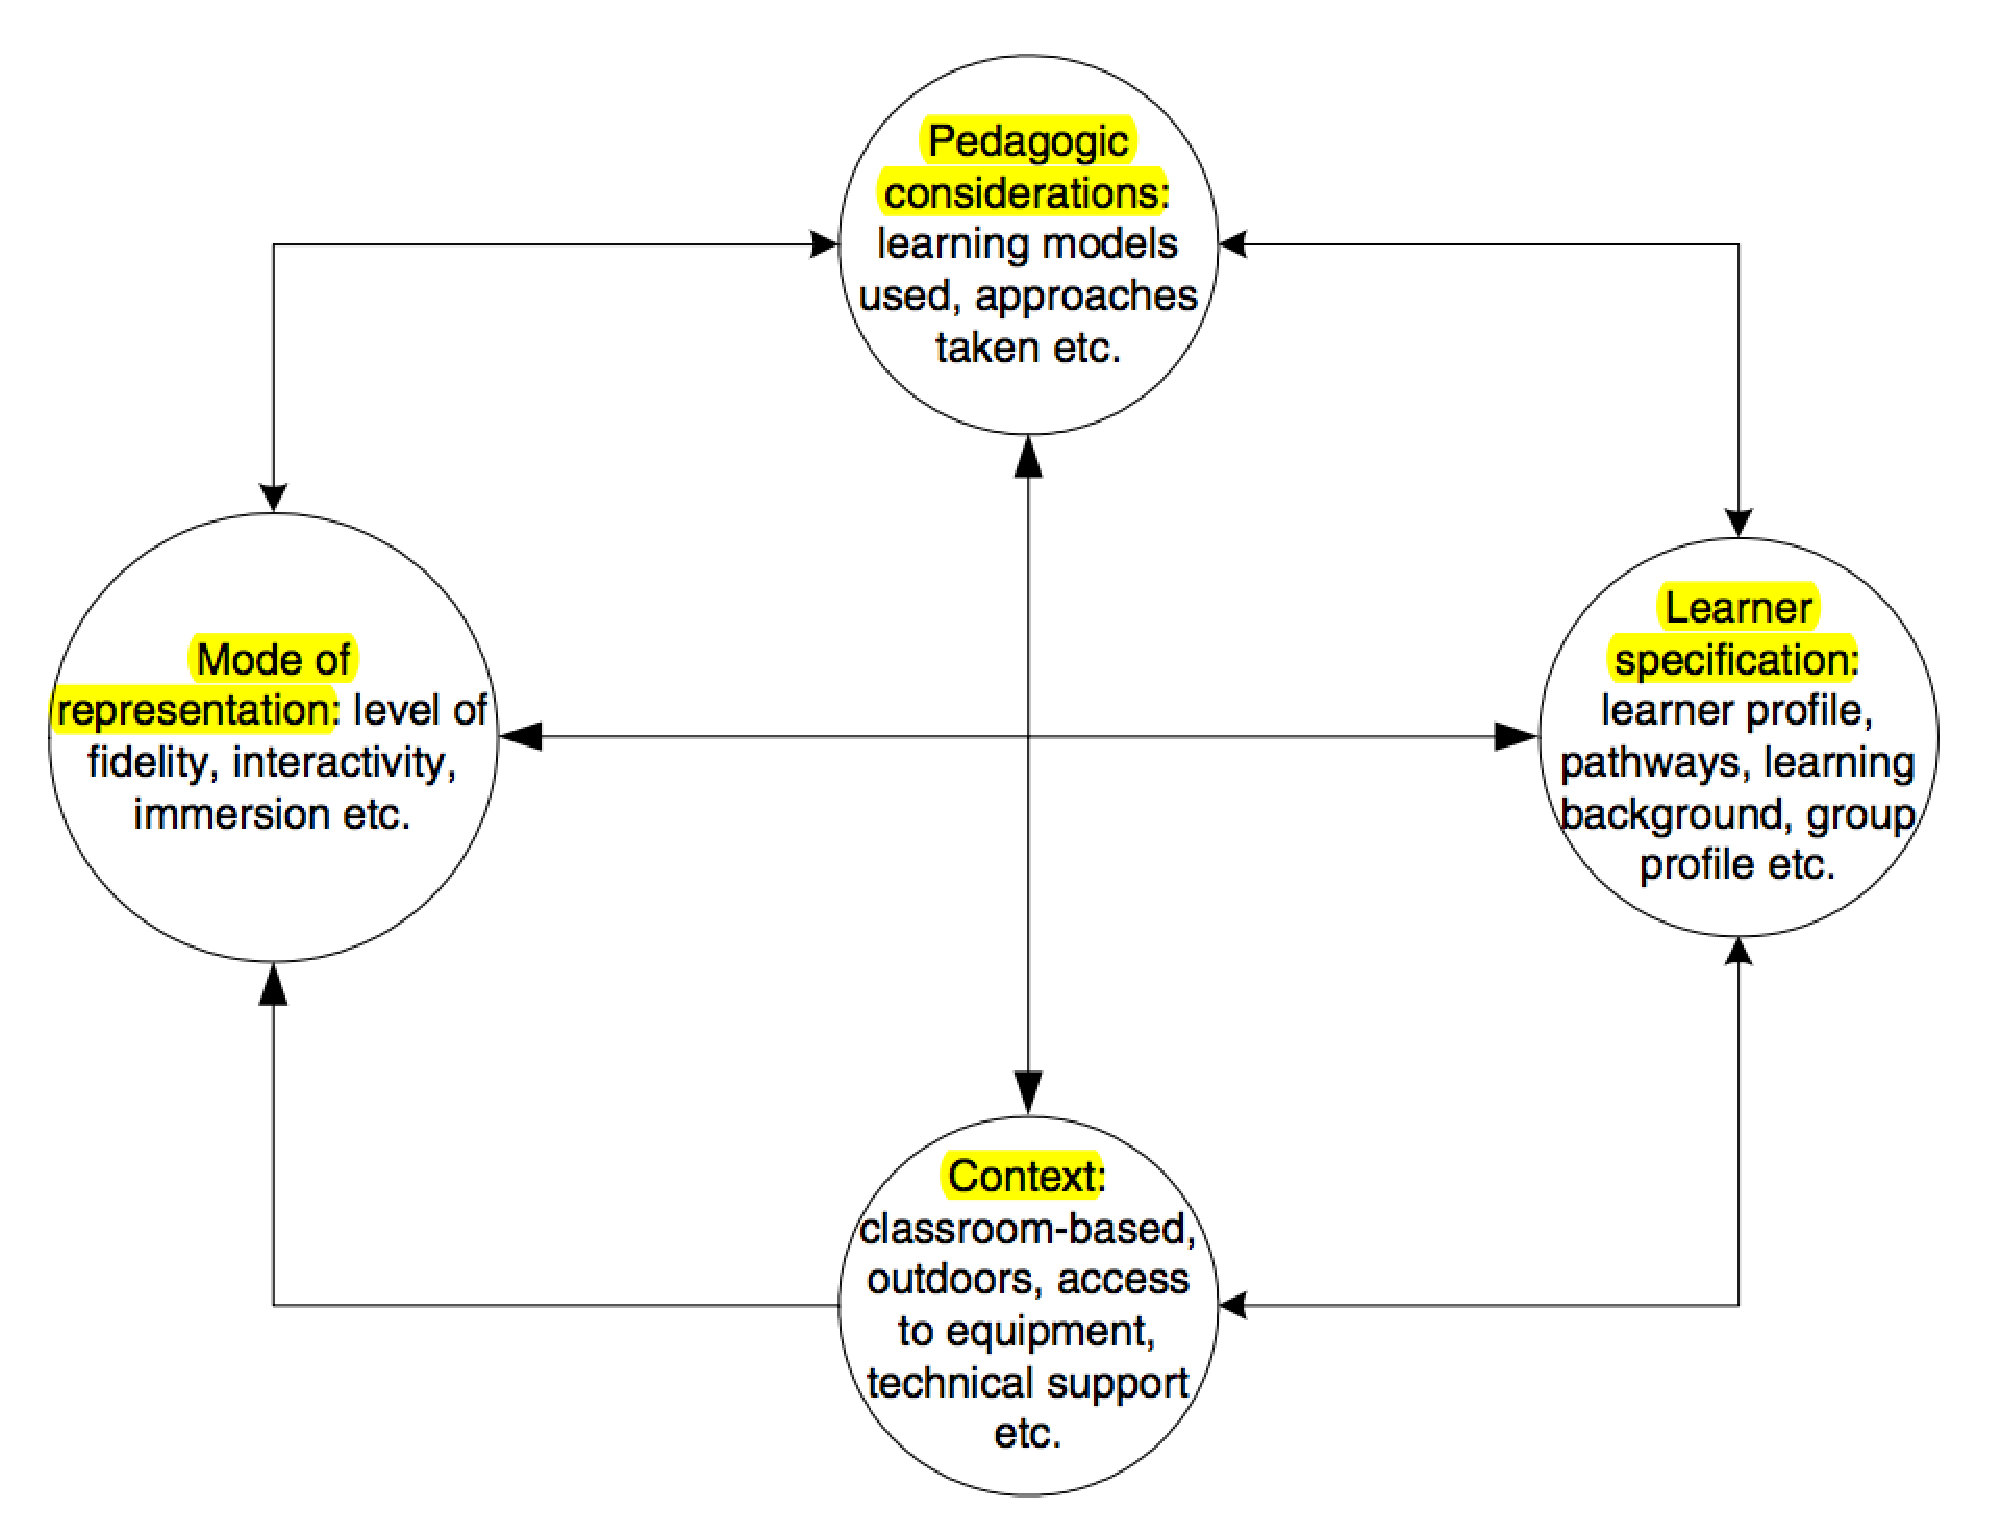
\includegraphics[width=0.6\columnwidth]{game-eval.eps}
		\caption{Four Dimensional Framework for Evaluating Educational Games \cite{de2006can}}
		\label{fig:four-dimensional-framework}
\end{figure}

Harteveld \cite{harteveld2010triadic} also agrees that ``Evaluatory research for games with a serious purpose is still at its infancy''. He proposes an evaluation framework called ``Triadic Game Evaluation (TGE)'' for assessing serious games. It consisting of three perspectives: Reality,
Meaning, and Play, as illustrated in the \autoref{fig:triadic-game-eval}.

\begin{figure}[ht!]
	\centering
		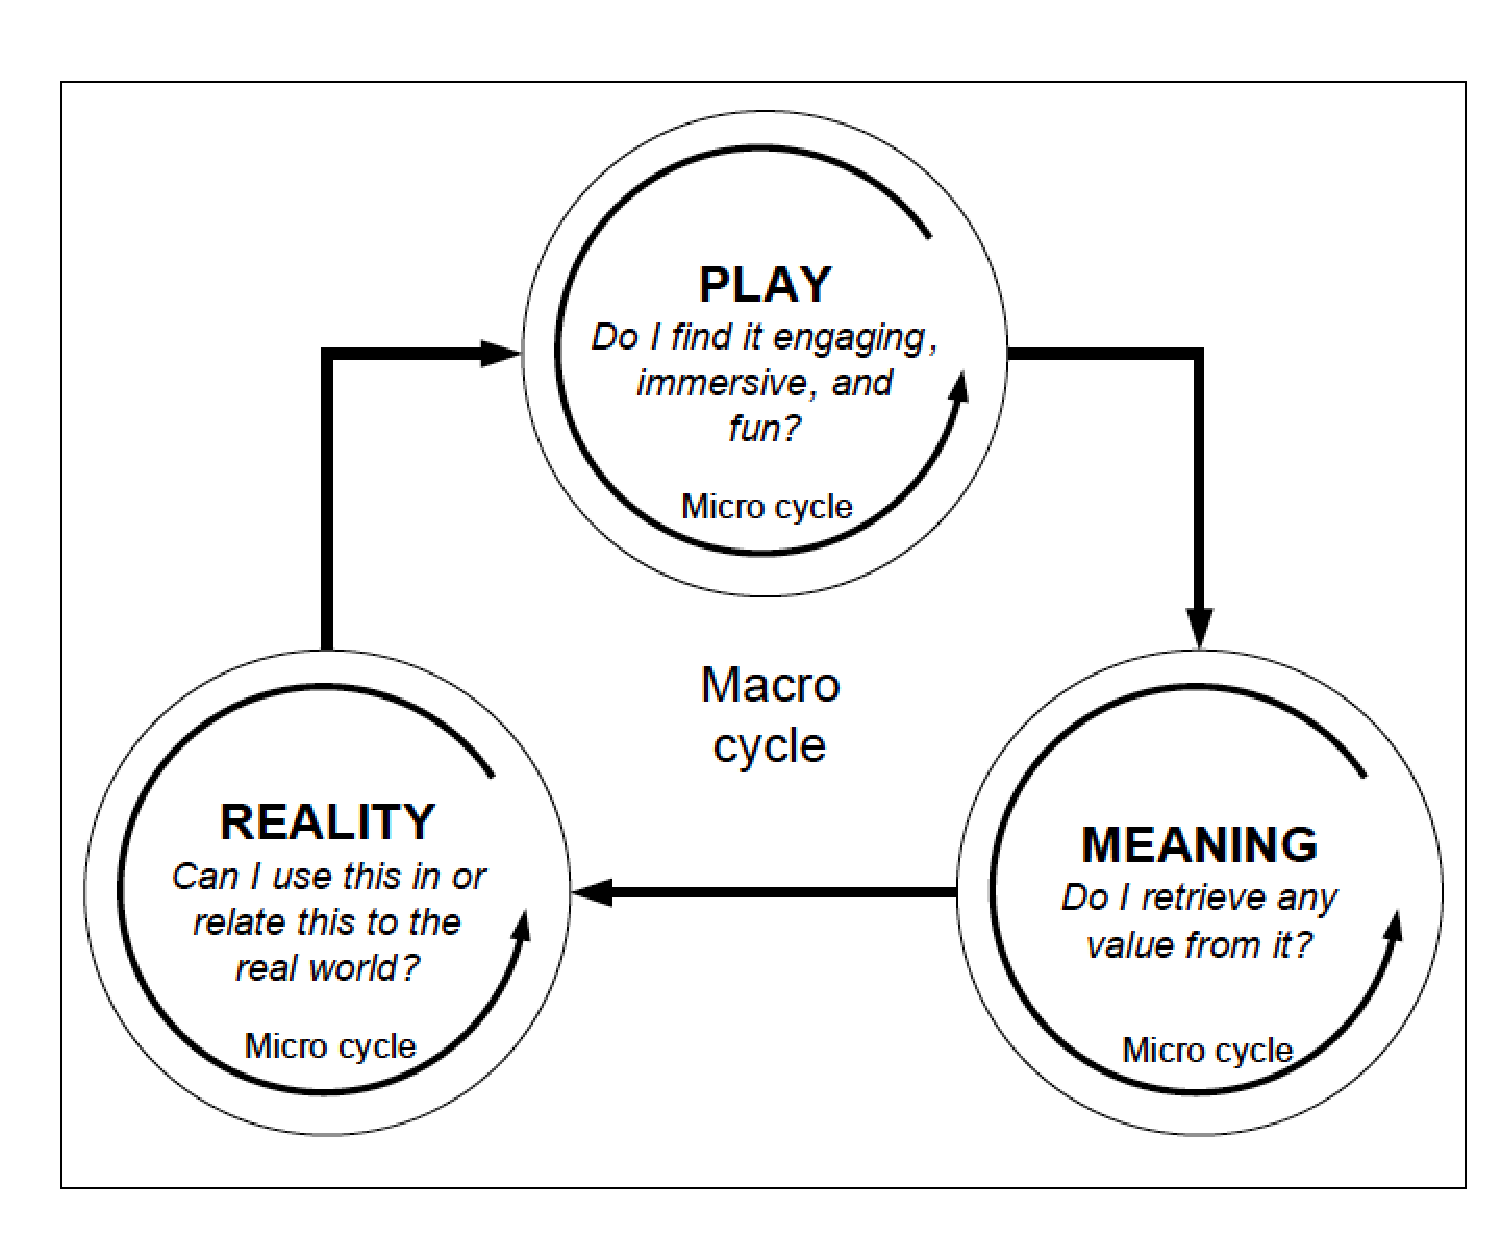
\includegraphics[width=0.6\columnwidth]{triadic-eval.eps}
		\caption{Triadic Game Evaluation (TGE) \cite{harteveld2010triadic}}
		\label{fig:triadic-game-eval}
\end{figure}

Effectiveness assessment is often part of the serious game evaluation. In their evaluation of the EnerCities game, Knol and Vries reported that they conducted a survey to test differences in awareness concerning energy-related issues between a group who had actually played the game and those who had not (between-participants design). Examples of the survey questionnaires include:
\begin{itemize}
\item What did you find out about energy saving and �green energy� after playing the game?
\item After playing the EnerCities game I was interested in learning more about energy saving and �green� energy
\item Playing the Enercities game has increased my concern about the environment
\item Playing the Enercities game made me aware of the linkages between economy, energy usage and environment
\item Playing the EnerCities game made me aware that I should lower my own energy usage
\end{itemize}

\subsection{Framework Assessment}

The above approaches focus on evaluation of a single game, as opposed to a game {\em
  framework}. One of the benefits of using a game framework is that, if correctly designed, it will provide useful and reusable ``building blocks'' with which to develop a variety of games. Yet how are we to know if a game framework has been ``correctly designed''?

Berger and Muller \cite {fabulaengine} describe their approach of using the Technology Acceptance Model (TAM) to evaluate the custom game engine Fabula \cite{fabula}. Technology Acceptance Model \cite {davis1986technology} is a well received theoretical model on assessing user acceptance of computer-based information systems, introduced by Fred Davis in his doctoral thesis in 1985. TAM considers that system use is a response that can be predicted by user motivation, which is influenced by an external stimulus of the system's features and capabilities. \autoref{fig:tam} illustrates the original Davis model. X1, X2 and X3 in the figure represent the system features.

\begin{figure}[ht!]
	\centering
		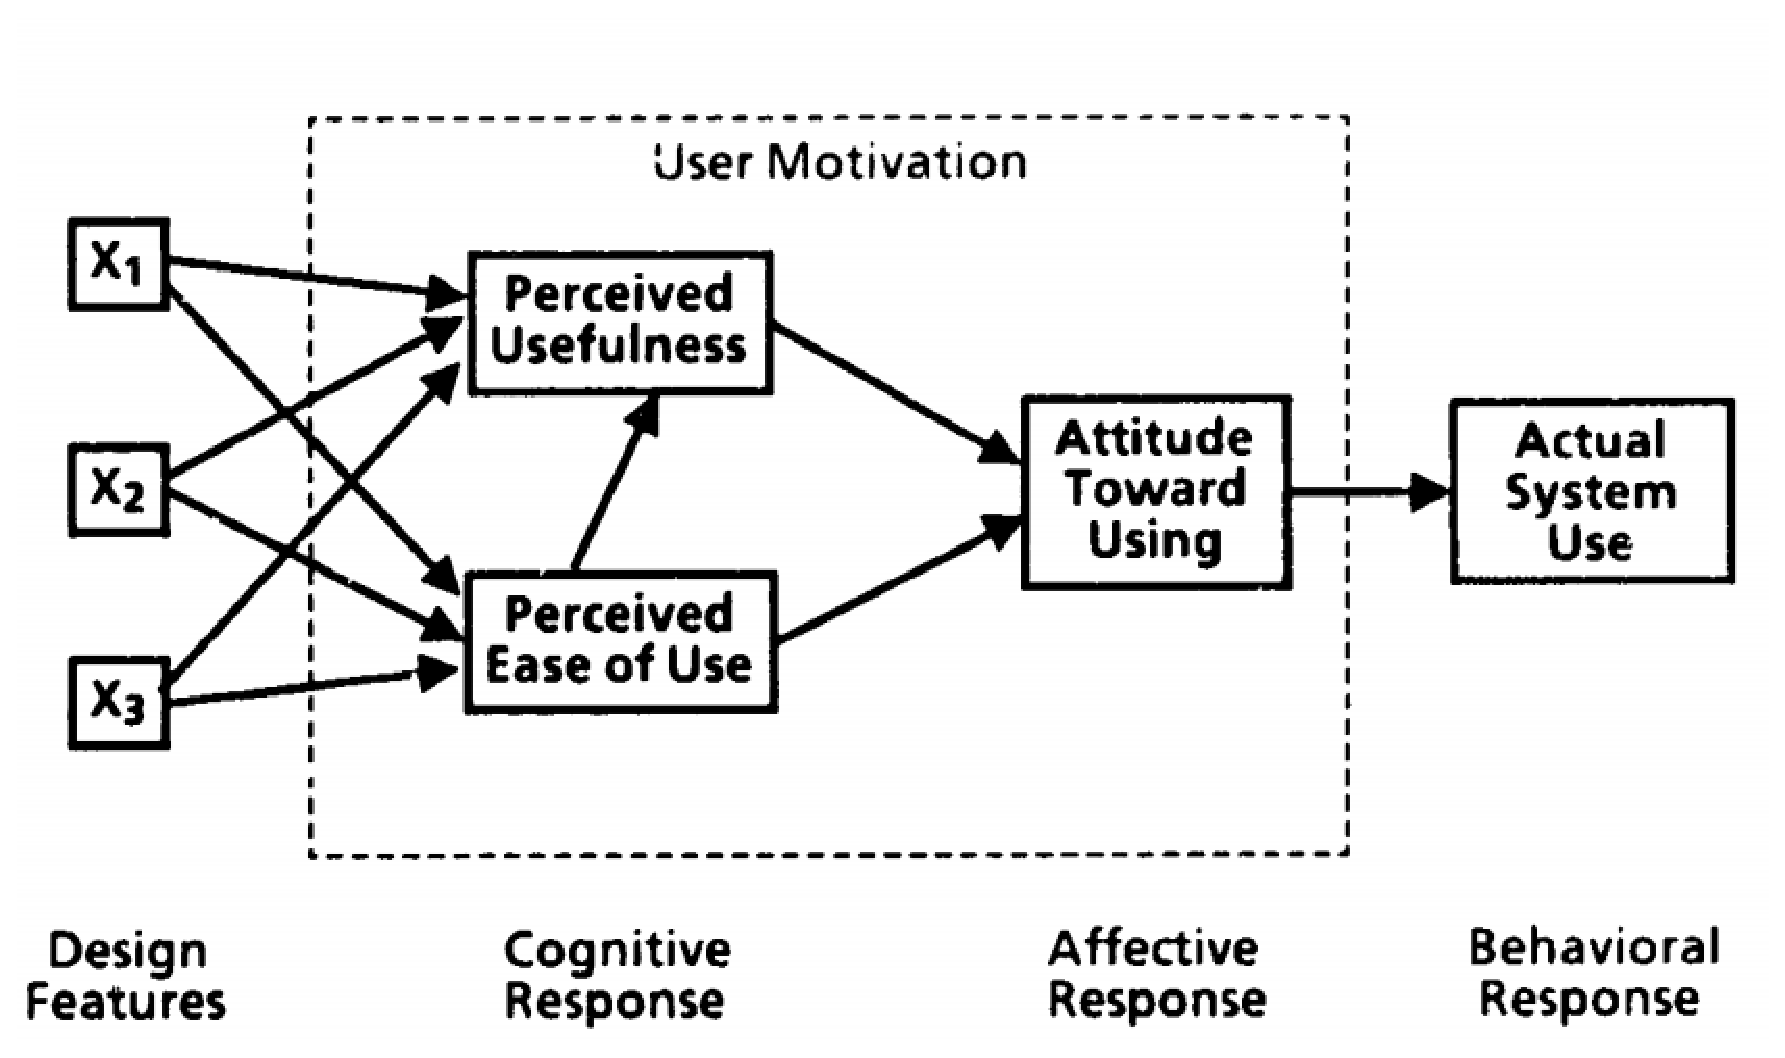
\includegraphics[width=0.6\columnwidth]{tam.eps}
		\caption{Technology Acceptance Model (TAM) \cite{davis1986technology}}
		\label{fig:tam}
\end{figure}

As Chuttur \cite{chuttur2009overview} points out in his review of TAM, there is  skepticism among some researchers regarding the rigor of the model. There exists  other assessment tools such as Game Engagement Questionnaire (GEQ) and Questionnaire for User Interaction Satisfaction (QUIS).  

Questionnaire for User Interaction Satisfaction (QUIS) \cite{harper1993improving} is a usability assessment tool developed in the HCI lab at the University Of Maryland, College Park. It is designed to assess user's subjective satisfaction regarding the human/computer interface of software systems. Currently licensing is required to access the QUIS questionnaires. 

Another usability assessment tool is the usability metrics described in Tullis and Albert 's book ``Measuring the User Experience'' \cite{tullis2010measuring}. For a usability procedure about completing transactions, Tullis and Albert suggest measuring task success, user efficiency, issues-based metrics, self-reported metrics, and live website metrics. Task success is a simple metric for a given task, does the user complete it or not? User efficiency is a measurement
of the effort required for the user to complete the task. For example, we can measure this by the amount of time spent to complete the task. Issues-based metrics involve measuring the number of times usability issues are encountered. Self-reported metrics are based on user responses to survey questions. Finally, live website metrics can be derived from analyzing the logs created by the website to understand the user experience.

\subsection{Game Metrics}

Game metrics can be as important as creativity in game design. As Nadia Oxford points out, in the game industry, player metrics collection and analysis are widely practiced to provide game designers to determine what the player audience likes and dislikes about a certain game experience \cite {Oxford2010}. 

Ducheneaut et al. provides an example of 
using game metrics to analyze player's experience in a quantitative approach \cite {ducheneaut2006alone}. They reported the relationship of playing time and leveling in the MMORGs, as shown in \autoref{fig:player-metrics}:

\begin{figure}[ht!]
	\centering
		\subfigure[Average time required to reach a level]{\label{fig:metrics1}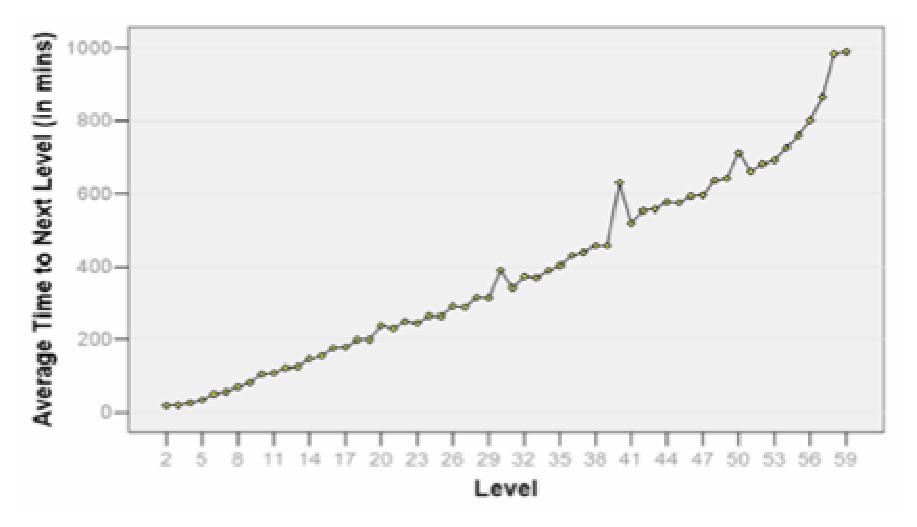
\includegraphics[height=1.7in]{metrics1.eps}}
		\subfigure[Average accumulated play time by level]{\label{fig:metrics2}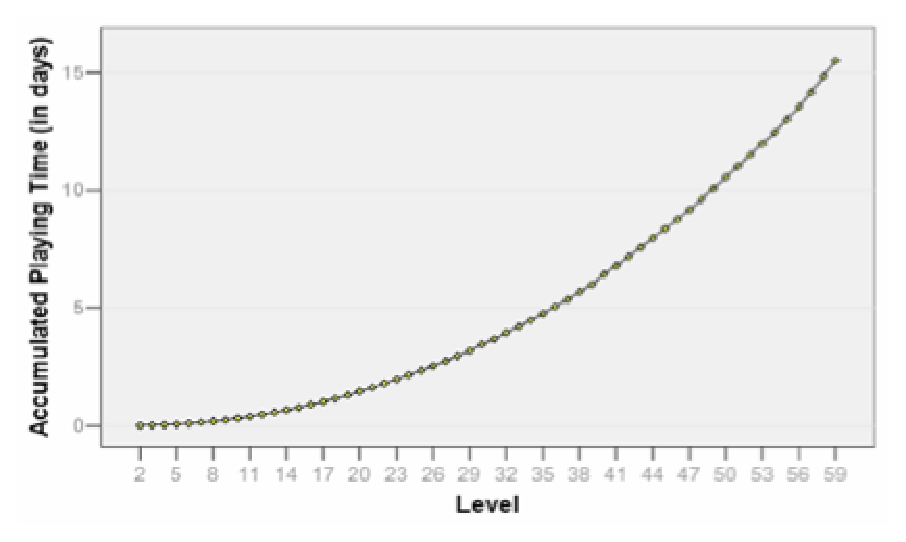
\includegraphics[height=1.7in]{metrics2.eps}}
		\caption{Player Metrics (source: Ducheneaut \cite{ducheneaut2006alone})}
		\label{fig:player-metrics}
\end{figure}

Matt Fairchild \cite {Fairchild2010} and Kontagent \cite {Kontagent2010} lists and explains some of the social games metrics as shown in \autoref{table:social-game-metrics}.

\begin{table}[ht!]
  \centering
  \begin{tabular} {|c|p{0.7\linewidth}|}
    \hline
    \tabhead{Metrics} & \tabhead{Description}\\
    \hline
	DAU & 
	Daily Active Users, is the number of active users over the course of a single day. \\
   \hline
	MAU & 
	Monthly Active Users, is the total number of users in a given month. \\
    \hline
	DAU/MAU ratio & 
	Comparing Daily Active Users to Monthly Active Users shows roughly how many days per month the average user engages with a game. \\
    \hline
	ARPU & 
	Average Revenue Per User, is measured as total revenue divided by the number of users. ARPU can be broken down by type of revenue, day, country, demographic, etc. \\
    \hline
	Churn & 
	Turnover rate (or �attrition rate�) of active players. \\
    \hline
	K Factor & 
	= (Infection Rate) * (Conversion Rate). An Infection Rate is how much a given user exposes the game to other players, such as through status updates or email invites. A conversion rate is when that ``infection'' results in a new sign up.  K factor measures the viral effect of a game. A high K Factor indicates effectiveness of bringing in new players. \\
    \hline
	Engagement &
	Measures how long users spend playing a game. How many features do they access? How many pages does the average user view? What percentage are returning visitors? \\
    \hline

  \end{tabular}
  \caption{Social Game Metrics}
  \label{table:social-game-metrics}
\end{table}

Appdata.com gathers independent application metrics from most of the social game applications. For example, the graphs in \autoref{fig:social-game-metrics} shows the DAU (Daily Active User) and MAU (Monthly Active User) metrics for the popular FarmVille \cite{farmville} social game \cite {appdata2011}:

\begin{figure}[ht!]
	\centering
		\subfigure[FarmVille DAU]{\label{fig:farmville1}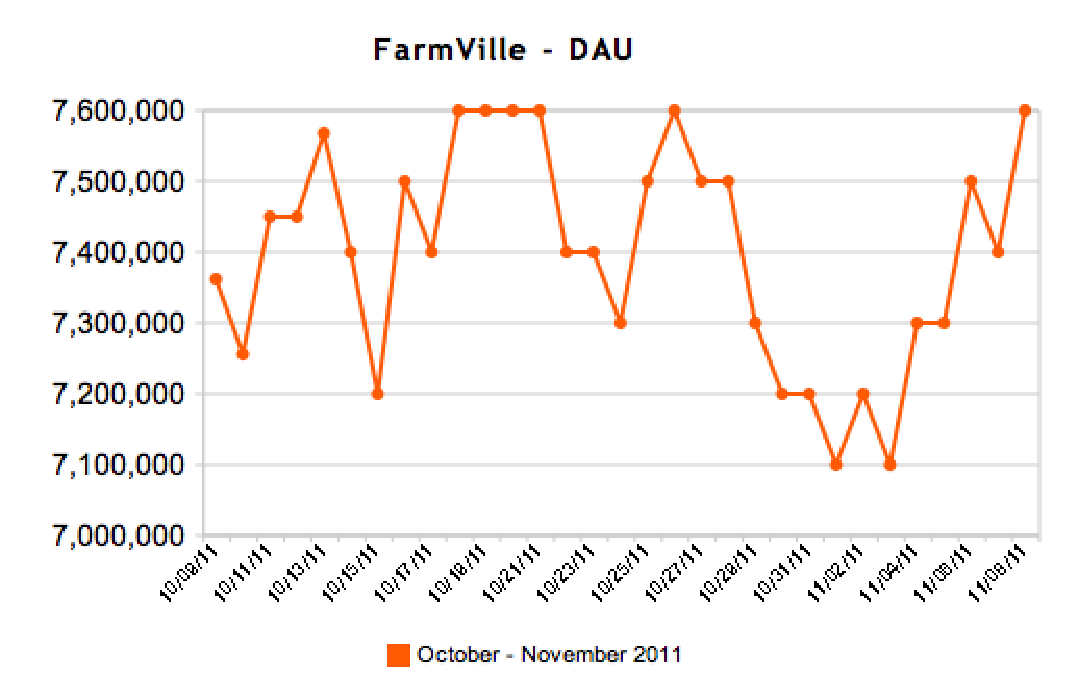
\includegraphics[height=1.85in]{FarmVille2.eps}}
		\subfigure[FarmVille MAU]{\label{fig:farmville2}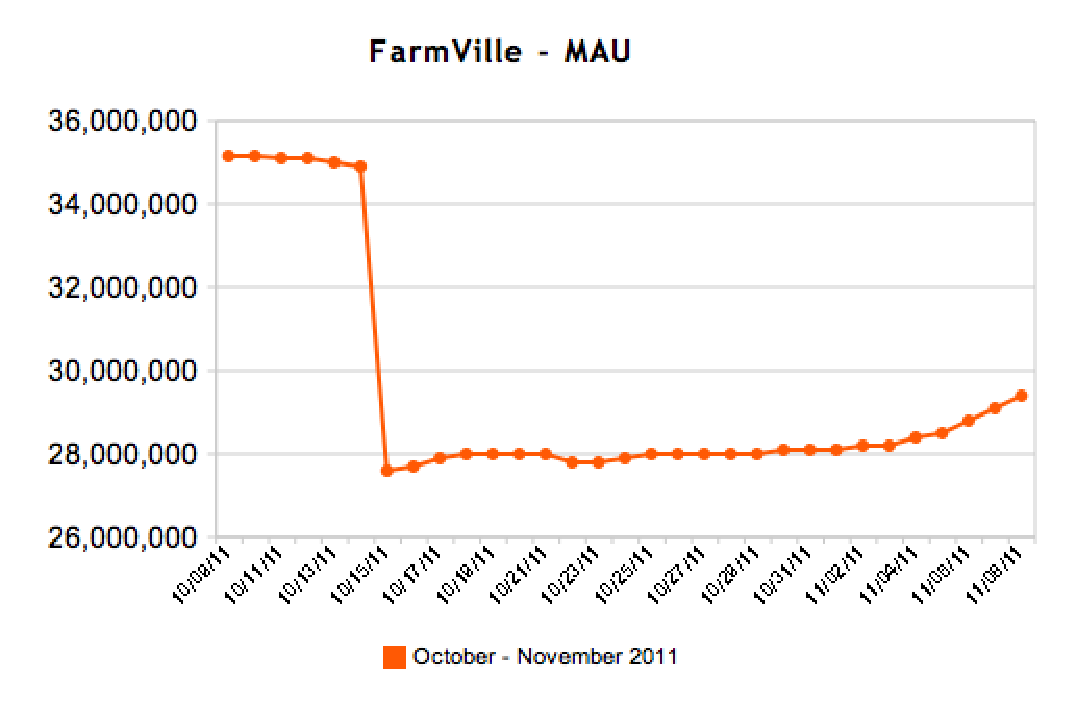
\includegraphics[height=1.85in]{FarmVille1.eps}}
		\subfigure[FarmVille DAU/MAU]{\label{fig:farmville3}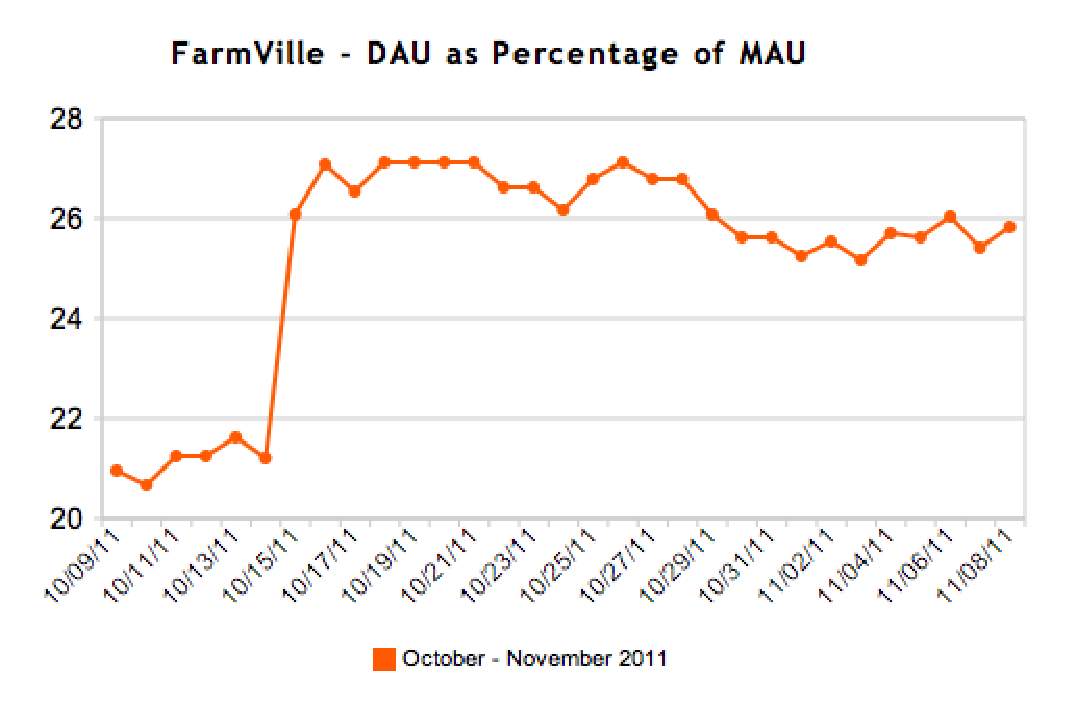
\includegraphics[height=1.85in]{FarmVille3.eps}}
		\caption{Social Game Metrics Example(source: Appdata.com \cite {appdata2011})}
		\label{fig:social-game-metrics}
\end{figure}

While the QUIS \cite{harper1993improving} is used for measuring user interaction satisfaction in a general software system, Game Engagement Questionnaire (GEQ) \cite{brockmyer2009development} developed by Brockmyer et al. is used to assess the engagement in a game. The questionnaire provides a ``psychometrically'' strong measure of levels of engagement specifically while playing video games. While the GEQ could measure the engagement level of positive game experience, the original intent of the research is to ``examine risk and protective factors for negative game impact''. \autoref{fig:geq} shows the questionnaire items.

\begin{figure}[ht!]
	\centering
		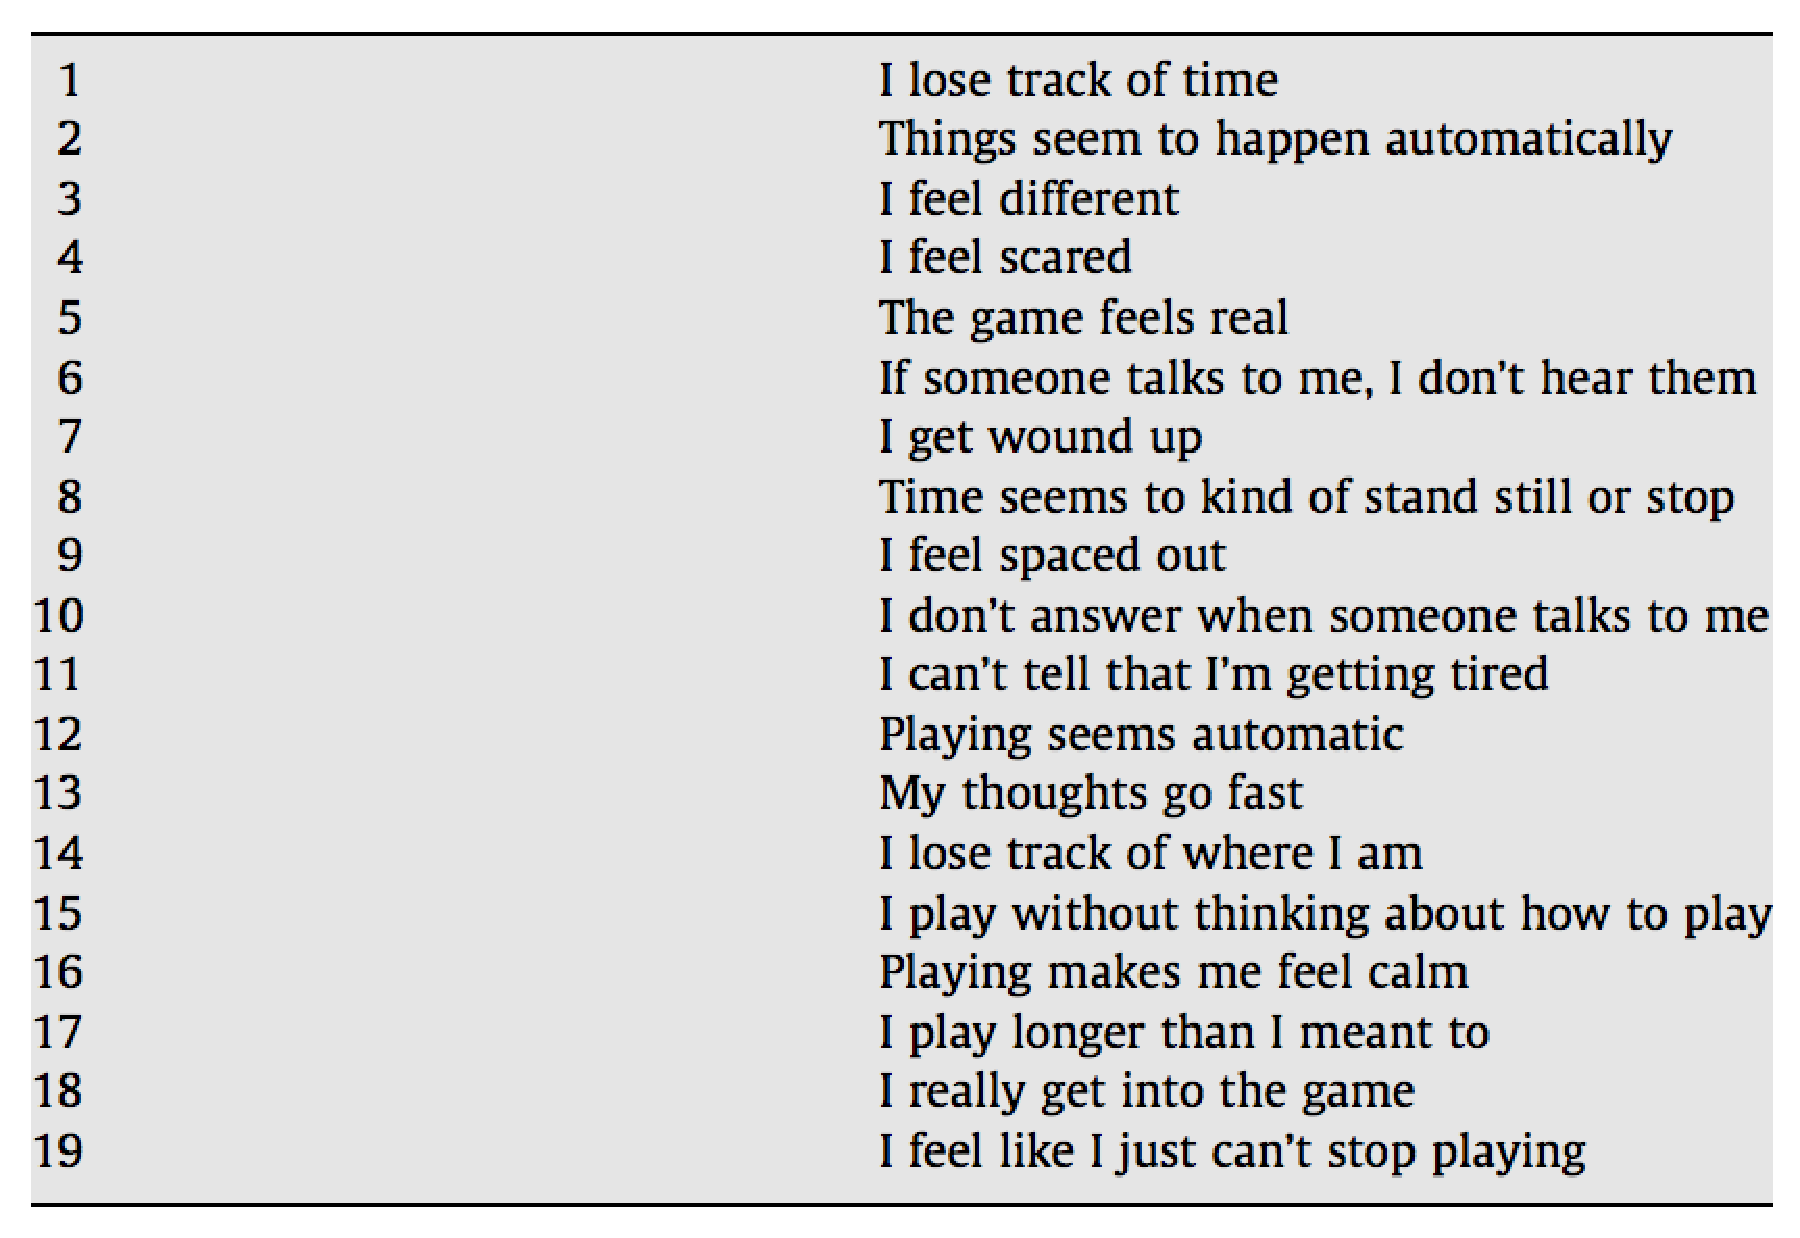
\includegraphics[width=0.7\columnwidth]{geq.eps}
		\caption{Game Engagement Questionnaire (GEQ) items \cite{brockmyer2009development}}
		\label{fig:geq}
\end{figure}

\section{Summary}
\label{sec:rel-summary}

In summary, this chapter discusses related work on serious games and gamification, game design thinking, serious games for sustainability, serious game framework and its assessment. The design of Makahiki is inspired by the current research in game design thinking in both serious games and gamification. There are some assessment methods for serious games and for general purpose such as system usability. SGSEAM is designed to provide an assessment approach for the particular needs of a serious game framework assessment.
\chapter{Makahiki Design}
\label{cha:makahiki-design}

This chapter describes the design of the Makahiki, a serious game framework for sustainability. It starts with an overview of Makahiki in Section \ref{sec:makahiki-design-overview}, followed by a  description of the Makahiki system in Section \ref{sec:makahiki-design-description}. Section \ref{sec:makahiki-design}
 describes the architecture of Makahiki, followed by the design features that make Makahiki an innovative serious game framework.

\section{Overview}
\label{sec:makahiki-design-overview}

Makahiki is an open source ``serious game framework for sustainability." It provides a framework for creating serious games for the purpose of education and behavioral change regarding energy, water, food, and waste generation and use.

The initial version of Makahiki (Version 1) was originally developed as a custom built software solution \cite{csdl2-11-01} for the Kukui Cup Energy Competition \cite{csdl2-10-08} at the University of Hawaii. The first version of Makahiki provided the following functionalities to support energy challenges at the University of Hawaii: a) A synergistic mixture of real-world and virtual world activities to raise  consciousness and literacy regarding energy issues; b) Real-time feedback on energy consumption by residence hall teams; c) Incentives in the form of prizes and raffle games. d) Social networks, both physical (residence hall teams) and virtual (Facebook).

The current version of Makahiki (Version 2) builds upon the prior version with the purpose of providing a serious game {\bf Framework} for sustainability that enables different organizations to easily create customized serious games in the context of sustainability education and behavioral change. In additional to the features from version 1, the current Makahiki framework includes the following features:

\begin{itemize}
\item The ability to tailor system functionality to support the requirements of different organizations.
\item The ability to support sustainable resource challenges such as water, food, and waste in addition to energy.
\item The ability to extend the framework with new mini-games and modules to support different requirements.
\item The use of HTML5/CSS3 ``responsive'' design techniques for support of laptop, tablet, and smart phone interfaces.
\item Real-time game analytics to help assess the impact of game mechanics during challenges.
\item Support for PaaS (Platform as a Service) facilities such as Heroku. This enables organizations to create and deploy challenges without obtaining physical hardware and its requisite IT support.
\end{itemize}

The design of Makahiki follows closely the serious game lifecycle using a framework as illustrated in \autoref{fig:serious-game-lifecycle}. In Makahiki, the system admins install or create a new default game instance by instantiating from the Makahiki framework; then the game designers configure or customize the instance according to their organization's specific needs. if needed, the game developers extend the instance by adding new game widgets. The system admins deploy the finalized instance to the infrastructure of the choice of the organization, either locally or to the cloud. Once the game instance is deployed and running, the game managers can manage the game and the players play the game. In Makahiki, the game analytics are available realtime during the game and after the game. 

The next section describes Makahiki as it is viewed by the user roles in a serious game lifecycle using the Makahiki framework.

\section{System Description}
\label{sec:makahiki-design-description}

This section describes Makahiki from the perspectives of different user roles. It first describes the installation process from the system administrator's view, followed by the descriptions of different system interfaces to players, game designers, game managers and developers.
 
\subsection{System Admin Interface}

This section describes the system admin interface of the Makahiki system from the perspective of system administrators. It includes the software installation which is part of the game instantiation, and the deployment of the instance.

The design goal Makahiki installation and deployment is to make it an easy process to support different IT infrastructure. Different organizations can choose the best installation and deployment methods that are suitable for them depending on their infrastructure and IT support capacity. 

Makahiki supports two forms of installation and deployment: local (on your own machine) and cloud-based (to the Heroku application hosting service). Organizations can install Makahiki locally if they wish to host the system themselves. This requires sufficient hardware resources and IT support to do the installation, perform backups, and monitor the system during the challenge and deal with any outages that occur.

Organizations can instead choose to host Makahiki with Heroku\cite{heroku}, a popular cloud-based Platform as Service (PAAS).  Like most cloud services, this type of installation incurs a cost depending on the service level, but has the benefit that no hardware or IT resources are required.

\autoref{table:installation} outlines the installation steps for both local and cloud environments. 

\begin{table}[ht!]
  \centering
  \begin{tabular}{|P{0.27\columnwidth}|p{0.42\columnwidth}|P{0.21\columnwidth}|}
    \hline
    \tabhead{Installation Step} &
    \tabhead{Local} &
    \tabhead{Cloud} \\
    \hline
    1. download software &
    git clone or download from website &
    git clone \\
    \hline
    2. Install tools and dependencies & 
    Python, C compiler, Pip, Virtual environment, Python Imaging Library, Memcache, PostgreSQL &
    Heroku client \\
    \hline
    3. Initialize a server instance &
    initialize\_instance &
    initialize\_instance --heroku \\
    \hline
    4. (Optional) Configure SSL & install webserver, enable SSL & addons:add ssl \\
    \hline
    5. Start up the server &
    manage.py run\_gunicorn &
    automatically started in previous step \\
    \hline
  \end{tabular}
  \caption{Installation process}
  \label{table:installation}
\end{table}

The main difference between local and cloud installation is step 2, ``Install tools and dependencies''. For a local install, all the tools and dependencies will need to be installed manually by system administrators, including the C compiler, Pip and Virtual environment, Python imaging library, memcache as the caching system, and finally the PostgreSQL database, as well as the configuration of the database. This requires adequate skills from system administrators. On the other hand, cloud installation only requires the installation of a single Heroku client. In the case of cloud installation, all  Makahiki dependencies including the PostgreSQL database are satisfied by the instance created in the Heroku cloud, thus minimizing the involvement of system administrators. 

Some organizations may want to use HTTPS / SSL to secure communication between the player browser and the website. In the local installation scenario, the system administrator can install a web server such as Apache or Nginx, then configure and enable HTTPS with SSL, and finally configure to route web requests from the web server to the Django application process. Although a fairly standard web server configuration, this local installation step requires a certain level of skill and effort. In contrast, running a Heroku client command ``heroku install addons:add ssl'' enables the SSL add-on for the application when using cloud-based hosting. For more details, please see the Makahiki installation guide \cite{makahiki-manual} chapter 2.

After the instance is created, the system admin can use the system admin interface to configure the system related settings, such as   authentication, wattdepot server connectivity, and email server. \autoref{fig:makahiki-sys-settings} shows the system admin interface.

\begin{figure}[!ht]
\begin{center}
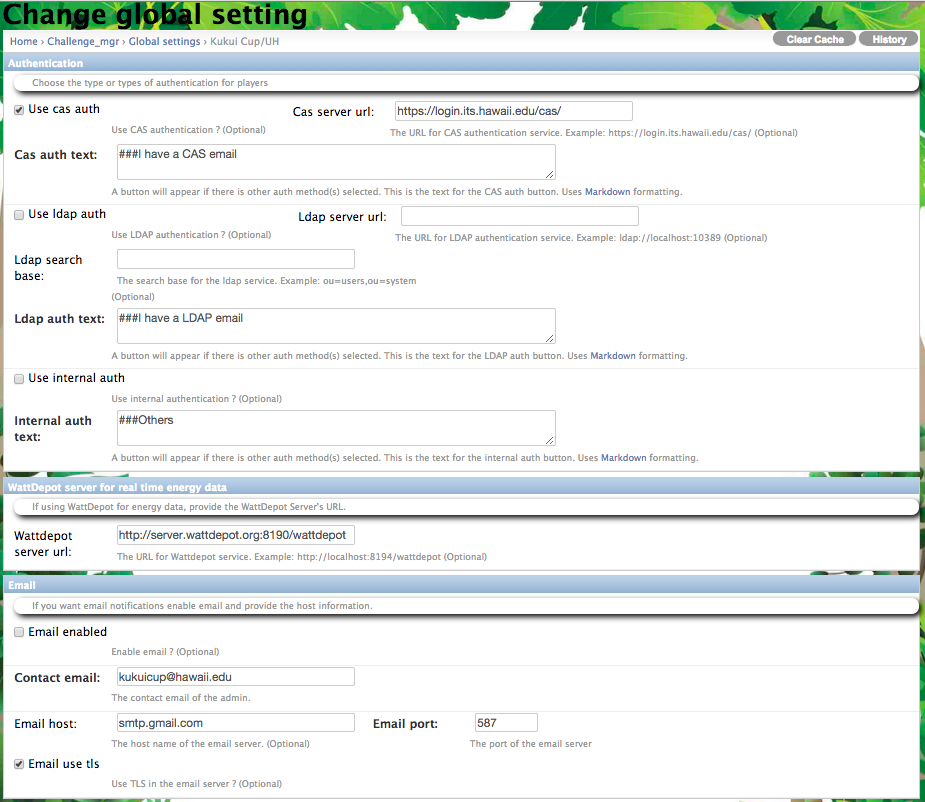
\epsfig{file=guided-tour-sys-settings, width=1\columnwidth}
\end{center}
\caption{System Admin Settings Page}
\label{fig:makahiki-sys-settings}
\end{figure}

\subsection{Game Designer Admin Interface}

Game designers use the ``Challenge Design'' admin interface to design and configure the game related settings. There are two categories of settings, one is the challenge settings, the other is the game settings. 

The challenge settings define the global configuration of the challenge such as the name and logo of the challenge, the round definition and the point system. The player settings are also defined in this section, as well as other configurable settings such as page, help, templates and the smart grid game content library. 

The game settings define the configurations for each individual games and game mechanics in Makahiki. \autoref{fig:makahiki-designer-settings} shows the challenge design interface.

\begin{figure}[!ht]
\begin{center}
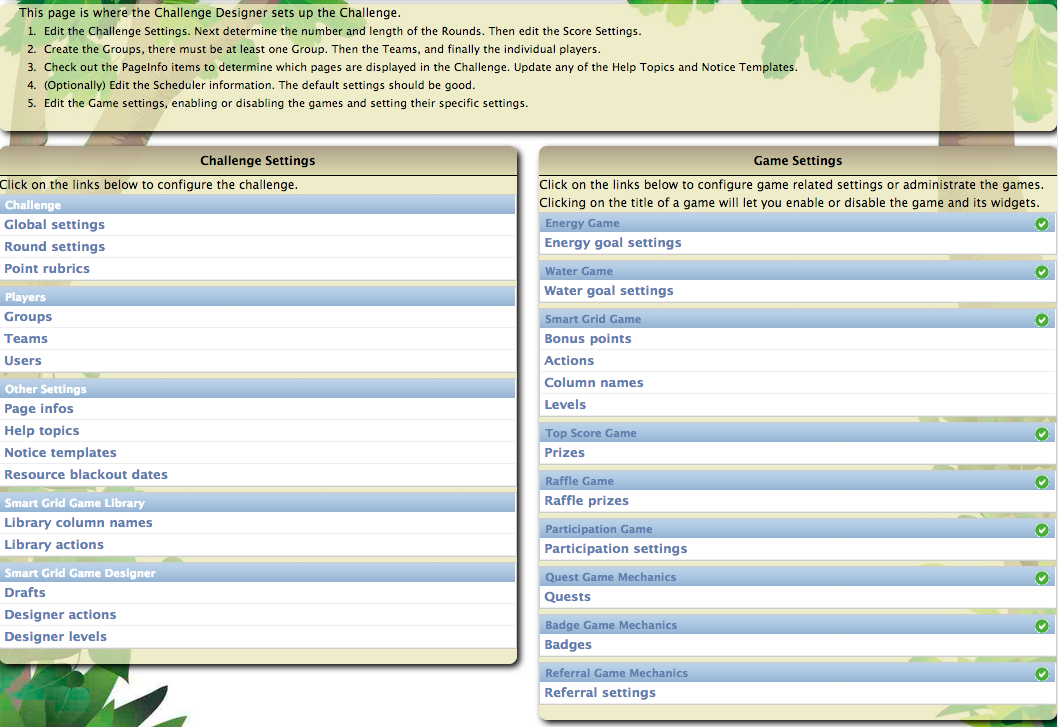
\epsfig{file=guided-tour-designer-settings, width=1\columnwidth}
\end{center}
\caption{Challenge Design Settings Page}
\label{fig:makahiki-designer-settings}
\end{figure}

\clearpage

Makahiki provides a Smart Grid Game Designer page  for game designers to design the smart grid game. It provides a WYSIWYG interface to create educational content, design the grid layout and levels. Game designers use this page to construct the Smart Grid Game, by dragging and dropping the squares (game actions) into the grid with the intended layout. The interface is shown in \autoref{fig:makahiki-designer}:

\begin{figure}[!ht]
\begin{center}
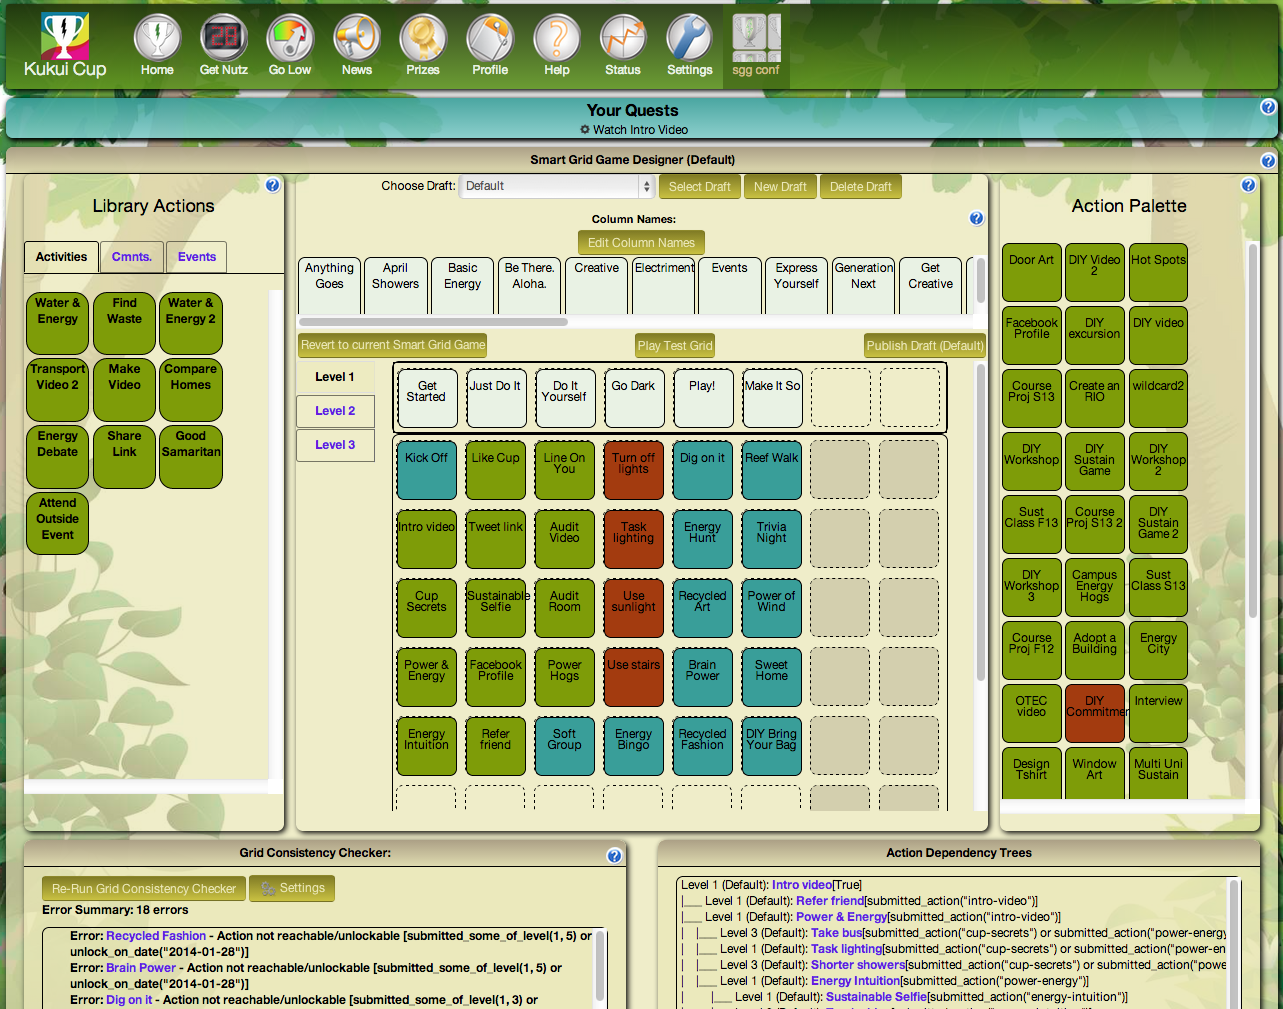
\epsfig{file=guided-tour-designer, width=1\columnwidth}
\end{center}
\caption{Smart Grid Game Designer Page}
\label{fig:makahiki-designer}
\end{figure}

\clearpage

\subsection{Player Interface}

This section describes the web interface that is viewed by the players of the Makahiki system. Because Makahiki provides the functionality for a game designer to configure and customize the game he creates, the elements and looks in the player interfaces described here are also customizable. 

\subsubsection{Landing Page}
\autoref{fig:makahiki-landing} shows a sample landing page of Makahiki system.

\begin{figure}[!ht]
\begin{center}

\epsfig{file=guided-tour-landing, width=1\columnwidth}
\end{center}
\caption{Landing page}
\label{fig:makahiki-landing}
\end{figure}

The landing page is the first page encountered by new player. So far, challenges built using Makahiki have a ``closed'' registration model; that is, the users of the system are known in advance and set up during the configuration process. Thus, the landing page has two buttons: one for users who live in a particular place and thus should have access to the system, and one for those who are just visiting and would like to learn more about the system.

Most of the content on this page is configurable, including the University logo, the slogan, the text fields and button contents, and the sponsors.

\autoref{fig:EWC-landing} shows another landing page that is customized to be used in the Kukui Cup at East West Center.

\begin{figure}[!ht]
\begin{center}
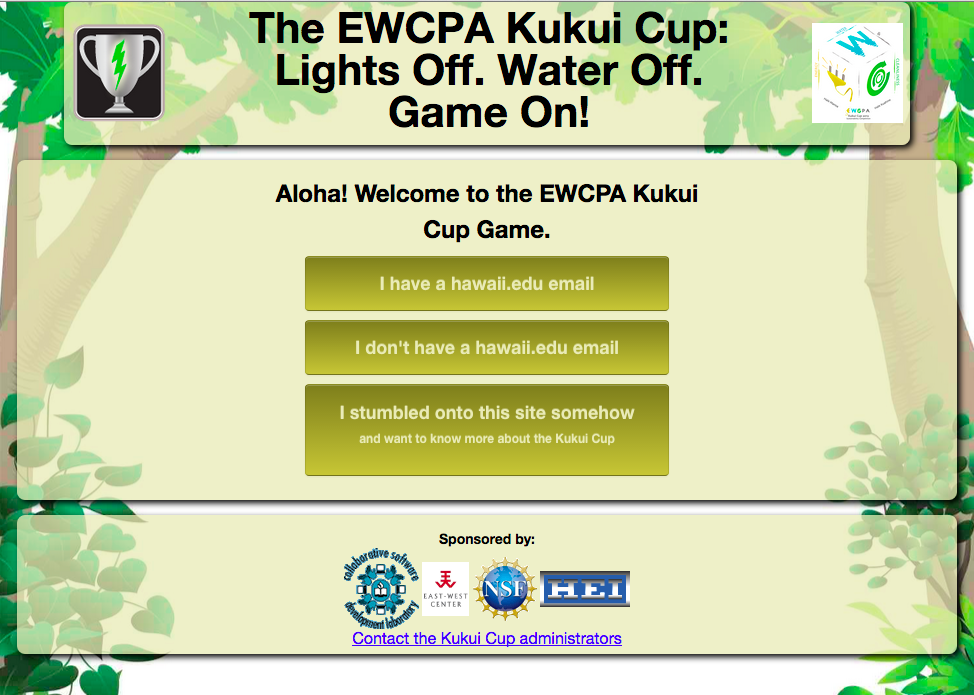
\epsfig{file=EWC-landing, width=1\columnwidth}
\end{center}
\caption{Landing page for East West Center Kukui Cup}
\label{fig:EWC-landing}
\end{figure}

\clearpage

\subsubsection{Authentication Page}

Users who click on the top button on the landing page are taken to an authentication page. Makahiki supports CAS (Central Authentication Service), LDAP, and Django internal authentication mechanisms. Different organizations can choose to configure the desired  authentication method for their game. They can use any one or combination of the above methods. \autoref{fig:makahiki-auth} shows the University of Hawaii Kukui Cup authentication screen that use the CAS authentication. \autoref{fig:EWC-auth} shows another authentication screen, the Django internal authentication, which is used in the East West Center Kukui Cup.

\begin{figure}[!ht]
\begin{center}
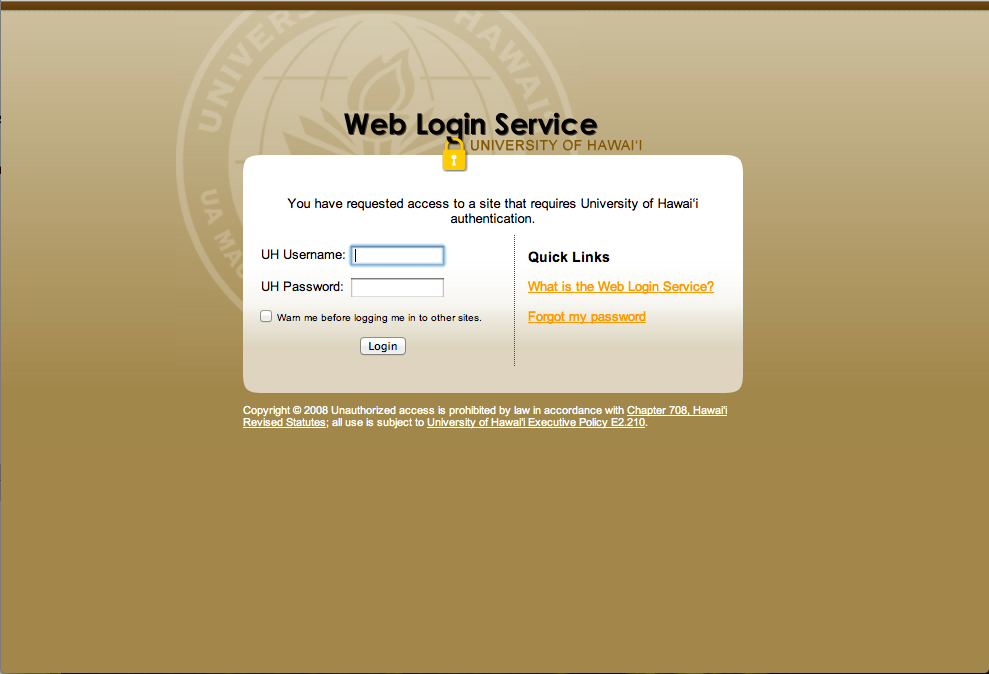
\epsfig{file=guided-tour-authentication, width=0.6\columnwidth}
\end{center}
\caption{Authentication page for University of Hawaii Kukui Cup}
\label{fig:makahiki-auth}
\end{figure}

\begin{figure}[!ht]
\begin{center}
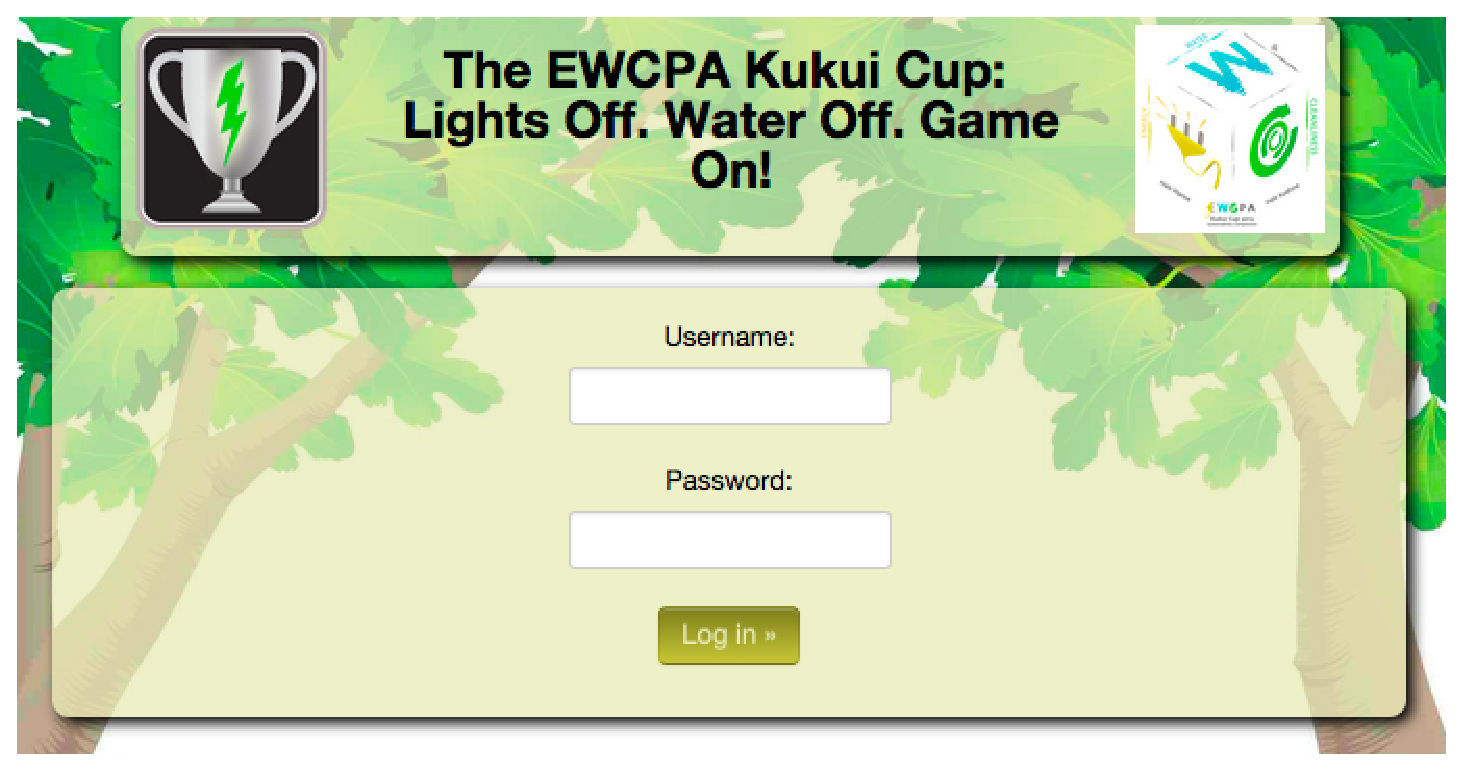
\epsfig{file=EWC-auth, width=0.6\columnwidth}
\end{center}
\caption{Authentication page for East West Center Kukui Cup}
\label{fig:EWC-auth}
\end{figure}

\clearpage

\subsubsection{Home Page}
After logging in, the players are taken to the Home page, as shown in \autoref{fig:makahiki-home}. The system sets a cookie when the player authenticates successfully, thus, after the first visit, the player will normally go directly to the home page when retrieving the challenge URL.

\begin{figure}[!ht]
\begin{center}
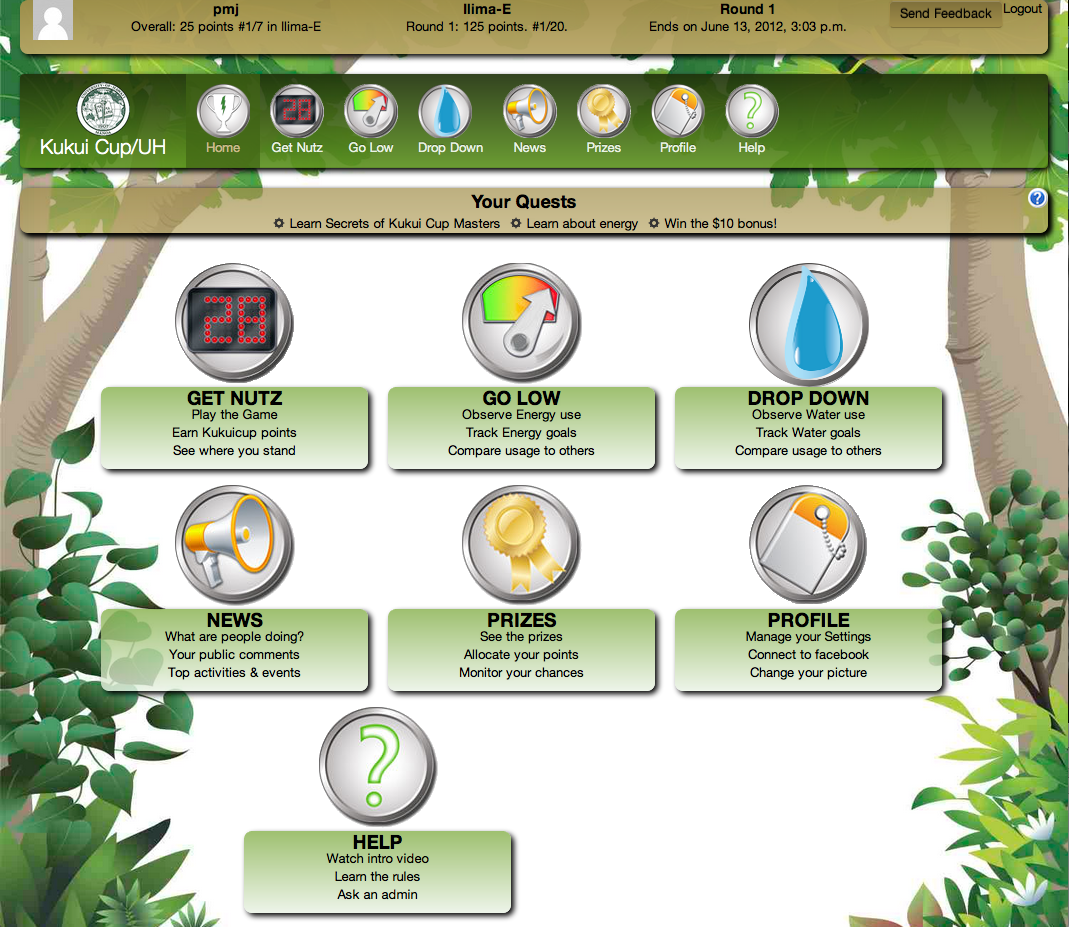
\epsfig{file=guided-tour-home, width=0.9\columnwidth}
\end{center}
\caption{Home page}
\label{fig:makahiki-home}
\end{figure}

There are three UI components in the home pages that also appear on every page. They are:

\begin{itemize}
  \item The ``Info Bar'' is a horizontal UI component at the top of every page. It provides status information about the challenge as well as a logout link. (The player will not normally need to logout unless they are accessing the site from a public computer.)
  \item The ``Nav Bar'' is a horizontal UI component below the Info Bar, which provides icons that link to all of the top-level pages in the system. The set of pages in the system is configurable.
  \item The ``Quest Bar'' is a horizontal UI component below the Nav Bar. It provides ``Quests'' (explained in more detail below).
\end{itemize}

In the center of the home page are the clickable icons and description buttons that link to the main functional pages of the game. It provides a top level glance of the functionalities of the game. The set of functional pages is configurable using the game design admin interface. \autoref{fig:HPU-home} shows another home page that is used in the Hawaii Pacific University (HPU) Kukui Cup. Note that there is no ``Drop Down'' function (for the water conservation game) in the HPU's home page.  There are two additional buttons of ``Status'' and ``Settings'' in HPU's home page which are only available to the site administrators. The background and the color theme are also different.

\begin{figure}[!ht]
\begin{center}
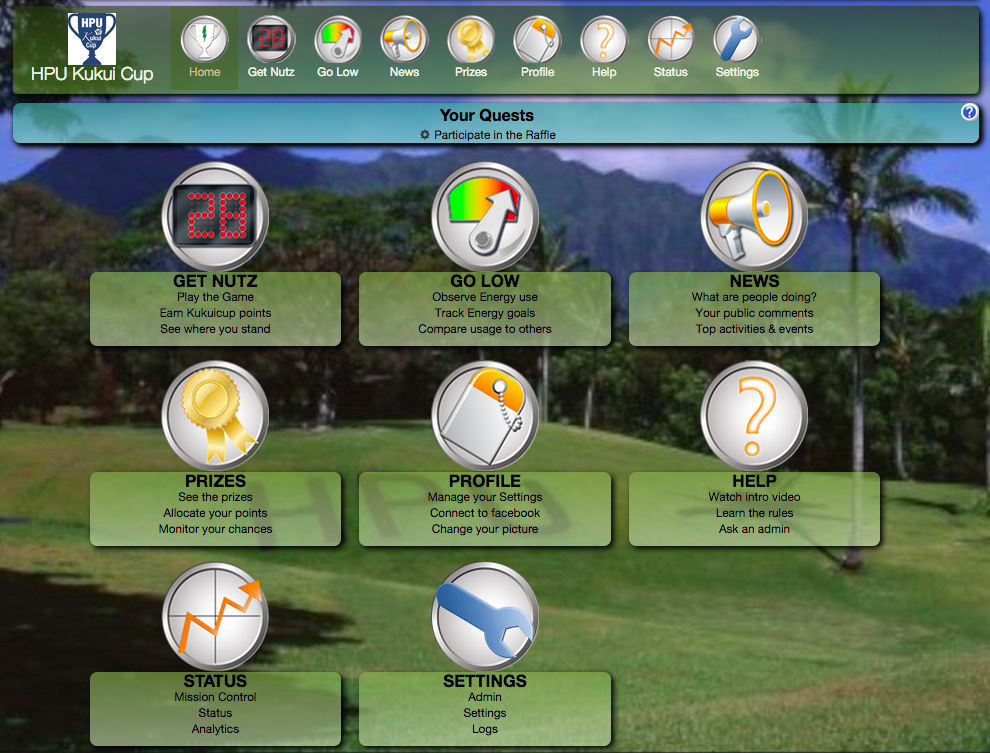
\epsfig{file=HPU-home, width=0.9\columnwidth}
\end{center}
\caption{Home page for Hawaii Pacific University Kukui Cup}
\label{fig:HPU-home}
\end{figure}

The following sections describe in detail each of these top-level functional pages.

\subsubsection{Get Nutz Page}
The ``Get Nutz'' page provides the user interface to the primary sustainability education game, also known as the ``Smart Grid Game''. Players gain points by clicking on cells in the Smart Grid UI widget, which takes them to the online or real-world educational actions such as activities, commitments and events.

\autoref{fig:makahiki-getnutz2} shows an example of the Get Nutz page (the name of this page and any other top-level page can be configured by the game designer).

\begin{figure}[!ht]
\begin{center}
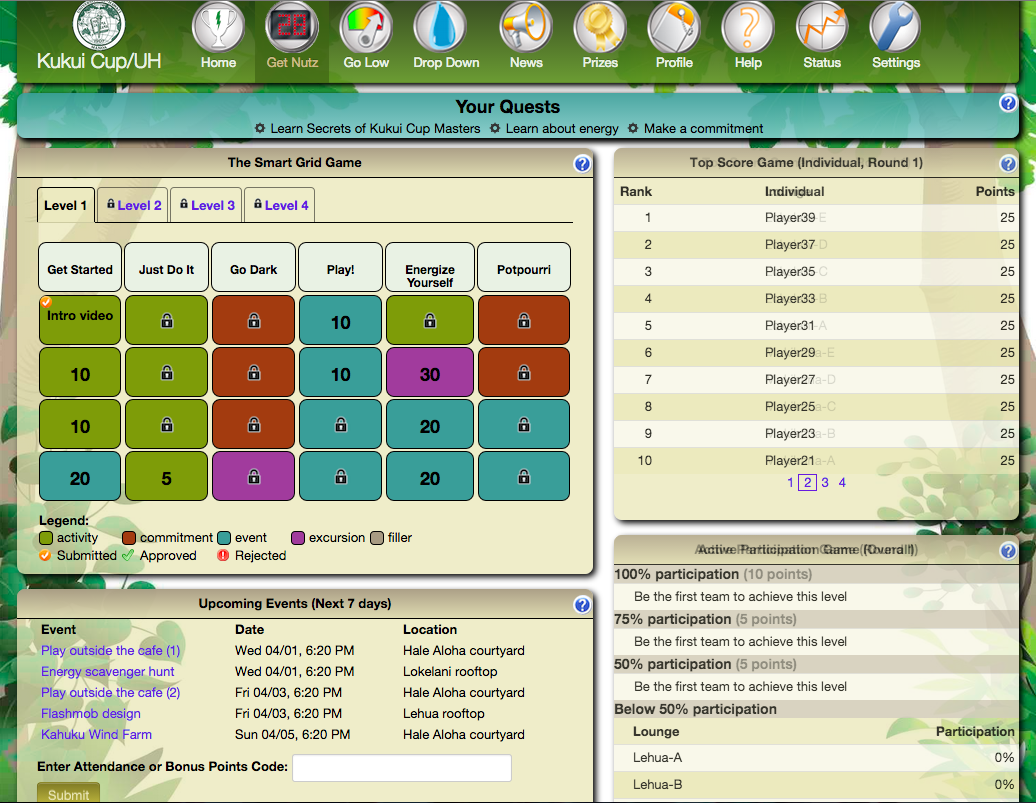
\epsfig{file=guided-tour-get-nutz2, width=0.9\columnwidth}
\end{center}
\caption{Get Nutz Page}
\label{fig:makahiki-getnutz2}
\end{figure}

The page also provides widgets about upcoming events, a scoreboard showing top scoring leaders and a widget called ``Active Participation Game.'' The set of widgets appearing on this page is configurable. The game designer can use the game design admin interface to customize what widgets to include and where the widgets appear. 

\clearpage

\autoref{fig:makahiki-getnutz} shows an another example of the Get Nutz page, which displays a different layout of the Smart Grid Game, and a different position for the ``Upcoming Events'' widget. There is no ``Active Participation Game'' in this page.

\begin{figure}[!ht]
\begin{center}
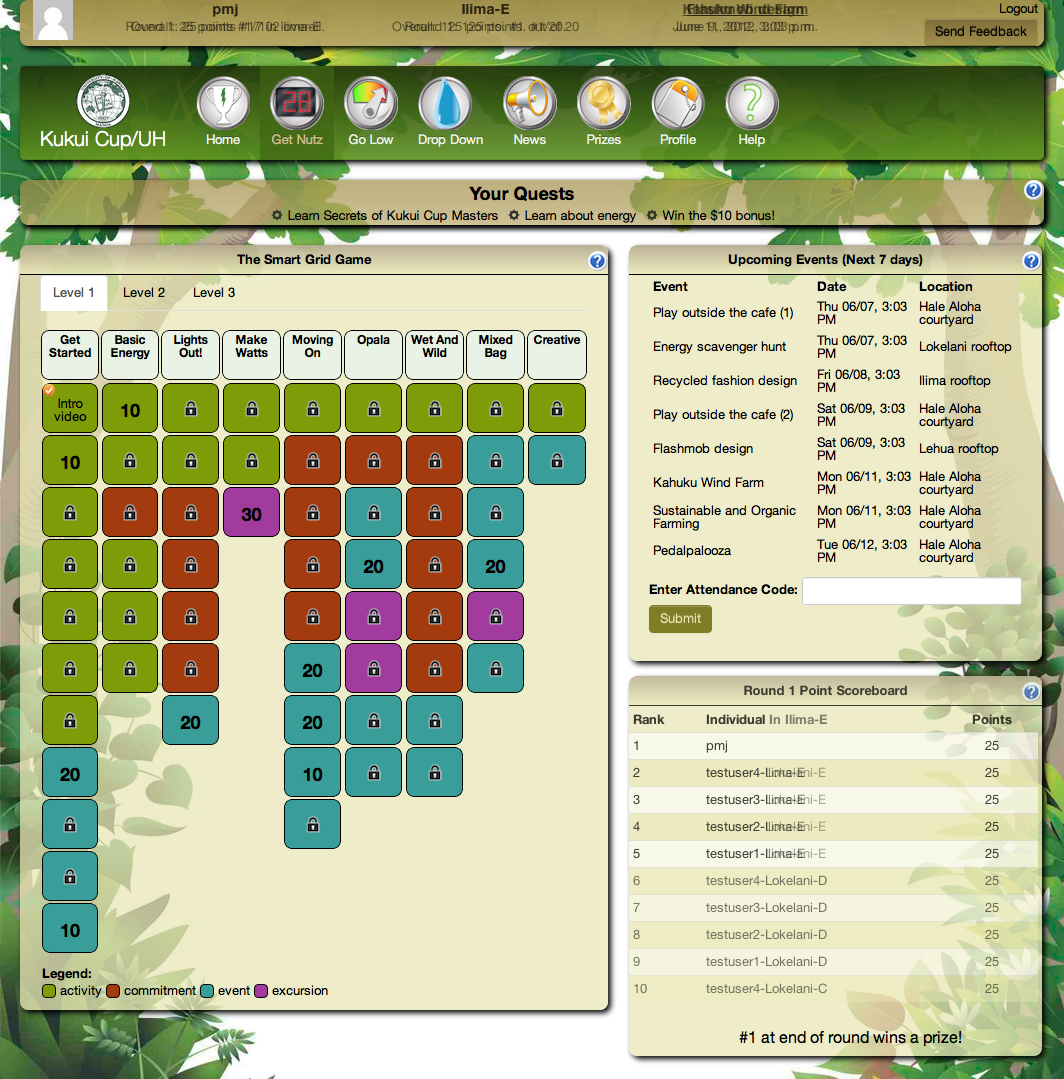
\epsfig{file=guided-tour-get-nutz, width=1\columnwidth}
\end{center}
\caption{Another Get Nutz Page}
\label{fig:makahiki-getnutz}
\end{figure}

\clearpage

Clicking on the link in the middle of the smart grid game takes the player to a page explaining that educational action.  \autoref{fig:makahiki-action} shows an example of the action page. 

\begin{figure}[!ht]
\begin{center}
\epsfig{file=guided-tour-excursion, width=1\columnwidth}
\end{center}
\caption{Action Page}
\label{fig:makahiki-action}
\end{figure}

\clearpage

\subsubsection{Go Low Page}

The ``Go Low'' page provides the user interface to two ``energy'' games, as shown in \autoref{fig:makahiki-golow}:

\begin{figure}[!ht]
\begin{center}
\epsfig{file=guided-tour-go-low, width=0.8\columnwidth}
\end{center}
\caption{Go Low Page}
\label{fig:makahiki-golow}
\end{figure}

On the left side, the ``Daily Energy Goal Game'' is designed to incentivize players to reduce their energy usage by awarding them points if they can reduce their team's energy by a certain percentage below a baseline value. The stoplight visualization tells them whether or not they are currently on track to make the reduction goal.

On the right side, the ``Current Power'' visualization helps players to see what their current power consumption is in near real-time (typically every 10-15 seconds.)

The page also enables team members to communicate via a shared chat window, and provides a scoreboard widget showing leaders in energy conservation.

\clearpage

\subsubsection{Drop Down Page}

The ``Drop Down'' page provides the user interface to the ``water'' games, as shown in \autoref{fig:makahiki-dropdown}:

\begin{figure}[!ht]
\begin{center}
\epsfig{file=guided-tour-dropdown, width=1\columnwidth}
\end{center}
\caption{Drop Down Page}
\label{fig:makahiki-dropdown}
\end{figure}

On the left side, the ``Daily Water Goal Game'' is designed to incentivize players to reduce their water usage by awarding them points if they can reduce their team's water usage by a certain percentage below a baseline value. The calendar visualization tells them whether or not they made the goal for the individual day during the current round of the competition.

On the right side, the ``Water Goal Game Scoreboard'' shows the leaders in water conservation.

\clearpage

\subsubsection{News Page}

The ``News'' page provides information about the state of the challenge and the team of which this player is a member, as shown in \autoref{fig:makahiki-news}:

\begin{figure}[!ht]
\begin{center}
\epsfig{file=guided-tour-news, width=1\columnwidth}
\end{center}
\caption{News Page}
\label{fig:makahiki-news}
\end{figure}

Widgets such as ``Lounge Members,'' ``Most Popular Excursion,'' ``My Public Commitments,'' etc. all provide a sense for the state of the competition and encourage players to participate by learning about what others members are doing.

\clearpage

\subsubsection{Prizes Page}

The ``Prizes'' page provides access to two games: the ``Top Scorer'' game and the ``Raffle'' game, as shown in \autoref{fig:makahiki-prizes}:

\begin{figure}[!ht]
\begin{center}
\epsfig{file=guided-tour-prizes, width=0.8\columnwidth}
\end{center}
\caption{Prizes Page}
\label{fig:makahiki-prizes}
\end{figure}

The Top Scorer game, illustrated by the widget on the left, shows the prizes that can be won by top scorers in the competition.

The Raffle Game provides an alternative route to win a prize. Here, players earn in-game raffle tickets based upon their point score that can be allocated to any of a collection of raffle prizes. The odds of winning are based upon the percentage of their tickets allocated to the prize, which is picked at random at the end of a round by administrators.

The Raffle Game provides an incentive for players to do activities and earn points even if they do not stand a chance of winning one of the Top Scorer prizes.

\clearpage

\subsubsection{Profile Page}

The ``Profile'' page provides access to profile information for this player, as shown in \autoref{fig:makahiki-profile}:

\begin{figure}[!ht]
\begin{center}
\epsfig{file=guided-tour-profile, width=1\columnwidth}
\end{center}
\caption{Profile Page}
\label{fig:makahiki-profile}
\end{figure}

The user can set their display name, their picture, and how they wish to be contacted for reminders. It also shows information about their badges and a complete record of how they earned all of the points in the game.

The profile page also allows them to change the theme associated with the site. A variety of themes are available. In this configuration, the default theme is ``Forest'', but users can go to the Profile page to set a different theme according to their own personal preferences. Makahiki bundles 8 different themes that can be selected from the theme dropdown menu in the Profile page. Makahiki also provides a development interface for UI developers to create more themes and include new themes into the system. 

\clearpage

\autoref{fig:makahiki-profile-theme-google} and \autoref{fig:makahiki-profile-theme-space} shows two other themes that a player can select to customize the theme for his game interface.

\begin{figure}[!ht]
\begin{center}
\epsfig{file=guided-tour-profile-theme-google, width=0.75\columnwidth}
\end{center}
\caption{Profile Page with the Google theme}
\label{fig:makahiki-profile-theme-google}
\end{figure}

\begin{figure}[!ht]
\begin{center}
\epsfig{file=guided-tour-profile-theme-space, width=0.75\columnwidth}
\end{center}
\caption{Profile Page with the Space theme}
\label{fig:makahiki-profile-theme-space}
\end{figure}

\clearpage

\subsubsection{Help Page}

The final page available to players is the Help page, which simply provides access to explanatory material about the system, as shown in \autoref{fig:makahiki-help}:

\begin{figure}[!ht]
\begin{center}
\epsfig{file=guided-tour-help, width=1\columnwidth}
\end{center}
\caption{Help Page}
\label{fig:makahiki-help}
\end{figure}

\clearpage

\subsection{Game Manager Admin Interface}

A game manager uses the ``Challenge Management'' admin interface to manage the game. He can view and search the system logs to identify errors, view the goal status for energy and water usage reduction, monitor the wall postings from the players, etc. 

In order to manage the individual games in the challenge, a game manager uses the game management section for each game. For example, in the Energy and Water game section, he can view the energy and water usage in the case of the usage data is automatically retrieved from smart meters. In the case of not using smart meters, a game manager can use this interface to manually enter the usage data. 

One important task to manage the Smart grid game is to approve the submissions from players. The game manager can use the ``Action Submissions'' link in the smart grid game management section to view the submissions and approve them, as well as generate the bonus point coupons to be handed out to players. 

\autoref{fig:makahiki-manager-settings} shows the challenge management interface.

\begin{figure}[!ht]
\begin{center}
\epsfig{file=guided-tour-manager-settings, width=1\columnwidth}
\end{center}
\caption{Challenge Management Settings Page}
\label{fig:makahiki-manager-settings}
\end{figure}

\clearpage

\subsection{Game Developer Admin Interface}

Game developers use the ``Developer'' admin interface to debug the system, add and configure new pages and games. \autoref{fig:makahiki-developer-settings} shows the developer interface.

\begin{figure}[!ht]
\begin{center}
\epsfig{file=guided-tour-developer-settings, width=1\columnwidth}
\end{center}
\caption{Developer Settings Page}
\label{fig:makahiki-developer-settings}
\end{figure}

\clearpage

\subsection{Game Analytics}

The ``Status'' page is restricted to administrators such as game designers and game managers. It provides the game analytics which displays numbers of analytics widgets about the state of an ongoing challenge and the results of the challenge. \autoref{fig:makahiki-status} shows a screenshot of part of the Status page:

\begin{figure}[!ht]
\begin{center}
\epsfig{file=guided-tour-status, width=1\columnwidth}
\end{center}
\caption{Status Page}
\label{fig:makahiki-status}
\end{figure}

The Status page is designed to help administrators monitor the progress of their challenge, detect problems with the system and/or state of play, and intercede to correct them in a timely manner.

\clearpage

\section{System Design}
\label{sec:makahiki-design}

This section describes the design of Makahiki, It first illustrates the architecture of Makahiki, followed by the descriptions of design
features that makes Makahiki an innovative serious game framework.

\subsection{Architecture}

\autoref{fig:makahiki-architecture} illustrates the overall architecture of Makahiki. The core component of Makahiki is a configurable game engine that can be customized to the needs of different organizations.  It includes two libraries of games and game mechanics. These libraries consist of a set of pre-built ``widgets.'' By selecting and configuring these game and game mechanics widgets, an organization can create a customized energy and water challenge (or serious game) in which players compete both individually and in teams, earn points by reducing their energy consumption as well as by learning about energy concepts in general, and are provided with incentives such as top score prizes and raffle prizes.  

\begin{figure}[!ht]
\begin{center}
\epsfig{file=makahiki-system-architecture, width=0.9\columnwidth}
\end{center}
\caption{Architecture of Makahiki}
\label{fig:makahiki-architecture}
\end{figure}

Makahiki interfaces with the outside environment in three different ways.

First, the top side of the architecture diagram shows that Makahiki has two primary user interfaces: one for the players of the serious game, who directly interact with the game and game mechanics widgets; the other for the administrators of the system, who configure the system and monitor the real-time game analytics.

Second, the right side of the diagram illustrates that Makahiki must obtain real-world environmental data as the challenge progresses in order to provide feedback to users about the impact of their actions. In some cases, environmental data can be input automatically into the system through a combination of ``smart'' meters and additional services (such as the WattDepot system for energy data collection, storage, and analysis). If that is not possible, then manual meters can be read by administrators on a regular (typically daily) basis and input into Makahiki using the administrator interface.

Third, the bottom side illustrates that Makahiki stores its data in a database repository (currently PostgreSQL). To reduce database access and improve performance, Makahiki provides support for caching (currently memcached).

\autoref{fig:makahiki-internal-architecture} illustrates the internal architecture of Makahiki. It provides a perspective on Maka-hiki's internal architecture in terms of three kinds of ``components'': Django-related infrastructure, Widgets, and Managers.

\begin{figure}[!ht]
\begin{center}
\epsfig{file=makahiki-internal-architecture, width=0.9\columnwidth}
\end{center}
\caption{Internal Architecture of Makahiki}
\label{fig:makahiki-internal-architecture}
\end{figure}

Managers are modules that provide Makahiki capabilities that do not involve a (player) user interface. They might provide interaction with administrators via the Django admin interface. Managers can implement game mechanic data structures (such as scores, players, and teams) or more generic web service functions (transactions, authorization, etc.)

\begin{table}[ht!]
  \centering
  \begin{tabular}{|P{0.2\columnwidth}|p{0.15\columnwidth}|p{0.55\columnwidth}|}
    \hline
    \tabhead{Manager} & \tabhead{Module Name} & \tabhead{Functionality} \\
    \hline
    Authentication Manager & auth\_mgr &
    Provides authentication services for Makahiki including administrative logins and CAS authentication \\
    \hline
    Cache Manager &  cache\_mgr &
    Manages caching data structures \\
    \hline
    Challenge Manager & challenge\_mgr &
    Maintains state information about an entire Challenge, including what widgets are enabled, the round information \\
    \hline
    Log Manager &  log\_mgr &
    Provides logging services to track the actions of logged in users \\
    \hline
    Player Manager & player\_mgr &
    Supports definition and processing of players \\
    \hline
    Resource Manager & resource\_mgr &
    Provides supports for resource management, such as updating energy or water data, checking daily goals \\
    \hline
    Score Manager &  score\_mgr &
    Manages score keeping, scoreboard calculation \\
    \hline
    Team Manager & team\_mgr &
    Support definition and management of teams \\
    \hline
  \end{tabular}
  \caption{Makahiki Internal Manager Modules}
  \label{table:managers}
\end{table}

Widgets are modules that provide Makahiki capabilities that do include a player user interface. Widgets can be roughly characterized in three ways. ``Info widgets'' provide state information about the challenge to players but little in the way of interaction. ``Mechanics widgets'' provide game elements such as Quests and Badges. The third category, ``game widgets'', refer to full-fledged interactive games.

\subsection{A Library of Configurable Games and Mechanics}

Makahiki builds in a set of configurable games and mechanics that can be turned on or off, or customized by the game designers to the needs of different organizations. The rest of this section describes these games and game mechanics and how to configure them.

\subsubsection{Selecting a Game or Game Mechanics from the Library}
A challenge designer can decide which of the built-in game and mechanics will appear in a sustainability challenge for his organization. The challenge design setting page includes a widget called ``Game Settings'', which lists the set of games available and whether or not they are currently enabled, as is shown in \autoref{fig:game-display-widget}.

\begin{figure}[!ht]
  \center
  \includegraphics[width=0.8\columnwidth]{game-display-widget.eps}
  \caption{Selecting a Game from Game Settings}
  \label{fig:game-display-widget}
\end{figure}

The small green and red icons on the right side indicate whether a game is currently enabled for the challenge. In this case, all of the games but one (Water Game) are enabled. Clicking on the title of a game will let you enable or disable the game and its widgets. After clicking on the title link in the Game Admin widget, a page similar to the \autoref{fig:game-settings} will appear:

\begin{figure}[!ht]
  \center
  \includegraphics[width=0.8\columnwidth]{game-settings.eps}
  \caption{Change a Game's Setting}
  \label{fig:game-settings}
\end{figure}

You can check or uncheck the ``enabled'' checkbox to enable or disable the game.

A game's UI is represented by a set of widgets which is visible in the game website. The widgets belonging to a game are listed under the ``Game Settings'' section, as shown in the above screen shot. If you disable the game, all the widgets belonging to this game will be hidden in the web page.

Makahiki currently allows you to create a challenge out of the following games and game mechanics:

\begin{itemize}

\item {\em Energy Game}. This game awards points to players depending upon their ability to lower their energy consumption.

\item {\em Water Game}. This game awards points to players depending upon their ability to lower their water consumption.

\item {\em Smart Grid Game}. This game is the principle interface to the educational component of Makahiki. The SGG awards points to players for successfully completing activities, commitments, excursions, and events.

\item {\em Top Score Game}. This game awards prizes to players and teams for earning the highest number of points during a round.

\item {\em Raffle Game}. This game awards prizes to players if they have allocated their raffle tickets to a particular raffle prize, and that raffle ticket was randomly selected by the system at the end of a round.

\item {\em Participation Game}. This game awards points to players if they can successfully get a certain percentage of their team members to participate in the challenge.

\item {\em Quest Game Mechanics}. This game mechanic provides a way for players to learn about features of the challenge by guiding them through Quests.

\item {\em Badge Game Mechanics}. This game mechanic provides a way for players to earn badges for playing the game in a variety of ways.

\item {\em Referral Game Mechanics}. This game mechanic provides a way for players to earn points by getting other people to participate in the challenge.

\end{itemize}

The following sections explain the design and configuration of each game and game mechanics.

\subsubsection{Energy and Water Game}

A fundamental requirement for enabling more active participation in sustainability behavior is feedback regarding their resource such as energy and water usage. The Energy and Water game in Makahiki are implemented as the Daily Resource Goal Game, which includes Daily Energy Goal Game and Daily Water Goal Game.

The Daily Energy Goal Game widget provides a way for players to see the outcome of the energy reduction behavior, and to make it a game by earning points from their behavior. By reducing their teams' daily energy consumption from a baseline by a set percentage, the players in the team will all earn a configurable amount of points. This baseline is calculated using historical data and recalculated dynamically throughout the competition. Both the baseline data and the current consumption is typically provided by API calls from Makahiki to an underlying WattDepot server. \autoref{fig:DailyEnergyGoal} illustrates this widget.

\begin{figure}[!ht]
  \center
  \includegraphics[width=0.7\columnwidth]{daily-energy-goal-game.eps}
  \caption{Daily Energy Goal Game widget}
  \label{fig:DailyEnergyGoal}
\end{figure}

As you can see, this interface uses a stoplight metaphor to show at a glance whether or not the team is making the goal. In this case, the stoplight is green, indicating they are currently below the goal.

The goal for each team is typically a percent reduction from their baseline usage. When a player goes to the ``Go Low'' page of Makahiki, they can view their team's current progress toward their daily energy goal. Near the end of the day, Makahiki checks the energy data from Wattdepot to see if a floor reached their goal. If the floor did reach their goal, each member of the floor that is participating in the game receives points. The energy goal game provides a link between the energy conservation competition and the point competition.

While the stoplight visualization provides good feedback to a team regarding their current progress toward making the current day's goal, we have found additional perspectives to also be useful.

One useful perspective to a team is a realtime power meter visualization that shows the current power usage of a team, as shown in \autoref{fig:PowerMeter}.

\begin{figure}[!ht]
  \center
  \includegraphics[width=0.5\columnwidth]{power-meter.eps}
  \caption{Power Meter widget}
  \label{fig:PowerMeter}
\end{figure}

This visualization displays the realtime power consumption which updates at a specified interval. This gives players a sense of energy consumption at the moment. For example, someone turns on a high power microwave, they might see a spike in the realtime power meter reflecting the power usage at that moment.

Another useful perspective to a team is a historical, calendar-based visualization that shows the results of the energy goal game for each day of the current round, as shown in \autoref{fig:degg-calendar}.

\begin{figure}[!ht]
  \center
  \includegraphics[width=0.7\columnwidth]{degg-calendar.eps}
  \caption{Daily Energy Goal Game Calendar widget}
  \label{fig:degg-calendar}
\end{figure}

This visualization is useful for helping teams to see if there are patterns to their ability to make their goal. The above display shows that they have been making their goal more regularly in the recent past, indicating perhaps that they have identified a useful strategy for conservation.

Yet another perspective of the energy consumption is illustrated in \autoref{fig:degg-scoreboard}. It is the Daily Energy Goal Game Scoreboard, which shows how teams are faring relative to each other. It can incentivize teams to conserve not only to earn points, but also to do better than other teams with respect to energy consumption. The scoreboard shows that the number of times that a team makes their daily energy goal and the average reduction percentage.

\begin{figure}[!ht]
  \center
  \includegraphics[width=0.6\columnwidth]{degg-scoreboard.eps}
  \caption{Daily Energy Goal Game Scoreboard}
  \label{fig:degg-scoreboard}
\end{figure}

The Daily Water Goal Game is similar to the Energy Goal game, with the only difference being the data, and whether the data is automatically or manually collected. With the installation of smart water meters and the availability of an automatic data collection system, all the visualizations discussed above will be available to the Water game. Otherwise, the water consumption data will have to be manually input daily. In this case, the hourly Water Goal Game widget and the near realtime Power Meter widget will not be available to the players, while the daily water scoreboard widget and calendar view widget will be available.

\clearpage

\subsubsection{Smart Grid Game}

Smart Grid Game (SGG) is Makahiki's approach to support ``gamified'' delivery of educational experiences. It is the primary place players go to learn about sustainability issues and earn points. Educational actions are organized into a grid of squares (hence the name ``Smart Grid'') and organized by category columns and levels. Players use its grid interface to discover ``actions'' they can perform. Successful completion of an action earns the player a variable number of points depending upon the difficulty of the action, and can potentially ``unlock'' additional actions and higher levels in the SGG. \autoref{fig:SmartGrid} shows a typical Smart Grid Game interface for players:

\begin{figure}[!ht]
  \center
  \includegraphics[width=0.8\columnwidth]{smart-grid.eps}
  \caption{Smart Grid Game widget}
  \label{fig:SmartGrid}
\end{figure}

There are three types of actions in the grid:

{\em Activities} are the most basic action available in the Smart Grid. In order to get points for an activity, a player must input a response to the system, which is reviewed and approved or disapproved by administrators. These responses can be a short textual answer or an uploaded picture. If a submission is approved, the player receives the points for their submission. Otherwise, the system notifies the player that their submission was not approved, along with a comment (written by an administrator) explaining why it was rejected. The player can change and resubmit their response and still earn the full point value for that task. 

Most activities have fixed reward points if completed. Creative activities are a special kind of activity that are worth a variable number of points, which depends on the effort made by the player and the quality of the outcome submitted. It is judged by the administrators. These activities enable players to exercise their artistic talents. 

{\em Commitments} are pledges that the player will carry out a specific action for a specific amount of time (typically 5 days). Examples include: reducing shower time, taking the stairs, and turning off the lights when leaving a room. Unlike activities, commitments are not easily verifiable, and so they are usually designed with fewer points than activities. Furthermore, a player can only enter into five commitments at any given time. After the commitment period is up, the player can declare that they completed the commitment and immediately earn the associated points. They can then enter into another commitment, including the one they just completed. 

{\em Events} are actions tied to real world meetings. To help organizers gauge interest in events, players can earn points by signing up in advance. Players that do this (and then actually attend the event) earn a signup bonus (typically 2 points). Players can also set up a reminder that is sent to their email and/or their mobile phone before the meeting takes place. At the event, a challenge administrator provides players with ``attendance codes'' printed on slips of paper that can be later entered in the system by the player to get their points. (The paper slips provide a form of verification that the player physically attended the event.) Attendance codes are generated by Makahiki and can only be used once. To discourage players from signing up and not attending, a penalty (typically 2 points) is assessed to players who do not submit an attendance code. If the player submits an attendance code for the event after receiving this penalty, the penalty is reversed. 

To make your SGG more interesting to players, and more pedagogically sophisticated, Makahiki supports the definition of ``{\em Path}'' through the educational content or actions. In most cases, when a new player sees the SGG for the first time, there should only be a few actions available to them - possibly only one. All of the rest should be locked. Makahiki provide a set of predicates that can be used to define the ``path.'' The predicates  determines if an action or level is locked or unlocked for a player, which in term depends on the outcome of another action or multiple other actions. Predicates include: completed a certain number of actions within a category, completed all actions within a category, completed  a certain action, and unlocking of an action or level after a certain date.

To incentivize players to work together during a challenge, Makahiki also supports ``{\em Social Bonus}''. The social bonus is an optional attribute of any Smart Grid Game action which awards extra points if the player has done the action with someone else. Examples of actions which commonly include a social bonus are: attending an event, recording a song related to energy, or measuring a shower water flow rate. When a player submits a response for an action that supports the social bonus, the player can provide the email address of another player who jointly completed the action. Once the other player also completes the task, the social bonus is awarded. Social bonuses are not bi-directional; if the second player does not provide the first player's email address, only the first player will get the social bonus.

Designing the Smart Grid Game is not easy; in fact, it is the most complicated task for a game designer when designing a serious game using Makahiki. Makahiki provides a tool called Smart Grid Game Designer to ease this task. The designer page is accessible only by administrators. 

\autoref{fig:game-designer} shows the basic components of the designer widget interface:

\begin{figure}[!ht]
  \center
  \includegraphics[width=0.9\columnwidth]{smartgrid-game-designer.eps}
  \caption{Smart Grid Game Designer widget}
  \label{fig:game-designer}
\end{figure}

The Designer Widget has three columns, Library Actions, Designer Grid, and Palette. 

The Library Actions Column holds a library of Activities, Commitments, and Events. The Library is a reusable set of actions for a sustainability serious game. These actions are divided into three tabs, Activities, Commitments, Events. They are generic actions without any dates or locations associated with them. You can drag these library actions into the Designer Grid. If the Action is an Event you will be asked to provide the event date and location. After the action is dragged into the grid, you can override any of the attributes of the action to be tailored to the need of a specific instance of the serious game challenge.
 
The grid that the Smart Grid Game Designer creates is called ``draft''. Designers can adjust the Designer Grid, adding or removing actions, columns and levels and players will not see the changes until they are published. Multiple drafts can be created by saving the current grid to a different name. Multiple grids allow human game designers to explore different layouts and paths through the Smart Grid Game. Once the designer is satisfied with the draft grid, he can click the ``publish draft'' button to update the live Smart Grid Game that players will see.

The Smart Grid Game Designer also includes a Grid Consistency Checker (GCC) Tool. Because of the complexity of the grid, especially the interdependency (specified by the predicates) of the grid actions, a draft grid often contains errors and inconsistencies. The GCC will be automatically run when the ``publish the draft'' button is pressed and display all the potential errors in the grid. Users should modify the draft to fix any errors found by GCC in order to successfully publish to the live smart grid game. 

\autoref{fig:smartgrid-designer-gcc-settings} shows a list of items that checked by the GCC tool. 

\begin{figure}[ht!]
  \center
  \includegraphics[width=0.7\columnwidth]{smartgrid-designer-gcc-settings.eps}
  \caption{Grid Consistency Checker Widget}
  \label{fig:smartgrid-designer-gcc-settings}
\end{figure}

\autoref{fig:smartgrid-designer-dependency} shows the action dependency tree that is inspected by the GCC tool. 

 \begin{figure}[ht!]
  \center
  \includegraphics[width=0.7\columnwidth]{smartgrid-designer-dependency.eps}
  \caption{Action Dependency Tree}
  \label{fig:smartgrid-designer-dependency}
\end{figure}

\clearpage

\subsubsection{Top Score Game}

The Top Score Game enables you to design a challenge in which prizes are awarded to individuals and teams who earn the most points during the challenge (and/or each round in a challenge). It also enables you to award prizes to the teams that conserved the most energy (or some other resource such as water) during the challenge (and/or each round in the challenge).

The Top Score Game includes both a Leaderboard widget (Figure \autoref{fig:topscore-game-scoreboard}) that shows the top players/teams in contention for each round, and a Prizes widget (Figure \autoref{fig:topscore-game-prize}) that shows the prizes for each round and the current teams/individuals in line to win them.

\begin{figure}[ht!]
	\centering
		\subfigure[TopScore Game Scoreboard]{\label{fig:topscore-game-scoreboard}\includegraphics[width=0.5\columnwidth, height=2.3in]{topscore-game-scoreboard.eps}}
		\subfigure[TopScore Game Prizes]{\label{fig:topscore-game-prize}\includegraphics[width=0.5\columnwidth, height=2.3in]{topscore-game-prize}}
		\caption{Top Score Game}
		\label{fig:topscore-game}
\end{figure}

\clearpage

Designers can configure the prizes for a particular challenge by using TopScore Game configuration on the ``Settings'' page. \autoref{fig:topscore-game-change} shows the interface to specify a prize for the challenge.

\begin{figure}[!ht]
  \center
  \includegraphics[width=1\columnwidth]{topscore-game-change.eps}
  \caption{Specifying a TopScore Game Prize}
  \label{fig:topscore-game-change}
\end{figure}

\clearpage

\subsubsection{Raffle Game}

The Raffle Game was designed to solve the problem of incentivizing players who cannot hope to be a top competitor in the Challenge. When several hundred players are competing, only a handful have a realistic chance to be the top scorers for a round. Once a player knows they cannot beat all of the other players, there can be an urge to simply give up.

The Raffle Game is designed to enable all players to have a chance to win a wide variety of prizes, where their odds of winning increase based upon the number points they have earned in the game; thus incentivize participation from all individuals, even those who are not in the running for a top prize. \autoref{fig:RaffleGame} shows an example of the Raffle Game.

\begin{figure}[!ht]
  \center
  \includegraphics[width=0.7\columnwidth]{raffle-small.eps}
  \caption{Raffle Game widget}
  \label{fig:RaffleGame}
\end{figure}

Each round of the competition has its own set of raffle prizes and any unused raffle tickets carry over to the next round. Raffle tickets are independent from a player's score, and allocating a raffle ticket does not affect their rank. The system provides random selection of the winner of each raffle item at the end of a round.

The Raffle Game works in the following way. For every 25 points (by default) that a player earns, they receive one virtual raffle ticket. Players can dynamically allocate their tickets to any raffle prizes they are interested in at any time, up to the end of the raffle. Each round of the competition has its own set of raffle prizes and any unused raffle tickets carry over to the next round. Raffle tickets are independent from a player's score; allocating a raffle ticket does not affect their rank.

As the screen image above shows, each player can see in real-time how many Raffle Game Tickets they have earned, which prizes they have allocated them to, and the resulting percentage chance they have of winning based upon the tickets allocated by others to that same prize. Of course, these odds can change on a moment-to-moment basis as players allocate and deallocate tickets.

The Raffle Game, in addition to providing an incentive for the non-top players to earn points, also creates an incentive for players to come back to the site on a regular basis to see the updated odds associated with their choices.

Designers can configure the raffle prizes for a particular challenge by using the Raffle Game Configuration link on the ``Settings'' page. \autoref{fig:raffle-game-change} shows the interface to specify a prize for the challenge.

\begin{figure}[!ht]
  \center
  \includegraphics[width=0.75\columnwidth]{raffle-game-change.eps}
  \caption{Specifying a Raffle Game Prize}
  \label{fig:raffle-game-change}
\end{figure}

The ``Winner'' of the raffle prize is randomly picked by the system at the end of the round with odds in proportion to each player's relative allocated number of raffle tickets. At the end of the page, you can also see a list of users that allocated raffle tickets for this raffle prize.

\clearpage

\subsubsection{Participation Game}

One of the design constraints of a sustainability serious game such as the Kukui Cup challenge is that, the players associated with each team in a challenge must be specified in advance of a challenge. Thus, as the challenge runs, it is possible to know exactly what percentage of each team's players are actively playing the game (in the sense that they have logged in at least once).

The Participation Game is designed to incentivize active players on a team to recruit other members of their team to login and try the game. It does this by providing extra points to all active players on a team when the percentage participation by that team reaches certain thresholds (currently 50, 75, and 100).

The current percentage participation by a player's team is shown in a scoreboard, as shown in the \autoref{fig:participation-game-scoreboard}. Players will receive an in-game notification whenever they reach a threshold participation where points are awarded.

\begin{figure}[!ht]
  \center
  \includegraphics[width=0.4\columnwidth]{participation-game-scoreboard.eps}
  \caption{Participation Game Scoreboard}
  \label{fig:participation-game-scoreboard}
\end{figure}

To configure the participation game, click on the ``Participation Settings'' link in the Participation Game Admin widget on the ``settings'' admin page. \autoref{fig:participation-game-scoreboard} shows the settings of the participation game. You can change the points to award for each participation percentage. Currently, the percentages (50, 75, and 100) are hardwired into the system.

\begin{figure}[!ht]
  \center
  \includegraphics[width=0.7\columnwidth]{participation-game-change.eps}
  \caption{Specifying a participation Game Settings}
  \label{fig:participation-game-change}
\end{figure}

\subsubsection{Quest Game Mechanics}
One fundamental challenge faced by any game is: how do players learn how to play it? This is generally known as the on-boarding problem. Makahiki provides a configurable ``Quest Engine'', that enables the definition of quests and the dependencies among them. That enables site developers to create a kind of structured, proactive user guide for the system. Instead of stumbling on a random playable feature of the game, players learn about the capabilities of the site by performing discrete sequences of actions, called ``Quests.'' 

Quests are made available to the player in a collapsible/expandable window right below the navigation bar. The set of Quests shown to a player can depend upon their game state, so that ``simple'' Quests can be presented initially and more ``complicated'' Quests presented as the player gains in expertise. Quests generally guide the player through the various workflows of the Challenge, such as completing a task, signing up for an event, or allocating a raffle ticket.

The system shows a maximum of three Quests at a time. \autoref{fig:guided-tour-quests} shows an example of an expanded quest and its content. Once the player accepts the quest, and follows the instructions to complete the quest, the notification dialog box will appear to the player indicating the accepted quest had been completed. A new potentially harder quest will appear in the quest window replacing the completed quest.

\begin{figure}[!ht]
  \center
  \includegraphics[width=0.8\columnwidth]{guided-tour-quests.eps}
  \caption{Quest Game Mechanics}
  \label{fig:guided-tour-quests}
\end{figure}

Quests are created by the administrator prior to the Challenge. Administrators have the option of specifying a set of predicates to determine when the player could be shown a Quest and when the player has completed the Quest, and it should no longer be shown.

Designers can configure the quests for a particular challenge by using Quest Game Mechanics Configuration link on the ``Settings'' page. \autoref{fig:quest-change} shows the interface to specify a quest for the challenge.

\begin{figure}[!ht]
  \center
  \includegraphics[width=0.8\columnwidth]{quest-change.eps}
  \caption{Specifying a Quest Game Mechanics}
  \label{fig:quest-change}
\end{figure}

\clearpage

\subsubsection{Badge Game Mechanics}

Makahiki provides badge game mechanics to motivate and engage players. Badge mechanics is implemented in a customizable way so that  game designers can create as many badges as they like. Each badge can be triggered by the achievement of a certain award condition, which is defined by the flexible predicate system in Makahiki. 

Badges are a common game mechanic, in which players receive recognition for various accomplishments. Makahiki allows the challenge designer to specify the set of badges available in a challenge, and to define new ones. The challenge designer has the option of making badges worth points. Finally, the designer can use the Makahiki predicate system to award a badge automatically (for example, when a player has completed a Level in the Smart Grid Game), or manually award the badge through administrator action (for example, when a player reports a significant bug in the system).

In many systems, each badge has a custom design, but in Makahiki, we decided that the overhead of providing a custom graphic for each badge outweighed the benefits. Providing a custom graphic also would create complexity with another feature of Makahiki: the ability to create ``themes'' with different colors. To be consistent with the themes in Makahiki, badges have a common look and feel consisting of a circle and a multi-character ID. Its actual colors are specified by the theme, and can thus vary from theme to theme.

\autoref{fig:badge} shows an example of the badges available in the Makahiki system:

\begin{figure}[t!]
  \center
  \includegraphics[width=0.6\columnwidth]{badge.eps}
  \caption{Badge widget}
  \label{fig:badge}
\end{figure}

Designers can configure the badges for a particular challenge by using Badge Game Mechanics Configuration link on the ``Settings'' page. \autoref{fig:badge-change} shows the interface to specify a badge for the challenge.

\begin{figure}[!ht]
  \center
  \includegraphics[width=0.8\columnwidth]{badge-change.eps}
  \caption{Specifying a Badge Game Mechanics}
  \label{fig:badge-change}
\end{figure}

\clearpage

\subsubsection{Referral Bonuses Game Mechanics}

Similar to the social bonus described in the Smart Grid Game above, the Referral Bonus is the game mechanics that help encourage participation by providing additional points to players who participate in activities with other players, and facilitate the entry of new players into an energy challenge.

Players are led through a setup process when logging into Makahiki for the first time. One of the steps in this process is the referral bonus. If a player was referred by another player in the system, they can use this step to input their email address. Once the new player earns a certain number of points in the competition, both players are awarded a referral bonus of a configurable number of points. Typically, going through the setup process gives you 25 points, so setting a point threshold of 30 points encourages the new player to at least complete one additional action in order to get the referral bonus.

When enabled, the referral bonus is implemented as a step in the first login process, as shown in \autoref{fig:referral-bonus}.

\begin{figure}[!ht]
  \center
  \includegraphics[width=0.85\columnwidth]{referral-bonus.eps}
  \caption{Referral Bonus Game Mechanics Widget}
  \label{fig:referral-bonus}
\end{figure}

If the new player was referred to the challenge by another player, they can use this step to input their email address. Once the new player earns 30 points in the competition, both players are awarded a referral bonus of (typically) 10 points. Typically, going through the setup process gives you 25 points, so a threshold of 30 points means the new player has to complete at least one additional task in order to get the referral bonus.

You can disable the referral game mechanics by clicking on the ``Referral Game Mechanics'' link. If referral game mechanics is disabled, then this window is omitted from the first login wizard and players will not be able to get points by referring other players.

The referral bonus also has a ``dynamic bonus'' capability. If enabled, then you can vary the amount of points awarded depending upon the participation level of the team associated with the new player. This incentivizes players to not just recruit new players for their own team, but to also recruit players for other teams who might not have much participation.

If the referral game mechanics is enabled, which is true by default, you will see the ``Referral settings'' link in the Game Admin widget. After clicking on the ``Referral Settings'' link, you will see the overview of the referral settings; clicking on any of the links, will bring you to a page (\autoref{fig:referral-change}) to change the settings:

\begin{figure}[!ht]
  \center
  \includegraphics[width=0.85\columnwidth]{referral-change.eps}
  \caption{Changing the Referral Bonus Game Mechanics Settings}
  \label{fig:referral-change}
\end{figure}

By default, only the ``Normal'' referral points value is used. If you check the ``Start dynamic bonus'' setting, then the ``Super'' and ``Mega'' values are enabled depending upon the team participation rate of the new player.

\subsubsection{Configuring the games in a page}
Once the games and mechanics are selected, a challenge designer can decide which games to include in a page and how the game widgets appear. He can use the ``Page info'' link in the ``Challenge Design'' admin interface to configure the game widgets and the layout of a page.  \autoref{fig:page-info-settings} shows the interface for configuring a page. 

A designer can specify the location of the widgets in the page. Currently Makahiki only supports the two-column layout in a page. The ``Location'' setting specifies whether the widget will appear in the left column or right column. The ``Priority'' setting specifies the vertical order of the widget in the column. Lower priority numbers will appear closer to the top of the column. The ``Enable'' field specifies if the widget appears or not. 

In addition to the configuration for the widgets, a designer can also configure the name of the page, whether the page should appear or not, and the location order of the page in the navigation bar.

\begin{figure}[!ht]
  \center
  \includegraphics[width=0.8\columnwidth]{page-info-settings}
  \caption{Configuring a Page}
  \label{fig:page-info-settings}
\end{figure}

\clearpage

\subsection{Configurable resource}
In Makahiki, different resources can be tracked and configured. The admin interface is built in to support the configuration of different resources. Makahiki supports three kinds of resources, which have different attributes: energy, water and waste. Some resource data can be obtained automatically from smart meters, while some resource data has to be input manually. In the case of manually data entry, the time of manual entry can be configured as well. \autoref{fig:resource} shows the Makahiki admin interface to configure the resources.

\begin{figure}[!ht]
	\centering
		\subfigure[Supported resource types]{\includegraphics[width=0.7\columnwidth]{resource.eps}}
		\subfigure[Manual resource]{\includegraphics[width=0.7\columnwidth]{goalsettings.eps}}
		\caption{Configurable resource}
		\label{fig:resource}
\end{figure}

Makahiki supports both automated and manual data collection. With respect to automated energy collection, Makahiki queries a WattDepot server once an hour to get an update on each team's consumption during the previous hour, and then updates the stoplight visualization. At midnight, Makahiki determines whether the conservation goal was achieved by the team and updates the calendar-based view with the results for that day.

However, not all challenge player communities have meters that are internet-accessible and thus allow this kind of real-time, automated update. Instead, they might have a traditional, analog meter.

The Energy Goal Game can be configured to support manual data collection. To accomplish this, the challenge designers must first tell the system the time each day at which they will read the meters manually. (To make the energy goal game workable, the challenge designers must commit to reading the energy meters for each team at approximately the same time each day so Makahiki can assume the data represents equal, 24 hour intervals. Team meters can be read at different times, but the time must be consistent for each team.)

Then, each day during the challenge, the challenge designers read the meters, then login to the system and update Makahiki with the latest readings. From this, Makahiki can determine which teams made their energy goal for the previous day.

From a user interface perspective, the basic difference is that the stoplight visualization is not available. Instead, the primary interface to the Energy Goal Game is the calendar-based visualization, which shows the results for each day.

Given support for both automated and manual energy data collection,  Makahiki can also support Water Goal Games, Food Goal Games, Waste Goal Games, or any other ``resource'' for which teams are responsible. Currently, Makahiki provides built-in support for two resource goal games: energy and water. Each of those games, when enabled, results in a page devoted to that resource in the web application. The default configuration enables support for the Water Goal Game and the Water page.

Extending Makahiki to support an additional resource goal game is straightforward, but requires developer-level capabilities.

\subsection{Real-time Analytics}

Makahiki is designed to support sustainability challenges involving hundreds or thousands of users lasting weeks or months.  In these circumstances, effective use of the technology requires the ability to understand the state of the game, such as: Who is using it? What are they doing? What is the player response to activities, commitments, excursions, and events?   Such state information is important for planning purposes, such as assessing the transportation needs for an upcoming excursion by seeing how many players signed up.   It can also be used for making in-game changes to game design, such as changing the point values associated with activities to encourage or discourage participation.  It can also help identify breakdowns in game play, such as significant numbers of unallocated raffle tickets indicating that users do not understand the nature of that game mechanic.

To address these needs and others, Makahiki includes a variety of widgets that work together to provide high level overview of game play state to the administrators of a challenge. \autoref{fig:status} shows an example of two game analytic widgets.

\begin{figure}[!ht]
  \center
  	\subfigure[User Stats]{\includegraphics[width=0.48\columnwidth, height=2.1in]{user-status}}
	\subfigure[Energy Goal Status]{\includegraphics[width=0.48\columnwidth, height=2.1in]{goal-status}}
  \caption{Game analytic widgets: User Stats and Energy Goal Status}
  \label{fig:status}
\end{figure}

The left widget, User Stats, shows trends in the total number of players, the total number of new users, and the total number of players visiting the site each day.  The right widget provides information on the ability of teams to achieve their daily energy goal each day and over time.

\autoref{table:status-widgets} lists all the analytics widgets that are currently included on the ``Status'' page. More analytics widgets can be developed using the widget development API and added to the page.

\begin{table}[ht!]
  \centering
  \begin{tabular}{|p{0.24\columnwidth}|p{0.7\columnwidth}|}
    \hline
    \tabhead{Analytics Widget} &
    \tabhead{Display Content} \\
    \hline
    Player points & Rankings of all the players' points for each round \\ \hline
    Team points & Rankings of all teams' total points for each round \\ \hline
    Team participation & Rankings of all teams' participation rate for each round \\ \hline
     Team energy & Rankings of all teams' energy usage and goal meeting status for each round \\ \hline
     Team water & Rankings of all teams' water usage and goal meeting status for each round \\ \hline
     Raffle & Number of tickets for each raffle for each round \\ \hline
     Current status & The status of the submission approval queue; number of unallocated raffle tickets \\ \hline
     Event RSVPs & Number of RSVPs for each event \\ \hline
     Popular event & Number of signups and completions for each event ordered by signups \\ \hline
     Popular activity & Number of submissions and approved for each activity ordered by submissions \\ \hline
     Popular commitment & Number of signups and completions for each commitment ordered by signups \\ \hline 
     Popular quests & Number of completed quests ordered by completions \\ \hline
     Feedback (rating) & Average ratings and total number of player feedbacks for each activity \\ \hline
     Awarded badges &  Number of players awarded for each badge \\ \hline
     Referrals & Number of referrals for the players that made a referral \\ \hline
     User stats & Graph showing the total number of players, number of new users, and number of players visiting the site for each day \\ \hline
     Energy goal status & Status of all teams' meeting energy goal each day as well as the actual usage and the difference between the usage and goal \\ \hline 
     Water goal status & Status of all teams' meeting water goal each day as well as the actual usage and the difference between the usage and goal \\ \hline 
     WattDepot status & Number of seconds taken to retrieve the Wattdepot server data for each team. \\ \hline 
  \end{tabular}
  \caption{Analytics Widgets on ``Status'' Page}
  \label{table:status-widgets}
\end{table}

\clearpage

\subsection{Responsive mobile support}
We believe that mobile support is essential for this kind of sustainability challenge, especially for the new generation players. Makahiki implemented  responsive web design technology to support multiple devices to enhance the player experience. \autoref{fig:responsive} shows the responsive interface in Makahiki that supports both desktop view and mobile view with the same code base.

\begin{figure}[!ht]
  \center
  \includegraphics[width=1\columnwidth]{responsive.eps}
  \caption{Responsive design supports both desktop and mobile}
  \label{fig:responsive}
\end{figure}

\clearpage

\subsection{Cloud deployment support}
Another feature in Makahiki is the ability to deploy to a Cloud platform. Cloud computing has the advantage of simplifying IT administration by eliminating the need to acquire the hardware, install software etc, thus lowering the cost of software deployment. \autoref{fig:heroku} shows a screen shot of the Dashboard showing the 2012 East West Center Kukui Cup challenge deployed in Heroku, a cloud platform provider. The monthly cost for the IT infrastructure in this instance is quite affordable. 

\begin{figure}[!ht]
  \center
  \includegraphics[width=0.9\columnwidth]{heroku.eps}
  \caption{Heroku cloud deployment}
  \label{fig:heroku}
\end{figure}

\autoref{section:cloud-hosting} describes in details our experiences with several real world Makahiki instances that are deployed to the Heroku cloud infrastructure. In general, for a small organization, a monthly cost of \$10 for hosting a Makahiki game instance is sufficient, such as in the East West Center case. For a large organization with about 1000 eligible players, the monthly hosting cost will be around \$100. See \autoref{section:cloud-hosting} for more discussions on the cost of cloud hosting.

As discussed in \autoref{section:cloud-hosting}, besides the cost benefit, cloud deployment has the the advantage of dynamically adjusting the computing resource for the application in both scaling up and scaling down scenarios. 

\subsection{Customization and Extension Development Support}
Makahiki, as a framework, provides facilities to help developers to create customizations and extensions to fit different requirements from the organization. The following section describes the two customizations that can be implemented by developers through minimal programming.

\subsubsection{Theme Development}
A ``theme'' in Makahiki consists of a specification of the background image (or color), as well as the background and font colors for various structural elements of the system. Players have the ability to select themes from the Profile page, making it unnecessary to develop a ``perfect'' theme for your challenge. \autoref{fig:theme-change} shows the widget that a player can use to change the theme they like the best for their personal website feel. 

\begin{figure}[!ht]
  \center
  \includegraphics[width=0.6\columnwidth]{theme-change}
  \caption{Change the Website Theme}
  \label{fig:theme-change}
\end{figure}

Makahiki provides a set of pre-built themes for players to choose from. \autoref{fig:theme-installed} lists all the installed themes in Makahiki. These installed themes will show up in the ``Theme'' drop-down that can be selected by a player as shown in \autoref{fig:theme-change}.

\begin{figure}[!ht]
\begin{lstlisting}
##########################################################
# INSTALLED Themes. Please keep them in alphabetical order
##########################################################
INSTALLED_THEMES = (
    'theme-bubbles',
    'theme-bumblebee',
    'theme-forest',
    'theme-google',
    'theme-hpu',
    'theme-revolusun',
    'theme-sonora',
    'theme-space',
    'theme-wave',
)
\end{lstlisting}
\caption{Makahiki Pre-Built Themes Defined in settings.py}
\label{fig:theme-installed}
\end{figure}

Makahiki, as a framework, allows developers to create additional themes. Makahiki's themes are implemented using LESS, which is the  enhanced version of CSS that supports variables and other capabilities not available in standard CSS. There is no need to know about LESS in order to create Makahiki themes. Most developers should be able to create themes simply by copying and editing a pre-existing theme file and changing some of the LESS variables in the new file. All the theme files are located in the ``makahiki/static/less'' directory.  Most of the times, a theme developer only needs to pick the color for the theme and specify which color he want for a specific UI elements in the LESS file. \autoref{fig:theme-google-less} shows a snippet of the theme-google.less file.

\begin{figure}[!ht]
\begin{lstlisting}
// Google color palette
@google-white:          #FFFFFF;
@google-offwhite:       #E9EEF5;
@google-lightblue:      #8DAAEB;
@google-gold:           #E8AC13;
@google-lightlightblue: #B8CAE0;
@google-darkblue:       #1249E0;
@google-red:            #D41C34;

// Page Background
@use-bkg-image: false;
//@page-bkg-image: "../images/forest-theme-background.jpg";

@page-bkg-color-start: @google-white;
@page-bkg-color-end: @google-white;
@page-font-color: @black;
@page-link-color: @google-darkblue;

// Widgets
@widget-title-bkg-color-start: @google-lightblue;
@widget-title-bkg-color-end: @google-lightblue;
@widget-title-font-color: @black;
@widget-title-transparency: 0%;
@widget-body-bkg-color: @google-white;
@widget-body-font-color: @black;
@widget-body-transparency: 0%;

// Smart grid game
@sgg-header-bkg-color: @google-offwhite;
@sgg-header-font-color: @black;
@sgg-entry-font-color: @black;
@sgg-activity-cell-bkg-color: @google-lightblue;
@sgg-commitment-cell-bkg-color: @google-red;
@sgg-event-cell-bkg-color: @google-gold;
@sgg-excursion-cell-bkg-color: @google-darkblue;
@sgg-filler-cell-bkg-color: lighten(@black, 30%);

\end{lstlisting}
\caption{Google Theme defined in theme-google.less}
\label{fig:theme-google-less}
\end{figure}

Once the theme file is created, it should be included in the ``INSTALLED\_THEMES'' section in the settings.py file as shown in the previous \autoref{fig:theme-installed}. To see the results of the new theme, Makahiki provides a special page called ``theme-display''. The developer can use the browser to go to this page to test all of the theme-able elements in a single page. \autoref{fig:theme-google-test} illustrates the result of the new theme.

\begin{figure}[!ht]
  \center
  \includegraphics[width=0.99\columnwidth]{theme-google}
  \caption{The Result of theme-google.less}
  \label{fig:theme-google-test}
\end{figure}

\subsubsection{New Game Widget Development Support}

As discussed previously, Makahiki includes a set of pre-built game and game mechanics widgets for game designers to select and configure for their serious game challenges. In some cases, game designers may wish to implement additional games or mechanics and integrate them into the Makahiki system. It is achievable through the game widget development support of the Makahiki framework. In order to develop new games, programming knowledge of Python and Django is required. This is unlike the theme development where there is no need to know LESS or any programming. 

Developing a new widget for Makahiki includes the following four steps:

The first step is to create the new widget package structure. Makahiki provides a command line tool called ``startwidget'' integrated into the standard Django manage.py utility. It is the easiest way to create the basic file structure for a new widget. \autoref{fig:startwidget} illustrates the command to create a hello\_world widget and the base files and directory structure that are created by the tool. 

\begin{figure}[!ht]
\begin{lstlisting}
% manage.py startwidget hello_world
\end{lstlisting}
\begin{lstlisting}
hello_world/
            __init__.py
            views.py
            tests.py
            templates/
                      index.html
\end{lstlisting}
\caption{Makahiki Tool for Creating a New Widget Structure}
\label{fig:startwidget}
\end{figure}

The command creates a directory named after the new widget in the directory ``apps/widgets'', and four files underneath:
\begin{itemize}
\item {\em \_\_init\_\_.py}: this file indicates that the directory is a Python package.
\item {\em views.py}: this file implements the widget logic and provide data to the UI.
\item {\em index.html}: this file defines the UI that is displayed to players.
\item {\em tests.py}: this file provides the skeleton of the unit testing for the new widget.
\end{itemize}

These files are the starting points for building a new widget.

The second step is to implement the logic of the widget and provide the data for display. It is done in the views.py by calling the Application Programming Interfaces (APIs) provided by Makahiki. 

The Makahiki API provides a generic mechanism for supplying data to display in the widget UI.  When the player loads a page, the Makahiki module ``{\bf apps.pages.views.index}'' is called. This module determines the name of the page dynamically and creates a Python dictionary, called ``{\bf view-objects}''.  From the page configuration, it determines which widgets are enabled for the given page. It then loops over each widget and calls their ``{\bf apps.widgets.widget\_name.views.supply}'' function. So the entry point for the widget is the supply function in its views.py file. 

The startwidget command provides the empty supply function in the views.py it created, as shown in \autoref{fig:views}. 
\begin{figure}[!ht]
\begin{lstlisting}
"""Provides the view of the widget."""
def supply(request, page_name):
    """ supply view_objects for widget rendering."""
    _ = request
    _ = page_name
    return {}
\end{lstlisting}
\caption{Supply function template provided in the base views.py}
\label{fig:views}
\end{figure}

A developer needs to fill in the supply function to provide the data. Makahiki also includes a library of manager modules that provides APIs to interact with the system. \autoref{table:managers} lists all the manager modules and their functionality. 

For illustration purpose, the hello\_world widget will display three kinds of data obtained from the Makahiki system. One is the name of the player, which is stored in the name attribute of profile object. The second is the name of the team the player belongs to. It is stored in the team attribute of the profile object. The third data is the current point score of the player. It can be retrieved by calling the function ``player\_points'' in the ``score\_mgr'' module. \autoref{fig:views-example} shows the complete example of views.py for hello\_world widget.

\begin{figure}[!ht]
\begin{lstlisting}
"""Provide the view for the Hello_World widget."""
from apps.managers.score_mgr import score_mgr
def supply(request, page_name):
    """Supply view_objects contents, which are the player name, team and points."""
    _ = page_name
    profile = request.user.profile
    name = profile.name
    team = profile.team
    points = score_mgr.player_points(profile)
    return {
        "name": name,
        "team": team,
        "points": points,
    }
\end{lstlisting}
\caption{Example of a completed views.py}
\label{fig:views-example}
\end{figure}

The third step in creating a new widget is to declare the UI component. It is done in index.html under the templates directory.
\autoref{fig:index-base} shows the base index.html created by the ``startwidget'' command.

\begin{figure}[!ht]
\begin{lstlisting}
<div class="content-box">
    <div class="content-box-title">
        Widget name
    </div>
    <div class="content-box-contents">
        Widget content
    </div>
</div>
\end{lstlisting}
\caption{Generated base index.html}
\label{fig:index-base}
\end{figure}

Makahiki provides many different styles and CSS classes. Normally, widgets are contained in a content-box. A context-box is a rounded, shaded box with two parts, content-box-title, and content-box-contents. A developer can replace the ``Widget name'' in the title box and the ``Widget content'' in the content box to display the data provided from views.py. A complete example of the index.html file of the hello\_world widget is shown in \autoref{fig:index-example}. The data provided from the views.py are referenced by the convention of ``{\bf view\_objects.widget\_name.variable}''.

\begin{figure}[!ht]
\begin{lstlisting}
<div class="content-box">
    <div class="content-box-title">
        Hello World Widget
    </div>
    <div class="content-box-contents">
        Welcome <b>{{ view_objects.hello_world.name }}</b>, <br/>
          you're in team <b>{{ view_objects.hello_world.team }}</b> <br/>
          you have <b>{{ view_objects.hello_world.points}}</b> points.
    </div>
</div>
\end{lstlisting}
\caption{Example of a completed index.html}
\label{fig:index-example}
\end{figure}

Finally, the fourth step for developing a new widget is to add the widget to a page. In order for a new widget to be available to the system, you need to edit the Makahiki ``settings.py'' file and add the widget name to the INSTALLED\_WIDGET\_APPS variable. \autoref{fig:installed-widget} shows a portion of the settings.py file after adding the new hello\_world widget. 
\begin{figure}[!ht]
\begin{lstlisting}
################################
# INSTALLED Widgets
################################
INSTALLED_WIDGET_APPS = (
  'action_feedback',
  'ask_admin',
  'badge_scoreboard',
  'badges',
  'bonus_points',
  'hello_world',
  'home',
  ....
  )
\end{lstlisting}
\caption{Adding the new widget to settings.py}
\label{fig:installed-widget}
\end{figure}

This last step makes the newly developed widget available to the Makahiki system. Once it is available to the system, a game designer will be able to add the widget to an existing page using the admin interface.

The ``Page Settings'' link in the admin interface is used to configure the widgets in a page. \autoref{fig:page-settings} shows the hello\_world widget being added to the existing Profile page.

\begin{figure}[!ht]
  \center
  \includegraphics[width=0.99\columnwidth]{page-settings}
  \caption{The Hello World widget added to the left column}
  \label{fig:page-settings}
\end{figure}

The hello\_world widget is added to the left side location with the priority set to ``1'', which indicates that the new widget will be displayed first and before the ``My Info'' widget (priority 2) on the left side column on the page.  The widget will also need to be enabled by checking the ``enabled'' checkbox. \autoref{fig:hello-world-widget} shows the final result of the hello\_widget displayed in the Profile page.
\begin{figure}[!ht]
  \center
  \includegraphics[width=0.99\columnwidth]{hello-world-widget}
  \caption{The Hello World widget displayed in the Profile page}
  \label{fig:hello-world-widget}
\end{figure}

\section{Summary}
Makahiki is designed to provide an easy to use framework for different organizations to create custom sustainability related serious games. 

Makahiki provides a libraries of games and game mechanics for organizations to choose and customize from. \autoref{table:makahiki-games} lists the Makahiki built-in games and game mechanics.

\begin{table}[ht!]
  \centering
  \begin{tabular} {|P{0.2\linewidth}|P{0.6\linewidth}|P{0.1\linewidth}|}
    \hline
    \tabhead{Name} &
    \tabhead{Description} &
    \tabhead{Type} \\
    \hline
    Energy Game & awards points to players depending upon their ability to lower their energy consumption & game \\
    \hline
    Water Game & awards points to players depending upon their ability to lower their water consumption & game \\
    \hline
    Smart Grid Game & awards points to players for successfully completing activities, commitments, excursions, and events & game \\
    \hline
    Top Score Game & awards prizes to players and teams for earning the highest number of points during a round & game \\
    \hline
    Top Score Game & awards prizes to players and teams for earning the highest number of points during a round & game \\
    \hline
    Raffle Game & awards prizes to players if they have allocated their raffle tickets to a particular raffle prize & game \\
    \hline
    Participation Game & awards points to players if they can successfully get a certain percentage of their team members to participate & game \\
    \hline
    Quest & provides a way for players to learn about features of the challenge by guiding them through ``Quests'' & game mechanic\\
    \hline
    Badge & provides a way for players to earn badges for playing the game in a variety of ways & game mechanic\\
    \hline
    Referral & provides a way for players to earn points by getting other people to participate in the challenge & game mechanic\\
    \hline
  \end{tabular}
  \caption{Makahiki built-in games and mechanics}
  \label{table:makahiki-games}
\end{table}

Using the provided different admin interfaces, system admins, game designers, and game developers can configure the Makahiki in various ways. In addition, players of Makahiki can also customize the look and feel (theme) of the game once they login. \autoref{table:makahiki-configurability} shows the customizable areas in Makahiki from the perspective of different roles. The game managers also use the admin interface to manage and monitoring the game. Currently Makahiki does not provide customization from a game management perspective. \autoref{sec:future-game-manage} discusses a future Makahiki enhancement for this kind of customization.

\begin{table}[ht!]
  \centering
  \begin{tabular} {|l|P{0.7\linewidth}|}
    \hline
    \tabhead{User} &
    \tabhead{Customizable area}  \\
    \hline
    Player & 1. website look and feel (theme) \newline
                   2. upload their own profile picture\\
    \hline 
    System admin 
    & 1. methods of authentication and server configuration \newline
       2. email server configuration \newline
       3. energy data connectivity \\
    \hline 
    Game designer 
    & 1. global game settings: branding, logo, default theme, landing page\newline
       2. competition settings: teams, rounds, durations\newline
       3. selection and configuration of individual games\newline
       4. manual or automatic resource data source\newline
       5. education ``action'' contents\newline
       6. levels, layout and progression of smart grid game\\
    \hline 
     Game developer
    & 1. location of a game widget in a page \newline
        2. adding new widgets\\
    \hline
  \end{tabular}
  \caption{Configurability in Makahiki}
  \label{table:makahiki-configurability}
\end{table}

The extensive customization capability of Makahiki gives organizations great flexibility in tailoring a Makahiki serious game to suit their organizational needs. 

\chapter{SGSEAM Design}
\label{cha:sgseam-design}

This chapter describes the design of the Serious Game Stakeholder Experience 
Assessment Method (SGSEAM) for assessing serious game frameworks. It starts with an overview of the SGSEAM process, followed by a discussion of the assessment methodology, and the detailed steps of the assessment method.

\section{Overview}

One of the benefits of using a serious game framework such as Makahiki, is that if correctly designed, it will provide useful and reusable ``building blocks'' with which to develop a variety of serious games. Yet how are we to know if a serious game framework has been ``correctly designed''? As discussed in \autoref{sec:rel-sg-assessment}, there are a few tools for general purpose assessment of software systems, but I have not found any prior work concerning the comprehensive approach to assess serious game frameworks. This is the motivation for the Serious Game Stakeholder Experience 
Assessment Method (SGSEAM). It is designed for assessing serious game frameworks in particular.

The Serious Game Stakeholder Experience Assessment Method (SGSEAM) describes a method for 
assessing serious game frameworks from the stakeholder 
experience perspective.  We consider
SGSEAM as an assessment method instead of an evaluation method. The main purpose of an
evaluation is to "determine the quality of a program by formulating a judgement"
\cite{hurteau2009legitimate}. An assessment, on the other hand, is nonjudgmental. SGSEAM does
not try to judge a framework according to a standard, instead, it is used to identify the major
strengths and shortcomings of a framework.
The benefits of SGSEAM assessment are for the developers of serious game frameworks 
to learn and improve from the findings of the assessment.

The approach that SGSEAM uses is to assess the experiences of various important stakeholders when
they interact with the serious game framework. In the full life cycle of a serious game framework
there are a great variety of potential stakeholders, including:

\begin{itemize}
\item \textbf{Players}: those who participate in the game produced by the framework.
\item \textbf{System admins}: those who install and maintain the technological game infrastructure.
\item \textbf{Game designers}: those who design the content and game mechanics. They include  content experts, instructional designers, etc.
\item \textbf{Game managers}: those who manage the game during the period of game play.
\item \textbf{Game Developers}: those who use the game framework to customize, extend and enhance their games.
\item \textbf{Researchers}: those who are conducting research using the game framework.
\item \textbf{Spectators}: those who do not participate in the game play but are interested in the game and the results of game play. 
\item \textbf{Community partners}: those who partner with the game organizers to help run the game (such as coordinating real-world events as part of the game, providing support for data
  collection if the serious game requires data, etc) 
\item \textbf{Funding organizations}: the organizations who provide funding for the game or game framework.
\end{itemize}

The scope of SGSEAM is to assess serious game frameworks as software infrastructure. While
the overall success of a serious game depends on the individual success of all of these
stakeholders, SGSEAM only assesses the experiences of the players, system admins, game designers, game managers, and game developers, because these are the stakeholders whose perspectives impact on the software infrastructure. 

\autoref{fig:sgseam-overview} illustrates the three steps required to apply SGSEAM to a serious game framework.

\begin{figure}[ht!]
  \center
  \includegraphics[width=0.9\columnwidth]{sgseam-steps}
  \caption{Applying SGSEAM to a serious game framework}
  \label{fig:sgseam-overview}
\end{figure}

\begin{enumerate}
\item Step one is to {\bf Plan the assessment}, including
 identifying the stakeholders, determining assessment approaches, and creating the assessment schedule. 
 The deliverable for this step is the \textbf{\textit{assessment
     plan}} document. 

\item Step two is to {\bf Gather data} by carrying out 
 the assessment, recording and obtaining related data. The deliverable for this step is the 
 assessment \textbf{\textit{data repository}}. 

\item Step three is to {\bf Produce the assessment report} by analyzing 
 the data and interpreting strengths and weaknesses. The deliverable
 for this step is the \textbf{\textit{improvement action}} document.

\end{enumerate}
 
The following sections describe the methodology used in SGSEAM, followed by a
description of the steps required to apply SGSEAM to a serious game framework.

\section{Methodology}

SGSEAM is an assessment method instead of an evaluation method. The main purpose 
of an evaluation is to determine the quality of a program by formulating a judgment. An assessment, on 
the other hand, is nonjudgmental. SGSEAM does not try to judge a framework according to a 
standard, or to compare one framework against another. Instead, it is used to identify the major 
strengths and shortcomings of a framework to benefit  the developers of the framework.

Creswell \cite{creswell2003} categorizes research methods into three approaches:
quantitative, qualitative, and mixed methods, according to what knowledge claims are being made
and how knowledge is acquired. Quantitative methods reflect a post-positivist paradigm where
hypotheses are specified {\em a priori} and tested by experimental design. Qualitative methods
reflect a constructivist or participatory paradigm where knowledge is acquired by
observation and open-ended design. SGSEAM employs the mixed methods approach which is based on
pragmatic knowledge claims and the assumption that collecting diverse types of data provides better
understanding of the research problem: assessing the strengths and shortcomings of a serious game
framework.

In SGSEAM, the concurrent triangulation strategy described in Creswell's mixed method approach
is used.  Data collection and analysis involves both quantitative information (instrument and
analytical data recorded by the system such as website logs, interaction database, etc), as well
as qualitative information (interviews and questionnaire responses).

SGSEAM shares much in common with the  ``Goal-Question-Metric'' (GQM) approach \cite{caldiera1994goal} in
software engineering research. GQM defines a software  measurement model on three levels: a goal
of the measurement, a set of questions to assess the goal, and a set of metrics associated with
each question. As there are many metrics related to user experiences \cite{tullis2010measuring}, SGSEAM
focuses on the metrics that are useful to provide insights about the strengths and weaknesses of a serious
game framework.

In SGSEAM, the assessment goals are the experiences of the identified stakeholders. For each
stakeholder, a set of questions is used to assess the strengths and shortcomings from the
stakeholder's perspective. For each question, a set of alternative assessment approaches are
described.

\section{Plan the Assessment}

This is the first step of SGSEAM. It first identifies the stakeholders, determines the appropriate assessment approaches according to the available resources, and creates the assessment schedule. The deliverable for this step is the assessment plan document which includes the details of stakeholders, approaches and schedule.

\subsection{Identify stakeholders}

SGSEAM assesses the experiences for the stakeholders listed in \autoref{table:stakeholders}. 

\begin{table}[ht!]
  \centering
  \begin{tabular}{|p{0.18\columnwidth}|P{0.42\columnwidth}|P{0.28\columnwidth}|}
    \hline
    \tabhead{Stakeholder class} &
    \tabhead{Definition} &
    \tabhead{Examples} \\
    \hline
    Player &
    participate in the game produced by the framework. &
    students, residents \\
    \hline
    System admin &
    install and maintain the technological game infrastructure. &
    system admin, IT staffs \\
    \hline
    Game designer &
    design the content and game mechanics. &
    instructional designers, content experts \\
    \hline
    Game manager &
    manage the game during the period of game play.&
    sustainability coordinators, residential staffs\\
    \hline
    Game developer &
    develop customization, extend and enhance the game. &
    programmers, internal developers \\
    \hline
  \end{tabular}
  \caption{SGSEAM Stakeholders}
  \label{table:stakeholders}
\end{table}

For each stakeholder, identify the population, the name and contact if possible. For example, the 
player stakeholder can be identified as the users interact with the game interface, perform certain tasks given by the interface, or winning the prize. The system admins install, backup, monitor the software system. The game designers create the content for the game and design what game mechanics to used. The game managers manage the game during the game period. Finally the game developers develop enhancements and perform customization using APIs provided by the framework.

It is important to be able to contact the stakeholders in some way, either via email or phone, to get the feedback from their experiences with the framework.

\subsection{Determine assessment approach}

There are usually multiple assessment approaches for each stakeholder.  \autoref{table:approaches} provides 
an overview of the assessment method and the approaches. The appropriate assessment approaches should 
be determined according to the resources available. The approaches for a stakeholder are assumed to be additive. The more 
approaches applied, the higher one's confidence in the accuracy of the assessment results.

\begin{table}[ht!]
  \centering
  \begin{tabular}{|p{0.175\columnwidth}|p{0.26\columnwidth}|p{0.43\columnwidth}|}
    \hline
    \tabhead{Stakeholder}&
    \tabhead{Assessment goal}&
    \tabhead{Assessment approaches} \\
    \hline
    Player&
    Determine the extent the framework affect and engage players.&
    	Pre-post effectiveness study(\ref{Pre-Post effectiveness study});\newline
	Self-reported usability survey(\ref{Self-reported usability survey});\newline
	Engagement metrics(\ref{Engagement metrics}) \\
    \hline
    System admin&
    Determine strengths and weaknesses in system install and maintenance.&
    	Post-hoc admin interview(\ref{Post-hoc system admin interview});\newline
	In-lab system admin study(\ref{In-lab system admin study}) \\
    \hline
    Game designer&
    Determine strengths and weaknesses in facilitating the game design process.&
    	Post-hoc designer interview(\ref{Post-hoc game designer interview});\newline
	Game design log data analysis(\ref{Game design log data analysis});\newline
	In-lab game design study(\ref{In-lab game design study})\\
    \hline
    Game manager&
    Determine strengths and weaknesses in managing the game.&
    	Post-hoc manager interview(\ref{Post-hoc game manager interview});\newline
	Management log data analysis(\ref{Game management log data analysis});\newline
	In-lab game management study(\ref{In-lab game management study})\\
    \hline
    Game developer&
    Determine strengths and weaknesses in developing system enhancement.&
    	Post-hoc developer interview(\ref{Post-hoc game developer interview});\newline
	In-lab game development study(\ref{In-lab game development study}) \\
    \hline
  \end{tabular}
  \caption{SGSEAM approaches}
  \label{table:approaches}
\end{table}

The assessment approaches is divided into {\em in-vivo} and {\em in-vitro} assessments. The {\em in-vivo} approaches, 
such as pre-post test, in-game surveys and post-hoc interviews, assess a real world instance of the game. 
The {\em in-vitro} approaches use in-lab experiments in a simulated environment. Different assessment
approaches will have different levels of rigor or validity. For example, the in-lab experiments (in-vitro) can 
enlist several subjects to perform the same pre-defined tasks and collect comparable data in a more 
controlled setting. It is rigorous because of the generality achieved from the larger population of
participants under study. On the other hand, in-game surveys or interviews in the in-vivo approach typically 
collect data from different uncontrolled settings with less rigor. But the in-vivo data reflect the real world 
interaction between the stakeholders and the framework, thus providing better insight in the real world settings.

The following sections describe the different approaches for each stakeholder.  Each assessment 
approach describes the goal of the assessment, what data to collect, how to collect the data and how to 
analyze the data to obtain insights about the strengths and weaknesses of the framework from each 
stakeholder's perspective.

\subsubsection{Player Assessment}

The goal of player assessment is to determine the effectiveness of the game
framework from player's perspective. It is essential that a game produced by a serious game
framework achieves its intended ``serious'' purpose. The intended purposes of serious games are
always subject specific. For example, the desired effect of a serious game for
energy education and conservation is to increase players' energy literacy and
reduce their energy consumption during (and, hopefully, after) the game. A serious game for
language learning would have a very different desired effect.

\mypar{Pre-Post effectiveness study}
\label{Pre-Post effectiveness study}

We use a quasi-experimental pre-post study to assess the question of the effectiveness of a serious game framework. 

This approach requires users of SGSEAM to first determine a set of domain-specific questions to assess the 
desired effects of their serious game. For example, a set of questionnaires on sustainability literacy, such as 
knowledge of power and energy, is used to assess the effectiveness of a serious game for sustainability education.

Once the domain-specific questionnaires are determined and designed, present this questionnaires as a 
survey to a random selection of the players before the game starts. After the game ends, present the same 
survey to the same players again. Compare the two sets of survey response data to study if the game has an 
impact on the players regarding the survey subjects. The extent of the changes reflected in the survey 
result indicates the degree of effectiveness of the serious game for this subject.

Serious games often engage players with resources of various types (energy, water, waste, etc.). Collect 
these measurements before, during, and after the game in order to acquire evidence regarding the potential 
impact upon player use of these resources.

\mypar{Self-reported usability survey}
\label{Self-reported usability survey}

This approach interviews players about player's self-reported experience with the game. We can administer the interview through online surveys or face-to-face conversations, although online surveys are typically more 
cost effective than face-to-face conversation. If possible, implement the online survey as an activity inside the 
game. For example, the Makahiki serious game framework implements an online survey activity which 
incentivizes players to complete the survey by rewarding game points for the activity.

SGSEAM provides a generic set of usability questions outlined in \autoref{fig:usability-metrics} that can be used in an usability survey:\\

\begin{figure}[ht!]
\begin{mybox}
\begin{compactenum}
\item What did you like most about the game?
\item What did you found confusing?
\item What issues did you have while using the game?
\item What was the thing you liked the least about the game?
\item What can we do to improve the game?
\item It was easy to find what I was looking for on the website.  \\
	Strongly disagree  -  Disagree  -  Neutral  -  Agree  -  Strongly agree
\item The website was responsive. \\
	Strongly disagree  -  Disagree  -  Neutral  -  Agree  -  Strongly agree
\item The website provided adequate help in teaching me how to play. \\
	Strongly disagree  -  Disagree  -  Neutral  -  Agree  -  Strongly agree
\item I understood how to play. \\
	Strongly disagree  -  Disagree  -  Neutral  -  Agree  -  Strongly agree
\item this is something my friends should participate in. \\
	Strongly disagree  -  Disagree  -  Neutral  -  Agree  -  Strongly agree
\end{compactenum}
\end{mybox}
\caption{Player self-reported usability metrics questionnaires}
\label{fig:usability-metrics}  
\end{figure}

\mypar{Engagement metrics}
\label{Engagement metrics}

This approach calculates engagement metrics to assess the extent of engagement from players and 
the impact of the game. The more engaging the game is, the more potential impact it can have on the players.

Player engagement is an important measure for understanding the effectiveness of a serious game.
By investigating the degree of engagement, we can determine to what extent individuals are
participating in the game, as well as to what extent the community population is participating in
the game. On the other hand, engagement has a subtle relationship to the overall effectiveness of a 
serious game. It is possible for the game to be played by only a subset of the target population, but
have an impact on those not playing by virtue of their social interaction with actual players. Gaining
better insight into this diffusion effect is an interesting future direction for research in serious games.

SGSEAM is designed to calculate the player engagement metrics described in \autoref{figure:engagement-metrics} 
by analyzing the data from system log or other channels provided by the framework. The more metrics 
obtained, the better understanding of the extent of player engagement. 

\begin{figure}[ht!]
  \centering
    \begin{tabular}{|p{0.2\columnwidth}|p{0.35\columnwidth}|p{0.35\columnwidth}|}
    \hline
    \tabhead{Metric} &
    \tabhead{Definition} &
    \tabhead{Measure} \\
    \hline
    participation &
    percentage of players who play the game &
    the level of involvement from players \\
    \hline
    player &
    number of players per day &
    the frequency of players interact with the game \\
    \hline
    play time &
    play time of a player per day &
    the frequency of players interact with the game \\
    \hline
    submission &
    submissions of all player per day &
    the rate of players' completion of game activities \\
    \hline
    social interaction &
    social interaction of all player per day &
    the rate of in-game social interactions between players\\
    \hline
    game error &
    game errors per day &
    the rate of errors encountered by players during the game \\
    \hline
  \end{tabular}
  \caption{Player engagement metrics}
  \label{figure:engagement-metrics}
\end{figure}

The participation rate measures the percentage of users who use the game based on the total number of 
eligible players. In the serious game context, it indicates the level of involvement or awareness
of the issues of interest. The number of players and play time per day measures how frequently the
players interact with the game. The submissions per day measures the rate of serious game
specific activities (online or real world) that players completed, while the social interaction
per day measures the rate of social interactions that happened in the game between the players. Finally, the website errors per day measures the rate of errors encountered by the players while
using the game website. 

With the exception of the game error metric, the higher value these metrics are, the higher engagement 
level the game has.

\subsubsection{System admin assessment}

System administrators are responsible for installing and maintaining the software infrastructure
for the game. Their tasks include the framework and dependency installation, maintaining the database, 
backups, and so forth. The goal of system admin assessment is to determine to what extent the 
framework facilitates the system administration tasks from system admin's perspective. SGSEAM 
assesses how much time is required to install and maintain an instance of a serious game using the 
framework and the problems encountered  during the system admin process.
 
SGSEAM proposes two assessment approaches.

\mypar{Post-hoc admin interview}
\label{Post-hoc system admin interview}

This approach assesses the system admin's experience using the post-hoc interview. The system admins 
are asked about their experience with the framework after they complete the installation and maintenance
 of the production system. The interview questions are described in \autoref{fig:system-admin-interview}.

\begin{figure}[ht!]
\begin{mybox}
\begin{compactenum}
\item How much time did you require to install the system and the dependencies?
\item What problems did you encounter when installing the system and the dependencies?
\item How much time did you require to maintain the system?
\item What problems did you encounter when maintaining the system?
\item Did you find it difficult to admin the system? What was difficult?
\end{compactenum}
\end{mybox}
\caption{System admin interview questionnaires}
\label{fig:system-admin-interview}  
\end{figure}

The interview should be tape-recorded. Once the interview is completed, qualitative data
analysis is performed against the interview data by doing: (1) transcribing the recordings; 
(2) coding (categorizing) the time and problems or difficulties encountered. These data reveal the 
strengths, weaknesses and the areas of improvement for the framework.

\mypar{In-lab system admin study}
\label{In-lab system admin study}

This approach assesses the system admin's experience using the in-lab experimental study. First identify a group 
of participants who have some level of system administration experience. Second, provide instruction on 
each installation step, ask the participants to install the system according to the instructions, and ask them to record 
the time spent and problems encountered as they complete each step.

Once the experiment data is collected, categorize the reported problems and correlate with the reported time data 
to identify the areas of strength (less time spent) and weakness (more time spent and problems or difficulties). 

The level of confidence of the above two assessment approaches varies. The experimental study
approach is more rigorous because of the generality achieved from the larger population of
participants under study. The data collected during the step by step experimental study is more
accurate than the one collected in the post-hoc interview.

\subsubsection{Game designer assessment}

A game designer uses the serious game framework to design and create a serious game.
A serious game framework normally provides tools or interfaces for game designers
to facilitate the design of a game. For example, the framework provides interface to configure the game period, set up 
players, and tools to design individual game elements.

The goal of SGSEAM game designer assessment is to determine the strengths and weaknesses of the framework 
regarding the game design process. SGSEAM assesses the game designer stakeholder by addressing the following 
two questions: (a) How much time is required to design an instance of a serious game using the framework? and (b) How
many, and how problematic are the errors that designers encounter during the design process?

There are two approaches for game designer assessment:

\mypar{Post-hoc designer interview}
\label{Post-hoc game designer interview}

This approach interviews the game designer(s) after they complete the design of a serious game using the 
framework in a production system. The interview includes the questions described in \autoref{fig:game-designer-interview}.
 
\begin{figure}[ht!]
\begin{mybox}
\begin{compactenum}
\item How much time did you spend to complete each design task?
\item What problems did you encounter?
\item Did you find it difficult to configure? What was difficult?
\item Did you find it difficult to design a specific game? Which one, and what was difficult?
\end{compactenum}
\end{mybox}
\caption{Game designer interview questionnaires}
\label{fig:game-designer-interview}  
\end{figure}

The interview should be tape-recorded. After the interview, transcribe the recordings, code and categorize the reported 
time and problems to identify the strengths and weaknesses.

In addition, if possible, collect system log data related to the game designing tasks, and analyze the logs to find out the time 
spent and the errors encountered during the game designing tasks. Use the log data to verify the findings from the interview data.

\mypar{In-lab game design study}
\label{In-lab game design study}

This approach assesses the game designer experience using an in-lab experimental study.  First identify a group 
of participants who are at least somewhat familiar with the subject domain of the game. Second, provide instructions on 
each design step, ask the participants to design the game according to the instructions, ask them to record 
the time spent and problems encountered as they complete each step.

Once the experimental data is collected, categorize the reported problems and correlate with the reported time data 
to identify the areas of strength (less time spent) and weakness (more time spent and problems or difficulties). 

\mypar{Game design log data analysis}
\label{Game design log data analysis}

This approach collects the system log data related to the game designing tasks. When
available, the time spent and errors encountered can be queried from the system logs. Although this
system generated data might be easier to gather in some systems, it might not provide the same
depth of insight than the other two approaches where the experiences are provided by the
participants directly. On the other hand, this system data can be supplemental to the other
approaches. They can be correlated with the data gathered from the other assessment approaches
 to increase the confidence of the assessment.

\subsubsection{Game manager assessment}

A game manager uses the serious game framework interface to manage the serious game that the game
designers created. It is possible that a game manager is also the game designer.
The examples of game management tasks includes managing player submissions, monitoring the game 
state, entering manual resource data, notifying winners of the game, etc.

The goal of SGSEAM game manager assessment is to determine the strengths and weakness of the framework 
regarding the game management process. Similar to the assessment of the game designer, SGSEAM assesses 
the game manager stakeholder regarding the time it required to manage an instance of a serious game using the framework
and the problems encountered during the managing process.

SGSEAM proposes two approaches for assessing the game manager's experience.

\mypar{Post-hoc manager interview}
\label{Post-hoc game manager interview}

This approach interviews the game manager(s) after they have finished managing a serious game using the framework 
in a production environment. The interview questions are described in \autoref{fig:game-manager-interview}.
 
\begin{figure}[ht!]
\begin{mybox}
\begin{compactenum}
\item How much time did you spend to complete each managing task?
\item What problems did you encounter?
\item Did you find it difficult to manage? What was difficult?
\end{compactenum}
\end{mybox}
\caption{Game manager interview questionnaires}
\label{fig:game-manager-interview}  
\end{figure}

The interview should be tape-recorded. After the interview, transcribe the recordings, code and categorize the reported 
time and problems to identify the strengths and weaknesses.

In addition, if possible, collect the system log data related to the game managing tasks, analyze the logs to find out the time 
spent and errors encountered during the game managing tasks. Use the log data to verify the findings from the interview data.

\mypar{In-lab game management study}
\label{In-lab game management study}

This approach assess the game manager's experience using the in-lab game management study.  First identify a group 
of participants who are somewhat familiar with the subject domain of the game. Second, provide instructions on 
each managing tasks, ask the participants to complete the tasks following the instructions, ask them to record 
the time spent and problems encountered as they complete each task.

Once the experiment data is collected, categorize the reported problems and correlate with the reported time data 
to identify the areas of strength (less time spent) and weakness (more time spent and problems or difficulties). 

\mypar{Game management log data analysis}
\label{Game management log data analysis}

This approach collects and analyzes the system log data related to the game managing tasks. The time spent and error encountered can be deducted from the system log and reveals strengths and weaknesses of the game managing interface.

\subsubsection{Game developer assessment}

The game developer stakeholder is different from the game designer stakeholder, in that the
game designer stakeholder tailors the framework without requiring any software
development, while the game developer stakeholder enhances, corrects, and extends the system by
manipulating code. 

To investigate how easy it is to understand, extend, and debug a serious game framework from a developer's 
perspective, SGSEAM assesses how much time it takes to develop an
enhancement to the game framework, and how many errors are encountered
during the development process.

\mypar{Post-hoc developer interview}
\label{Post-hoc game developer interview}

This approach interviews the game developer(s) to assess their experiences of developing the game 
using the framework. The interview questions are described in \autoref{fig:game-developer-interview}.  
 
\begin{figure}[ht!]
\begin{mybox}
\begin{compactenum}
\item How much time did you spend developing a customization using the game framework?
\item What problem(s) did you encounter?
\item Did you find it difficult to understand, extend and debug the system? What was difficult?
\end{compactenum}
\end{mybox}
\caption{Game developer interview questionnaires}
\label{fig:game-developer-interview}  
\end{figure}

\mypar{In-lab game development study}
\label{In-lab game development study}

This approach assess the game developer's experience using an in-lab game development study.  
First identify the general development skills that the framework requires, such as the programming language. 
Second, identify a group of participants who have satisfied the required development skills. Third, provide 
requirements specification or instructions on how to develop a new enhancement to the system, ask the 
participants to complete the task, record the time spent and problems encountered as they works on the task.

Once the experimental data is collected, categorize the reported problems and correlate with the reported time data 
to identify the areas of strength (less time spent) and weakness (more time spent and problems or difficulties). 

\subsection {Choose participants}

Once the assessment approaches are determined for each stakeholder class, the next step is to choose participants. 
Identify the  people from the each stakeholder class that may be willing to participate in the assessment, contact them 
and get consent for their participation. 

For example, in the case of pre-post effectiveness study approach for player assessment, this step randomly chooses a 
group of players and present a consent form before the online survey.  In the case of post-hoc game designer interview 
approach, the game designer of a real world game instance of the framework should be identified, contacted and consent 
for the participation in the assessment. When the in-lab game development experiment study is chosen, a group of game 
developers that meet the required development skills of the framework should be identified and contacted.

\subsection{Create assessment schedule}

Once decide what the assessment approaches are and who the participants are, the next step is to create the assessment 
schedule. The document should include a detailed assessment plan for 
each stakeholder class. 

Depending on the assessment approach, the actual tasks of the assessment are different. The player pre-post 
effectiveness study requires the administration of an online survey before and after the game. The game designer 
post-hoc interviews requires administration of interviews to the real world game designers of a production 
system. \autoref{figure:assessment-plan} shows an example of the assessment schedule broken down by the tasks 
in the plan document.

\begin{table}[ht!]
  \centering
  \begin{tabular}{|p{0.45\columnwidth}|P{0.12\columnwidth}|p{0.15\columnwidth}|}
    \hline
    \multicolumn{3}{|c|}{\tabhead{Game design assessment approach: in-lab experiment study}} \\
    \hline
    \tabhead{Task} &
    \tabhead{Estimated Start date} &
    \tabhead{Estimated End date} \\
    \hline
    Design the in-lab experiment instruction & & \\
    \hline
    Ask participants to follow the instruction & & \\
    \hline
    Collect response data from participants & & \\
    \hline
    Obtain log data & & \\
    \hline
    Analyze the data & & \\
    \hline
    Interpret strength and weakness & & \\
    \hline
    Produce action document & & \\
    \hline
  \end{tabular}
  \caption{Assessment schedule in the plan document}
  \label{figure:assessment-plan}
\end{table}

\section{Gather Data}
Once the plan has been finalized, the next step is to carry out the assessment, record the data, obtain log
data, and (if necessary) refine the assessment plan.  The output of this
step is a data repository containing all the assessment data that can be
analyzed in the next step.

\subsection{Carry out the assessment}

For each assessment approach, complete the tasks outlined in the assessment plan and gather the data when carrying out the 
assessment. In the case of the game designer post-hoc interview approach, record the interview and take notes if necessary. 
Store all the data in a central data repository. 

In the example of the in-lab game design experiment study, a google form can be used  to give detailed step by step 
instructions for the participants to design games using the framework. Participants can be asked to record the time they spent completing 
each step and the problems they encountered. They can also be asked to provide feedback about their design experiences
in the form of written article. 

\subsection{Obtain log data}

Talk to the technical staff of the framework to find out what kind of log data is available. Obtain the log data in a format that 
is easy to analyze. For example, if the log data is in a database table, ask for the access to the table, or the CSV export of 
the table data. If the log data is in a log file, ask for the access to the file. Store the log data into the central data repository.

\section{Produce Assessment Report}

In this step, analyze the data gathered from previous steps,
create an analysis of the strengths and weakness of the framework, 
and produce an action report with your recommendations as to framework improvements.

\subsection{Analyze Data}

This step performs the data analysis from the data repository obtained from the previous step. For the game designer assessment, 
perform queries from the designer interaction log data to find out the completion time for each design task, for instance, the 
time for a game designer to complete the configuration of global game settings. For player assessment, calculate the 
engagement metrics from the game log. For post-hoc interview assessment approach, first transcribe the interview recording into 
text, code and categorize the responses from the interview questions. 

In the example of the in-lab game design experiment study described previously, the assessment data is generalized into 7 tasks
corresponding to distinct types of game design tasks. The time for each task is calculated from the Google form responses. The 
problems reported from the participants are coded and aggregated into the the problems areas. 

\subsection{Determine strength and weakness}

This step determines the most important problem areas from our
data and summarizes them, as well as the areas where the framework
appears to be most successful.

In the example of the in-lab design experiment study, there may be a problem area that had been reported by the most numbers
of participants, and if this problem happened in one of the tasks that took the longest time to complete, we can identify a weakness 
area of the framework from the perspective of game designer. If there were no problems reported in a game design task and 
the time to complete is short, we can consider those areas are the strengths of the framework.

\subsection{Produce Report with Actionable Steps}

Once the strengths and weaknesses of the framework are identified, an action report should be produced.  This report
includes the weakness areas that can be improved and actionable steps
on how to improve from each stakeholder's perspective. It also
includes strengths that the framework needs to maintain. 

\autoref{table:assessment-report-template} shows a template for the improvement action report.
\begin{table}[ht!]
  \centering
  \begin{tabular}{|p{0.18\columnwidth}|P{0.2\columnwidth}|P{0.2\columnwidth}|P{0.3\columnwidth}|}
    \hline
    \tabhead{Stakeholder class} &
    \tabhead{Strength} &
    \tabhead{Weakness} & 
    \tabhead{Improvement action} \\
    \hline
    Player & & & \\
    \hline
    System admin & & & \\
    \hline
    Game designer & & & \\
    \hline
    Game manager & & &\\
    \hline
    Game developer & & &\\
    \hline
  \end{tabular}
  \caption{SGSEAM Improvement Action Report Template}
  \label{table:assessment-report-template}
\end{table}

By producing the report with actionable steps to improve the framework, the SGSEAM assessment is completed.  

\section{Summary}

In summary, SGSEAM describes a method for assessing serious game frameworks from the stakeholder experience perspective, namely the five types of stakeholders who are affected by the serious game frameworks: players, system admins, game designers, game managers, and game developers.
 
The SGSEAM process consists of three steps. The first step is to plan the assessment to identify the stakeholder and determine assessment approaches. 
The assessment approaches is divided into in-vivo and in-vitro assessments. The in-vivo approaches, such as pre-post test, in-game surveys and post-hoc interviews, assess a real world game instance. The in-vitro approaches use in-lab experiments in a simulated environment. For each stakeholder, multiple assessment approaches can be used depending on the resources available. The more approaches applied, the higher one�s confidence in the accuracy of
the assessment results. The second step in the SGSEAM process is to gather the data by carrying the assessments described in the plan. The last step in the SGSEAM process is to analyze the data and produce the assessment report.

\chapter{Makahiki and SGSEAM Evaluation}
\label{cha:evaluation}

This chapter describes the way I evaluated the Makahiki framework described in \autoref{cha:makahiki-design} and the SGSEAM method described in \autoref{cha:sgseam-design}. First, I describe the real-world case studies of Makahiki instances realized in the Kukui Cup Challenges at the different organizations, followed by the detailed assessment of applying SGSEAM to Makahiki framework. The evaluation is to address:
(a) obtain insights about the strength and weakness of the Makahiki serious game framework, (b) obtain insights about the strength and weakness of SGSEAM serious game framework assessment method.

\section{Real-world Makahiki Instances Case Studies}

Makahiki, as a serious game framework for sustainability, has been used by different organizations to create multiple serious game instances targeting to educate and foster sustainable behavior among the communities. The first Kukui Cup Energy challenges at the University of Hawaii at Manoa (UHM) were held in 2011 for 3 weeks for over 1,000 first year students living in the residence halls. UHM subsequently held the second and third Kukui Cup Energy challenges in 2012 and 2014 for different first year students and different durations, for 9 months and 2 weeks respectively. Hawaii Pacific University (HPU) held their Kukui Cup Energy challenge in Fall 2012 and 2013 for about 200 students each year. An international organization called the East-West Center (EWC) held a Kukui Cup Energy and Water challenge for the international residents living in the residence halls. A Hawaii private school called Holy Nativity School (HNS) held a pilot Kukui Cup challenge for their elementary school students. 

\autoref{table:instances} lists these instances and their different requirements. The major differences involve the duration of the challenge, the population that could participate in the challenge, the type of resource(s) such as energy or water, whether they have smart meters installed, and the type of server hosting. Additional differences in requirements include the type of the authentication for participation and differences in game mechanics. These differences will be described in the result chapter in more detail.

\begin{table}[ht!]
  \centering
  \begin{tabular}{|p{0.12\columnwidth}|p{0.12\columnwidth}|p{0.12\columnwidth}|p{0.17\columnwidth}|p{0.07\columnwidth}|p{0.1\columnwidth}|}
    \hline
    \tabhead{Instances} &
    \tabhead{Duration} &
    \tabhead{Populations} &
    \tabhead{Resource} &
    \raggedright \tabhead{Smart meters} &
    \tabhead{Hosting} \\
    \hline
    UHM 2011 & 3 weeks & 1038 & Energy & \checkmark & Local \\
    \hline
    UHM 2012 & 9 months & 1067 & Energy & \checkmark & Cloud \\
    \hline
    UHM 2014 & 2 weeks & 1056 & Energy & \checkmark & Cloud \\
    \hline
    HPU 2012 & 3 weeks & 198 & Energy & \checkmark & Local \\
    \hline
    HPU 2013 & 3 weeks & 197 & Energy & \checkmark & Local \\
    \hline
    EWC 2012 & 2 weeks & 129 & Energy \& Water & \xmark & Cloud \\
    \hline
    HNS 2013 & 7 months & 10 & Energy & \xmark & Cloud \\
    \hline    
  \end{tabular}
  \caption{Makahiki Serious Game Instances}
  \label{table:instances}
\end{table}

The Makahiki instances deployed at these organizations have to meet these different requirements. The goal of the Makahiki framework is to minimize the effort in supporting the different requirements in various organizations. The real world case study of Makahiki is to look at the different requirements of these organizations, and the corresponding different configurations in the Makahiki framework to support such requirements. A more formal assessment of the strength and weakness of the Makahiki framework is described in the next section, by applying SGSEAM to Makahiki, which assessing the experiences of various stakeholders of the Makahiki framework.

\section{Applying SGSEAM to Makahiki}

This section describes in details the application of SGSEAM to assess the Makahiki framework in order to identified the strengths and weaknesses of both the Makahiki and the SGSEAM itself.

\subsection{Step 1: Plan the Assessment}

The first step of SGSEAM process is to plan the assessment. The deliverable for this step is the assessment plan document. To complete this step, I created a tech report called ``SGSEAM Assessment Plan for Makahiki'', also included in  \autoref{app:makahiki-assessment-plan}. The assessment plan identifies the stakeholders, determines the appropriate assessment approaches according to the available resources, choose assessment participants, and creates the assessment schedule. 

The SGSEAM assessment plan includes two categories of assessment approaches for Makahiki: the in-vivo approaches applied to the real-world UHM, HPU and EWC Makahiki instances, and the in-vitro approaches applied to the UHM ICS691 serious game course as an in-lab experiment.

 \autoref{table:assessment-plan-overview} provides an overview of assessment plan for each SGSEAM stakeholders of the Makahiki framework. \autoref{app:makahiki-assessment-plan} provides the detailed descriptions of the plan.

\begin{table}[ht!]
  \centering
  \begin{tabular}{|p{0.17\columnwidth}|p{0.34\columnwidth}|p{0.3\columnwidth}|p{0.08\columnwidth}|}
    \hline
    \tabhead{Stakeholder} &
    \tabhead{Assessment Approach} &
    \tabhead{Participants}  & 
    \tabhead{Time} \\
    \hline
    Player & Pre Post effectiveness study \newline
    	Self-reported effectiveness survey \newline
	Self-reported usability survey \newline
	Engagement metrics
	& UHM Kukui Cup players & 2011, 2012, 2014\\
    \hline
    \multirow{2}{*}{System admin} &  Post-hoc system admin interview & HPU KC sysadmin & 2012 \\
    \cline{2-4}
     & In-lab installation study & UHM ICS691 students & 2013 \\
    \hline
   \multirow{2}{*}{Game designer} & Post-hoc game designer interview & HPU \& EWC KC game designers & 2012 \\
    \cline{2-4}
     & In-lab game design study & ICS691 students & 2013 \\
    \hline
    Game manager & Post-hoc game manager interview & HPU \& EWC KC game managers & 2012 \\
    \hline
   Developer & In-lab game development study & ICS691 students & 2013\\
    \hline
  \end{tabular}
  \caption{SGSEAM assessment plan for Makahiki}
  \label{table:assessment-plan-overview}
\end{table}

\subsection{Step 2: Gather Data}

The second step of SGSEAM process is to gather the assessment data by carrying out the assessment described in the assessment plan, recording the data and obtaining game logs. The output of this step is a data repository containing all the assessment data. 

During the period of 4 years from 2011 to 2014, the SGSEAM assessment for Makahiki was carried out by implementing the different assessment approaches for the stakeholder participants, both in real-world Makahiki instances and in-lab experiments. I collected the necessary assessment data and stored them in a central location in a hard drive. \autoref{app:makahiki-data-repository} describes the content of the data repository collected from the SGSEAM assessment of Makahiki. 

\autoref{table:sgseam-makahiki-data} lists the data collected for each stakeholder assessment. More details are described in \autoref{app:makahiki-data-repository}.

\begin{table}[ht!]
  \centering
  \begin{tabular}{|p{0.2\columnwidth}|p{0.7\columnwidth}|}
    \hline
    \tabhead{Assessment} &
    \tabhead{Data collected}  \\
    \hline
    Player experience &
    Pre-post surveys from players; \newline
    Energy data before, during, and after the game; \newline
    In-game survey from players; \newline
    Game data and logs (participation and submissions)\\
    \hline
    System admin experience &
    Interview audio recordings with system admins; \newline
    Email communications with system admins; \newline
    Google form responses from ICS691 installation experiment;  \newline
    Blog posts from ICS691 installation experiment\\
    \hline
    Game designer experience &
    Interview audio recordings with game designers; \newline
    Email communications with game designers; \newline
    Google form responses from ICS691 game design experiment;  \newline
    Blog posts from ICS691 game design experiment\\
    \hline
    Game manager experience &
    Interview audio recordings with game managers; \newline
    Email communications with system admins\\
    \hline
    Developer experience &
    Blog posts from ICS691 game development experiment\\    
    \hline
  \end{tabular}
  \caption{SGSEAM Makahiki Assessment Data}
  \label{table:sgseam-makahiki-data}
\end{table}

\subsection{Step 3: Produce Assessment Report}

After the assessment approaches were carried out and data collected, the data was analyzed to determine the strengths and weaknesses of the Makahiki framework. The results of the analysis are described in the \autoref{sec:assessment-result} of the following Results chapter. The final deliverable of the SGSEAM assessment process was created as the improvement action report described in \autoref{app:makahiki-improvement-report}.

\section{Consent from Human Research Study Subjects}
This research interviewed and studied the behaviors of several human subjects including:

\begin{itemize}
\item First year students who played the real world UHM Kukui Cup instances for 2011, 2012 and 2014
\item Students who participated in the UHM ICS691 in-lab experiment study
\item Administrators who used Makahiki to install, design, and manage the real world Kukui Cup instances in HPU and EWC
\end{itemize}

We had obtained their consent to participate into this research from all the above human subjects. The study is also approved by Office of Research Compliance at the University of Hawaii Human Studies Program under the CHS \#20451.

\section{Limitations}

There are several limitations to this evaluation design. SGSEAM is designed to assess any serious game framework from the five major serious game stakeholder's perspectives. We only apply SGSEAM to one serious game framework, Makahiki, which is also designed by us. I have biases resulting from my experience implementing Makahiki that may affect the design of the SGSEAM, as a result of which some of the assessment approaches might not be effective in assessing other serious game framework. As described in \autoref{future:other-framework} of the ``Future Directions'' section, BuildingOS\cite{building-dashboard} by Lucid Design Group, another serious game framework, is a good candidate to be applied with SGSEAM. Our research lab made an effort to contact Lucid Design group for the collaboration. I created the assessment plan (\autoref{app:sgseam-lucid-guide}) for them which we hoped would lead to the application of SGSEAM to the BuildingOS system. But due to the workload of the Lucid design group, the collaboration did not continue.

Without another data point of the application of SGSEAM, there is not enough confidence in the evaluation of the SGSEAM itself. 

One limitation in the application of SGSEAM to Makahiki is the small sample size in the post-hoc interview approach. Due to the nature of the this kind of serious game, it is common to have just one or two system admin(s), game designer(s), and game managers(s). It is often the case that the game designers are the same as the game managers. In our evaluation design, although there are 7 Makahiki game instances in 4 organizations, we can only interview 1 system admin from HPU instance, 3 game designers who is also game managers from HPU and EWC instances. The UHM instances were designed and managed by ourself. We also installed and deployed the instances except the HPU ones, so there is no other sys admin candidate.  

Given this limitations, the application of SGSEAM to Makahiki still resulted in useful insights into the strengths and weaknesses of the Makahiki framework.

\section{SGSEAM Assessment plan for Lucid BuildingOS}

With the hope to collaborate with Lucid Design Group to apply SGSEAM to their Building OS and Building Dashboard serious game framework, I created the SGSEAM assessment plan for them. The plan is described in \autoref{app:sgseam-lucid-guide} as part of the proposed SGSEAM assessment guide for Lucid BuildingOS. 

\autoref{table:lucid-approaches} shows the approaches we recommended
for each stakeholder in the case of Lucid BuildingOS framework.
 
\begin{table}[ht!]
  \center
  \includegraphics[width=0.95\columnwidth]{approach}
  \caption{BuildingOS Assessment Approaches}
  \label{table:lucid-approaches}
\end{table}

Comparing to the approaches of the SGSEAM assessment of Makahiki, the recommendation mainly consists of {\em in-vivo} approaches, such as post-hoc interviews, pre-post test, and in-game surveys. While an in-lab experiment such as the one done in Makahiki is more rigorous, we believe it is too expensive for Lucid's assessment. On the other hand, the in-vivo data reflect the real world interaction between the stakeholders and the framework, thus providing better insight in the real world settings.

By carrying out the assessment described in the plan, we hope to identify the major strengths and weaknesses of the Lucid's BuildingOS framework from the perspectives of major stakeholders, and provide recommendations to any actionable improvements to the developers of the framework.

\section{Summary}

This chapter described the evaluation design for both Makahiki and SGSEAM.  Makahiki, as a serious game framework for sustainability, has been used by different organizations to create multiple serious game instances targeting education and fostering of sustainable behavior among the communities. The real world case study of Makahiki is to look at the different requirements of these organizations, and the corresponding different configurations in the Makahiki framework to support such requirements. A more formal assessment of the strength and weakness of the Makahiki framework is to apply SGSEAM to Makahiki.

According to the SGSEAM process, the assessment plan (\autoref{app:makahiki-assessment-plan}) was created as the first deliverable of the process, also as a tech report \cite{csdl2-13-11} to guide the SGSEAM assessment of Makahiki. The assessment plan identifies the participants in the categories of five SGSEAM stakeholders. Two categories of assessment approaches were determined. The {\em in-vivo} assessment approaches of pre-post effectiveness study, in-game surveys and post-hoc interviews were applied to the real-world Kukui Cup challenges created by the Makahiki framework, to assess the experiences of players, system admins, game designers, and game managers. The {\em in-vitro} assessment approaches of in-lab study used the UHM ICS691 serious game course to assess the experiences in game installation, game design and game development. The assessment schedule was also created during the planning step.

After creating the assessment plan, I carried out the Makahiki assessment according to the SGSEAM plan, a data repository (\autoref{app:makahiki-data-repository}) was created to collect all the assessment data. The data was analyzed to determine the strengths and weaknesses of the Makahiki framework. The results of the analysis are described in the \autoref{sec:assessment-result} of the Results chapter. The final deliverable of the SGSEAM assessment process was created as the improvement action report described in \autoref{app:makahiki-improvement-report}. The report is also available in the tech report format \cite{csdl2-14-12}.


\chapter{Results}
\label{cha:results}

This chapter reports the results of several real world instances of Makahiki implemented in different organizations, as well as the the application of SGSEAM to the Makahiki framework.

\section{Real-World Case Studies}

We used Makahiki to create a total of seven Kukui Cup Energy Challenges in four different organizations. The following sections describe the Makahiki instances for the four organizations and the different configurations for these instances.

\subsection{Makahiki instances}

\subsubsection{University of Hawaii at Manoa}

There were three instances of Kukui Cup (KC) Challenges implemented by using the Makahiki framework at the University of Hawaii at Manoa (UHM). They were held in 2011, 2012, and 2014 respectively for over 1000 first year students living in the residence halls on campus. The three instances had competition durations of 3 weeks, 9 months and 2 weeks respectively. The residence halls where the students were living had energy smart meters installed for collecting the energy data consumed by the students. 

\begin{figure}[ht!]
   \centering
   \includegraphics[width=20em]{uhm-homepage}
   \caption{UHM Kukui Cup Challenge Home Page}
   \label{fig:uhm-homepage}
\end{figure}

\subsubsection{Hawaii Pacific University}

There were two instances of Kukui Cup Challenges implemented using the Makahiki framework at Hawaii Pacific University (HPU). They were held in 2012 and 2013 respectively for about 200 students living in 6 residence halls at the Hawaii Loa Campus. Energy smart meters were installed in the residence halls.

\begin{figure}[ht!]
   \centering
   \includegraphics[width=20em]{hpu-homepage}
   \caption{HPU Kukui Cup Challenge Home Page}
   \label{fig:hpu-homepage}
\end{figure}

\subsubsection{East-West Center}

The EWC Kukui Cup Energy and Water challenge was implemented by an international organization called the East-West Center (EWC) using the Makahiki framework. It was held in 2012 for approximately 600 international students living in two residence halls in Hawaii. The challenge lasted for 2 weeks and includes energy and water saving competition between two residence halls. The residence halls did not have internet-enabled smart meters, so energy data was collected by program organizers by reading the meters each day at the same time and entering the readings into the system manually.

\begin{figure}[ht!]
   \centering
   \includegraphics[width=20em]{ewc-homepage}
   \caption{EWC Kukui Cup Challenge Home Page}
   \label{fig:ewc-homepage}
\end{figure}

\subsubsection{Holy Nativity School}

A pilot instance of Kukui Cup challenge implemented by using the Makahiki framework was held at the Holy Nativity School (HNS), a private elementary school in Hawaii, in 2013. The pilot instance was organized by the school with the partnership with Project Learning Tree (PLT) GreenSchool! program\cite{plt-greenschools}. This nationwide environmental service-learning program helps improve student academic performance in STEM subjects by addressing environmental issues at their school. This challenge was designed so that it did not require any energy or water data. It was used to supplement STEM education with a sustainability focus. The challenge was initially scheduled for one month. It was later extended to 7 months.

\begin{figure}[ht!]
   \centering
   \includegraphics[width=20em]{hns-homepage}
   \caption{HNS Kukui Cup Challenge Home Page}
   \label{fig:hns-homepage}
\end{figure}

\subsection{Customization of the Makahiki Instances}

The following sections describe the different customizations that were done to the above Makahiki instances to address each  organizations' needs.

\subsubsection{Challenge Customization}
Challenge customization includes the duration of the challenge, the participant accounts, resource customization such as energy and water settings, learning action configuration, prize and other game mechanics settings. 

\autoref{table:challenge-configurations} lists the different configurations between the seven real world instances of Makahiki.

\begin{table}[ht!]
  \centering
  \begin{tabular} {|c|c|c|c|c|c|c|c|c|}
    \hline
    \tabhead{Instances} &
    \tabhead{Participants} &
    \tabhead{Teams} &
    \tabhead{Duration} &
    \tabhead{Rounds} &
    \multicolumn{4}{c|}{\tabhead{Game Element}} \\
    \cline{6-9}
    & & & & &     
    \tabhead{Energy} &
    \tabhead{Water} &
    \tabhead{Prize} &
    \tabhead{Quest} \\
    \hline
    UHM2011 & 1070 & 20 & 3 weeks & 3 & \checkmark &  & \checkmark & \checkmark\\
    \hline
    UHM2012 & 1086 & 20 & 9 months & 4 & \checkmark &  & \checkmark & \checkmark\\
    \hline
    UHM2014 & 1093 & 20 & 2 weeks & 2 & \checkmark &  & \checkmark & \checkmark\\
    \hline
    HPU2012 & 189 & 6 & 3 weeks & 3 & \checkmark &  & \checkmark & \checkmark\\
    \hline
    HPU2013 & 197 & 6 & 3 weeks & 3 & \checkmark &  & \checkmark & \checkmark\\
    \hline
    EWC2012 & 130 & 2 & 2 weeks & 1 & \checkmark  & \checkmark &  & \\
    \hline
    HNS2013 & 10 & 2 & 7 months & 1 &  &  & \checkmark & \checkmark \\
    \hline
  \end{tabular}
  \caption{Challenge Configuration Differences}
  \label{table:challenge-configurations}
\end{table}

As we can see from the \autoref{table:challenge-configurations}, Makahiki framework can be customized to support different numbers of participants, different team sizes, different durations, different numbers of rounds, and different types of game elements.  For example, while UHM and HPU
challenges involved only energy consumption data, the EWC challenge involved both energy
and water consumption data. 

\subsubsection{Content Customization}
Because different organizations have different sustainability education needs, they used Makahiki framework to customize the content, which is shown to players via the SmartGrid Game. They can re-use or modify the existing contents included with the Makahiki framework or create new content to be included in the system. \autoref{table:sgg-configurations} shows the differences in  type and layout of educational contents. UHM had the most number of learning actions while HNS has the least. 

\begin{table}[ht!]
  \centering
  \begin{tabular} {|c|c|c|c|c|c|c|}
    \hline
    \tabhead{Instances} &
    \tabhead{Levels} &
    \tabhead{Activities} &
    \tabhead{Commitments} &
    \tabhead{Events} & 
    \tabhead{Total Actions}\\
    \hline
    UHM2011 & 1 & 51 & 21 & 21  & 93 \\
    \hline
    UHM2012 & 7 & 68 & 23 & 35  & 126 \\
    \hline
    UHM2014 & 4 & 60 & 21 & 20  & 101\\
    \hline
    HPU2012 & 3 & 24 & 11 & 4  & 39 \\
    \hline
    HPU2013 & 3 & 29 & 11 & 4  & 44 \\
    \hline
    EWC2012 & 4 & 21 & 1 & 19  & 41 \\
    \hline
    HNS2013 & 2 & 22 & 6 & 4  & 32 \\
    \hline
  \end{tabular}
  \caption{Content Differences}
  \label{table:sgg-configurations}
\end{table}

The layout of the educational content represented in the SmartGrid game is also highly customizable to include different levels, rows and columns. The figures  \autoref{fig:UHM-SGG}, \autoref{fig:HPU-SGG}, \autoref{fig:EWC-SGG}, \autoref{fig:GS-SGG} illustrate the content and layout of the educational SmartGrid game in the different Makahiki instances. 

\begin{figure}[http]
	\centering
		\subfigure[UHM 2011 Kukui Cup SmartGrid Game]{\label{fig:uh-2011}\includegraphics[height=3.6in,width=3.5in]{UH-SGG-2011.eps}}
		\subfigure[UHM 2012 Kukui Cup SmartGrid Game]{\label{fig:uh-2012}\includegraphics[height=1.8in,width=3.5in]{UH-SGG-2012.eps}}
		\subfigure[UHM 2014 Kukui Cup SmartGrid Game]{\label{fig:uh-2014}\includegraphics[height=1.8in,width=3.5in]{UH-SGG-2014.eps}}
		\caption{UHM SmartGrid Game Layouts}
		\label{fig:UHM-SGG}
\end{figure}

\begin{figure}[htbp]
	\centering
		\subfigure[HPU SmartGrid Game Level1]{\label{fig:hpu-level1}\includegraphics[height=2in,width=3.5in]{HPU-SGG-level1.eps}}
		\subfigure[HPU SmartGrid Game Level2]{\label{fig:hpu-level2}\includegraphics[height=2in,width=3.5in]{HPU-SGG-level2.eps}}
		\subfigure[HPU SmartGrid Game Level3]{\label{fig:hpu-level3}\includegraphics[height=2in,width=3.5in]{HPU-SGG-level3.eps}}
		\caption{HPU SmartGrid Game Layouts}
		\label{fig:HPU-SGG}
\end{figure}

\begin{figure}[htbp]
	\centering
		\subfigure[EWC SmartGrid Game Level1]{\label{fig:ewc-level1}\includegraphics[height=1.7in,width=3.5in]{EWC-SGG-level1.eps}}
		\subfigure[EWC SmartGrid Game Level2]{\label{fig:ewc-level2}\includegraphics[height=1.7in,width=3.5in]{EWC-SGG-level2.eps}}
		\subfigure[EWC SmartGrid Game Level3]{\label{fig:ewc-level3}\includegraphics[height=1.7in,width=3.5in]{EWC-SGG-level3.eps}}
		\subfigure[EWC SmartGrid Game Level4]{\label{fig:ewc-level4}\includegraphics[height=1.7in,width=3.5in]{EWC-SGG-level4.eps}}
		\caption{EWC SmartGrid Game Layouts}
		\label{fig:EWC-SGG}
\end{figure}

\begin{figure}[htbp]
	\centering
		\subfigure[HNS SmartGrid Game Level1]{\label{fig:gs-level1}\includegraphics[height=2in,width=3.5in]{GS-SGG-level1.eps}}
		\subfigure[HNS SmartGrid Game Level2]{\label{fig:gs-level2}\includegraphics[height=2in,width=3.5in]{GS-SGG-level2.eps}}
		\caption{HNS SmartGrid Game Layouts}
		\label{fig:GS-SGG}
\end{figure}

\subsubsection{Branding Customization}
The look and feel of the challenges website are difference between the different organizations, which is customized using the customization feature of the Makahiki framework. The user interface was customized to ``brand'' each challenge. The list of customizable branding are:

\begin{itemize}
\item Logo
\item Site name
\item Challenge name
\item Team label
\item Landing page text
\item About page text
\item Sponsor text and logo
\item Theme
\end{itemize}

\subsubsection{System Configuration}

The system configuration includes the email server integration, authentication server integration, whether to use Facebook or not, and the smart meter connections. 

\autoref{table:system-configurations} lists the different configurations between the seven real world instances of Makahiki.

\begin{table}[ht!]
  \centering
  \begin{tabular} {|c|l|P{0.22\linewidth}|P{0.1\linewidth}|P{0.1\linewidth}|P{0.15\linewidth}|}
    \hline
    \tabhead{Instances} &
    \tabhead{Email server} &
    \tabhead{Authentication server} &
    \tabhead{Use Facebook} &
    \tabhead{Smart meters} & 
    \tabhead{Smart meter model} \\
    \hline
    UHM2011 & Gmail & UHM CAS & \checkmark & \checkmark & Shark\\
    \hline
    UHM2012 & Gmail & UHM CAS & \checkmark & \checkmark & Shark\\
    \hline
    UHM2014 & Gmail & UHM CAS & \checkmark & \checkmark & Shark\\
    \hline
    HPU2012 &  HPU email & HPU LDAP & \checkmark & \checkmark & eGauge\\
    \hline
    HPU2013 & HPU email & HPU LDAP & \checkmark & \checkmark & eGauge\\
    \hline
    EWC2012 & Gmail & UHM CAS\& Internal & \checkmark &   & \\
    \hline
    HNS2013 & Gmail & Internal &  &  & \\
    \hline
  \end{tabular}
  \caption{System Configuration Differences}
  \label{table:system-configurations}
\end{table}

In order to send emails to the players, Makahiki needs to be configured to use a email server to send the emails. In the UHM, EWC and HNS cases, the Gmail server was used to send out emails. In the HPU case, the system admin created a specific email account for the HPU Kukui cup (kukuicup@hpu.edu) in their existing email server, and configured Makahiki to use the HPU email server. 

The IT infrastructure at UH and HPU provided authentication services using CAS (Central Authentication Service) and LDAP, while EWC used built-in Django authentication.  

Because the HNS instance was targeted for elementary school, Facebook integration was turned off in its configuration. In the other instances, Facebook integration was turned on and was used extensively during the game.

UH and HPU used different metering infrastructure, and EWC collected their resource data manually.  Since the EWC
residence halls did not have internet-enabled meters, resource consumption data had to be entered by
the game managers manually.

\subsection{Cloud Hosting Experiences}
\label{section:cloud-hosting}

Makahiki supports two types of hosting configurations. One is local hosting where the application runs on the organization's own IT infrastructure. The other is cloud hosting where the application runs on the Heroku's cloud infrastructure.

\autoref{table:hosting-configurations} lists the different hosting configurations between the seven real world instances of Makahiki. For the instances that hosted on the cloud infrastructure, the cloud service costs are also included in the table.  

\begin{table}[ht!]
  \centering
  \begin{tabular} {|c|c|c|c|c|}
    \hline
    \tabhead{Instances} &
    \tabhead{Hosting} &
    \tabhead{Other cloud services} &
    \tabhead{Duration} &
    \tabhead{Cloud service cost} \\
    \hline
    UHM2011 & Local Mac OS server & N/A & 3 weeks & N/A \\
    \hline
    UHM2012 & Heroku cloud & Amazon S3, Memcache & 9 months & \$908\\
    \hline
    UHM2014 & Heroku cloud & Amazon S3, Memcache & 2 weeks & \$150\\
    \hline
    HPU2012 &  Local CentOS server & N/A & 3 weeks & N/A\\
    \hline
    HPU2013 &  Local CentOS server & N/A & 3 weeks & N/A\\
    \hline
    EWC2012 & Heroku cloud & Amazon S3, Memcache & 2 weeks & \$9 \\
    \hline
    HNS2013 & Heroku cloud & Amazon S3, Memcache & 7 months & \$146 \\
    \hline
  \end{tabular}
  \caption{Hosting Configuration Differences}
  \label{table:hosting-configurations}
\end{table}

We installed the Makahiki for UHM 2011 instance locally in a Mac XServe server hosted in the Information and Computer Science department at the University of Hawaii at Manoa. We assisted the installation of HPU instance by working with the system admin personnel at HPU. For the EWC, HNS and the 2012, 2014 UHM instances, we deployed and managed the instances in the Heroku cloud infrastructure.

Although there are some costs in the case of hosting the Makahiki games in the Heroku cloud infrastructure, there is no need for maintaining the local infrastructure, such as keeping the server running, upgrades, patching as well as the locating the physical space for the server. There is no need to allocate IT support staff resource to do the system admin. The long term cost of the managing the local infrastructure is potentially higher. A serious game normally runs for a certain duration, so the organization only needs to pay for the charge for cloud infrastructure during that period.   

The following sections discuss the cloud services Makahiki used and its associated cost:

\subsubsection{Heroku Cloud Service: Dynos and Database}

One major benefit of using cloud infrastructure is the capability of dynamically adjust the computing resource for the application with scaling up when the usage demand is high and scaling down when the usage demand is low. This can be easily managed in the Heroku cloud infrastructure by the way of adjusting the numbers of Dyno and different type of database allocated to the application. Dynes are the units of computing power on Heroku, isolated containers that run the deployed application. Heroku provides different sizes (computing power) of Dynos and Postgres databases with different pricing \cite{heroku-pricing}. \autoref{table:cloud-configurations} lists the resource allocations to the real world instances of Makahiki in the Heroku cloud infrastructure. At the time of the hosting, there is only one size of dynos which is provisioned as 512MB RAM with 1xCPU Share. They were priced as \$34.50 per month, with the first dyno free of charge.

\begin{table}[ht!]
  \centering
  \begin{tabular} {|c|P{0.12\linewidth}|P{0.5\linewidth}|P{0.14\linewidth}|}
    \hline
    \tabhead{Instances} &
    \tabhead{Avg. Number of Dynos} &
    \tabhead{Database} &
    \tabhead{ Avg. Monthly Cost} \\
    \hline
    UHM2012 & 2.8 & Standard 0:  1 GB RAM, 64 GB storage, 120 connections (\$50/month) & \$100 \\
    \hline
    UHM2014 & 4 & Standard 2: 3.5 GB RAM, 256 GB storage, 400 connections (\$200/month) & \$300 \\
    \hline
    EWC2012 & 1 & Basic: 10 million rows limit (\$9/month) & \$10 \\
    \hline
    HNS2013 & 1.3 & Basic: 10 million rows limit (\$9/month) & \$20 \\
    \hline
  \end{tabular}
  \caption{Heroku Hosting Configuration}
  \label{table:cloud-configurations}
\end{table}

The UHM2014 instance had the highest monthly cost while the EWC2012 instance had the lowest monthly cost. The costs were corresponding to the use of the type of database and the number of dynos, which is based on the usage demand of the game instances. There are over 1,000 eligible registered players in the UHM instances, so higher provision was needed. While EWC and HNS instances only has 130 users and 10 users respectively, a lower provision was sufficient. 

Before hosting the Makahiki instances on Heroku, we had to decide what are the appropriate provisions for these instances with acceptable run time performance. 
We did several performance tests with the Makahiki instance deployed on Heroku, and decided that 5 dynos was sufficient for servicing about 1,000 users in the first cloud instance, 2012 UHM Kukui Cup. We did not perform extensive performance testing, knowing that we can always adjust the allocation of dynos during the competition if we observe the dynos are over-loaded or under-utilized. The performance tests where performed using the Apache JMeter \cite{jmeter}. \autoref{fig:performance-test} shows the results of running the tests with 2 dynos against 100 concurrent users and 5 dynos against 250 concurrent users.

\begin{figure}[ht!]
	\centering
		\subfigure[2 dynos against 100 concurrent users]{\label{fig:2dynos}\includegraphics[height=2.2in]{2dynos100users}}
		\subfigure[5 dynos against 250 concurrent users]{\label{fig:5dynos}\includegraphics[height=2.2in]{5dynos250users}}
		\caption{Performance testing to determine the appropriate number of dynos}
		\label{fig:performance-test}
\end{figure}

We configured Heroku cloud-based 2012 UHM instance to run with 5 dynos initially. After 5 days, we noticed that the dynos are not under utilized, so we decreased the number of dynos to 4 and kept it run for about 1 month through the first 2 rounds. During the third round, number of active players decreased, so we scaled down the Heroku dyne further to 2 dynos. At the beginning of the fourth round, we anticipated there may be a surge in website usage because of the new contents available in a new round, we scaled up the dynos to 4 again and found that after a while, the usage was down thus we scaled down the dynos to 2 and kept the game running to the end. \autoref{fig:dynamic-dynos} shows the dynamic dyno allocation during the UHM 2012 instance

\begin{figure}[ht!]
  \center
  \includegraphics[width=0.9\columnwidth]{uhm2012-dynos}
  \caption{Dynamic Heroku dyno allocation during the UHM 2012 instance}
  \label{fig:dynamic-dynos}
\end{figure}

In the 2014 UHM instance, which is also deployed on the Heroku cloud infrastructure for the similar size of user base as in the 2012 Kukui Cup, 4 dynos were allocated for the entire duration of the 2 weeks competition because of its short term nature. We also performed a experiment to see if there is any performance difference when using the upgraded ``Standard 2'' cloud database. We did not observe any noticeable performance improvement with the upgraded but much more expensive database. We consider the ``Standard 0'' database would be sufficient to support the 2014 instance, thus bring the cost for this kind of Makahiki instance to around \$100 per month.

In the case of EWC2012 and HNS2013 instances, because the user base is much smaller, about 130 and 10 users respectively, we used a less expensive ``Basic'' Heroku cloud database and allocated 1 dyno in most of the time to achieve acceptable application performance. The two weeks EWC2012 competition found that the 1 dyno provisioned was sufficient without any performance complains. The HNS2013 instance was initially provisioned with 1 dyno.  After three months, the game manager encountered occasional slow loading of the smart grid game page, so we increased the number of dynos to 2. Later on, we noticed the usage of the game site was low so we decreased the number of dynos back to 1 without affecting the running game. On average, the HNS instances use 1.3 dynos during the competition period. 

\subsubsection{Amazon S3 Cloud Service}

In additional to the Heroku, Makahiki also integrates with other cloud service such as Amazon S3 \cite{amazons3}. During the deployment, Makahiki stores about 9 MB of static media files on the Amazon S3. During the game, Makahiki use S3 to store all the user uploaded medias such as player profile images, submission files, etc. Depending on the length of the game, number of players,  and the number of submission files, the usage of the S3 storage might be difference from various instances. \autoref{table:s3-usage} shows the Amazon S3 storage usage for the 4 real world Makahiki instances. According to S3 pricing \cite{amazons3}, the charge for the first 1 TB per month is \$0.03 per GB, and \$0.004 per 10,000 GET requests. With this very low cost of using S3, the costs of using S3 for the real world Makahiki instances are negligible.

\begin{table}[ht!]
  \centering
  \begin{tabular} {|c|c|c|}
    \hline
    \tabhead{Instances} &
    \tabhead{Amazon S3 storage} &
    \tabhead{Cost} \\
    \hline
    UHM2012 & 204M & \$0.01 \\
    \hline
    UHM2014 & 101M & \$0.008 \\
    \hline
    EWC2012 & 11MB & \$0.004 \\
    \hline
    HNS2013 & 10MB & \$0.004 \\
    \hline
  \end{tabular}
  \caption{Amazon S3 storage usage for Makahiki instances}
  \label{table:s3-usage}
\end{table}

\subsubsection{Memcache Cloud Service}

Another cloud service that Makahiki used is the memcache service. Several memcache services are provided via the Heroku add-ons to the applications hosted on Heroku. By default, Makahiki used the free tier memcache add-on from one of service providers called MemCachier\cite{memcachier}. 

MemCachier's free tier memory cache service is limited to 25MB. Depending on the size of memory cache used by the Makahiki instance, the organization could choose to use a different tier of cache service. In Makahiki, memory cache is mainly used to store  runtime system wide information and game data from online active players. The data in the cache has a defined TTL (time to live) value so if the data is not being access after the TTL, it will be removed from the cache. In the cases of the 4 real world Makahiki instances, 25MB is enough for running the game.

MemCachier provides a simple usage page to monitor the cache usage for your application, as shown in \autoref{fig:memcachier}. We used this tool to identify the cache usage need for the Makahiki instance and monitor a running instance's usage.

\begin{figure}[ht!]
  \center
  \includegraphics[width=0.8\columnwidth]{memcachier}
  \caption{Memory cache usage monitoring}
  \label{fig:memcachier}
\end{figure}

\subsubsection{Cloud Monitoring Service}

Makahiki uses a cloud application monitoring service called NewRelic to help monitoring the game instances that are deployed to Heroku. The monitoring instrument is enabled by using the NewRelic client to start the Makahiki application. Once the monitoring is enabled, the NewRelic service monitoring console shows runtime metrics of the Makahiki instance. \autoref{fig:newrelic-as} and \autoref{fig:newrelic-db} shows the monitoring screens for the application server metrics and database metrics respectively. Using this monitoring service, we can identify the performance issues from various sources of a running instance. It was also used to monitor the utilization of the allocated resources.

\begin{figure}[ht!]
  \center
  \includegraphics[width=0.9\columnwidth]{newrelic-as}
  \caption{NewRelic application monitoring}
  \label{fig:newrelic-as}
\end{figure}

\begin{figure}[ht!]
  \center
  \includegraphics[width=0.9\columnwidth]{newrelic-db}
  \caption{NewRelic database monitoring}
  \label{fig:newrelic-db}
\end{figure}

In summary, this section described our experiences hosting the real world Makahiki instances in the Heroku cloud infrastructure. We compared the different resource provisions and associated costs for the different instances based on the number of players and the duration of the gams. Even during the game, the dynamic resource allocation capability of the cloud infrastructure provided a flexible and better utilization to this type of serious game. The areas we need to consider for the cloud infrastructure provisioning are:
\begin{itemize}
\item How many dynos / computing units to start with (for horizontal scaling)?
\item What kind of dynos, 1X or 2X (for vertical scaling)? 
\item How big / powerful / reliable the database should be? 
\item How much memory cache do we need?
\item What are the other cloud service (e.g, S3, monitoring) utilization?
\end{itemize}

\subsection{Summary}

This section described our experiences supporting seven real world Makahiki instances in four different organizations. The successful creation of these serious game instances provides evidence that Makahiki can be successfully tailored to the needs of different organizations. Among these instances, UHM and HPU used different metering infrastructure for energy data collection, EWC collected their resource data manually, and HNS did not have energy data at all. While UHM and HPU challenges involved only energy consumption data, the EWC challenge involved both energy and water consumption data. The IT infrastructure at UHM and HPU provided authentication services using CAS and LDAP, while EWC used both CAS and the built-in Django internal  authentication, and HNS used only the internal authentication. Moreover, the user interface was customized to ``brand'' each challenge with the logo, thematic elements, and the education content of the sponsoring organizations.

Lastly, the hosting infrastructure among these instances are different in two categories: local hosting for HPU and the 2011 UHM instances, and cloud hosting for EWC, HNS and 2012, 2014 UHM instances. These two types of hosting requirements created unique challenges for Makahiki. There are different costs associated with these hosting solutions. Although there are some incurred costs in the case of hosting the Makahiki games in the Heroku cloud infrastructure, there is no need for maintaining local infrastructure, such as keeping the server running, upgrades, patching as well as the locating the physical space for the server. There is no need to allocate IT support staff resource to do system admin. In addition, the dynamic resource allocation capability of the cloud infrastructure provides a flexible and efficient utilization of infrastructure resources in running the competition, especially in the case of short competition duration and varying user demands during the game.

\section{SGSEAM Assessment Results}
\label{sec:assessment-result}

This section describes the result of applying the formal assessment method of SGSEAM to the Makahiki framework to assess the strengths and weaknesses of the Makahiki as a serious game framework.

The SGSEAM assessment plan for Makahiki (\autoref{app:makahiki-assessment-plan}) describes two categories of assessment approaches. The {\em in-vivo} approaches of pre-post effectiveness study, in-game surveys, and post-hoc interviews were applied to the real-world UHM, HPU and EWC Makahiki instances. The other {\em in-vitro} approaches were applied to the UHM ICS691 serious game course as an in-lab experiment.  \autoref{fig:assessment-overview} provides the overview of assessment and participants for each SGSEAM stakeholders of the Makahiki framework. 

\begin{table}[ht!]
  \centering
  \begin{tabular}{|p{0.18\columnwidth}|p{0.35\columnwidth}|p{0.35\columnwidth}|}
    \hline
    \tabhead{Stakeholder} &
    \tabhead{Assessment Approach} &
    \tabhead{Participants}  \\
    \hline
    \multirow{4}{*}{Players} & Pre Post effectiveness study & \multirow{4}{*}{UHM Kukui Cup players} \\
    \cline{2-2}
     & Self-reported effectiveness survey &  \\
    \cline{2-2}    
     & Self-reported usability survey &  \\
    \cline{2-2}
     & Engagement metrics &  \\
    \hline
   \multirow{2}{*}{System admins} & In-lab installation study & UHM ICS691 students \\
    \cline{2-3}
     & Post-hoc system admin interview & HPU Kukui Cup sysadmin \\
    \hline
   \multirow{2}{*}{Game designers} & In-lab game design study & ICS691 students\\
    \cline{2-3}
     & Post-hoc game designer interview & HPU \& EWC Kukui Cup game designers \\
    \hline
  Game managers & Post-hoc game manager interview & HPU \& EWC Kukui Cup game managers \\
    \hline
   Developers & In-lab game development study & ICS691 students\\
    \hline
  \end{tabular}
  \caption{SGSEAM assessments for Makahiki}
  \label{fig:assessment-overview}
\end{table}

As the assessment approaches were carried out, the assessment data were collected and stored in the data repository (\autoref{app:makahiki-data-repository}). The following sections describe the data analysis and the results for the assessment of each stakeholder.

\subsection{Makahiki Player Assessment}

We used four approaches to assess the player experience for the Makahiki framework. They are a pre-post effectiveness study, a self-reported effectiveness survey, a self-report usability survey, and engagement metrics. The real world Makahiki instances of the UHM Kukui Cup challenge were used for the Makahiki player assessments. 

\subsubsection{Pre Post effectiveness study}
\label{sec:player-pre-post-effectiveness-result}

In the 2011 Kukui Cup Challenge at the University of Hawaii at Manoa, there were over 1000 eligible players, who were mostly first
year college students living in the 5 residence halls. The challenge was designed to last for 3 weeks and the student players were divided into 20 teams based on the dorm locations where they resided. Each team's energy consumption was measured by a smart meter installed in various locations inside the resident hall. Makahiki recorded the energy consumption for the players before, during and after the challenge. Makahiki also recorded detailed logging data from every interaction between the players and the website. 

To assess the effectiveness of the framework for designing games that improve player literacy in sustainability, 
 two energy literacy surveys were conducted, one before the challenge (pre-game) and one after
the challenge (post-game). 

Robert Brewer designed and conducted the survey. The results are reported in his dissertation \cite{csdl2-10-08}. 24 players completed both surveys. Out of the total 19 energy literacy questions, the average number of questions answered correctly is 7.54 before the
challenge, and 8.96 after the challenge. This result indicates an 18\% (p=0.056) improvement on the
energy literacy.  Non-players as a control condition were also surveyed and found that their literacy did not change. The result is shown in the \autoref{fig:UHM-literacy-result}. According to Brewer \cite{csdl2-10-08}, ``Based on the questionnaire results, it appears that the energy knowledge of challenge participants increased modestly compared to those that did not participate in the challenge.''.
\begin{figure}[ht!]
  \center
  \includegraphics[width=0.9\columnwidth]{UHM-literacy-result}
  \caption{Literacy survey result from Brewer 's dissertation \cite{csdl2-10-08}}
  \label{fig:UHM-literacy-result}
\end{figure}

To assess the effectiveness of the framework for designing games that reduce player's resource consumption, The energy usage data that collected before, during and after the
challenge were used to compare the differences.  Before the challenge, an energy usage baseline was established. 

Robert Brewer calculated the energy consumption data before and after the UHM 2011 Kukui Cup challenge. According to his dissertation \cite{csdl2-10-08}, 12 out of the total 20 teams reduced their energy
consumption compared to the baseline. The highest reduction of 16.1\%. However, 3 teams actually increased
their energy consumption, with the highest increase of 11.7\%. The result is shown in the \autoref{fig:UHM-energy-result}. Overall, the average reduction of the 20 teams was low \- approximately 2\%.  According to Hodge's North America collegiate energy competition survey \cite{Hodge2010}, the average reduction in electricity use for these competitions is 9\%. This study did not provide strong evidence that the challenge results in effective reduction of energy use.

\begin{figure}[ht!]
  \center
  \includegraphics[width=0.9\columnwidth]{UHM-energy-result}
  \caption{Energy consumption result from Brewer's dissertation \cite{csdl2-10-08}}
  \label{fig:UHM-energy-result}
\end{figure}

In summary, this study indicates that Makahiki can be successful in achieving player literacy improvement. It could not provide strong evidence that the challenge results in reduced energy consumption by players. 

\subsubsection{Self-reported effectiveness survey}
\label{sec:player-self-reported-effectiveness-result}

A survey to gather the opinions of participants regarding the effect of the challenge to their sustainability awareness and behavior changes was included at the last round of the challenge. 
Two survey questions was used to assess the self-reported perception of the players regarding the interests in energy conservation and sustainability prior and after playing the Kukui Cup. 

In the 2011 UHM Kukui Cup challenge, 43 players completed the survey. The responses to the survey were provided in free text. We analyzed the free text responses and coded them into three categories: ``Yes'', ``No'', and ``Somewhat''. \autoref{table:interests-in-sustainability} lists results of the responses. \autoref{fig:effect-prior-after} illustrates the percentages of self-reported interests in the sustainability prior to the KuKui Cup and the effect after playing the Kukui Cup.

\begin{table}[ht!]
  \centering
  \begin{tabular} {|p{0.6\linewidth}|c|c|c|}
    \hline
    \tabhead{\multirow{2}{*}{Question}} & \multicolumn{3}{c|}{\tabhead{Number of Responses}} \\
    \cline{2-4}
    \tabhead{} & \tabhead{Yes} & \tabhead{No } & \tabhead{Somewhat}\\
    \hline
    Prior to playing the Kukui Cup, were you interested in energy conservation? & 24 & 8 & 11\\
    \hline
    Has the Kukui Cup increased your interest in energy conservation and sustainability?& 37 & 0 & 6 \\
    \hline
  \end{tabular}
  \caption{Interests in sustainability prior and after the KC (2011 UHM, n=43)}
  \label{table:interests-in-sustainability}
\end{table}

\begin{figure}[htbp]
	\centering
		\subfigure[interests in sustainability prior]{\label{fig:effect-prior}\includegraphics[height=2.2in]{effect-prior.eps}}
		\subfigure[increased interests in sustainability after]{\label{fig:effect-after}\includegraphics[height=2.2in]{effect-after.eps}}
		\caption{Interests in sustainability prior and after the UHM 2011 KC}
		\label{fig:effect-prior-after}
\end{figure}

The self-reported responses indicates that there are 19\% players who were not interested in the sustainability prior to the Kukui Cup. After playing the Kukui Cup, 100\% of responses reported an affirmative or somewhat increase of interests in sustainability. 

In 2012 UHM Kukui Cup challenge, the similar survey questions were included the last round. 44 players completed both the two questions. \autoref{table:interests-in-sustainability-2012} lists results of the responses. \autoref{fig:effect-prior-after-2012} illustrates the percentages of self-reported interests.

\begin{table}[ht!]
  \centering
  \begin{tabular} {|p{0.6\linewidth}|c|c|c|}
    \hline
    \tabhead{\multirow{2}{*}{Question}} & \multicolumn{3}{c|}{\tabhead{Number of Responses}} \\
    \cline{2-4}
    \tabhead{} & \tabhead{Yes} & \tabhead{No } & \tabhead{Somewhat}\\
    \hline
    Prior to playing the Kukui Cup, were you interested in energy conservation? & 28 & 4 & 12\\
    \hline
    Has the Kukui Cup increased your interest in energy conservation and sustainability?& 37 & 5 & 2 \\
    \hline
  \end{tabular}
  \caption{Interests in sustainability prior and after the KC (2012 UHM, n=44)}
  \label{table:interests-in-sustainability-2012}
\end{table}

\begin{figure}[htbp]
	\centering
		\subfigure[interests in sustainability prior]{\label{fig:effect-prior-2012}\includegraphics[height=2.2in]{effect-prior-2012.eps}}
		\subfigure[increased interests in sustainability after]{\label{fig:effect-after-2012}\includegraphics[height=2.2in]{effect-after-2012.eps}}
		\caption{Interests in sustainability prior and after the 2012 UHM KC}
		\label{fig:effect-prior-after-2012}
\end{figure}

The self-reported responses from 2012 KC indicates that there are a smaller percentage (9\%) of players than 2011 KC (19\%) that were not interested in the sustainability prior to the Kukui Cup. This could be due to the increasing sustainability exposure over years to the young students.  After playing the Kukui Cup, 89\% of responses reported an affirmative or somewhat increase of interests in sustainability. There are 5 players (11\%)  reported that there is no changes of interests in sustainability. A closer look at the data indicates that the 5 players that reported no changes of interests also answered ``Yes'' or ``Somewhat'' interested to the sustainability prior to the Kukui Cup. The 4 players that reported no interests in sustainability also reported that playing KC had increased their interests.

\autoref{fig:sustainability-interests-samples} shows some sample responses from the students who considered the Kukui Cup had increased their interests in sustainability:
 
 \begin{figure}[ht!]
\begin{mybox}
\begin{compactenum}
	\item ``Yes. I'm more aware of everything I am using.''
	\item ``I've been interested, but the Kukui Cup has expanded and broadened my mind on what else I can be doing to help with conservation and sustainability. I think people are genuinely concerned, they just don't know how to exactly conduct them, or what other ways they can do it.''
	\item ``Yes, it made me realize that you can save a lot of money by turning off and unplugging a few things. (Hopefully lower tuition? =D )''
	\item ``It has increased my interest since I didn't know much about how much energy were using.''
	\item ``Some workshops made me think differently of how I use energy. Makes alternatives more interesting for me.''
	\item ``It taught me some new interesting facts about renewable energy and made me more aware.''	
\end{compactenum}
\end{mybox}
\caption{Sample responses of reported increased interests in sustainability}
\label{fig:sustainability-interests-samples}  
\end{figure}

There was a question in the 2011 KC survey asking about the players' perception about how would they describe the Kukui Cup. The players were asked to check all that applies to their agreement to the following descriptions of the Kukui Cup: ``Educational'', ``Fun'', ``Addictive'', ``So-so'', ``Difficult'', ``Boring'', ``Not useful'', and ``Other'' where they will type in their free text responses. There were 43 responses from the 2011 KC survey. The numbers of responses and their percentages are listed in  \autoref{table:how-is-kc} (sorted by percentage in descending order).

\begin{table}[ht!]
  \centering
  \begin{tabular} {|c|c|c|}
    \hline
    \tabhead{Question: How would you describe the Kukui Cup?} & \tabhead{Number of Responses} & \tabhead{Percentage}\\
    \hline
Educational	& 41 & 95\%\\
    \hline
Fun	& 39 & 91\% \\
    \hline
Addictive	 &19 & 44\%\\
    \hline 
So-so	& 9 & 21\%\\
    \hline
Other & 5 & 12\%\\   
    \hline 
Difficult	& 3 & 7\%\\
    \hline
Boring	& 1 & 2\%\\
    \hline
Not useful	& 0 & 0\\
    \hline
  \end{tabular}
  \caption{Self-reported Perception of the Kukui Cup in 2011 UHM KC (n=43)}
  \label{table:how-is-kc}
\end{table}
	
Majority of the responses indicated the players perceived the Kukui Cup as ``Educational'' (95\%) and ``Fun'' (91\%). There are 44\% players perceived Kukui Cup as ``Addictive". On the other hand, there are 1 player (2\%) considered the Kukui Cup as``Boring". The ``Other'' responses are: ``AWSOME-NESS''(1), ``engaging''(1), ``fun competition''(1), ``Great way to bond with others''(1), ``impressive''(1).

Another survey question was asked about the players' self reported behavior change during the challenge in the 2012 UHM Kukui Cup. The question is ``Did you change your behavior during the competition based on the commitment(s) you made? if so, how?". It is a free response question. 45 players completed the survey. The free text responses were categorized into three categories: ``Yes'', `already a habit'', and ``no''. The results are listed in \autoref{table:behavior-change}.

\begin{table}[ht!]
  \centering
  \begin{tabular} {|p{0.5\linewidth}|c|c|}
    \hline
    \tabhead{Question: Did you change your behavior during the competition based on the commitment(s) you made?} & \tabhead{Number of Responses} & \tabhead{Percentage}\\
    \hline
Yes	& 39 & 87\%\\
    \hline
Already a habit	& 4 & 9\% \\
    \hline
No	 &2 & 4\%\\
    \hline 
  \end{tabular}
  \caption{Self-reported Behavior Changes in 2012 UHM KC (n=45)}
  \label{table:behavior-change}
\end{table}

Majority of the responses indicate some kind of behavior changes during the competition. \autoref{fig:behavior-change-sample} shows samples of the response that considered behavior changes had happened during and after the competition.

 \begin{figure}[ht!]
\begin{mybox}
\begin{compactenum}
	\item ``I changed my behavior during the commitments but found myself doing the same things i did before after they were over.''
	\item ``Yes, because knowing the facts of how much energy we use has helped me realize that I have been wasting money and energy.''
	\item ``yes, my behavior has changed during the competition. I'm more aware of the things i do such as turning off appliances when not in use, as well as using more natural energy such as sunlight, rather than electricity.''
\end{compactenum}
\end{mybox}
\caption{Sample responses of reported behavior changes}
\label{fig:behavior-change-sample}  
\end{figure}

In summary, the self-reported effectiveness survey results indicate that the players of Makahiki considered their experiences are positive and there were impacts to their sustainability awareness and behaviors because of playing the Makahiki games. 

\subsubsection{Self-reported usability survey}
\label{sec:player-self-reported-usability-result}

A survey to gather the opinions of players regarding the usability of the website was added during the last round of the challenge. The players were asked to rate how much you agree with the following 4 usability statements in a likert scale (``Strongly disagree'', ``Disagree'', ``Neutral'', ``Agree'', ``Strongly agree''):
\begin{enumerate}
\item It was easy to find what I was looking for in the website.
\item The website was responsive. I did not wait too long after I clicked on something.
\item The website provided adequate help in teaching me how to play the game.
\item I understood the rules of the game and how to play.
\end{enumerate}

The questions were asked in both the 2011 and 2014 Kukui Cup at the University of Hawaii at Manoa. 43 players completed the survey in the 2011 KC while 18 players completed in the 2014 KC.  

\autoref{table:self-report-usability-2011}  and \autoref{table:self-report-usability-2014}  shows the results of the self-reported usability responses for 2011 and 2014 KC respectively. \autoref{fig:self-report-usability-2011-2014} illustrates these responses in a graphical format.

\begin{table}[ht!]
  \centering
  \begin{tabular} {|P{0.42\linewidth}|P{0.09\linewidth}|p{0.09\linewidth}|p{0.075\linewidth}|p{0.06\linewidth}|P{0.09\linewidth}|}
    \hline
    \centering \tabhead{Usability statement} & \tabhead{Strongly disagree} & \tabhead{Disagree} & \tabhead{Neutral} & \tabhead{Agree} & \tabhead{Strongly agree}\\
    \hline
It was easy to find what I was looking for & 2 & 1 & 2 & 14 & 24 \\
    \hline
The website was responsive & 2 & 1 & 1& 19 & 20 \\
    \hline
The website provided adequate help & 1 & 1 & 1 & 16 & 24\\
    \hline
I understood the rules of the game & 1& 1 & 0 & 12 & 29\\
    \hline 
  \end{tabular}
  \caption{Self-reported Usability in 2011 UHM KC (n=43)}
  \label{table:self-report-usability-2011}
\end{table}

\begin{table}[ht!]
  \centering
  \begin{tabular} {|P{0.42\linewidth}|P{0.09\linewidth}|p{0.09\linewidth}|p{0.075\linewidth}|p{0.06\linewidth}|P{0.09\linewidth}|}
    \hline
    \centering \tabhead{Usability statement} & \tabhead{Strongly disagree} & \tabhead{Disagree} & \tabhead{Neutral} & \tabhead{Agree} & \tabhead{Strongly agree}\\
    \hline
It was easy to find what I was looking for & 0 & 0 & 1 & 9 & 8\\
    \hline
The website was responsive & 0 & 4 & 2 & 10 & 2 \\
    \hline
The website provided adequate help & 0 & 0 & 2 & 10 & 6 \\
    \hline
I understood the rules of the game & 0 & 0 & 1 & 10 & 7 \\
    \hline 
  \end{tabular}
  \caption{Self-reported Usability in 2014 UHM KC (n=18)}
  \label{table:self-report-usability-2014}
\end{table}

\begin{figure}[ht!]
	\centering
		\subfigure[2011 Self-reported Usability Measurements(n=43)]{\label{fig:self-report-usability-2011}\includegraphics[height=2.2in, width=4.5in]{self-report-usability-2011.eps}}
		\subfigure[2014 Self-reported Usability Measurements(n=18)]{\label{fig:self-report-usability-2014}\includegraphics[height=2.4in, width=4.5in]{self-report-usability-2014.eps}}
		\caption{Self-reported Usability Measurements in 2011 KC and 2014 KC}
		\label{fig:self-report-usability-2011-2014}
\end{figure}

Majority of the players reported that they agreed the usability of the website is good with one exception of responsiveness from the 2014 responses. 4 out of 18 players (22\%) of 2014 KC reported that they considered the website is not very responsive. Comparing to the result of the 2011 KC, this indicates that a perceived performance downgrade in the 2014 KC website.

Another question was asked in the 2014 UHM KC survey regarding the issues encountered when using the website. 3 out of 18 responses (17\%) reported that the loading of the website page were slow. This confirms the responsiveness issues discovered in the survey question described above. Another issue reported is confusion regarding the scoreboard's display on the website. 3 out of 18 responses (17\%) reported that scoreboard's display kept changing so it is not easy to see rankings. 2 responses reported that some of the videos were not displayed. It was later discovered that the links to those videos were outdated.

In summary, the self-reported usability survey is a good tool to get feedback from the players of Makahiki regarding the usability of the game. It reveals that most of the usability in 2011 KC is good. It discovered a few usability issues in 2014 KC such as the slow performance of certain pages,  the confusion of scoreboard display, the broken links to the educational video.

\subsubsection{Engagement metrics}
\label{sec:player-engagement-result}

Based on the engagement metrics proposed in the SGSEAM (\ref{Engagement metrics}), we calculated a variety of engagement metrics to assess the player's engagement level in the 2011 and 2012 UHM Kukui Cup challenges created by the Makahiki framework. The metrics are calculated by analyzing the website logs and the game data collected by the application. The results are shown in \autoref{fig:makahiki-engagement}.
    
\begin{table}[ht!]
  \centering
  \begin{tabular}{|p{0.3\linewidth}|c|c|c|c|c|c|}
    \hline
    \tabhead{\multirow{2}{*}{Measurement}} & \multicolumn{3}{c|}{\tabhead{2011 KC}} & \multicolumn{3}{c|}{\tabhead{2012 KC}}\\
     \cline{2-7}
    \tabhead{} & \tabhead{MIN} & \tabhead{AVG} & \tabhead{MAX} &  \tabhead{MIN} & \tabhead{AVG} & \tabhead{MAX}\\

    \hline
    Participation rate & 13\% & 37\% & 74\% & 19\% & 34\% & 64\%\\
    \hline
    Number of players per day & 43 & 85 & 147 & 0 & 12 & 130 \\
    \hline
    Play time per day & 1 min & 27.7 mins & 8.5 hours & 0 & 6.2 mins & 8.8 hours\\
    \hline
    Submissions per day & 32 & 266 & 1110 & 0 & 30 & 953\\
    \hline
    Social interactions per day & 51 &  208 & 468 & 0 & 31 & 502\\
    \hline
    Website errors per day & 0 & 0.6 & 4 & 0 & 2 & 458\\
    \hline
  \end{tabular}
  \caption{Engagement Metrics for 2011 and 2012 UHM Kukui Cup}
  \label{fig:makahiki-engagement}
\end{table}

The participation rate is the percentage of players who played the game. The 2011 UHM KC had a 37\% average participation rate, while the 2012 KC had 34\%. According to the report from the successful Oberlin College Energy competition \cite{petersen-dorm-energy-reduction}, 46\% of residents looked at the competition website at least once (based on the IP addresses of the web server requests). Because the Oberlin system did not support user account, the IP address may not be the accurate method to identify unique players. The actual participation rate might be lower than 46\%. Compared to the average 11\% participation rate of Western Washington University's Go for Green challenge \cite{Mauney-thesis} and the 0.4\% participation rate of University of Southern California's Ecolympics challenge \cite{Sintov2011}, both the 2011 and 2012 UHM KC challenges had good participation. 

Over the 3 week challenge in the 2011 KC, an average player spent about 27.7 minutes per day on the website, while in the 24 week challenge in the 2012 KC, an average player spent about 6.2 minutes per day. Both instances had one player spending over 8 hours (8.5 and 8.8 respectively) on one day, which is quite significant amount of time for a student to spend in this kind of serious game. The daily minimum time spent on the 2011 KC is 1 minute which indicates that for every day during the challenge, there was at least one player who played at least 1 minute. The daily minimum time spent on the 2012 KC is 0 minutes. This indicates that there was at least one day when no player used the website.

In order to investigate engagement in more detail, I looked at engagement measurement in a time series format. \autoref{fig:timeseries-metrics} shows the timed measurements graph during the 2011 and 2012 Kukui Cup.

\begin{figure}[ht!]
  \center
  \includegraphics[height=2.6in,width=6in]{timeseries-metrics}
  \caption{Engagement Measurements during the 2011 and 2012 UHM Kukui Cup}
  \label{fig:timeseries-metrics}
\end{figure}

The vertical lines in the graphs indicates the division of the rounds for the 2011 and 2012 KC. In the 2011 KC, there are 3 rounds, each round lasting 1 week. In the 2012 KC, there were 4 rounds, the first and second round lasted 2 weeks each, and the third round lasted about 8 weeks, while the last round lasted about 12 weeks, for total of 24 weeks for the 2012 KC. 

In addition to the daily number of players and daily play time which indicate the level of visits to the website or game, the daily submission and daily social interaction measurements indicate the level of deeper interactions with the game. We can see that during the 3 short weeks of the 2011 KC, the engagement patterns are similar in each week. The first few days have higher levels of interactions then decrease later into the week. There is a spike on the last day of the round, which may be due to last minute surge of interest in winning the round. 

We can also see that in the 2012 KC, the engagement level significantly dropped after the second round, which is 4 weeks after the beginning of the game. There are still some players spending time on the game but the number of submissions and social interactions had decreased significantly. The number of players decreased in the third round and decreased even more in the last round. It is interesting to see that there are still some amounts of play time during the third and fourth round. A closer look at the data indicated that they are time spent from the the several top players who have a chance to win the game. 

Although the website error in the 2012 KC shown in the  \autoref{fig:makahiki-engagement} seems high, the detailed graph in \autoref{fig:timeseries-metrics} shows that the errors mostly happened during one day which is the day after the start of the last round. The investigation of the error in the log file revealed that they are due to a content configuration error in a newly available event in the last round. The error caused the players to not be able to submit the completion of the event to claim their points so they kept trying and encountered the error repeatedly. The error was corrected 2 hours later after the first such error occurred.

In summary, this analysis indicates that Makahiki can be successful in achieving player engagement for a 3-4 week period in this kind of serious game. After this period, engagement seems to tamper off. It is possible that engagement might stay high for a long period if there are a lot of activities throughout the period, but it requires substantial effort from game designers to create new activities and game managers to manage the game. More research must be done to understand how to maintain high level of engagements in a long term period.

\subsection{Makahiki System Admin Assessment}
We used two approaches to assess the system administrators' experience with the Makahiki framework. They are in-lab installation study and post-hoc system admin interview.

\subsubsection{In-lab installation study}
\label{sec:sysadmin-in-lab-result}

In the in-lab installation study, the participants are the students in a serious game class (ICS691) in the Spring 2013 in the computer science department at the University of Hawaii at Manoa. The students were tasked with installing the Makahiki system into their local computers as well as deploying to the Heroku cloud environment. A Google Form (described in \autoref{app:googleform-sysadmin}) was used to ask the students to record the time they spent completing each step and the problems they encountered. The students also provided feedback about their installation experiences in the form of blog posts. There were a total of 8 students who voluntarily participated in the experiments.  The participants were either senior undergraduates or graduate students majoring in Computer Science. 

In the local installation study, the results from the Google Form responses show that the average total time to successfully install Makahiki in their local computers was 1.4 hours, with a maximum time of 2 hours and the minimum time of 0.9 hour. \autoref{table:local-install-time} and \autoref{fig:local-install-time} shows the average time and their percentage distributions of each step in the local installation study.

\begin{table}[ht!]
  \centering
  \begin{tabular}{|p{0.3\linewidth}|P{0.45\linewidth}|P{0.14\linewidth}|}
    \hline
    \tabhead{Category} & \tabhead{Installation Tasks} & \tabhead{Average Time (minutes)} \\
    \hline
    Setup runtime environment & Install Python, C compiler, Git, Pip and Virtual environment & 10.0 \\
    \hline
    Install dependencies & Install Python Imaging Library, Memcache, required python packages & 29.4 \\
    \hline
    Install and configure database & Install and configure PostgreSQL & 37.5 \\
    \hline
    Download the software & git clone from Github & 7.5 \\
    \hline
    Install the software & setup environment variables, run initialize\_instance script & 26.8 \\
    \hline
    Start the server and verify & start the server and verify the server running correctly & 2.5 \\
   \hline
    \end{tabular}
  \caption{Average time (minutes) for local installation steps (n=8)}
  \label{table:local-install-time}
\end{table}
    
\begin{figure}[ht!]
  \center
  \includegraphics[width=0.6\columnwidth]{install-time}
  \caption{Average time for local installation steps (n=8)}
  \label{fig:local-install-time}
\end{figure}

The descriptive problems reported by the students in both the Google Form
and their blog posts were coded and categorized. The analysis results are shown in \autoref{fig:local-makahiki-install}.

\begin{table}[ht!]
  \centering
  \begin{tabular}{|p{0.7\columnwidth}|c|}
    \hline
    \tabhead{Problem encountered} & \tabhead{Number of participants} \\
    \hline
    Cannot find configuration file to edit during database installation  & 4 \\
    \hline
    Documentation of install script is confusing about creation of the DB user & 2 \\
    \hline
    More parts of installation could be covered by install script & 2 \\
    \hline
  \end{tabular}
  \caption{Makahiki local installation issues reported (n=8)}
  \label{fig:local-makahiki-install}
\end{table}

From the above analysis, we identified that the ``Install and configure database'' step of the local installation has the longest average time. It also has the most problems reported from the participants. This assessment determines the areas for future improvement for the local installation are (1) to improve documentation on DB installation, and (2) to improve the install script to automate more installation tasks.

In the Heroku cloud installation study, the results from the Google Form responses revealed different experiences. The average total time to successfully install Makahiki in the Heroku cloud environment was 1.9 hours, with a maximum time of 3.6 hours and the minimum time of 0.7 hour. \autoref{table:heroku-install-time} and \autoref{fig:heroku-install-time} shows the average time and their percentage distributions of each step in the Heroku cloud installation study.

\begin{table}[ht!]
  \centering
  \begin{tabular}{|P{0.28\linewidth}|P{0.48\linewidth}|P{0.14\linewidth}|}
    \hline
    \tabhead{Category} & \tabhead{Installation Tasks} & \tabhead{Average Time (minutes)} \\
    \hline
    Setup cloud environment & Install Heroku client, add ssh keys to Heroku, verify Heroku account, setup Amazon S3 & 50.6 \\
    \hline
    Download software & git clone from Github & 6.3 \\
    \hline
    Deploy to cloud & setup environment variables, run initialize\_instance script & 39.5 \\
    \hline
    Start the server and verify & start the server and verify server running correctly & 29.4 \\
        \hline
  \end{tabular}
  \caption{Average time (minutes) for Cloud installation steps (n=8)}
  \label{table:heroku-install-time}
\end{table}
    
\begin{figure}[ht!]
  \center
  \includegraphics[width=0.6\columnwidth]{install-time-cloud}
  \caption{Average time for cloud installation steps (n=8)}
  \label{fig:heroku-install-time}
\end{figure}

\autoref{fig:heroku-makahiki-install} shows the result of the analysis from
the blog post feedbacks regarding participants' cloud installation experiences.

\begin{table}[ht!]
  \centering
  \begin{tabular}{|p{0.7\columnwidth}|c|}
    \hline
    \tabhead{Problem encountered} & \tabhead{Number of participants} \\
    \hline
    confusion in setting up Amazon S3 & 5 \\
    \hline
    took a long time to upload application to Heroku & 3 \\
    \hline
    needing to use the virtual environment is not documented & 3 \\
    \hline
    Failure messages are buried in the verbose script output thus overlooked & 2 \\
    \hline
  \end{tabular}
  \caption{Makahiki cloud installation issues reported from blog posts (n=8)}
  \label{fig:heroku-makahiki-install}
\end{table}

From the above analysis, we identified that the ``Setup cloud environment'' step has the
longest average time. It also has the most participant-reported problems regarding confusion in setting up Amazon S3. This assessment reveals the areas for future improvement for the cloud installation are: (1) to improve documentation on cloud environment setup; (2) to improve usability of the install script; and (3) develop tools to verify and diagnose the environment setup.

In summary, the in-lab installation study identified database installation, documentation and the usability of the install script as the weak points in the process of installing Makahiki.  Otherwise, SGSEAM indicates generally positive results regarding Makahiki installation.

\subsubsection{Post-hoc System Admin Interview}
\label{sec:sysadmin-interview-result}

In order to gain insight into the experience of real world system admins who use Makahiki, I performed interviews with the system admin of the Hawaii Pacific University (HPU) Kukui Cup challenges and analyzed the problems they encountered during software installation and system administration. The HPU KC server software was installed by the system administrator from the HPU IT department with assistance from Makahiki development team. The installation was performed in the HPU local IT infrastructure and included integration with the HPU LDAP server and their email server.  During the installation, issues encountered were communicated through emails and phone calls between the administrator and Makahiki development team. The interview took place after the challenge. 

The data about the system admin experience was compiled and listed in \autoref{fig:makahiki-install-hpu2012} and \autoref{fig:makahiki-install-hpu2013} for the 2012 and 2013 HPU KC instances respectively. The working days to complete is the working days for the HPU system admin to complete an  installation task. During those working days, the system admin might have other work responsibilities not related to the Makahiki software installation. The actual time spent working on the Makahiki installation might be less than the reported working days, but this data may reflect the actual work load in a typical IT organization, so it is still an indication of relative time spent on the different installation tasks.

\begin{table}[ht!]
  \centering
  \begin{tabular}{|P{0.28\columnwidth}|P{0.1\columnwidth}|p{0.5\columnwidth}|}
    \hline
     \tabhead{Installation Task} &
     \tabhead{Time to Complete} &
     \tabhead{Issues and Problem Encountered} \\
    \hline
     Install and startup server & 5 days & error in installing the runtime environment virtualenvwrapper\\
    \hline
    Install image library & 1 day & error in displaying JPG image during testing \\
    \hline
     Integrate with HPU LDAP server &  20 days &  need to install ldap libraries; need to create a special bind user to connect to the ldap server; use the correct ldap DN; HPU ldap server use non-standard way to identify user so the Makahiki software need to update to support HPU's server settings \\
    \hline
    Integrate with HPU Email Server & 2 days & need to create a special email account for KC admin;  HPU email server reported error due to the "from" parameter is not the same as the email account so the Makahiki software need to fix to support HPU's email. \\
    \hline
    Update the Makahiki software & 1 day & none \\
    \hline
    Use SSL & not complete & need to procure the SSL certificate; the SSL certificate acquired by HPU does not have a trusted CA, it is decided that the competition will start without SSL \\
    \hline
    Total & 29 days & \\
    \hline
  \end{tabular}
  \caption{Installation Issues in HPU 2012 KC }
  \label{fig:makahiki-install-hpu2012}
\end{table}

\begin{table}[ht!]
  \centering
  \begin{tabular}{|P{0.28\columnwidth}|P{0.1\columnwidth}|p{0.5\columnwidth}|}
    \hline
     \tabhead{Installation Task} &
     \tabhead{Time to Complete} &
     \tabhead{Problem Encountered} \\
    \hline
     Startup from last year's Vmware image & 1 day &  none\\
    \hline
     Makahiki software upgrade & 1 day & need to recreated database migration script due to HPU still use older Postgresql DB version. \\
    \hline
    Integrate with HPU LDAP server & 1 day  & not able to login because the HPU LDAP server changed to use a new directory structure \\
    \hline
     Integrate with the new LDAP server &  1 day &  need to reconfigure to use the new LDAP server\\
    \hline
    Use HPU Email Server & 2 days & not able to send email because the HPU email server configuration change. \\
    \hline
    Total & 6 days & \\
    \hline \end{tabular}
  \caption{Installation Issues in HPU 2013 KC }
  \label{fig:makahiki-install-hpu2013}
\end{table}

The data shows that the the configuration to use HPU's LDAP server and email server are the most difficult tasks. It took a comparable large amount of time to install the LDAP libraries, create the ldap account, test the correct configuration and eventually discover that the Makahiki software needed to be modified to support HPU's special server settings. 

Once the integration with the HPU's local infrastructure was completed in 2012, the 2013 experience was much easier, and the LDAP and email server configuration changes were completed quickly. 

When asked about the experience of maintaining the Makahiki server, such as backup and monitoring, the system admin answered that it was fairly straightforward to perform the backup. Since the server was built on the VMWare virtual machine, he used the snapshot function in the VMware management console to perform the daily backup. The backed up image was successfully used in 2013 as the starting point for the 2013 KC instance without the need to re-install the software. The system admin did not do any monitoring and relied on the game designer and manager to report any issues to him. During the running period of the two challenges, there is no report on the performance issues. Only one issue related to system installation was reported by the game designer during the testing of 2012 HPU KC. It is the JPG image support library not being installed. It took 1 day for the sys admin to correct the problem.

In summary, the SGSEAM post-hoc system admin interview approach revealed difficulty in integrating Makahiki with an organization's LDAP and email server as well as using SSL in a local installation scenario. As a result, it is advisable to plan well ahead and allow ample of times (at least one month) for these tasks.  Compared to the in-lab installation study, the database installation is not an issue for the real world system admin. It is probably due to the IT system admin skill and experience difference between  IT professionals and graduate students. 

\subsection{Makahiki Game Designer Assessment}

\subsubsection{In-lab game design study}
\label{sec:designer-in-lab-result}

The in-lab game design study was also performed using the UHM ICS691 course in Spring 2013. One of the class assignments for the students in the experiment was to design a serious game using the Makahiki framework. We asked the students to follow specific design steps and record the time required and any problems encountered during their design process, using a Google Form outlined in \autoref{app:googleform-design}. In addition, students were asked to provide feedbacks about their
design experiences in the form of blog posts. 

The game designer assessment was generalized into 7 tasks corresponding to
distinct types of administrative tasks and game design planning. The time for each task is
calculated from the Google Form responses. 

There were a total of 8 students who voluntarily participated in the experiments. The most time consuming task is "Smart Grid Game Design", which took average 107.9 minutes (56\% of total time) to complete, while the least time consuming tasks is "Raffle Game Design", which took average 7.9 minutes (7\% of total time) to complete. \autoref{table:design-time} and \autoref{fig:design-time} shows the average time and their percentage distributions for each design tasks.

\begin{table}[ht!]
  \centering
  \begin{tabular}{|P{0.3\linewidth}|P{0.45\linewidth}|P{0.14\linewidth}|}
    \hline
    \tabhead{Category} & \tabhead{Design Tasks} & \tabhead{Average Time (minutes)} \\
    \hline
    Configure challenge settings & customize challenge name, logo; define teams, setup users, select games & 46.5 \\
    \hline
    Design the resource goal game & customize the default energy goal game with manual data input & 5 \\
    \hline
    Design the smart grid game & add a new level to the existing smart grid game with multiple types of actions and unlocking sequence & 107.9 \\
    \hline
    Design the top score game & add new prizes to the existing top score game & 10.7 \\
    \hline
    Design the raffle game & add new raffles to the existing raffle game & 7.9 \\
    \hline
    Design the badge game mechanic & add new badges with awarding condition & 13.6 \\
   \hline
    \end{tabular}
  \caption{Average time (minutes) for design tasks (n=8)}
  \label{table:design-time}
\end{table}
    
\begin{figure}[ht!]
  \center
  \includegraphics[width=0.6\columnwidth]{design-time}
  \caption{Average time for design tasks (n=8)}
  \label{fig:design-time}
\end{figure}

Problems reported in the blog post feedbacks were analyzed. The results are shown in \autoref{fig:makahiki-game-design}.

\begin{table}[ht!]
  \centering
  \begin{tabular}{|p{0.7\columnwidth}|c|}
    \hline
    \tabhead{Problem encountered} &
    \tabhead{Number of participants} \\
    \hline
    Difficulty in understanding predicate system and unlock condition & 7 \\
    \hline
    A bug that prevented users with usernames containing capital letters from logging in & 2 \\
    \hline
    A bug in the processing of Ajax queries & 1 \\
    \hline
    Difficulty in generating event attendance codes for game activities & 1 \\
    \hline
  \end{tabular}
  \caption{Makahiki Game Design Analysis, (n=8)}
  \label{fig:makahiki-game-design}
\end{table}

In summary, the SGSEAM in-lab game design study revealed the two most time consuming tasks in  Makahiki design are ``Smart Grid Game Design'' and ``Configure Challenge Settings''. Issues encountered in ``Smart Grid Game Design'' includes: 1) difficulty and lack of documentation on the predicate system used to define dependencies between game activities, and 2) difficulty in generating event attendance codes for game activities. Issues encountered in ``Configure Challenge Settings'' includes: 1) a bug in the processing of Ajax queries caused by consecutive clicks on the same interface button, and 2) a bug that prevented users with username containing capital letters from logging in.

\subsubsection{Post-hoc Game Designer Interview}
\label{sec:designer-interview-result} 

In order to gain insight into the experience of a real world game designer who uses the Makahiki software to design a serious game, I performed interviews with the game designers of the two Kukui Cup challenges in Hawaii Pacific University (HPU) and East West Center (EWC) in the year of 2012. The game designer for HPU is the sustainability coordinator for the Hawaii Pacific University; while the game designers for EWC are two sustainability coordinator for the East-West Center Participant Association. We asked them about their game designing experiences using the Makahiki game design interface. In addition to the interview data, Makahiki system log file and email exchanges were analyzed to identify the problems encountered during the game design process.

\autoref{fig:hpu-design} and \autoref{fig:ewc-design} lists the game design experience with Makahiki for the 2012 HPU and 2012 EWC Kukui Cup instances respectively. 

\begin{table}[ht!]
  \centering
  \begin{tabular}{|P{0.5\columnwidth}|P{0.4\columnwidth}|}
    \hline
    \centering \tabhead{Problem encountered} &  \tabhead{Cause} \\
    \hline
    Error displaying the prize page after adding a prize  & Makahiki software did not validate the prize parameter inputted \\
    \hline
    The introduction video referenced to previous year &  The introduction video should be made generic so it could be reused over years \\
    \hline
    Error when users saved their profile in the profile page & Python Image Library was not installed correctly\\
    \hline
    Confusion of the event code generation & The admin interface to generate the event code was not intuitive\\
    \hline
    Don't know how to creating external link in Kukui Cup Activities description & The markup language for activity description is not WYSIWYG \\
    \hline
    Smartgrid layout did not change immediately after the settings changed & The cache was not clear automatically when setting changed\\
    \hline
  \end{tabular}
  \caption{Makahiki Game Design Experiences in 2012 HPU Kukui Cup}
  \label{fig:hpu-design}
\end{table}

\begin{table}[ht!]
  \centering
  \begin{tabular}{|P{0.5\columnwidth}|P{0.4\columnwidth}|}
    \hline
    \centering \tabhead{Problem encountered} & \tabhead{Cause} \\
    \hline
    Confused when generating the confirmation code  & the admin interface was not intuitive \\
    \hline
    Don't know how to use video other than youtube &  Makahiki software only supported youtube video id \\
    \hline
    Forgot to change the default commitment period & the default was meant for testing and not typical\\
    \hline
    Not able to delete the FAQ widget from help page & the admin interface to find the name of the widget on a page is not intuitive \\
    \hline
  \end{tabular}
  \caption{Makahiki Game Design Experiences in 2012 EWC Kukui Cup}
  \label{fig:ewc-design}
\end{table}

One EWC designer responded that ``It is easy to create the smartgrid game, putting (up) the video etc. The interface was easy to use''. She also mentioned that it is ``Just a little bit time consuming''.

In summary, the general responses from the game designers of the real world Makahiki instances are positive. There are some confusion in the usability of the game design admin interface, especially in the area of generating the event confirmation code and the user interface is not intuitive enough for easy game content creation. Both the in-lab study and post-hoc interviews revealed the confusion in event confirmation code generation interface.

\subsection{Makahiki Game Manager Assessment}
\label{sec:manager-interview-result} 

In order to gain insight into the experience of real world game managers who use the Makahiki software to manage a serious game, I performed interviews with the game managers of the two Kukui Cup challenges in Hawaii Pacific University (HPU) and East West Center (EWC) in the year of 2012. The game manager for HPU is the sustainability coordinator for the Hawaii Pacific University; while the game managers for EWC are two sustainability coordinators for the East-West Center Participant Association. They are also the game designers for their Kukui Cup instances. We asked them about their game management experiences using the Makahiki admin
interface. The Makahiki instance log files and email exchanges between the game managers and us were also analyzed in order to identify the problems encountered during the game management process.

\autoref{fig:hpu-ewc-manage} shows the reported problems encountered during the game management in the 2012 HPU and  EWC Kukui Cup instances. 

\begin{table}[ht!]
  \centering
  \begin{tabular}{|P{0.4\columnwidth}|P{0.4\columnwidth}|P{0.1\columnwidth}|}
    \hline
    \centering \tabhead{Problem encountered} &
    \centering \tabhead{Cause} & 
    \tabhead{Reporting Instance} \\
    \hline
    Not easy to find the event confirmation code  & the admin interface to view the event confirmation code was not intuitive & HPU and EWC \\
    \hline
    Error when clicking on the "save and add another" button in the approval admin interface &  the approval admin interface should remove the "save and add another" button & HPU and EWC \\
    \hline
    Some status data disappeared after the competition ended & Makahiki software bug & HPU\\
    \hline
    Missing two days worth of energy and water data & did not enter the manual energy and water data in time & EWC\\
    \hline
    Intermittently unable to access the website  & there was an DNS problem with the domain name registrar & EWC\\
    \hline
    Did not support sending out email daily about the current status of the game & software not support yet & EWC \\
    \hline
    Need to make the game site available to player after the competition over & software not support yet & EWC \\
    \hline
  \end{tabular}
  \caption{Makahiki Game Managing Experiences in 2012 HPU and EWC Kukui Cup}
  \label{fig:hpu-ewc-manage}
\end{table}

When asked if it was easy to approve the player's submissions, the HPU game manager responded that it was ``very easy''. EWC game managers responded that ``the interface was easy''.

Regarding the approval process, HPU game manager responded that he did not encounter any problem and there is no need to spend a lot of time. He made sure that player submissions were either approved or rejected within 12 hours. He also discovered a useful ``approve in batch'' feature in the approval interface without helps from the Makahiki support team.  Both HPU and EWC game managers found that the ``Status'' game analytics page was very helpful. It is their main tool to monitor and get a sense of the status of the game.

We discussed some special issues of the game managing process in the EWC instance. The EWC instance did not use smart meter so the resource usage data had to be inputted manually by the game manager. They reported that it as a hassle to manually enter the data. The access to the water meter device was especially not pleasant.  A second issue with the EWC instance is that, because the number of players in the two competing teams has a significant difference, a simple aggregation of one team's player total points did not make sense for the team points. The energy and water consumption were also largely affected by the number of residents in the building represented by the team. A few days after the game started, the game manager realized the issues need to be addressed otherwise the competition would not be fair. We modified the Makahiki software to support the per-capita in team point calculation and update the EWC instance before the first round of the game ended. A third issue with EWC instance is the process of player registration. Typically, player accounts in Makahiki are created by game managers before the game and do not normally change during the game. In the case of EWC instance, the team roster were not available to the game manager so they had to use a google form to sign up players. In many cases, new players were signed up during several events during the game. The game managers had to created accounts for the new players manually in the middle of the game.

In summary, SGSEAM uncovered a few problems with Makahiki game management using the interview
approach. We realized that the confidence level of this assessment approach is low because of the availability of only a few data points. An experimental study approach or performing interviews with 
more game managers will increase the confidence level of the assessment. Nevertheless, the interview approach provided useful insights into the real-world game managing experience in this kind of serious game context.

\subsection{Makahiki Developer Assessment}
\label{sec:developer-in-lab-result} 

We assessed the developer experience using an in-lab game development study. The UHM serious game development course, ICS691 in Spring 2013, was used for the experiment. The participating students were asked to complete the assignment to develop an enhancement to Makahiki.  This involved setting up a development environment, following a tutorial to create a ``Hello World'' widget using Makahiki, and finally, developing an enhancement to extend the functionality of Makahiki which required five  development tasks.  The students were asked to submit their development source code to the public source code repository (GitHub) and write a blog post to discuss their efforts and experiences in completing development activities. The estimated completion time is 10 to 30 hours. The students were told to complete as much as possible and if they could not complete all the activities, they should report in blog post what they could not complete. The blog posting should also discuss the parts of the enhancement exercise that they found easy to complete, the parts they found hard to complete, and their recommendations for how the Makahiki framework could be improved to support such enhancement activities more easily in the future. 

The \autoref{table:makahiki-dev} shows the results of the in-lab game development study after analyzing the blog posts and the source codes submitted by the participants. 

\begin{table}[ht!]
  \centering
  \begin{tabular}{|p{0.5\columnwidth}|c|c|}
    \hline
    \tabhead{Development Task} &
    \tabhead{Number of completion} & 
    \tabhead{Reported Difficulty}\\
    \hline
    Setup development env & 8 & easy\\
    \hline
    Create the ``Hello World'' widget & 8 & easy\\
    \hline
    Update score\_mgr class to support groups. & 7 & easy \\
    \hline
    Create a group scoreboard widget. & 7 & hard \\
    \hline
    Create a group resource widget. & 4 & hard\\ 
     \hline
    Create a group prize widget. & 2 & hard\\
     \hline
    Create two group statistics widgets for the status page & 1 & hard\\
    \hline
  \end{tabular}
  \caption{Makahiki Game Development Experience, (n=8)}
  \label{table:makahiki-dev}
\end{table}

All 8 students reported that the first three tasks of setting up the environment, creating the  ``Hello world'' widget and extending the score\_mgr class was easy, while the rest of the enhancements were hard. Only one student was able to successfully complete all the required enhancement developments, while most of them were able to successfully complete the reported easy tasks. 

\autoref{table:makahiki-dev-problems} shows the reported problems encountered during game development. The main problem students reported was the lack of documentation for the development libraries.  All students reported that they spent at least 10 hours working on the assignment. 5 students stated that they had spent more than the assignment estimated hours and had to move on without completing the assignment. 

\begin{table}[ht!]
  \centering
  \begin{tabular}{|P{0.8\columnwidth}|P{0.14\columnwidth}|}
    \hline
    \tabhead{Problem encountered} &
    \tabhead{Number of participants}\\
    \hline
     Lacking and confusing documentation, not consistent, the screenshot does not match & 8 \\
    \hline
    Spent more than the assignment estimated hours & 5 \\
    \hline
    Don't know how to add the widgets to the Heroku instance & 2  \\
    \hline
    Help topic is hard to change & 1 \\
    \hline
    Confusion between INSTALLED\_APPS and INSTALLED\_WIDGET\_APPS & 1\\ 
     \hline
    Lots of files in the original Prizes folder, not sure what was needed and what was not & 1 \\
     \hline
    Had trouble getting the templates to redirect to the right place & 1\\
    \hline
    Have to find out how to ``subclassing'' a widget by looking at the source code & 1 \\
    \hline
    Had to use stackoverflow to get answer for env and Django issues & 1 \\
    \hline
    Learning the code base, a lot to digest, e.g. Django, template, aggregation & 1 \\
    \hline
  \end{tabular}
  \caption{Makahiki Game Development Problems, (n=8)}
  \label{table:makahiki-dev-problems}
\end{table}

The followings are the list of comments and suggestions for ways to enhance the Makahiki support to developing enhancements to the framework:

\begin{figure}[ht!]
\begin{mybox}
\begin{compactenum}
	\item ``better documentation, add type hierarchy diagram''
	\item ``wished for a bit more of a high-level overview of how widgets should work''
	\item ``how to develop with the heroku instance is not document; this guide could use more specifics, and updating to adhere to changes in the program.''
	\item ``Sometimes a method returned a dictionary, but the documentation did not give the dictionary keys''
	\item ``have a database model diagram''
\end{compactenum}
\end{mybox}
\caption{Suggestion for Makahiki Game Development support}
\label{fig:develop-suggestion}  
\end{figure}

One student stated in his blog that he decided to choose Makahiki
framework to develop his own serious game because of Makahiki's features and possibility
of reducing development effort by using the framework. 

In summary, SGSEAM in-lab game development study revealed significant problems with developer efficiency in Makahiki. The problems reported in this assessment are very helpful to address the areas of improvement regarding Makahiki's support to developing game enhancements.

\subsection{Assessment Report}

After the above assessments are performed for each SGSEAM stakeholder in Makahiki, an assessment report was created as the final deliverable of the SGSEAM assessment of Makahiki. This report is included in \autoref{app:makahiki-improvement-report}. It  describes the strengths of the Makahiki framework that needs to maintain, the weakness areas that can be improved, and the recommended actionable steps on how to improve from each stakeholder's perspective. 

\section{Summary}

This chapter described the results of Makahiki being used to create and manage 7 real-world sustainability games by 4 organizations. These games were created in various configurations and hosting environments. The successful creation of these serious game instances provides evidence that Makahiki can be successfully tailored to the needs of different organizations.

This chapter also described the application of SGSEAM to assess the strengths and weaknesses of the Makahiki framework. The {\em in-vivo} approaches were applied to the real-world Kukui Cup challenges created by the Makahiki framework, while the {\em in-vitro} approaches were applied to the UHM ICS691 serious game course to assess Makahiki from the perspectives of the five serious game stakeholders identified by SGSEAM: players, system admins, game designers, game managers and game developers.

The SGSEAM assessment results were described in the format of assessment report (\autoref{app:makahiki-improvement-report}) which lists the strengths and weaknesses of Makahiki, and the recommended improvement actions. The report itemizes the areas of the Makahiki framework that need improvement from the five stakeholders' perspectives. SGSEAM revealed that the major strengths of Makahiki are the ability to create an engaging and effective serious game for an organization, and the ability to provide easy-to-use interface for game designers and managers. SGSEAM revealed the major weaknesses of Makahiki are difficulty in developing new enhancements to extend the framework from a game developer's perspective, difficulty to integrate external services such as LDAP and email server from a system admin's perspective, and the lack of WYSIWYG content authoring tool from a game designer's perspective.

The application of SGSEAM to Makahiki effectively identified several strengths and weaknesses of Makahiki as a serious game framework for sustainability, and produced an improvement action report with recommendations on how to improve the framework. As described in \autoref{future:other-framework}, applying SGSEAM to another serious game framework will provide better evidence of the strengths and weaknesses of the SGSEAM method itself. 

\chapter{Conclusion}
\label{cha:conclusion}

This dissertation investigated the design, implementation, and evaluation of a serious game framework for sustainability called Makahiki, and a stakeholder experience based assessment me-thod (SGSEAM) for assessing serious game frameworks. This chapter summarizes the results of the research, the contributions of the research, and possible future directions.

\section{Research Summary}

This research investigates the information technology infrastructure that can support effective and efficient development of serious games for sustainability. The research includes the development of an innovative serious game framework for sustainability called Makahiki, and an assessment method called SGSEAM to access the strengths and weaknesses of IT infrastructure for serious games for sustainability from the stakeholder's perspective.

The motivation for Makahiki is to provide a low cost and better alternative to current IT infrastructure that enables the creation and managing of sustainability competitions across a variety of organizations. The design of Makahiki is inspired by current research in game design in the context of both serious games and gamification. 

I led an effort over the past four years to design and implement the Makahiki framework. Makahiki is an open source serious game framework for sustainability, which includes a variety of common services for developing sustainability games including authentication; game mechanics such as leaderboards, points, and badges; a variety of built-in games and content focused in sustainability, a responsive user interface, cloud-based deployment, and the ability to customize to the needs of individual organizations.

Makahiki had been used to create and manage seven real-world sustainability games by four organizations, in different environments and with different requirements. The instances are: 
\begin{enumerate}
\item the Kukui Cup energy challenges at the University of Hawaii at Manoa in 2011, 2012 and 2014 (UHM).
\item the HPU Kukui Cup energy challenges at the Hawaii Pacific University in 2012 and 2013 (HPU).
\item the East West Center energy and water challenge in 2012 (EWC).
\item the Kukui Cup educational challenge at the Holy Nativity School in 2013 (HNS). 
\end{enumerate}

The major differences between these instances are:
\begin{itemize}
\item Resource collection: UHM and HPU used different metering infrastructure for automatically energy data collection. EWC collected their resource data manually, and HNS did not have energy data at all. 
\item UHM and HPU challenges involved only energy consumption data, the EWC challenge involved both energy and water consumption data. 
\item UHM and HPU provided authentication services using CAS and LDAP, while EWC used both CAS and the built-in Django internal  authentication, and HNS used only the internal authentication
\item User interfaces were customized to ``brand'' each challenge with the logo, thematic elements, and the education contents of the sponsoring organizations.
\item HPU instances were hosted in its local infrastructure, while UHM, EWC and HNS were hosted in the Heroku PaaS cloud.
\end{itemize}

I assisted the HPU system admin to install their instances in HPU's infrastructure, and integrate with HPU's LDAP and email server, which were found to be the most difficult tasks in HPU's installation. I also deployed the UHM, EWC and HNS instances to the Heroku cloud and actively managed these cloud instances. 

While these real world Makahiki instances provide initial evidence regarding the ability of the Makahiki framework to support sustainability games in different environments, a more rigorous evaluation of Makahiki would yield better quality insight. During my literature search, I did not find any research in the area of  evaluation for serious game {\em \bf framework}, although there exists several assessment methods for serious games and for general purpose evaluation such as system usability. 

The goal of SGSEAM is to provide an assessment method for the particular needs of assessing a serious game framework. SGSEAM describes a stakeholder perspective-based method to provide detailed insight into the strengths and weaknesses of a serious game framework. It identifies the major stakeholders whose experiences affect a serious game framework are: players, system admins, game designers, game managers and game developers. For each stakeholder, multiple assessment approaches can be used, depending on the resources available. The more approaches applied, the higher one's confidence in the accuracy of the assessment results.

In my research, I applied SGSEAM to Makahiki in order to gain better insight into its strengths and weaknesses as a serious game framework. The {\em in-vivo} assessment approaches of pre-post effectiveness study, in-game surveys and post-hoc interviews were applied to the real-world Kukui Cup challenges created by the Makahiki framework, while the {\em in-vitro} assessment approaches of in-lab study used the UHM ICS691 serious game course to assess the experiences in game installation, game design and game development. 

The application of SGSEAM to Makahiki had effectively identified several strengths and weaknesses of the Makahiki as the serious game framework for sustainability, and produced the improvement action report to Makahiki developer to improve the framework. SGSEAM revealed that Makahiki is capable in enabling organizations to create effective and engaging serious games for sustainability. It also revealed that the major weaknesses of Makahiki are difficulty in developing new enhancements,  difficulty in integrating external LDAP and email server, and the lack of WYSIWYG content authoring tool.

\section{Contributions}

My research has generated several contributions, including: 1) Makahiki: A serious game framework for sustainability; 2) SGSEAM: a serious game framework assessment method; 3) Insights into the strengths and weaknesses of Makahiki; 4) Insights into creating and running a variety of real-world serious games with Makahiki;  5) Insights into managing cloud based serious games;  6) Insights into the strengths and weaknesses of SGSEAM.

\subsection{Makahiki: A serious game framework for sustainability}

The Makahiki framework described in \autoref{cha:makahiki-design} contributes to the field of serious games
and sustainability. Makahiki creates a unique type of serious games that combine
both data on resource consumption and game content related to sustainability, represents an innovation in the area of serious game and sustainability education. 

Makahiki enables different organizations to easily create customized serious games in the context of sustainability education and behavioral change. As a framework, it includes the following features: 1) the ability to tailor system functionality to support the requirements of different organizations. 2) the ability to support sustainable resource challenges such as water, food, and waste in addition to energy. 3) the ability to extend the framework with new game and modules to support different requirements. 4) the use of HTML5/CSS3 ``responsive'' design techniques for support of laptop, tablet, and smart phone interfaces. 5) real-time game analytics to help assess the impact of game mechanics during challenges. 6) support for PaaS (Platform as a Service) facilities such as Heroku. This enables organizations to create and deploy challenges without obtaining physical hardware and its requisite IT support.

Makahiki is an open source system hosted on GitHub \cite{makahiki2} with less restricted MIT open source license. It  consists of over 37,000 lines of Python source code, 14,000 lines of HTML code,  17,000 lines of Javascript code, and 42,000 lines of documentation.

\subsection{SGSEAM: A serious game framework assessment method}

The SGSEAM described in \autoref{cha:sgseam-design} contributes to the emerging field of serious game framework evaluation research. SGSEAM describes a method for assessing serious game frameworks from the stakeholder experience perspective. The goal of SGSEAM is to identify (a) major strengths of a serious game framework, which aids the community by indicating features of the framework to emulate, and
(b) major shortcomings of the framework, which aids the community by indicating features to avoid.
The benefits of SGSEAM assessment are that the developers of serious game frameworks 
can learn and improve from the findings of the assessment.

SGSEAM identifies the major stakeholders of a serious game that are affected by the software framework to be players, system admins, game designers, game managers and game developers. For each serious game stakeholder, SGSEAM proposes several assessment approaches such as pre-post test, in-game surveys, post-hoc interviews, and in-lab experiments. Multiple assessment approaches can be used depending on the resources available. The more approaches applied, the higher one�s confidence in the accuracy of the assessment results. 

A ``SGSEAM User Guide'' \cite{csdl2-13-06} was created for serious game framework developers who will be interested in using SGSEAM to assess their frameworks. I also created the ``SGSEAM Assessment Guide for Lucid BuildingOS'' \cite{csdl2-13-07} which tailored to Lucid's serious game framework.

\subsection{Insights into the strengths and weaknesses of Makahiki}

The application of SGSEAM to Makahiki identified several strengths and weaknesses of  Makahiki as the serious game framework for sustainability. The strength and weakness report and improvement action report deliverable of this research provides valuable inputs to Makahiki developers for improving the framework, thus benefiting the community and organizations that use Makahiki as a tool for sustainability education and behavior change. The strengths and weaknesses also help the serious game framework design community to learn from the strengths in Makahiki, and to avoid the shortcomings of Makahiki discovered in the SGSEAM assessment. 

A ``SGSEAM Improvement Action Report for Makahiki'' \cite{csdl2-14-12} was created to documented the strengths and weaknesses of the Makahiki framework based on the finding of the SGSEAM assessment to Makahiki.

\subsection{Insights into creating and running a variety of real-world serious games with Makahiki}

Makahiki contributed to the creation and running of seven real-world sustainability games by four  organizations. These game instances engaged the over 3,770 students from 4 educational institutes (University of Hawaii at Manoa, Hawaii Pacific University, East West Center and Holy Nativity School). Through the game interface, students learned about sustainability both online and in reality to conserve energy and water consumption and other sustainability related behaviors. The in-game survey results from the multiple UHM instances indicate that the games had positive impacts on their energy literacy, self-reported sustainability awareness and self-reported behavior changes. Both the UHM and HPU instances achieved about 30\% player participation rate, which may lead to impacts to the community around the participants. The engagement metrics based on the game data from 2011 and 2012 UHM instances also indicates high level of player engagement during the 4 week period.

These games were created in various configurations and hosting environments. The major differences involve the duration of the challenge, the population that could participate in the challenge, the type of resource(s) such as energy or water, whether they have smart meters installed, and the type of server hosting. Additional differences in requirements include the type of the authentication for participation and differences in game mechanics.  The successful creation of these serious game instances provides evidence that Makahiki can be successfully tailored to the needs of different organizations.

\subsection{Insights into managing cloud based serious games}

I deployed and managed the EWC, HNS and the 2012, 2014 UHM instances in the Heroku PaaS cloud infrastructure. Although there are some hosting associated costs, it was considered cost effective in these real world instances by eliminating the need to find and maintain a local server infrastructure. It also provided the capability of infrastructure scaling down and up when needed. In the case of EWC and HNS, because these two organizations did not have enough capacity and resources to use the local hosting option, they were sponsored by Kukui Cup research grants to host their instances in the Heroku cloud infrastructure with us providing technical support. 

As discussed in \autoref{section:cloud-hosting}, the cost for EWC and HNS instances are relatively inexpensive. Makahiki's support for hosting the game in the cloud lowered the barriers for these organizations to run this kind of serious game to achieve their educational and sustainability goals.

Hosting and managing the two UHM instances in the cloud provided interesting experiences with cloud-based serious games. A performance test was done to estimate the appropriate initial cloud-based resources (CPU, memory, Database) to dedicate to the game instance. During the game, a cloud monitoring service was used to monitor the performance and the utilization of resources. Depending on usage demand during the game, cloud infrastructure resources were increased or decreased without the need to stop the game. 

The successful use of Makahiki in the Heroku cloud platform provided a good alternative for organizations such as EWC and HNS who have less technology capacity. It also provides greater flexibility in infrastructure scaling up and down depending on the usage demand. In the context of serious games, which are often running for a period of time and have various usage demand throughout the game period, using the cloud infrastructure is a good alternative.

\subsection{Insights into the strengths and weaknesses of SGSEAM}

The application of SGSEAM to Makahiki effectively identified the strengths and weaknesses of Makahiki and provided improvement suggestions to Makahiki developers. It also revealed the strengths and weaknesses of SGSEAM as an assessment method. 

The strengths of SGSEAM includes: 1) the identification of the five categories of serious game stakeholders that are affected by a serious game framework; 2) a three-step process and the clearly defined corresponding deliverables helping the assessors to carry out the assessment; 3) the flexibility of choosing from a set of additive assessment approaches; 4) the step of creating the assessment plan helps to discover shortcomings of the framework from data collection's perspective.

The weaknesses of SGSEAM includes: 1) the process is expensive and time consuming; 2) the player effectiveness approaches does not assess the framework by itself, instead, it assess the combined result of the framework and game content; 3) the sample size of the post-hoc interview approaches; 4) difficulty or expensive to carry out in-lab experiments for system admin for the real system admin skill set.

Given its limitation, the application of SGSEAM can still result in useful insights into the strengths and weaknesses of a serious game framework.

\section{Future Directions}

There are a variety of directions that can be pursued once this research is complete. This section discusses a variety of areas for future research.

\subsection{Applying SGSEAM to other serious game frameworks}
\label{future:other-framework}

The design of SGSEAM creates a research question of what are the strengths and weaknesses of this assessment method. To better answer this question, SGSEAM could be applied to another serious game development environment. BuildingOS\cite{building-dashboard} by Lucid Design Group is such a serious game framework that is suitable for SGSEAM evaluation. Our research lab made an effort to contact Lucid Design group for the collaboration. I created the assessment plan (\autoref{app:sgseam-lucid-guide}) for them which we hoped would lead to the application of SGSEAM to the BuildingOS system. But due to the workload of the Lucid design group, the collaboration did not continue. It is understandable that Lucid design group, as a newly found startup company, had other urgent endeavors to pursue. Looking for another suitable serious game framework to apply SGSEAM assessment is still an ongoing research direction.

\subsection{Community or Consortium to expand the content and game library}

In order to provide more engaging experience to players, it would be useful to expand the game content and add new type of games. It is not easy to maintain an active existing game content while adding new content to reflect contemporary issues. New types of games such as a 3D simulation game would provide more fun and possible better engagement, but would also require a large development effort. Building a community or consortium to expand the content and game library for Makahiki could be a more sustainable approach. 

This requires a redesign of parts of Makahiki to support a library for content and games, and thus further de-couple the content from the framework.

\subsection{Scale and expand Makahiki}

Most of the Makahiki instances held to date have been held in institutions of higher education, except a small pilot instance targeted at an elementary school. Expanding the use of Makahiki and scaling it to a larger population will greatly extend the impact of the games created by Makahiki.

To expand the use of Makahiki in the K-12 school environment requires suitable content tailored to the K-12's curriculum, and to different learning styles and interests. The smart grid game action content would have to be redeveloped to be appropriate for the grade level being targeted. The continuing partnership with GreenSchools organization in the HNS pilot instance might provide more insight into this area.

Expanding Makahiki into other geographical locations, such as outside of Hawaii, will mainly involve content changing and creation. In the case of locations with different languages, the Makahiki software will need to be internationalized. 

\subsection{Use in other PaaS Cloud platforms}
Makahiki currently only supports deployment on the Heroku cloud platform. With the recent increasing usage of different cloud infrastructure in organizations, there will be need for organizations to run Makahiki in the same cloud platforms as their other current  applications or their preferred cloud platforms other than Heroku. 

Makahiki is based on Django, a python web application framework. Besides Heroku, there are other popular PaaS that support Django application, such as Amazon Elastic Beanstalk, Google App Engine, dotCloud and RedHat OpenSHIFT. Makahiki should be able to be deployed to these PaaS with some small changes in parameter configurations. 

Docker \cite{docker} is an interesting open source technology that provides containers for applications to run in (almost) any infrastructure. A Docker container differs from a virtual machine in the way that it comprises only the application and its dependencies without the guess OS in the case of a virtual machine. This light weight approach provides much more portability and efficiency. \autoref{fig:docker} illustrates the difference between a Docker container and a virtual machine.

\begin{figure}[ht!]
	\centering
		\subfigure[Virtual Machines]{\label{fig:virtual-machine}\includegraphics[width=1.8in]{virtual-machine.eps}}
		\subfigure[Docker]{\label{fig:docker}\includegraphics[width=1.8in]{docker.eps}}
		\caption{Virtual Machines V.s. Docker \cite {docker}}
		\label{fig:docker}
\end{figure}

Makahiki could utilize Docker technology to provide a pre-configured Docker container. An organization will just download this container and deploy to any cloud infrastructure they prefer with minimum installation or configuration effort. Once deployed, the organization can take advantage of the cloud infrastructure to dynamically manage the computing resources for the Makahiki game instance.

\subsection{Enhancement to Makahiki framework}
Lastly, Makahiki framework would benefit from further enhancement. Some of the enhancement projects for Makahiki that we believe would be interesting and useful for the framework include:

\subsubsection{Real-time player awareness}
Currently it is not possible in Makahiki to know who is currently online and playing the game. Creating this awareness opens up new social gaming opportunities (performing tasks together), new opportunities for communication (chat windows), and potentially entirely new games (play against another online player). 

The goal of this enhancement is to extend the framework with a general purpose API that provides the identities of those who are online, and then the development of one or more user interface enhancements to exploit this capability.

\subsubsection{Deep Facebook integration}
Makahiki currently supports a ``shallow'' form of Facebook integration: you can request that your Facebook photo be used as your Makahiki profile picture, and you are given an opportunity to post to Facebook when the system notifies you of an accomplishment. 

One way to enhance the use of Facebook is to deepen the connection between user Facebook pages and their game play. This might involve more automated forms of notification (i.e. the same way ``Spotify'' playlists are posted to your Facebook wall), or ways in which your activities on Facebook could impact on your Makahiki challenge status. For example, posting a sustainability video to Facebook, or liking a Sustainability organization could earn you points. 

A different type of enhancement is to allow challenge designers to specify a Facebook page as the official Challenge Facebook information portal, and have the system automatically post information to that Facebook page as the challenge progresses.

\subsubsection{Customization of game analytics page}
\label{sec:future-game-manage}
Makahiki provides a one-page game analytics information for game designers and managers to monitor the game and get insights into the current status of a running game. The page currently crams 19 analytics widgets into one page, demanding a very large screen real estate to view the information in whole or the need of frequent scrolling. 

One enhancement is to provide admin users an additional interface to customize the appearance of the analytic widgets where they can choose which widget to appear. The individual widget could also support two types of appearance, one has larger display which provides full information and one has smaller display which provides minimum essential information. 

\subsubsection{Action Library Management System}
Makahiki currently ships with over 100 possible  ``actions'' already developed for the Smart Grid Game. However, the current implementation suffers from a number of problems:

There is no convenient way to display and peruse the current set of actions. This has led to a duplicate representation of the smart grid game, implemented using a Google Docs spreadsheet linked to Google Sites pages. This approach has a lot of problems: it duplicates content, it does not provide a way to edit or manage content, it is already out of date.

The content is intimately tied to the Smart Grid Game implementation. The SGG is just one of many ways that the sustainability content could be presented to players. By separating ``content'' from the ``presentation'', more games can be developed using this content. We could enhance Makahiki to provide a ``content management system'' for ``actions'', which could involve the following changes to the current Makahiki system:
\begin{itemize}
\item Library actions are created, view, and edit via a separate admin interface which is defined for the content authoring role
\item An editor is provided to create action content and preview it in a formatted manner.
\item Library actions can be ``instantiated'' into the Smart Grid Game. 
\item Library content can be exported and imported into systems in order to support sharing. 
\item A public repository can be provided on GitHub. The format could be JSON.
\end{itemize}



%%% Switch to appendix mode
\appendix
%%% Bring in any appendices from external files
\chapter{Publication List}
\label{app:publication-list}

These are the publications that have come out of this research that I have authored or co-authored:

\section{Journal Paper}

\begin{itemize}

\item Robert S. Brewer, \textbf{Yongwen Xu}, George E. Lee, Michelle Katchuck, Carleton A. Moore, Philip M. Johnson. Three Principles for the Design of Energy Feedback Visualizations. In   
\emph{International Journal On Advances in Intelligent Systems}, Vol. 3 \& 4, No. 6. (2013), pp. 188-198

\end{itemize}

\section{Conference Papers}

\begin{itemize}

\item \textbf{Yongwen Xu}, Philip M. Johnson, George E. Lee, Carleton A. Moore, Robert S. Brewer. Makahiki: An open source serious game framework for sustainability education and conservation.   
In \emph{Proceedings of the the 2014 International Conference on Sustainability, Technology, and Education (STE 2014)}, Taiwan, December 2014
 	
\item \textbf{Yongwen Xu}, Philip M. Johnson, Carleton A. Moore, Robert S. Brewer, Jordan Takayama. SGSEAM: Assessing serious game frameworks from a stakeholder experience perspective.   
In \emph{Proceedings of the First International Conference on Gameful Design, Research, and Applications (Gamification 2013)}, Ontario, Canada, October 2013

\item Robert S. Brewer, \textbf{Yongwen Xu}, George E. Lee, Michelle Katchuck, Carleton A. Moore, and Philip M. Johnson. Energy feedback for smart grid consumers: Lessons learned from the Kukui Cup. In \emph{Proceedings of the Third International Conference on Smart Grids, Green Communications and IT Energy-aware Technologies (ENERGY 2013)}, Lisbon, Portugal, March 2013.

\item Philip M. Johnson, \textbf{Yongwen Xu}, Robert S. Brewer, Carleton A. Moore, George E. Lee, and Andrea Connell. Makahiki+WattDepot: An open source software stack for next generation energy research and education. In \emph{Proceedings of the 2013 Conference on Information and Communication Technologies for Sustainability (ICT4S)}, Zurich, Switzerland, February 2013.

\item Philip M. Johnson, \textbf{Yongwen Xu}, Robert S. Brewer, George E. Lee, Michelle Katchuck, and Carleton A. Moore. Beyond kWh: Myths and fixes for energy competition game design. In \emph{Proceedings of Meaningful Play 2012}, October 2012.

\end{itemize}


\section{Workshop}

\begin{itemize}

\item Robert S. Brewer, George E. Lee, \textbf{Yongwen Xu}, Caterina Desiato, Michelle Katchuck, and Philip M. Johnson. Lights Off. Game On. The Kukui Cup: A dorm energy competition. In \emph{Proceedings of the CHI 2011 Workshop on Gamification}, Vancouver, Canada, May 2011.

\item \textbf{Yongwen Xu}. Designing a Serious Game Framework for Sustainability. In \emph{PhD Students�  Workshop on ICT4S 2013}, Zurich, Switzerland, February 2013.

\end{itemize}

\section{Poster}

\begin{itemize}

\item  Robert S. Brewer, Philip M. Johnson, Michelle Katchuck, George E. Lee, \textbf{Yongwen Xu}. Lights Off. Game On. The 2011 Kukui Cup. In \emph{The Behavior, Energy and Climate Change Conference (BECC) 2011}, Washington DC, November 2011.

\end{itemize}


\chapter{In-Game Survey Questionnaire}
\label{app:in-game-questionnaire}

This appendix details the contents of the questionnaire made available to participants via the in-game questionnaire during the UHM Makahiki challenge. Participants filled out the questionnaire via the SurveyGizmo~\cite{surveygizmo} website. The survey started with the informed consent via inputting  the email address. 

The questions were prefaced with the following instructions: ``The goal of this survey is to learn about your experiences during the Kukui Cup. Please answer honestly, we want to know how you really feel.''

This appendix only lists the questions that are related to the Makahiki framework.

\section {UHM 2011 in-game survey questionnaire}
\noindent
1. Prior to playing the Kukui Cup, were you interested in energy conservation?

\noindent
2. Has the Kukui Cup increased your interest in energy conservation and sustainability?

\noindent
3. Have you made any commitments through the website during the game?
\begin{radiobutton}
	\item Yes
	\item No
\end{radiobutton}

\noindent
[If Yes] Did you change your behavior during the competition based on the commitment(s) you made?
\begin{radiobutton}
	\item Yes
	\item No
	\item Not sure
\end{radiobutton}

\noindent
4. How much time do you usually spend on the following activities?
[Options for each activity:]
\begin{enumerate}
	\item 3 or more hours a day
	\item about 1 hour a day
	\item about 1 hour a week
	\item 1 hour a month or less
	\item never
\end{enumerate}

\noindent
List of activities:
\begin{itemize}
	\item Playing games on a laptop computer
	\item Playing games on a game console (Xbox, PS3, Wii)
	\item Playing games on a handheld game device (DS3, PSP)
	\item Playing games on a mobile phone
	\item Checking Facebook
	\item Checking Twitter
\end{itemize}

\noindent
5. Rate how much you agree with each statement below: [Each statement was ranked on the following Likert-type scale:]
\begin{enumerate}
	\item Strongly disagree
	\item Disagree
	\item Neutral
	\item Agree
	\item Strongly agree
	\item Not Applicable
\end{enumerate}

\noindent
Statements:
\begin{itemize}
	\item It was easy to find what I was looking for in the website.
	\item The website was responsive. I did not wait too long after I clicked on something.
	\item The website provided adequate help in teaching me how to play the game.
	\item I understood the rules of the game and how to play.
\end{itemize}

\noindent
6. What did you like about the website?

\noindent
7. What did you find confusing about the website?

\noindent
8. If you could add or change something in the website, what would that be?


\noindent
9. How would you describe the Kukui Cup? (check all that apply)
\begin{checkbox}
	\item Fun
	\item Educational
	\item So-so
	\item Boring
	\item Not useful
	\item Difficult
	\item Addictive
	\item Other: \underline{\hspace{5cm}}
\end{checkbox}

\noindent
10. The Kukui Cup website shows energy data updated every 15 seconds. Did you find this helpful in conserving energy?
\begin{radiobutton}
	\item not really, updating the data daily would be enough
	\item not really, updating the data hourly would be enough
	\item not really, I only care about the final result of the competition
	\item yes, it is helpful to see the energy usage changing in real time
\end{radiobutton}

\noindent
11. Which of the following do you wish there were more of in the game? (choose all that apply)
\begin{checkbox}
	\item events
	\item excursions
	\item commitments
	\item videos
	\item social activities
	\item physical activities
	\item online activities
\end{checkbox}

\noindent
12. On average, how many minutes a day did you spend on the Kukui Cup website?

\noindent
13. If you were able to play the Kukui Cup next year, would you?
\begin{radiobutton}
	\item Yes
	\item I enjoyed it, but I wouldn't play again
	\item I didn't enjoy it, and I wouldn't play again
	\item No, because: \underline{\hspace{5cm}}
\end{radiobutton}

\noindent
14. How likely would you be to recommend playing the Kukui Cup to a first year student in Fall 2012?
\begin{radiobutton}
	\item Very Likely
	\item Likely
	\item Neutral
	\item Unlikely
	\item Very Unlikely
	\item Not Applicable
\end{radiobutton}

\noindent
15. Is there anything else you would like to tell us about your experience playing the Kukui Cup that this survey didn't ask?

\section {UHM 2012 in-game survey questionnaire}

\noindent
1. Prior to playing the Kukui Cup, were you interested in energy conservation? Please answer with a number in a Likert scale from 1 to 7, where 1 is ``Very Interested'' and 7 is ``Not at all Interested''.

\indent \indent Very Interested  \indent 1  \indent 2  \indent 3  \indent 4  \indent 5  \indent 6  \indent 7  \indent Not at all Interested

\noindent
2. Has the Kukui Cup increased your interest in energy conservation and sustainability? If so, how?

\noindent
3. Did you change your behavior during the competition based on the commitment(s) you made? If
so, how?

\noindent
4. The Kukui Cup website shows real-time energy data for your team. Did you find this helpful in
conserving energy?

\noindent 
5. Do you find the Kukui Cup website responsive? In other words, did pages load quickly?
\begin{radiobutton}
	\item Extremely quickly 
	\item Quickly 
	\item OK 
	\item Slow 
	\item Very slow
\end{radiobutton}

\noindent
6. Was it easy to understand how to unlock new activities and levels?
\begin{radiobutton}
	\item Yes
	\item No 
\end{radiobutton}

\noindent
7. What was the thing you liked most about the Kukui Cup so far?

\noindent
8. What was the thing you liked the least about the Kukui Cup so far?

\noindent
9. If you were able to play the Kukui Cup next year, would you? Please answer with a number in a Likert scale from 1 to 7, where 1 is ``Absolutely I would'' and 7 is ``Definitely Not''.

\indent \indent Absolutely I would \indent 1  \indent 2  \indent 3  \indent 4  \indent 5  \indent 6  \indent 7  \indent  Definitely Not

\noindent
10. Did you try accessing the application from a smart phone? If so, please tell us what kind of phone you used and whether or not you encountered any problems.

\noindent
11. How likely would you be to recommend playing the Kukui Cup to a first year student in Fall 2013?
Please answer with a number in a Likert scale from 1 to 7, where 1 is ``Likely'' and 7 is ``Unlikely'.

\indent \indent Likely \indent 1  \indent 2  \indent 3  \indent 4  \indent 5  \indent 6  \indent 7  \indent  Unlikely

\noindent
12. What did you find confusing about the website (if anything)?

\noindent
13. What do you consider to be the single most important thing for us to improve in the website?

\noindent
14. Is there anything else you would like to tell us about your experience playing the Kukui Cup that
this survey didn't ask?

\section {UHM 2014 in-game survey questionnaire}

\noindent
1. It was easy to find what I was looking for in the website.
\begin{radiobutton}
	\item Strongly disagree
	\item Disagree
	\item Neutral
	\item Agree
	\item Strongly agree
	\item Not Applicable
\end{radiobutton}

\noindent
2. The website was responsive. In other words, did pages load quickly?
\begin{radiobutton}
	\item Strongly disagree
	\item Disagree
	\item Neutral
	\item Agree
	\item Strongly agree
	\item Not Applicable
\end{radiobutton}

\noindent
3. The website provided adequate help in teaching me how to play.
\begin{radiobutton}
	\item Strongly disagree
	\item Disagree
	\item Neutral
	\item Agree
	\item Strongly agree
	\item Not Applicable
\end{radiobutton}

\noindent
4.If you were able to play the Kukui Cup next year, would you?
\begin{radiobutton}
	\item Strongly disagree
	\item Disagree
	\item Neutral
	\item Agree
	\item Strongly agree
	\item Not Applicable
\end{radiobutton}

\noindent
5. This is something my friends should participate in.
\begin{radiobutton}
	\item Strongly disagree
	\item Disagree
	\item Neutral
	\item Agree
	\item Strongly agree
	\item Not Applicable
\end{radiobutton}

\noindent
6. I understood how to play
\begin{radiobutton}
	\item Strongly disagree
	\item Disagree
	\item Neutral
	\item Agree
	\item Strongly agree
	\item Not Applicable
\end{radiobutton}

\noindent
7. What did you like the most about the game?

\noindent
8. What did you found confusing about the website?

\noindent
9. What issues did you have while using the game?

\noindent
10. What was the thing you liked the least about the game?

\noindent
11. What can we do to improve the game?

\noindent
12. When you logged in for the first time, you are prompted with a series of screens to set up your profile.
What did you think of this "first login sequence"?

\noindent
13. After finishing the first login sequence, the application took you to the home page. Did you know what to do next?

\noindent
14. Is there anything else you would like to tell us about your experience playing the Kukui Cup that this
survey didn't ask?

\chapter{Google Forms for SGSEAM In-lab Experiments}
\label{app:googleform}

This appendix lists the Google forms that were used in the SGSEAM in-lab experiment approach for system admin and game designer assessments. They were presented to the students in the ICS 691 class at the University of Hawaii at Manoa in Spring 2013 as parts of their class assignments. The students were voluntarily participated in these assessment experiments.

\section{System admin Assessment}
\label{app:googleform-sysadmin}

There are two google forms to assess the system admin's experience with the Makahiki framework regarding the installation of Makahiki and its software dependencies, based on Makahiki documentation provided online. One google form is the Local installation log to assess the local installation of Makahiki on their personal computers or on a virtual machine created on their personal computers, the other is the Heroku installation log to assess the cloud installation of Makahiki on the Heroku environment.

\subsection{Makahiki Local Installation Google Form}

\setlength{\parindent}{0pt}
\setlength{\parskip}{3mm}

Please follow the steps outlined in this form to install Makahiki locally (including Virtualbox Linux Guest) and log the time you spent for each step.
Please choose the closest value from the list that best matches the time you spent during the installation.

Thank you!

* Required

{\bf 2.1.1.1.1.2. Install Python *}

Complete the ``Install Python'' section in Makahiki Local Installation Manual:

http://makahiki.readthedocs.org/en/latest/installation-makahiki-unix.html\#install-python,

record the time you spent for this section only:

\begin{radiobutton}
\item 0 minute (come with the OS install)
\item 5 minutes
\item  10 minutes
\item  30 minutes
\item  1+ hour
\end{radiobutton}


Record any problem(s) you encountered when installing Python: \underline{\hspace{4cm}}

{\bf 2.1.1.1.1.3. Install C Compiler *}

Complete the ``Install C Compiler'' section in Makahiki Local Installation Manual:

http://makahiki.readthedocs.org/en/latest/installation-makahiki-unix.html\#install-c-compiler, 

record the time you spent for this section only:

\begin{radiobutton}
\item 0 minute (come with the OS install)
\item 5 minutes
\item  10 minutes
\item  30 minutes
\item  1+ hour
\end{radiobutton}

Record any problem(s) you encountered when installing C compiler: \underline{\hspace{4cm}}

{\bf 2.1.1.1.1.4. Install Git *}

Complete the ``Install Git'' section in Makahiki Local Installation Manual:

http://makahiki.readthedocs.org/en/latest/installation-makahiki-unix.html\#install-git, 

record the time you spent for this section only:

\begin{radiobutton}
\item 0 minute (come with the OS install)
\item 5 minutes
\item  10 minutes
\item  30 minutes
\item  1+ hour
\end{radiobutton}

Record any problem(s) you encountered when installing Git: \underline{\hspace{4cm}}

{\bf 2.1.1.1.1.5. Install Pip *}

Complete the ``Install Pip'' section in Makahiki Local Installation Manual:

http://makahiki.readthedocs.org/en/latest/installation-makahiki-unix.html\#install-pip, 

record the time you spent for this section only:

\begin{radiobutton}
\item 0 minute (Already installed from previous assignments)
\item 5 minutes
\item  10 minutes
\item  30 minutes
\item  1+ hour
\end{radiobutton}

Record any problem(s) you encountered when installing Pip: \underline{\hspace{4cm}}

{\bf 2.1.1.1.1.6. Install Virtual Environment Wrapper *}

Complete the ``Install Virtual Environment Wrapper'' section in Makahiki Local Installation Manual:

http://makahiki.readthedocs.org/en/latest/installation-makahiki-unix.html\#install-virtual-

environment-wrapper, record the time you spent for this section only:

\begin{radiobutton}
\item 0 minute (Already installed from previous assignments)
\item 5 minutes
\item  10 minutes
\item  30 minutes
\item  1+ hour
\end{radiobutton}

Record the problem you encountered when installing virtual environment wrapper:

 \underline{\hspace{3cm}}

{\bf 2.1.1.1.1.7. Install Python Imaging Library *}

Complete the ``Install Python Imaging Library'' section in Makahiki Local Installation Manual:

http://makahiki.readthedocs.org/en/latest/installation-makahiki-unix.html\#install-python-imaging-

library, record the time you spent for this section only:

\begin{radiobutton}
\item 5 minutes
\item  10 minutes
\item  30 minutes
\item  1+ hour
\end{radiobutton}

Record any problem(s) you encountered when installing Python imaging library: 

\underline{\hspace{3cm}}

{\bf 2.1.1.1.1.8. Install PostgreSQL *}

Complete the ``Install PostgreSQL'' section in Makahiki Local Installation Manual:

http://makahiki.readthedocs.org/en/latest/installation-makahiki-unix.html\#install-postgresql, 

record the time you spent for this section only:

\begin{radiobutton}
\item 5 minutes
\item  10 minutes
\item  30 minutes
\item  1+ hour
\end{radiobutton}

Record any problem(s) you encountered when installing PostgreSQL: \underline{\hspace{4cm}}

{\bf 2.1.1.1.1.9. Install Memcache *}

Complete the ``Install Memcache'' section in Makahiki Local Installation Manual:

http://makahiki.readthedocs.org/en/latest/installation-makahiki-unix.html\#install-memcache, 

record the time you spent for this section only:

\begin{radiobutton}
\item 5 minutes
\item  10 minutes
\item  30 minutes
\item  1+ hour
\end{radiobutton}

Record any problem(s) you encountered when installing Memcache: \underline{\hspace{4cm}}

{\bf 2.1.1.1.1.10. Download the Makahiki source *}

Complete the ``Download Makahiki source'' section in Makahiki Local Installation Manual:

http://makahiki.readthedocs.org/en/latest/installation-makahiki-unix.html\#download-the-

makahiki-source, record the time you spent for this section only:

\begin{radiobutton}
\item 5 minutes
\item  10 minutes
\item  30 minutes
\item  1+ hour
\end{radiobutton}

Record the problem you encountered when download the Makahiki source: \underline{\hspace{3cm}}

{\bf 2.1.1.1.1.11. Workon Makahiki *}

Complete the ``Workon Makahiki'' section in Makahiki Local Installation Manual:

http://makahiki.readthedocs.org/en/latest/installation-makahiki-unix.html\#workon-makahiki, 

record the time you spent for this section only::

\begin{radiobutton}
\item 5 minutes
\item  10 minutes
\item  30 minutes
\item  1+ hour
\end{radiobutton}

Record any problem(s) you encountered when activating Makahiki virtual environment: 

\underline{\hspace{4cm}}

{\bf 2.1.1.1.1.12. Install required packages *}

Complete the ``Install required packages'' section in Makahiki Local Installation Manual:

http://makahiki.readthedocs.org/en/latest/installation-makahiki-unix.html\#install-required-

packages,  record the time you spent for this section only:

\begin{radiobutton}
\item 5 minutes
\item  10 minutes
\item  30 minutes
\item  1+ hour
\end{radiobutton}

Record any problem(s) you encountered when Installing required packages: \underline{\hspace{3cm}}

{\bf 2.1.1.1.1.13. Setup environment variables *}

Complete the ``Setup environment variables'' section in Makahiki Local Installation Manual:

http://makahiki.readthedocs.org/en/latest/installation-makahiki-unix.html\#setup-environment-

variables,  record the time you spent for this section only:

\begin{radiobutton}
\item 5 minutes
\item  10 minutes
\item  30 minutes
\item  1+ hour
\end{radiobutton}

Record the problem you encountered when setting up environment variables: \underline{\hspace{3cm}}

{\bf 2.1.1.1.1.14. Initialize Makahiki *}

Complete the ``Initialize Makahiki'' section in Makahiki Local Installation Manual:

http://makahiki.readthedocs.org/en/latest/installation-makahiki-unix.html\#initialize-makahiki, 

record the time you spent for this section only:

\begin{radiobutton}
\item 5 minutes
\item  10 minutes
\item  30 minutes
\item  1+ hour
\end{radiobutton}

Record any problem(s) you encountered when initializing Makahiki: \underline{\hspace{4cm}}

{\bf 2.1.1.1.1.15. Start the server *}

Complete the ``Start the server'' section in Makahiki Local Installation Manual:

http://makahiki.readthedocs.org/en/latest/installation-makahiki-unix.html\#start-the-server, 

record the time you spent for this section only:

\begin{radiobutton}
\item 5 minutes
\item  10 minutes
\item  30 minutes
\item  1+ hour
\end{radiobutton}

Record any problem you encountered when starting the server: \underline{\hspace{4cm}}

{\bf 2.1.1.1.1.16. Verify that Makahiki is running *}

Complete the ``Verify that Makahiki is running'' section in Makahiki Local Installation Manual:

http://makahiki.readthedocs.org/en/latest/installation-makahiki-unix.html\#verify-that-makahiki-is-

running,  record the time you spent for this section only:

\begin{radiobutton}
\item 5 minutes
\item  10 minutes
\item  30 minutes
\item  1+ hour
\end{radiobutton}

Record any problem you encountered when verifying that Makahiki is running: \underline{\hspace{3cm}}

Your UH email: * \underline{\hspace{4cm}}

\subsection{Makahiki Heroku Installation Log}

Please follow the steps outlined in this form to install Makahiki on Heroku and log the time you spent for each step.
Please choose the closest value from the list that best matches the time you spent during the installation.

Thank you !

* Required

{\bf 2.1.1.2.1. Install Heroku *}

Complete the ``Install Heroku'' section in Makahiki Heroku Installation Manual:

http://makahiki.readthedocs.org/en/latest/installation-makahiki-heroku.html\#install-heroku, 

record the time you spent for this section only:

\begin{radiobutton}
\item 0 minute (Already installed from previous assignments)
\item 5 minutes
\item  10 minutes
\item  30 minutes
\item  1+ hour
\end{radiobutton}

Record any problem(s) you encountered when installing Heroku: \underline{\hspace{4cm}}

{\bf 2.1.1.2.2. Add your SSH keys to Heroku *}

Complete the ``Add your SSH keys to Heroku'' section in Makahiki Heroku Installation Manual:

http://makahiki.readthedocs.org/en/latest/installation-makahiki-heroku.html\#add-your-ssh-keys-

to-heroku, record the time you spent for this section only:

\begin{radiobutton}
\item 0 minute (Already installed from previous assignments)
\item 5 minutes
\item  10 minutes
\item  30 minutes
\item  1+ hour
\end{radiobutton}

Record any problem you encountered when adding your SSH keys to Heroku: \underline{\hspace{3cm}}

{\bf 2.1.1.2.3. Verifying your Heroku account *}

Complete the ``Verifying your Heroku account'' section in Makahiki Heroku Installation Manual:

http://makahiki.readthedocs.org/en/latest/installation-makahiki-heroku.html\#verifying-your-

heroku-account,  record the time you spent for this section only:

\begin{radiobutton}
\item 0 minute (Already installed from previous assignments)
\item 5 minutes
\item  10 minutes
\item  30 minutes
\item  1+ hour
\end{radiobutton}

Record any problem you encountered when verifying your Heroku account: \underline{\hspace{3cm}}

{\bf 2.1.1.2.4. Setup Amazon S3 *}

Complete the ``Setup Amazon S3'' section in Makahiki Heroku Installation Manual:

http://makahiki.readthedocs.org/en/latest/installation-makahiki-heroku.html\#setup-amazon-s3, 

record the time you spent for this section only:

\begin{radiobutton}
\item 5 minutes
\item  10 minutes
\item  30 minutes
\item  1+ hour
\end{radiobutton}

Record any problem you encountered when setting up S3: \underline{\hspace{4cm}}

{\bf 2.1.1.2.5. Setup environment variables *}

Complete the ``Setup environment variables'' section in Makahiki Heroku Installation Manual:

http://makahiki.readthedocs.org/en/latest/installation-makahiki-heroku.html\#setup-environment-

variables, record the time you spent for this section only:

\begin{radiobutton}
\item 5 minutes
\item  10 minutes
\item  30 minutes
\item  1+ hour
\end{radiobutton}

Record any problem you encountered when setting up environment variables: \underline{\hspace{2cm}}

{\bf 2.1.1.2.6. Download the Makahiki source *}

Complete the ``Download the Makahiki source'' section in the Makahiki Heroku Installation Manual:

http://makahiki.readthedocs.org/en/latest/installation-makahiki-heroku.html\#download-the-

makahiki-source,  record the time you spent for this section only:

\begin{radiobutton}
\item 5 minutes
\item  10 minutes
\item  30 minutes
\item  1+ hour
\end{radiobutton}

Record any problem you encountered when download the Makahiki source: \underline{\hspace{3cm}}

{\bf 2.1.1.2.7. Initialize Makahiki *}

Complete the ``Initialize Makahiki'' section in the Makahiki Heroku Installation Manual:

http://makahiki.readthedocs.org/en/latest/installation-makahiki-heroku.html\#initialize-makahiki, 

record the time you spent for this section only:

\begin{radiobutton}
\item 5 minutes
\item  10 minutes
\item  30 minutes
\item  1+ hour
\end{radiobutton}

Record any problem you encountered when initializing Makahiki: \underline{\hspace{4cm}}

{\bf 2.1.1.2.8. Start the server *}

Complete the ``Start the server'' section in the Makahiki Heroku Installation Manual:

http://makahiki.readthedocs.org/en/latest/installation-makahiki-heroku.html\#start-the-server, 

record the time you spent for this section only:

\begin{radiobutton}
\item 5 minutes
\item  10 minutes
\item  30 minutes
\item  1+ hour
\end{radiobutton}

Record any problem you encountered when starting the server: \underline{\hspace{4cm}}

{\bf 2.1.1.2.9. Verify that Makahiki is running *}

Complete the ``Verify Makahiki is running'' section in the Makahiki Heroku Installation Manual:

http://makahiki.readthedocs.org/en/latest/installation-makahiki-heroku.html\#verify-that-makahiki-

is-running, record the time you spent for this section only:

\begin{radiobutton}
\item 5 minutes
\item  10 minutes
\item  30 minutes
\item  1+ hour
\end{radiobutton}

Record any problem you encountered when verifying that Makahiki is running: \underline{\hspace{3cm}}

Your UH email: * \underline{\hspace{4cm}}

\section{Game designer Assessment}
\label{app:googleform-design}

There is one google form to assess the game designer's experience with the Makahiki framework regarding the game design process using  Makahiki, based on Makahiki documentation provided online.

\subsection{Makahiki Configuration Log Google Form}

Please follow the steps outlined in this form to configure and manage Makahiki, and log the time you spent and problems encountered for each step. Record the time you actually spent doing the tasks by choosing the closest value from the list that best matches the time you spent.
The Makahiki manual referenced below may use the local instance 127.0.0.1 as the example. For this assignment, you should use the Makahiki instance you deployed in Heroku instead of your local instance.

Thank you !

* Required

{\bf 0. Update your Heroku Makahiki instance *}

Read the ``Updating your Makahiki instance'' section in Makahiki Manual:

http://makahiki.readthedocs.org/en/latest/installation-makahiki-heroku.html\#updating-your-

makahiki-instance. Follow the instructions to update your Heroku instance with any changes from the Makahiki Git repository. Record the time you spent for this step only:

\begin{radiobutton}
\item 5 minutes
\item  10 minutes
\item  30 minutes
\item  1+ hour
\end{radiobutton}

Record any problem(s) you encountered in this step: \underline{\hspace{4cm}}

{\bf 1. Getting to the challenge design page *}

Read the ``Getting to the challenge design page'' section in Makahiki Manual:

http://makahiki.readthedocs.org/en/latest/challenge-design.html\#getting-to-the-challenge-design-

page. Then go to the challenge design setting page of your Heroku instance. Record the time you spent for this step only:

\begin{radiobutton}
\item 5 minutes
\item  10 minutes
\item  30 minutes
\item  1+ hour
\end{radiobutton}

Record any problem(s) you encountered in this step: \underline{\hspace{4cm}}

{\bf 2. Design the global settings *}

Read the ``Design the global settings'' section in Makahiki Manual:

http://makahiki.readthedocs.org/en/latest/challenge-design-name-settings.html. 

In your Heroku instance, change the ``Name'' of the challenge and the ``Logo'' fields to ones of your choosing. Test that your change is in effect by checking the Logo image and label at the top of any page. Record the time you spent for this step only:

\begin{radiobutton}
\item 5 minutes
\item  10 minutes
\item  30 minutes
\item  1+ hour
\end{radiobutton}


Record any problem you encountered in this step: \underline{\hspace{4cm}}

{\bf 3. Design the teams *}

Read the ``Design the teams'' section in Makahiki Manual:

http://makahiki.readthedocs.org/en/latest/challenge-design-teams-settings.html. 

In your Heroku instance, add a new team called ``Lehua-C'' with the same group membership as the other teams in the default instance. Record the time you spent for this step only:

\begin{radiobutton}
\item 5 minutes
\item  10 minutes
\item  30 minutes
\item  1+ hour
\end{radiobutton}


Record any problem you encountered in this step: \underline{\hspace{4cm}}

{\bf 4. Set up users *}

Read the ``Set up users'' section in Makahiki Manual:

http://makahiki.readthedocs.org/en/latest/challenge-design-players-settings.html. 

Add two new users of your choosing to the team ``Lehua-C''. Make sure you assign the players to their team by going to the user's profile link. Test your changes by logging in as one of the new players, and verifying that the player is on the right team. Record the time you spent for this step only:

\begin{radiobutton}
\item 5 minutes
\item  10 minutes
\item  30 minutes
\item  1+ hour
\end{radiobutton}


Record any problem you encountered in this step: \underline{\hspace{4cm}}

{\bf 5. Specify the games to appear in your challenge *}

Read the ``Specify the games to appear in your challenge'' section in Makahiki Manual:

http://makahiki.readthedocs.org/en/latest/challenge-design-game-admin-enable-disable.html. 

Disable the ``Water Game'', and leave the other games enabled. You should see that the ``Drop Down'' page disappears from the top navigation bar. Record the time you spent for this step only:

\begin{radiobutton}
\item 5 minutes
\item  10 minutes
\item  30 minutes
\item  1+ hour
\end{radiobutton}


Record any problem you encountered in this step: \underline{\hspace{4cm}}

{\bf 6. Learn about how to design the resource goal games *}

Read the ``Design the Resource Goal Games'' section in the Makahiki Manual:

http://makahiki.readthedocs.org/en/latest/challenge-design-game-admin-resource-game.html. 

Record any questions or confusion that arises from reading this section: \underline{\hspace{4cm}}

{\bf 6.1. Configure the Energy Goal Game for your new team *}

Change the energy goal setting for the team ``Lehua-C'' to use manual data, and specify a time for the manual data input time. Test your changes by logging in as a player of Lehua-C, then go to ``Go Low'' page. You should see the calendar view of the daily energy goal game instead of the stop light visualization. Record the time you spent for this step only:

\begin{radiobutton}
\item 5 minutes
\item  10 minutes
\item  30 minutes
\item  1+ hour
\end{radiobutton}

Record any problem you encountered in this step: \underline{\hspace{4cm}}

{\bf 7. Learn about how to design Smart Grid Games *}

Read the ``Design the Smart Grid Game'' section in the Makahiki Manual:

http://makahiki.readthedocs.org/en/latest/challenge-design-game-admin-smartgrid-game.html. 

Record any questions or confusion that arises from reading this section: \underline{\hspace{3cm}}

{\bf 7.0. Design on paper *}

The default installation defines a Smart Grid Game (SGG) with 3 levels. For this task, design a new Level 4 that extends the existing SGG. Level 4 will have a total of four actions: 3 new actions (Activity, Event, Commitment) that you create yourself, and one old action that you choose from the existing library of actions in the default installation. Design Level 4 with a 2x2 grid layout, including 2 categories of your choice. For this step, you will only design your Level 4 on a piece of paper or a spreadsheet, as described in Makahiki Manual:

http://makahiki.readthedocs.org/en/latest/challenge-design-game-admin-smartgrid-game.html\#

designing-your-smart-grid-game. Specify the unlock conditions for each action to achieve some kind of unlocking sequence(``path''), such as depending on the completion of other actions. Record the time you spent in this step:

\begin{radiobutton}
\item 5 minutes
\item  10 minutes
\item  30 minutes
\item  1+ hour
\end{radiobutton}


Record any problem you encountered in this step: \underline{\hspace{4cm}}

{\bf 7.1. Create a Level *}

Add a new level ``Level 4'', with priority higher than Level 3, and some unlock condition depending on some actions from Level 2. Record the time you spent for this step only:

\begin{radiobutton}
\item 5 minutes
\item  10 minutes
\item  30 minutes
\item  1+ hour
\end{radiobutton}


Record any problem you encountered in this step: \underline{\hspace{4cm}}

{\bf 7.2 Create a new Activity action *}

Create a new activity action with your own content. Make the content meaningful. Fill in the required fields. You will also specify the level (should be level 4), category (your choice), as well as the unlock condition field, which determines the action ``path'' of your SGG design as described in step 7.0. Record the time you spent for this step only:

\begin{radiobutton}
\item 5 minutes
\item  10 minutes
\item  30 minutes
\item  1+ hour
\end{radiobutton}

Record any problem you encountered in this step: \underline{\hspace{4cm}}

{\bf 7.3 Create a new Event action *}

Create a new event action with your own content. Make the content meaningful. Fill in the required fields. You will also specify the level field (should be level 4), category field (your choice), as well as the unlock condition field, which determines the action ``path'' of your SGG design as described in step 7.0. Record the time you spent for this step only:

\begin{radiobutton}
\item 5 minutes
\item  10 minutes
\item  30 minutes
\item  1+ hour
\end{radiobutton}

Record any problem you encountered in this step: \underline{\hspace{4cm}}

{\bf 7.4 Create a new Commitment action *}

Create a commitment action with your own content. Make the content meaningful. Fill in only the required fields. You will also specify the level field (should be level 4), category field (your choice), as well as the unlock condition field, which determines the action ``path'' of your SGG design as described in step 7.0. Record the time you spent for this step only:

\begin{radiobutton}
\item 5 minutes
\item  10 minutes
\item  30 minutes
\item  1+ hour
\end{radiobutton}

Record any problem you encountered in this step: \underline{\hspace{4cm}}

{\bf 7.5 Finalize the grid *}

At this point, you should have created 3 new actions and put them in Level 4 of your SGG. For this step, find the final action to complete your 2x2 grid.. Go to the admin interface, find an action in the action library, and modify the level, category and unlock condition field according to your SGG design. Play-test your grid by logging in as normal player, go to the ``Get Nutz'' page, unlock Level 4 and all actions in Level 4. Record the time you spent for this step only:

\begin{radiobutton}
\item 5 minutes
\item  10 minutes
\item  30 minutes
\item  1+ hour
\end{radiobutton}

Record any problem you encountered in this step: \underline{\hspace{4cm}}

{\bf 8. Design the Top Score Game *}

Read the ``Design the Top Score Game'' section in the Makahiki Manual:

http://makahiki.readthedocs.org/en/latest/challenge-design-game-admin-topscore-game.html, 

create a new topscore prize of your choice. Test your changes by going to the ``Prizes'' page to see your newly created prize. Record the time you spent for this section only:

\begin{radiobutton}
\item 5 minutes
\item  10 minutes
\item  30 minutes
\item  1+ hour
\end{radiobutton}

Record any problem you encountered in this step: \underline{\hspace{4cm}}

{\bf 9. Design the Raffle Game *}

Read the ``Design the Raffle Game'' section in the Makahiki Manual:

http://makahiki.readthedocs.org/en/latest/challenge-design-game-admin-raffle-game.html. 

Create a new raffle prize of your choice. Test your changes by going to the ``Prizes'' page to see your newly created raffle prize and you can add raffle ticket to it. Record the time you spent for this section only:

\begin{radiobutton}
\item 5 minutes
\item  10 minutes
\item  30 minutes
\item  1+ hour
\end{radiobutton}

Record any problem you encountered in this step: \underline{\hspace{4cm}}

{\bf 10. Design the Badge Game Mechanics *}

Read the ``Design the Badge Game Mechanics'' section in the Makahiki Manual:

http://makahiki.readthedocs.org/en/latest/challenge-design-game-admin-badge.html. 

Create a new badge with an award trigger type of ``smartgrid''. Specify some kind of awarding condition depending on the smartgrid operations. Verify that your badge shows up in the badge catalog page and you can be awarded the new badge by doing the specified smartgrid action. Record the time you spent for this section only:

\begin{radiobutton}
\item 5 minutes
\item  10 minutes
\item  30 minutes
\item  1+ hour
\end{radiobutton}

Record any problem you encountered in this step: \underline{\hspace{4cm}}

{\bf 11. Manage Action submissions *}

Read the ``Manage Action submissions'' section in the Makahiki Manual:

http://makahiki.readthedocs.org/en/latest/execution-manage-smartgrid-game.html\#manage-action-

submissions. Approve some actions submitted by you during your playtesting. Record the time you spent for this section only:

\begin{radiobutton}
\item 5 minutes
\item  10 minutes
\item  30 minutes
\item  1+ hour
\end{radiobutton}

Record how many actions you approved, and record any problem you encountered in this step: 

\underline{\hspace{4cm}}

Your UH email: * \underline{\hspace{4cm}}

\chapter{SGSEAM Assessment Guide for Lucid BuildingOS and
BuildingDashboard}
\label{app:sgseam-lucid-guide}

This appendix includes the SGSEAM assessment guide written specifically for BuildingOS and BuildingDashboard, with the intension of administrating SGSEAM assessment to the Lucid Design Group's serious game framework. Although the assessment did not actually started, this guide illustrates an example for SGSEAM assessment to a similar serious game framework.

\section{Overview}

This document describes how to assess the Lucid BuildingOS and
BuildingDashboard using the Serious Game Stakeholder Experience
Assessment Method (SGSEAM). 

The goal of this assessment is to identify the major strengths and
shortcomings of the software framework using the perspectives of major
stakeholders. 

The cost of this assessment to Lucid is the requirement for various
stakeholders to be available to me for approximately one 30 minute interview. 

The benefit of this assessment is the identification of actionable
improvements to Lucid BuildingOS and BuildingDashboard.

The SGSEAM assessment method is being developed as part of my
Ph.D. research at the University of Hawaii.  The assessment of Lucid
BuildingOS and BuildingDashboard will help me to identify strengths
and weaknesses in SGSEAM.  All data about the LucidBuildingOS or
BuildingDashboard systems revealed through this assessment will be kept
confidential and will not be presented in my research findings. 

\autoref{fig:lucid-overview} outlines the steps of the process of applying SGSEAM to a framework.

\begin{table}[ht!]
  \center
  \includegraphics[width=0.95\columnwidth]{sgseam-steps}
  \caption{Applying SGSEAM to a framework}
  \label{fig:lucid-overview}
\end{table}

\begin{enumerate}
\item Step one is to {\bf Plan the assessment}, including
 identifying the stakeholders, determining assessment approaches, and creating the assessment schedule. 
 The deliverable for this step is the \textbf{\textit{assessment
     plan}} document. 

\item Step two is to {\bf Gather data} by carrying out 
 the assessment, recording and obtaining related data. The deliverable for this step is the 
 assessment \textbf{\textit{data repository}}. 

\item Step three is to {\bf Produce the assessment report} by analyzing 
 the data and interpreting strengths and weaknesses. The deliverable
 for this step is the \textbf{\textit{improvement action}} document.

\end{enumerate}

The following chapters describe the steps in detail. The Appendix
provides additional background material. Each chapter concludes with
an ``Action Item'' shade box, which indicates what you need to do. For
example:


\begin{shadebox}
{\bf Action Item:} Read the next three chapters of this document, and determine if this proposed
evaluation is feasible. If you identify obstacles, please note them
in the spreadsheet so that we can discuss them in an upcoming phone call.
\end{shadebox}


\section{Step 1: Plan the Assessment}

\subsection{Identify Stakeholders}

The first step is to identify the SGSEAM stakeholders and their tasks
for the Lucid BuildingOS and BuildingDashboard
framework. 

\begin{table}[ht!]
  \center
  \includegraphics[width=0.95\columnwidth]{stakeholder}
  \caption{BuildingOS Stakeholders}
  \label{table:lucid-stakeholders}
\end{table}

According to Campus Conservation Nationals (CCN) Competition Planning
Guide, a Competition Organizing Team (COT) will plan and
execute the competition. Besides being residents of buildings
participating in the competition, they are also users and stakeholders
of the BuildingOS framework. 

We have converted COT roles into SGSEAM stakeholders and identified their tasks related to BuildingOS and
BuildingDashboard, as shown in
\autoref{table:lucid-stakeholders}. 

\begin{shadebox}
{\bf Action Item:} Review the ``Stakeholders'' tab in the
attached spreadsheet, and provide comments if you believe the set of
stakeholders or the mapping needs modification.
\end{shadebox}


\subsection{Determine Assessment Approach}
\label{sect:Assessment Approach}

There are several possible assessment approaches for each
stakeholder. Different assessment approaches have different levels of
rigor which impacts upon the quality the assessment
result. They also require different levels of 
implementation costs or efforts. \autoref{table:approaches}
describes the SGSEAM assessment approaches we have developed for each
stakeholder category.

While an in-lab experiment has the most rigor, we believe it is too
expensive for this assessment. We therefore recommend an
interview approach for all stakeholders except
players. \autoref{table:lucid-approaches} shows the approaches we recommend
for each stakeholder in the case of Lucid BuildingOS and BuildingDashboard.
 
\begin{table}[ht!]
  \center
  \includegraphics[width=0.95\columnwidth]{approach}
  \caption{BuildingOS Assessment Approaches}
  \label{table:lucid-approaches}
\end{table}


The following sections describe in detailed the assessment approaches for each stakeholder.
description of the recommended approaches.

\begin{shadebox}
{\bf Action Item:} Review the ``Approach'' tab in the attached
spreadsheet.  Provide a comment if you believe an approach should be
modified, deleted, or added.
\end{shadebox}

\subsubsection{Assess Player Stakeholder Experience}

The goal of player assessment is to determine the effectiveness of the game
framework from player's perspective as well as the usability of the game interface and the engagement level of the game. 

We recommend three approaches for player assessment: pre-post effectiveness, usability survey and engagement metrics. The attached spreadsheet outlines the planned goals and survey questionnaires for these assessment approaches, as shown in \autoref{table:player}.

\begin{table}[ht!]
  \center
  \includegraphics[width=0.95\columnwidth]{player}
  \caption{Player Assessment}
  \label{table:player}
\end{table}

The first approach is {\bf Pre-post Effectiveness Study}. One of the goals of the competition is (but not limited to) the reduction of resource such as energy and water consumption. To assess the effectiveness of this goal, we need to determine the metrics that may be measured before and after the competition (pre-post). Lucid BuildingOS and Dashboard calculates the percentage of reduction of energy and water consumption for each participated building, based on the baseline usage of the previous two weeks. We will use this metrics to measure the effect of the competition. The maximum, minimum and average percentage of reduction of all the buildings are calculated to determine the most, the least and average reduction of the resource usage. This assessment approach reveals the extend of effectiveness of the game produced by the framework, regarding to the resource consumption reduction. 

The second approach is {\bf Usability Survey}. We will conduct a player usability survey at the final week or right after the competition to understand the strengths and weaknesses of the game user interface perceived by players. Minimum of 20 players (the more the better) are randomly selected to participate in this survey. The survey is administrated online via survey monkey or other survey tools. We design the survey questionnaire as shown in the section 2 of \autoref{table:player}. Once the survey is created online, the survey administrator will email the selected players with the link and instruction to the online survey. After we received all the survey responses, we will code and analyze the response to understand the areas of usability problems in the game interface as well as the areas of strengths. This assessment approach reveals the strengths and weaknesses of the framework regarding the usability of the game interface.

Finally, the third approach is {\bf Engagement Metrics}. This approach calculates the engagement metrics to assess the extent of engagement from players and the impact of the game. The more engaging the game is, the more potential impact could be to the players. We will first obtain the detailed logs of user interaction with the game. These logging includes http web server logs and user action logs which identify every user click on the web page. Once the log data are available, we will calculate the engagement metrics as described in section 3 of \autoref{table:player}. With the exception of the game error metric, the higher value these metrics are, the higher engagement level the game has. Distribution of the above metrics across of the period of the competition also provides insights on the extent of engagement in different time of the competition. For example, it may be typical that the first few days of the competition may have higher number of player and play time metrics because 
of the launch, or due to the announcement of an interesting real-world event. This assessment reveals the extent of engagement of the players in the game.

\begin{shadebox}
{\bf Action Item:} Review the Player tab in the attached
spreadsheet.  Provide comments for any Player assessment items that
you believe might need to be changed. 
\end{shadebox}

\subsubsection{Assess System Admin Stakeholder Experience}

The goal of system admin assessment is to determine to what extent the 
framework facilitates the system administration tasks from system admin's perspective. SGSEAM 
assesses how much time is required to install and maintain an instance of a serious game using the 
framework and the problems encountered  during the system admin process.

We consider the tasks of system admin interacting with Lucid's framework are:
\begin{compactenum}
    \item install the software
    \item configure smart meter connectivity
    \item backup data
    \item monitor performance
    \item scaling the system
    \item patching
\end{compactenum}

We recommend the post-hoc interview approach for system admin assessment. Once we identify the contact information of the system admins, the interview will be administrated by using an online questionnaire form followed by an optional phone interview if needed. We design the interview with the following questionnaire that is tailored to the specific tasks of the system admins of Lucid's framework. The attached spreadsheet outlines the planned interview questionnaires, as shown in \autoref{table:systemadmin}.

\begin{table}[ht!]
  \center
  \includegraphics[width=0.95\columnwidth]{systemadmin}
  \caption{System Admin Assessment}
  \label{table:systemadmin}
\end{table}

Once we receive the responses from the system admin, we will code (categorize) the time and problems encountered to find out what are the problem areas if there is any. if we need further explanation to the response, we will administrate a quick phone interview to address the specific response. 

These assessment reveals the strengths, weaknesses and the areas of improvement regarding the system admin process for the framework.

\begin{shadebox}
{\bf Action Item:} Review the System Admin tab in the attached
spreadsheet.  Provide comments for any System Admin interview questionnaires that
you believe might need to be changed. 
\end{shadebox}

\subsubsection{Assess Game Designer Stakeholder Experience}

The goal of SGSEAM game designer assessment is to determine the strengths and weaknesses of the framework 
regarding to the game design process. SGSEAM 
assesses how much time is required to design an instance of a serious game using the framework and the problems encountered during the design process.

We consider the tasks of game designer interacting with Lucid's framework are:
\begin{compactenum}
    \item decide competition period
    \item set up building occupancy, manual or automated meters
    \item decide baseline period
    \item monitor competition status during the competition
\end{compactenum}

We recommend the post-hoc game designer interview approach for assessing game designer stakeholder experiences.  The interview is administrated by using an online questionnaire form followed by an optional phone interview if needed. We will interview several game designers of different competitions. The more data we collect, the more insights we get. The interview is designed with the following questionnaire that is tailored to the specific tasks of the game designers of Lucid's framework. The attached spreadsheet outlines the planned interview questionnaires for game designer, as shown in \autoref{table:designer}.

\begin{table}[ht!]
  \center
  \includegraphics[width=0.95\columnwidth]{designer}
  \caption{Game Designer Assessment}
  \label{table:designer}
\end{table}

After the interview, code and categorize the reported time and problems to identify the strengths and weaknesses. In addition, if possible, collect the system log data related to the game designing tasks, analyze the logs to find out the time spent and error encountered during the game designing tasks. Use the log data to verify the findings from the interview data.

These assessment reveals the strengths, weaknesses and the areas of improvement regarding the game design process for the framework.

\begin{shadebox}
{\bf Action Item:} Review the Game Designer tab in the attached
spreadsheet.  Provide comments for any Game Designer interview questionnaires that
you believe might need to be changed. 
\end{shadebox}

\subsubsection{Assess Game Manager Stakeholder Experience}

The goal of SGSEAM game manager assessment is to determine the strengths and weakness of the framework 
regarding to the game management process. Similar to the assessment of the game designer, SGSEAM assesses 
how much time it is required to manage an instance of a serious game using the framework
and the problems encountered during the managing process.

We consider the tasks of game manager interacting with Lucid's framework are:
\begin{compactenum}
    \item input data manually
    \item manage events, marketing, handing out prizes
    \item monitor competition status
\end{compactenum}

We recommend the post-hoc interview approach for game manager assessment. The interview is administrated by using an online questionnaire form followed by an optional phone interview if needed. We will interview several game managers of different competitions. The more data we collect, the more insights we get.  The interview is designed with the following questionnaire that is tailored to the specific tasks of the game managers of Lucid's framework. The attached spreadsheet outlines the planned interview questionnaires, as shown in \autoref{table:manager}.

\begin{table}[ht!]
  \center
  \includegraphics[width=0.95\columnwidth]{manager}
  \caption{Game Manager Assessment}
  \label{table:manager}
\end{table}

After the interview, code and categorize the reported time and problems to identify the strengths and weaknesses in the game managing process. In addition, if possible, collect the system log data related to the game managing tasks, analyze the logs to find out the time spent and error encountered during the game managing tasks. Use the log data to verify the findings from the interview data.

These assessment reveals the strengths, weaknesses and the areas of improvement regarding the game managing process for the framework.

\begin{shadebox}
{\bf Action Item:} Review the Game Manager tab in the attached
spreadsheet.  Provide comments for any Game Manager interview questionnaires that
you believe might need to be changed. 
\end{shadebox}

\subsubsection{Assess Game Developer Stakeholder Experience}

To investigate how easy it is to understand, extend, and debug a serious game framework from a developer's 
perspective, SGSEAM assesses how much time it takes to develop an
enhancement to the game framework, and how many errors are encountered
during the development process.

We consider the tasks of game manager interacting with Lucid's framework are:

\begin{compactenum}
  \item use API to get data in and/or out of the system
  \item customize the interface
  \item extend the system to support new meters
  \item enhancement
\end{compactenum}

We recommend the post-hoc game developer interview approach for assessing game developer stakeholder experiences.

BuildingOS and Dashboard have APIs for developing apps to tie into the framework. We will use the API to develop an extension or customization of the system. Here are the development tasks we proposed to perform using Lucid's API to extend the framework:
\begin{compactenum}
  \item create a new widget to be available in the home page.
  \item support the automated energy data collection from a new type of meter.
\end{compactenum}

We will ask the identified game developers to perform the above development tasks using Lucid's framework. The developer could be Lucid internal developers or some one outside of Lucid.  After the development tasks are completed, we will interview the developers to assess his experience for these development tasks.
The attached spreadsheet outlines the planned questionnaires for game developer interview, as shown in \autoref{table:developer}.

\begin{table}[ht!]
  \center
  \includegraphics[width=0.95\columnwidth]{developer}
  \caption{Game Developer Assessment}
  \label{table:developer}
\end{table}

Once the interview data is collected, categorize the reported problems and correlated with the reported time data to identify the areas of strength (less time spent) and weakness (more time spent and problems or difficulties) in the process of development. 

These assessment reveals the strengths, weaknesses and the areas of improvement regarding the game development process for the framework.

\begin{shadebox}
{\bf Action Item:} Review the Game Developer tab in the attached
spreadsheet.  Provide comments for any Game Developer interview questionnaires that
you believe might need to be changed. 
\end{shadebox}

\subsection{Choose Assessment Participants}

Once the stakeholder categories are defined, the next step is to find
individuals fitting those categories who will be willing to
participate in the evaluation process. 

\begin{table}[ht!]
  \center
  \includegraphics[width=0.95\columnwidth]{participant}
  \caption{Choose Participants}
  \label{table:participants}
\end{table}

\autoref{table:participants} shows a sample of the \textbf{\textit{Participants}} worksheet. 

For each stakeholder, identify the name(s), organization and contact
info. It is important to be able to contact the stakeholders in some
way, either via email or phone, to get the feedback from their
experiences with the framework.

\begin{shadebox}
{\bf Action Item:} Review the Participants tab in the attached
spreadsheet, and provide any individuals that you believe might be
able to participate at this point in the planning process.
\end{shadebox}

\subsection{Create Assessment Schedule}

Once we know what the assessment approaches and who the participants are, the next step is to create the assessment 
schedule. We have created a sample schedule based on the sample
planning timeline in the CCN Competition Planning Guide, as shown in
\autoref{table:schedule}. 

\begin{table}[ht!]
  \center
  \includegraphics[width=0.95\columnwidth]{schedule}
  \caption{Assessment Schedule}
  \label{table:schedule}
\end{table}

\begin{shadebox}
{\bf Action Item:} Review the Schedule tab in the attached
spreadsheet.  Provide comments for any schedule items or dates that
you believe might need to be changed. 
\end{shadebox}

\section{Step 2: Gather Data}

Once the plan has been finalized, the next step is to carry out the assessment, record the data, obtain log
data, and (if necessary) refine the assessment plan.  The output of this
step is a data repository contains all the assessment data that can be
analyzed in the next step.

\subsection{Carry Out Assessments}

For each stakeholder group, we will complete the tasks outlined in the
assessment plan, gathering the data.

\subsection{Obtain log data}

Certain assessments (such as player engagement) depend upon access to
certain kinds of log data.  We will confer with technical staff as to
how to obtain this data. 

\section{Step 3: Produce Assessment Report}

In this step, we will analyze the data gathered from previous steps,
create an analysis of the strengths and weakness of the framework, 
and produce an action report with our recommendations as to framework improvements.

\subsection{Analyze Data}

Our analysis will include qualitative analysis of questionnaire data
as well as quantitative analysis of log data. For example, for player
assessment, we will calculate the engagement metrics from the game
log; for game designer assessment, we will analyze interaction log
data to find out the completion time for a certain game design tasks.

\subsection{Determine Strength and Weakness}

We will attempt to determine the most important problem areas from our
data and summarize them, as well as the areas where the framework
appears to be most successful.

\subsection{Produce Report with Actionable Steps}

Once the strengths and weaknesses of the framework are identified from
the data analysis, an action report should be produced.  This report
includes the weakness areas that can be improved and actionable steps
on how to improve from each stakeholder's perspective. It also
includes strengths that the framework needs to maintain.

This concludes the SGSEAM assessment for Lucid BuildingOS and BuildingDashboard.


%% Just for demo purposes, include all entries from bib file
%\nocite{*}

%%% Input file for bibliography
\bibliography{sustainability,csdl-trs,gamification,yxu}
%% Use this for an alphabetically organized bibliography
\bibliographystyle{plain}
%% Use this for a reference order organized bibliography
%\bibliographystyle{unsrt}
%% Try using this BibTeX style that hopefully will print annotations in
%% the bibliography. This will allow me to make notes on papers in the
%% BibTeX file and have them readable in the references section until
%% I turn them into a conceptual literature review 
%\bibliographystyle{annotation}

%\printglossaries
%\addcontentsline{toc}{chapter}{Glossary}

%% Increments the page counter so the ToC entry will point at the right page
%\cleardoublepage
%% Add the index to the ToC
%\addcontentsline{toc}{chapter}{Index}
%% Print the actual index entries
%\printindex

\end{document}
